%
%
% UCSD Doctoral Dissertation Template
% -----------------------------------
% https://github.com/ucsd-thesis/ucsd-thesis
%
%
% ----------------------------------------------------------------------
% WARNING: 
%
%   This template has not endorced by OGS or any other official entity.
%   The official formatting guide can be obtained from OGS.
%   It can be found on the web here:
%   http://grad.ucsd.edu/_files/academic-affairs/Dissertations_Theses_Formatting_Manual.pdf
%
%   No guaranty is made that this LaTeX class conforms to the official UCSD guidelines.
%   Make sure that you check the final document against the Formatting Manual.
%  
%   That being said, this class has been routinely used for successful 
%   publication of doctoral theses.  
%
%   The ucsd.cls class files are only valid for doctoral dissertations.
%
%
% ----------------------------------------------------------------------
% GETTING STARTED:
%
%   Lots of information can be found on the project wiki:
%   http://code.google.com/p/ucsd-thesis/wiki/GettingStarted
%
%
%   To make a pdf from this template use the command:
%     pdflatex dissertation
%
%
%   To get started please read the comments in this template file 
%   and make changes as appropriate.
%
%   If you successfully submit a thesis with this package please let us
%   know.
%
%
% ----------------------------------------------------------------------
% KNOWN ISSUES:
%
%   Currently only the 12pt size conforms to the UCSD requirements.
%   The 10pt and 11pt options make the footnote fonts too small.
%
%
% ----------------------------------------------------------------------
% HELP/CONTACT:
%
%   If you need help try the ucsd-thesis google group:
%   http://groups.google.com/group/ucsd-thesis
%
%
% ----------------------------------------------------------------------
% BUGS:
%
%   Please report all bugs at:
%   https://github.com/ucsd-thesis/ucsd-thesis/issues
%
%
% ----------------------------------------------------------------------
% More control of the formatting of your thesis can be achieved through
% modifications of the included LaTeX class files:
%
%   * ucsd.cls    -- Class file
%   * uct10.clo   -- Configuration files for font sizes 10pt, 11pt, 12pt
%     uct11.clo                            
%     uct12.clo
%
% ----------------------------------------------------------------------



% Setup the documentclass 
% default options: 12pt, oneside, final
%
% fonts: 10pt, 11pt, 12pt -- are valid for UCSD dissertations.
% sides: oneside, twoside -- note that two-sided theses are not accepted 
%                            by OGS.
% mode: draft, final      -- draft mode switches to single spacing, 
%                            removes hyperlinks, and places a black box
%                            at every overfull hbox (check these before
%                            submission).
% chapterheads            -- Include this if you want your chapters to read:
%                              Chapter 1
%                              Title of Chapter
%
%                            instead of
%                              1 Title of Chapter
\documentclass[12pt,chapterheads]{ucsd}



% Include all packages you need here.  
% Some standard options are suggested below.
%
% See the project wiki for information on how to use 
% these packages. Other useful packages are also listed there.
%
%   http://code.google.com/p/ucsd-thesis/wiki/GettingStarted



%% AMS PACKAGES - Chances are you will want some or all 
%    of these if writing a dissertation that includes equations.
\usepackage{amsmath, amscd, amssymb, amsthm}

%% GRAPHICX - This is the standard package for 
%    including graphics for latex/pdflatex.
\usepackage{scrextend}
\usepackage{pslatex}
\usepackage{graphicx}

%% CAPTION
% This overrides some of the ugliness in ucsd.cls and
% allows the text to be double-spaced while letting figures,
% tables, and footnotes to be single-spaced--all OGS requirements.
% NOTE: Must appear after graphics and ams math
\makeatletter
\gdef\@ptsize{2}% 12pt documents
\let\@currsize\normalsize
\makeatother
\usepackage{setspace}
\doublespace
\usepackage[font=small, width=0.9\textwidth]{caption}

%% SUBFIG - Use this to place multiple images in a
%    single figure.  Subfig will handle placement and
%    proper captioning (e.g. Figure 1.2(a))
% \usepackage{subfig}

%% TIMES FONT - replacements for Computer Modern
%%   This package will replace the default font with a
%%   Times-Roman font with math support.
% \usepackage[T1]{fontenc}
% \usepackage{mathptmx}

%% INDEX
%   Uncomment the following two lines to create an index: 
% \usepackage{makeidx}
% \makeindex
%   You will need to uncomment the \printindex line near the
%   bibliography to display the index.  Use the command
% \index{keyword} 
%   within the text to create an entry in the index for keyword.
%   To compile a LaTeX document with an index the 'makeindex'
%   command will need to be run.  See the wiki for more details.


%% CITATIONS
% Sets citation format
% and fixes up citations madness
\usepackage{microtype}  % avoids citations that hang into the margin


%% FOOTNOTE-MAGIC
% Enables footnotes in tables, re-referencing the same footnote multiple times.
\usepackage{footnote}
\makesavenoteenv{tabular}
\makesavenoteenv{table}


%% TABLE FORMATTING MADNESS
% Enable all sorts of fun table tricks
\usepackage{rotating}  % Enables the sideways environment (NCPW)
\usepackage{array}  % Enables "m" tabular environment http://ctan.org/pkg/array
\usepackage{booktabs}  % Enables \toprule  http://ctan.org/pkg/array



%% HYPERLINKS
%   To create a PDF with hyperlinks, you need to include the hyperref package.
%   THIS HAS TO BE THE LAST PACKAGE INCLUDED!
%   Note that the options plainpages=false and pdfpagelabels exist
%   to fix indexing associated with having both (ii) and (2) as pages.
%   Also, all links must be black according to OGS.
%   See: http://www.tex.ac.uk/cgi-bin/texfaq2html?label=hyperdupdest
%   Note: This may not work correctly with all DVI viewers (i.e. Yap breaks).
%   NOTE: hyperref will NOT work in draft mode, as noted above.
\usepackage[colorlinks=true, pdfstartview=FitV, 
            linkcolor=black, citecolor=black, 
            urlcolor=black, plainpages=false,
            pdfpagelabels]{hyperref}
% \hypersetup{ pdfauthor = {Your Name Here}, 
%              pdftitle = {The Title of The Dissertation}, 
%              pdfkeywords = {Keywords for Searching}, 
%              pdfcreator = {pdfLaTeX with hyperref package}, 
%              pdfproducer = {pdfLaTeX} }
\urlstyle{same}
\usepackage{bookmark}


% Dan's custom commands
\newcommand{\lsp}{\tilde{\chi}^0}
\newcommand{\chargino}{\tilde{\chi}^\pm}



\begin{document}

%% FRONT MATTER
%
%  All of the front matter.
%  This includes the title, degree, dedication, vita, abstract, etc..
%  Modify the file dissertation_frontmatter.tex to change these pages.
%
%
% UCSD Doctoral Dissertation Template
% -----------------------------------
% http://ucsd-thesis.googlecode.com
%
%


%% REQUIRED FIELDS -- Replace with the values appropriate to you

% No symbols, formulas, superscripts, or Greek letters are allowed
% in your title.
\title{Two Tests of New Physics Using Top Quarks at the CMS Experiment}
% Two analyses involving top quarks and new physics at CMS
% Top Quarks and Stop Squarks at the CMS Experiment
% Top Quarks and New Physics at the CMS Experiment
% Two Searches for New Physics using Top Quarks at the CMS Experiment

\author{Daniel Stuart Klein}
\degreeyear{\the\year}

% Master's Degree theses will NOT be formatted properly with this file.
\degreetitle{Doctor of Philosophy}

\field{Physics}
%\specialization{Blah}  % If you have a specialization, add it here

\chair{Professor Frank W\"{u}rthwein}
% Uncomment the next line iff you have a Co-Chair
\cochair{Professor Avraham Yagil}
%
% Or, uncomment the next line iff you have two equal Co-Chairs.
%\cochairs{Professor Chair Masterish}{Professor Chair Masterish}

%  The rest of the committee members  must be alphabetized by last name.
\othermembers{
Professor Rommie Amaro\\
Professor Pamela Cosman\\
Professor Benjam\'{i}n Grinstein\\
}
\numberofmembers{5} % |chair| + |cochair| + |othermembers|


%% START THE FRONTMATTER
%
\begin{frontmatter}

%% TITLE PAGES
%
%  This command generates the title, copyright, and signature pages.
%
\makefrontmatter

%% DEDICATION
%
%  You have three choices here:
%    1. Use the ``dedication'' environment.
%       Put in the text you want, and everything will be formated for
%       you. You'll get a perfectly respectable dedication page.
%
%
%    2. Use the ``mydedication'' environment.  If you don't like the
%       formatting of option 1, use this environment and format things
%       however you wish.
%
%    3. If you don't want a dedication, it's not required.
%
%
\begin{dedication}
  This dissertation is dedicated\\
  to the memory of my grandmother, Dr. Isabelle Rapin (1927-2017).

  To everyone else, a titan of pediatric neurology.

  To me, one of my biggest cheerleaders.
\end{dedication}


% \begin{mydedication} % You are responsible for formatting here.
%   \vspace{1in}
%   \begin{flushleft}
% 	To me.
%   \end{flushleft}
%
%   \vspace{2in}
%   \begin{center}
% 	And you.
%   \end{center}
%
%   \vspace{2in}
%   \begin{flushright}
% 	Which equals us.
%   \end{flushright}
% \end{mydedication}



%% EPIGRAPH
%
%  The same choices that applied to the dedication apply here.
%
\begin{epigraph} % The style file will position the text for you.
  \emph{Now you see why your father and I\\
    like to call it 'gradual school'.}\\
  ---Mom
\end{epigraph}

% \begin{myepigraph} % You position the text yourself.
%   \vfil
%   \begin{center}
%     {\bf Think! It ain't illegal yet.}
%
% 	\emph{---George Clinton}
%   \end{center}
% \end{myepigraph}


%% SETUP THE TABLE OF CONTENTS
%
\tableofcontents
\listoffigures  % Comment if you don't have any figures
\listoftables   % Comment if you don't have any tables



%% ACKNOWLEDGEMENTS
%
%  While technically optional, you probably have someone to thank.
%  Also, a paragraph acknowledging all coauthors and publishers (if
%  you have any) is required in the acknowledgements page and as the
%  last paragraph of text at the end of each respective chapter. See
%  the OGS Formatting Manual for more information.
%
\begin{acknowledgements}
My acknowledgements will eventually go here. %%%%%%%%%%%%%%%%%%%%%%%%%%%%%%%%%%%%%%%%%%%%%%%
\end{acknowledgements}


%% VITA
%
%  A brief vita is required in a doctoral thesis. See the OGS
%  Formatting Manual for more information.
%
\begin{vitapage}
\begin{vita}
  \item[2011] B.~A. in Physics and Mathematics, Cornell University, Ithaca
  \item[2013] M.~S. in Physics, University of California, San Diego
  \item[2018] Ph.~D. in Physics, University of California, San Diego
\end{vita}
\begin{publications}
  \item ``Search for top squark pair production in pp collisions at $\sqrt{s}$ = 13 TeV using single lepton events'', CMS Collaboration, \emph{JHEP} \textbf{10}, 019 (2017) %https://link.springer.com/article/10.1007%2FJHEP10%282017%29019
  \item ``Searches for pair production for third-generation squarks in $\sqrt{s}$ = 13 TeV pp collisions'', CMS Collaboration, \emph{Eur. Phys. Jour.} \textbf{C77}, 327 (2017) %https://link.springer.com/article/10.1140%2Fepjc%2Fs10052-017-4853-2
  \item ``Measurements of $t\bar{t}$ charge asymmetry using dilepton final states in pp collisions at $\sqrt{s}$ = 8 TeV'', CMS Collaboration, \emph{Phys. Lett.} \textbf{B760}, 365 (2016) %http://www.sciencedirect.com/science/article/pii/S0370269316303471
  \item ``Measurements of $t\bar{t}$ spin correlations and top quark polarization using dilepton final states in pp collisions at $\sqrt{s}$ = 8 TeV'', CMS Collaboration, \emph{Phys. Rev.} \textbf{D93}, 052007 (2016) %http://journals.aps.org/prd/abstract/10.1103/PhysRevD.93.052007
  \item ``Measurements of the $t\bar{t}$ charge asymmetry using the dilepton decay channel in pp collisions at $\sqrt{s}$ = 7 TeV'', CMS Collaboration, \emph{JHEP} \textbf{04}, 191 (2014) %http://link.springer.com/article/10.1007%2FJHEP04%282014%29191
\end{publications}
\end{vitapage}


%% ABSTRACT
%
%  Doctoral dissertation abstracts should not exceed 350 words.
%   The abstract may continue to a second page if necessary.
%
\begin{abstract}
  Two related analyses of data from the CMS Experiment are presented. The
  first is performed using 19.5 inverse femtobarns of proton-proton
  collision data from CMS Run I. In this analysis, six different asymmetry
  variables are measured in events with top-antitop quark pairs
  decaying to final states with two leptons. Unfolding techniques are
  used to extrapolate these measurements to parton level. No deviations
  from the predictions of the Standard Model are found, implying the
  absence of any influence from physics beyond the Standard Model. The
  second analysis is performed using 35.9 inverse femtobarns of
  proton-proton collision data collected during CMS Run II. In
  this analysis, a search is performed for evidence of stop squark pair
  production and decay to single-lepton final states. Several
  backgrounds, including dileptonic top-pair production, are estimated
  using control regions in the data. No excess above the Standard
  Model backgrounds is found, and exclusion limits are placed on three
  models of stop squark pair production.
\end{abstract}


\end{frontmatter}






%% DISSERTATION

% A common strategy here is to include files for each of the chapters. I.e.,
% Place the chapters is separate files: 
%   chapter1.tex, chapter2.tex
% Then use the commands:
%   \include{chapter1}
%   \include{chapter2}
%
% Of course, if you prefer, you can just start with
%   \chapter{My First Chapter Name}
% and start typing away.

% Chapter that introduces particle physics
\chapter{Particle Physics}
\label{chap:particlephysics}

Particle physics is the study of the elementary particles and fundamental forces
of nature. By ``elementary particles'' we mean the smallest, most
basic building blocks of all structures in the universe. By
``fundamental forces'' we mean the basic kinds of interactions between
particles, from which all other known interactions in the universe
arise.

This chapter will provide a basic introduction to the terminology
and principles of particle physics, with the goals of motivating the
research in this dissertation, and of making the dissertation understandable to
readers outside the particle physics community.

\section{The Standard Model}
\label{sec:standardmodel}

\subsection{Description}
\label{ssec:SMdescription}

The Standard Model (SM) is the scientific theory that describes
(almost) all the particles and forces we know of and their properties.
It is a relativistic quantum field theory, describing both the
behavior of particles at speeds up to and including the speed of
light, as well as their quantum mechanical nature.
The Standard Model was developed over several decades of the 20\textsuperscript{th}
century through the joint efforts of theoretical and experimental physicists.
Although it is not a perfect description of all known phenomena in
particle physics, it is still widely considered to be one of the most
successful scientific theories of all time. %Citation for successful
                                % and development history

The Standard Model describes two families of matter particles -- that is
to say, particles that may give rise to tangible materials at the macro scale.
These two families are called quarks and leptons. In addition, it
describes several force-carrying particles, as well as the Higgs
boson. A sort of ``periodic table'' of these particles is given in
Figure \ref{fig:standardmodel}. A diagram showing which particles
interact with which other particles is given in Figure \ref{fig:couplings}.

\begin{figure}[h]
  \centering
  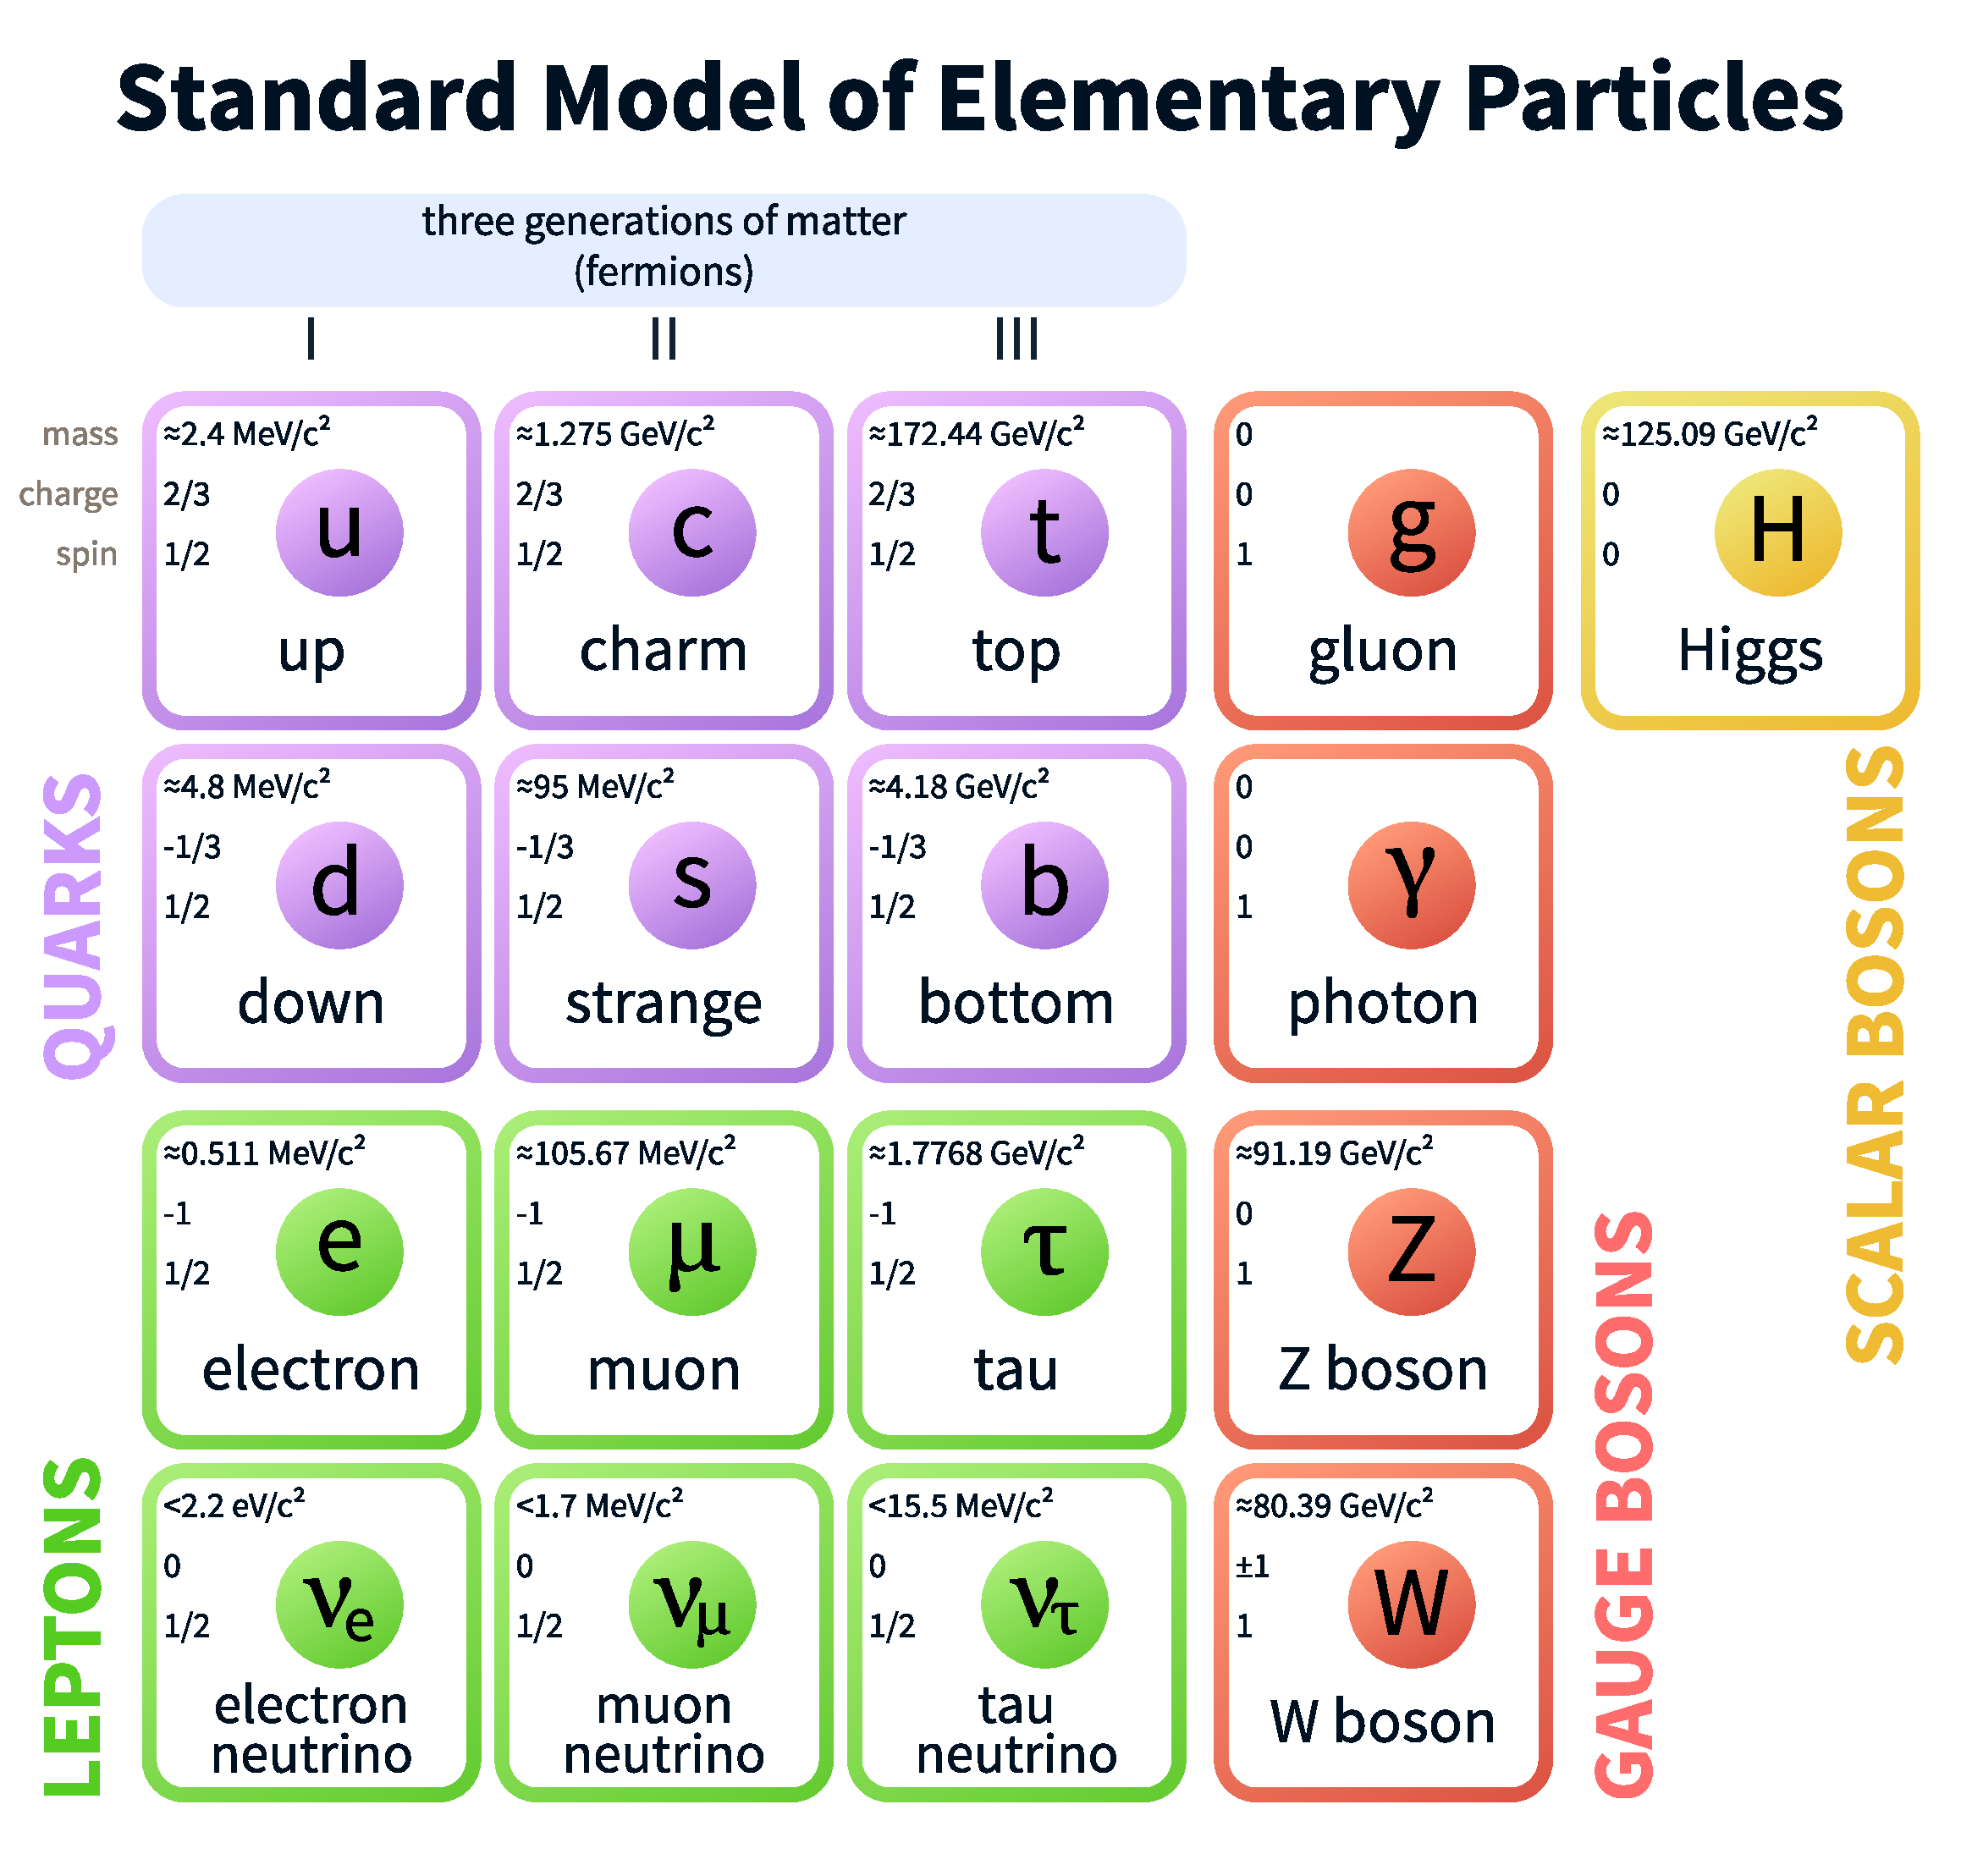
\includegraphics[width=0.75\textwidth]{figures/standard-model-light.pdf}
  \caption%[A diagram of all the particles of the Standard Model,
          %grouped into families of related particles.]
  {A diagram of all the particles of the Standard Model, grouped into
  families of related particles. Mass measurements are constantly
  being improved, and the listed mass values may not reflect the latest and
  best measurements.}
  \label{fig:standardmodel}
\end{figure}

\subsubsection*{Quarks}
There are six quarks in the SM. In order from lightest to heaviest,
these quarks are named \emph{up, down, strange, charm, bottom,} and
\emph{top}. They are often referred to using only the first letter of
their names. Up and down quarks are essential to our lives, as
they make up the nuclei of atoms: the proton is composed of two up
quarks and a down quark bound together ($uud$), and the neutron is composed of one up
quark and two down quarks ($udd$) bound together. The four heavier
quarks tend to decay into lighter quarks within a fraction of a
second, so they are generally not found in everyday matter. The up,
charm, and top quarks all have a positive charge with $\frac{2}{3}$ the
magnitude of the electron's charge, and the down, strange, and bottom
quarks have a negative charge that is $\frac{1}{3}$ that of the electron.

The top quark has several unique properties that make it important
in particle physics. Not only is
it the heaviest quark, but it is also the heaviest elementary particle
we know of, with a measured mass of approximately 173 giga-electron
volts (GeV). This figure is comparable to the mass
of an entire tungsten atom, which contains a multitude of quarks and
electrons. For comparison, the mass of the up quark is approximately
2.2 mega-electron volts (MeV) \cite{pdg}.
In addition, when the top quark decays, it has a 96\% chance of
decaying into a bottom quark and a W boson \cite{pdg}. Few other
particles have such predictable decay products. The reasons why these
properties are so important will be articulated in later chapters. % Specific reference?

\subsubsection*{Leptons}
There are three defining members of the lepton family. In order of
increasing mass, they are: the electron
($e^-$), the muon ($\mu^-$), and the tau ($\tau^-$). As their symbols
denote, these leptons each have a negative electric charge. They are
often referred to collectively as the charged leptons.
The electron is well known as the part of an atom responsible for the
majority of its chemical interactions with other atoms. Muons and taus
tend to decay within a fraction of a second, so they also tend not to
be found in everyday matter. However, muons are often produced in
Earth's upper atmostphere due to bombardment by cosmic rays, particles
streaming in from outer space \cite{griffiths}.

For each charged lepton, there is a corresponding particle called a
neutrino. They are the electron neutrino ($\nu_e$), the muon
neutrino ($\nu_{\mu}$), and the tau neutrino ($\nu_{\tau}$). As their
name suggests, neutrinos are electrically neutral - they have no
charge. In addition, neutrinos have extremely small masses. In fact,
the SM considers them to be massless particles, but experimental
results show they have non-zero masses of less than one electron volt
(eV) \cite{pdg}. Neutrinos also have an extremely small probability of
interacting with matter. In practice, this makes neutrinos
difficult or impossible to detect. The experimental implications of
this fact will be described in chapter \ref{chap:hardware}. % Reference a more specific section once written?

\begin{figure}[h]
  \centering
  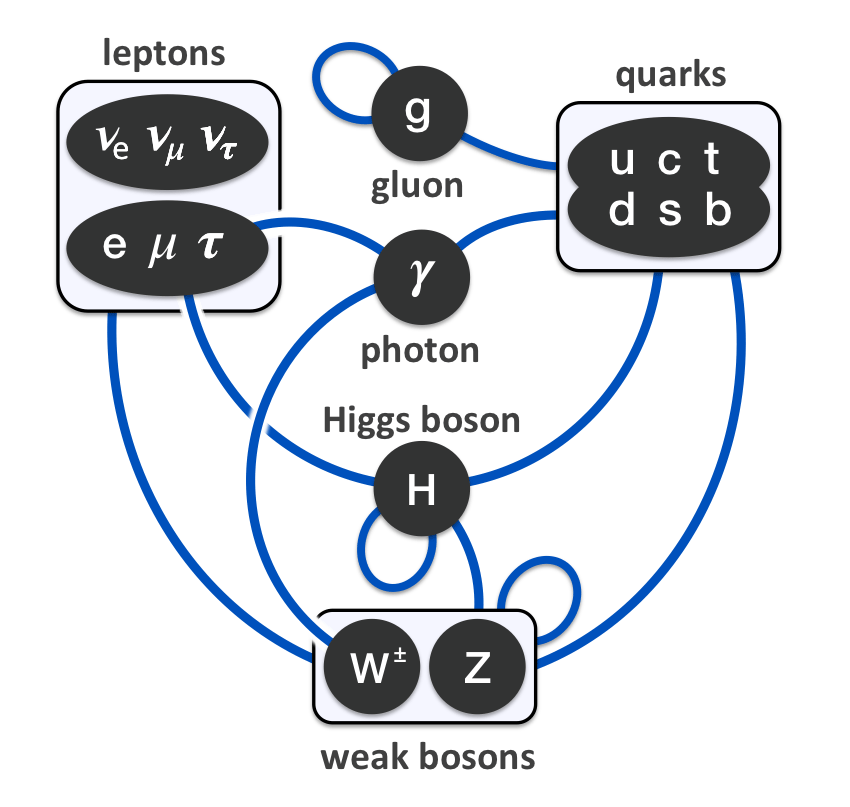
\includegraphics[width=0.75\textwidth]{figures/couplings.png}
  \caption{A diagram of the interactions, or couplings,
    between the particles of the Standard Model. Particles or groups
    of particles connected by blue lines are able to interact with
    each other.}
  \label{fig:couplings}
\end{figure}

\subsubsection*{Force Carriers}
The Standard Model describes four force-carrying particles. These
particles are the physical manifestations, or \emph{quanta}, of the forces
they convey. In general, matter particles interact with other matter
particles through the force-carriers. However, not all particles are
able to interact with all forces.

The photon ($\gamma$), commonly known as the particle of light,
is in fact the quantum of the electromagnetic
force. Thus every time two particles interact electrically or
magnetically, they do so by exchanging photons. Only particles that
have a non-zero electric charge can interact electromagnetically. Thus
we say the photon \emph{couples to} charged particles. All quarks, as
well as the charged leptons, carry electric charge. The photon travels
at the speed of light, and has no mass or electric charge.

The gluon ($g$) is the carrier of the strong nuclear force. The strong
force is responsible for binding together quarks to form protons,
neutrons, and other composite particles (known collectively as
\emph{hadrons}). This same interaction also causes protons and neutrons to
bind together into atomic nuclei. Gluons couple to any particle
that has so-called \emph{color charge}, namely quarks and
other gluons. Although gluons are in principle massless, the energy of
their collective interactions actually makes up more than 99\% of the
mass of protons and neutrons. % Citation needed! %%%%%%%%%%%%%%%%%%%%%%%%%%

The W and Z bosons ($W^+$, $W^-$, $Z$) carry the weak nuclear force. This
force is best known for mediating radioactive $\beta$-decay through
the W-bosons. In addition, the W boson mediates all Standard Model
processes where a quark or lepton changes flavor. % Citation for flavor-changing neutral current?
Particle physicists know the Z-boson best for its
role in the Drell-Yan process, where pairs of quarks convert into
pairs of charged leptons. The W and Z bosons couple to all matter
particles. In addition, they are capable of coupling to each other,
though such interactions are rare. The W bosons have a mass of around
80 GeV, and the Z boson has a mass around 91 GeV \cite{pdg}.

\subsubsection*{Higgs Boson}
The Higgs boson is included here for completeness, and for the benefit
of the curious reader, although it plays at best a minimal
role in the research described in this dissertation. The Higgs
boson is neither a force-carrying particle nor a matter particle, but
something else entirely. It is the manifestation, or quantum, of the
Higgs field, a field that permeates the entire universe, and endows
mass upon most elementary particles. The top quark is so massive
because it couples very strongly to the Higgs field. Similarly, the
photon is massless because it does not couple to the Higgs field at all.
The Higgs boson was discovered in 2012, and measured to have a mass
of about 125 GeV \cite{jointhiggs}. Thus the Higgs must also couple to itself.

\subsubsection*{Spin}
All particles (both elementary and composite) have
a property known as spin. Spin is an intrinsic property, just like
mass or electric charge. But unlike those properties, spin is quantum
mechanical in nature. So a particle's spin is sometimes called its
spin quantum number. All particles can be divided into two categories
based on their spin quantum numbers: particles whose spin is an
integer (0, 1, 2, 3,$\ldots$) are called \emph{bosons}, and particles whose
spin is a half-integer ($\frac{1}{2}, \frac{3}{2}, \frac{5}{2},\ldots$)
are called \emph{fermions}. Figure \ref{fig:standardmodel}
labels which particles are fermions and which are bosons, but even
absent those labels, you could see that quarks and leptons are all
fermions because they have spins of $\frac{1}{2}$, and the force
carriers and the Higgs particle are all bosons.

\subsubsection*{Antimatter}
For every matter particle, there also exists a corresponding
antiparticle. These are collectively referred to as
antimatter. Antiparticles have mostly the exact same properties as
their normal-matter partners, the key exception being that their electrical charge (if
they have one) is opposite in sign. Thus the anti-electron (also
called a positron) has a positive electrical charge instead of
negative. The antimatter versions of the charged leptons are indicated
with a plus in their symbol ($e^+, \mu^+, \tau^+$), and all other
antiparticles have a bar on top of their symbol ($\bar{u},
\bar{b}, \bar{\nu_{\mu}}$, etc.). When a particle meets its own
antiparticle, they usually produce high-energy photons, or sometimes
Z-bosons. Because antimatter
annihilates on contact with normal matter, it is not found
in large quantities in our universe. However, very small quantities can be
produced by energetic particle collisions in nature, and in manmade
particle colliders.

%%%%%%%%%%%%%%%%%%%%%%%%%%%%%%%%%%%%%%%%
% Do I need to explain Feynman diagrams?
%%%%%%%%%%%%%%%%%%%%%%%%%%%%%%%%%%%%%%%%

\subsection{Successes}
\label{ssec:SMsuccesses}

The predictions of the Standard Model have been borne out in a
staggering number of experiments over the last several decades. This
unprecedented success has led the Standard Model to be labeled as one
of the most successful scientific theories ever formulated. % Probably need a reference for this.
-Give some statistics on number of published particle physics papers
-How many of them substantiate the predictions of the SM?
-Give some examples of remarkable successes (e.g. the Higgs discovery)

\subsection{Shortcomings}
\label{ssec:SMshortcomings}

Despite the Standard Model's vast successes, it is not a complete
theory of all particles and interactions in the universe. Physicists
have observed a number of phenomena that are not described within the
framework of the Standard Model. Additionally, the Standard Model does
not contain all the information needed to
build a stable universe. Some of these shortcomings are presented here.

\subsubsection*{Gravity and the Hierarchy Problem}
When describing the fundamental forces of nature in Section
\ref{ssec:SMdescription}, one force was conspicuous by its absence:
gravity. Although gravity is the most apparent force of nature in our
everyday lives, and was the first to be described mathematically,
the Standard Model is still unable to incorporate the workings of
gravity. Einstein's general theory of relativity does a marvelous job
describing gravity on the scale of large objects, such as stars or
galaxies. However, physicists have so far been unable to formulate a
theory of gravity consistent with quantum mechanics, a necessary step
to incorporate gravity into the Standard Model.

One key stumbling block in the quest to quantize gravity (though by no
means the only one) is called the Hierarchy Problem. In plain language, the
problem is that gravity is weaker than the other fundamental forces by
a staggering 20 to 30 orders of magnitude, depending on the distance
scale considered. Any attempt to unite gravity and the other forces
of nature must find a way to bridge this gulf.

\subsubsection*{Fine Tuning}
Another perceived deficit of the Standard Model is the fact that many
of the fundamental constants of nature are not part of the theory. For
example, the Standard Model predicts the existence of the elementary
particles described above, but it does not predict what their masses will be;
the masses must be measured experimentally. Similarly, the Standard
Model offers no clue to the strength of the various forces of nature,
only their existence. In total, the Standard Model has 19 independent
parameters that cannot be derived from other information in the % Citation for the various free parameters
theory. Some theorists object to this large number as being clunky
and inelegant, feeling that a fundamental description of the universe
should have fewer free parameters.

\subsubsection*{Dark Matter}
Humans have been observing the motions of stars
for longer than recorded history. Starting in the late 19\textsuperscript{th}
century, physicists tried to calculate the mass of the Milky Way
galaxy based on the stars they could see through their
telescopes. They soon discovered that the galactic mass estimated from
visible stars was significantly less than the galactic mass
estimated from the rate at which those stars rotate about the % Citation for 19th century galactic observations
galactic center. In the first half of the 20\textsuperscript{th}
century, scientists noticed the same discrepancy for other galaxies
as well. They hypothesized that galaxies also contained some kind of
matter that was not visible through telescopes (hence \emph{dark}),
but that nevertheless exerted a gravitational pull. In fact, we now % Citation for 20th century galactic observations
estimate that only about $\frac{1}{6}$ of the mass of the universe consists
of visible matter such as stars and planets. % Citation for how much of the universe is made up of what

Since everything is made of particles, the particle physics community
was naturally curious to learn what particles make up dark matter.
Careful astronomical observations and detailed calculations
have shown that dark matter does not interact with the strong or
electromagnetic forces. % Citation needed
However, it is believed to participate in the weak interaction. % Why? Also, citation needed!
Further work has shown that no Standard Model particle (or composite
of Standard Model particles) can have these properties and be
consistent with astronomical observations of temperature and % Ick, I hate how this is phrased. Rewrite!
density. Therefore, the existence of dark matter seems to require
physics Beyond the Standard Model (BSM).

\subsubsection*{Dark Energy}
Observations of the cosmic microwave background (CMB) and of the % When? By whom?
doppler shifts of various stars have demonstrated that the universe is
expanding at an accelerating rate. This result surprised many % Citation for expanding universe
scientists, because the inexorable pull of gravity is expected to slow
the expansion of the universe, until it eventually collapses in on itself. Yet something
is driving an outward push that is speeding up instead of slowing
down. Scientists use the term ``dark energy'' to refer to the unknown
and unobserved energy driving this expansion.
% Does this really necessatate an extension of the SM?
% May be easier to delete this part entirely.

\subsubsection*{Neutrino Masses and Oscillations}
The Standard Model predicts that neutrinos should be entirely
massless. And for many years, observations of processes that produced
neutrinos, such as $\beta$-decay, seemed to confirm this
supposition. However, in 19XX, observations of neutrinos produced in % Year!
the sun showed that the rate of electron neutrinos reaching the earth
was only a third of what was expected. Further experiments eventually % Citation for solar neutrino deficit
revealed that neutrinos actually change back and forth between their three % Citation for neutrino oscillations?
flavors as they travel through space. This mutability made it impossible
for neutrinos to be massless, because massless particles must travel
at the speed of light, and therefore cannot experience the passage of
time. But since neutrinos morph between different states, clearly they
must have some experience of time passing. These
oscillations require an extension of the Standard Model to
explain how neutrinos acquire mass, and how they are able to
change identities.

\section{Supersymmetry}
\label{sec:susy}

Physicists have proposed a number of theories to explain the various
shortcomings of the Standard Model. One particular class of theories,
known as supersymmetry (or SUSY for short), is extremely popular for
the elegant ways it can fill some of these gaps. Although there
are numerous variations of supersymmetric theories, they all have one
defining feature in common. For every Standard Model particle, SUSY
postulates the existence of another particle with mostly the same
properties, but with a spin that differs by $\frac{1}{2}$. Thus every Standard Model
fermion would have a corresponding ``superpartner'' that is a boson,
and every Standard Model boson would have a superpartner that is a
fermion \cite{susyprimer}.

\subsection{Sparticles}
\label{ssec:susysparticles}

Supersymmetry uses a unique, sometimes quirky nomenclature to refer to
the new particles it postulates. The partners of Standard Model
fermions are named by prefixing the existing name with an `s'. Thus
the two families become \emph{squarks} and \emph{sleptons}, and the
individual members of those families are named, e.g., \emph{sup,
  sbottom, selectron, sneutrino}, etc. Meanwhile the partners of
Standard Model bosons gain the suffix \emph{-ino}, which replaces the
suffix \emph{-on} if present. Thus we arrive at the names
\emph{gluino, photino, Zino, Wino}, and \emph{Higgsino}. The symbols
for these particles are generally formed by adding a tilde on top of
the original particle's symbol, so that a scharm squark is notated
$\tilde{c}$, a gluino is notated $\tilde{g}$, etc. To avoid conflict
with the tilde, anti-sparticles are notated using a prime (as in
$\tilde{c}^\prime$) instead of a bar.

These superpartners are capable of mixing with each other to form
different sparticles, which may not correspond exactly to Standard
Model particles. Of particular note are the neutralinos
($\lsp_1, \lsp_2, \lsp_3, \lsp_4$), made by mixing the photino, zino,
and Higgsino; and the charginos ($\chargino_1, \chargino_2$), made by
mixing charged Winos and charged Higgsinos.

It is worth noting that if SUSY were a perfect symmetry, all
sparticles would have the same masses as their corresponding
particles. However, to date, no sparticles have been
observed, implying that most sparticles (if they exist) must be too
heavy to produce using our current particle colliders. Since the
equality of masses is destroyed, we say SUSY is a \emph{broken
  symmetry} \cite{susyprimer}.

\subsection{Rationale}
\label{ssec:susyrationale}

One of the features that makes SUSY very attractive is its ability to
solve the hierarchy problem. The exact nature of this solution
invokes complicated mathematics, and is not terribly pertinent to the
research described in this dissertation. However, it revolves around
the notion that the introduction of several new massive sparticles
creates substantial corrections to the square of the mass of the
Higgs boson ($m_H^2$) \cite{susyprimer}.
% However, the essence is
% that the massive Standard Model particles should make the Higgs mass
% squared ($m_H^2$) blow up to an enormous value; by introducing a
% new boson for every SM fermion, and vice-versa, SUSY cancels out
% the effects of the SM particles, and allows $m_H^2$ to take on a
% more reasonable value \cite{susyprimer}.

In addition, SUSY provides particles that may be good candidates to
explain dark matter. At the moment, the most popular explanation for
the composition of dark matter is weakly-interacting massive particles
(WIMPs). These are particles that primarily interact through the weak
force, and that also have mass, allowing them to exert a gravitational
pull. The neutralinos fit this bill nicely. In addition, the dark
matter particle must be stable. The lightest supersymmetric particle
(LSP) is expected to be stable due to conservation laws associated
with supersymmetry, and many SUSY models predict that the lightest
neutralino, $\lsp_1$, actually \emph{is} the LSP. Thus the lightest
neutralino makes a tantalizing dark matter candidate
\cite{susyprimer}. We will assume moving forward that $\lsp_1$ is the
LSP, and will use the two terms interchangeably.
% Need citation for this stuff?



% Chapter that introduces the LHC and the CMS experiment
\chapter{The Large Hadron Collider and the CMS Experiment}
\label{chap:hardware}

In order to study the properties of the Standard Model particles, and
to search for physics beyond the Standard Model, we need a way to
produce particles other than the simple up and down quarks and
electrons that make up everyday matter. And once we have produced
particles, we need a way to detect their presence, identify them, and
measure their properties.

This chapter will describe the hardware used to perform
the analyses described in Chapters \ref{chap:afb} and \ref{chap:stop},
namely the Large Hadron Collider and the CMS Detector. In addition, it
will describe how the CMS Collaboration uses software to make sense of
the readings it has collected from the CMS detector. Because these
systems are immensely complex, this chapter will not attempt to be
totally comprehensive, but will focus on the elements that are most
important for understanding the science presented in the next two
chapters. % Review to see if I'm actually meeting this goal

\section{The Large Hadron Collider}
\label{sec:lhc}

In order to study heavy particles, we must first create them, since
they are hard (or even impossible) to find in nature.
Einstein's famous equation, $E = mc^2$, tells us that mass and energy
are equivalent to one another. Physicists employ this principle to create
heavier particles by taking lightweight particles, accelerating them to very high
speeds, and smashing them together. Particles moving at high speed
have high kinetic energy, and when those particle collide, that energy
can be converted into mass, creating heavier particles. Because it is
so often conducted at high energies, particle physics is sometimes
referred to as high energy physics, or HEP.

The Large Hadron Collider, or LHC, is currently the largest and most
powerful particle collider ever built. % cite the LHC published description
It is currently the flagship experiment of CERN, the European Organization
for Nuclear Research, located in Geneva, Switzerland.
The LHC is a ring-shaped structure some 27 kilometers in circumference,
buried underground beneath the border between Switzerland and
France. The ring encloses two pipes, through which beams of
protons normally circulate in opposite directions. Strong electric fields
propel the protons along the beam pipes, and strong magnetic fields
steer the protons around the ring.

% Pictures of the LHC from above, and the tunnel.
% And maybe a cross-section of the machine.

The LHC is fed by a chain of smaller accelerators at CERN that shape
the beams and bring them partway up to speed so they can be injected
into the LHC. The LHC was designed to collide protons at an energy of
14 trillion electron-volts (TeV). However, during early testing, a
defective weld caused severe damage to the LHC; as a precaution
against future damage, the LHC was operated at 7 and 8 TeV energy in
its first run (Run I), and has been colliding at 13 TeV so far in its
second run (Run II). At these energies, the protons in the beam are
moving at 99.99999999\% of the speed of light.

The proton beams are not continuous streams of particles. Rather, the
protons are grouped into bunches. During Run I, the LHC circulated XX
bunches of YY particles. These bunches were spaced so that collisions
could be made to occur every 50ns, or 20 million collisions per
second. Currently, in Run II, the LHC circulates XX bunches of YY protons, and
collides them every 25ns (40 million collisions per second). % Bunch size and spacing needed!
Each beam crossing is referred to as an ``event''. A single event may
contain multiple collisions between protons in the bunches. % Explain what pileup is

% Explain luminosity (give the n = l * sigma equation)
% Also good to explain integrated luminosity

Although we have been describing protons as simple particles, in fact
they are anything but. Protons contain two up quarks and a down quark,
and innumerable gluons binding them together. But in addition, protons
contain a sort of froth of quarks and antiquarks that are constantly
popping into and out of existence on ultrashort timescales, in
accordance with the laws of quantum mechanics. Collectively, all of
these components of a proton are known as \emph{partons}, and any of
them may be involved when two protons collide. Studies on the relative
momentum of these various partons tell us that at the LHC, most of the
time it is the gluons that are colliding with each other. % Citation?

At four places around the LHC ring, the beam pipes intersect, and the
proton beams are made to collide with one another. At each of these
four locations, a detector is placed where it can observe the
particles that are produced by these collisions. Two of
the detectors are large, general-purpose machines, designed to support
a wide variety of particle physics research. These detectors are called CMS
and ATLAS. There are two general-purpose detectors so that the results from one
may be cross-checked by the other. The other two main
detectors are moderately sized and designed to study specific kinds of physics
phenomena. One is LHCb, which is designed to study the physics of
bottom quarks. The other is ALICE; a few weeks each year, the LHC
collides lead nuclei instead of protons, and ALICE is designed to
study the physics of these collisions. In recent years, three smaller detectors have
been added: ToTeM, which shares an interaction point with CMS; MoEDAL,
which is colocated with LHCb; and LHCf, installed around the ATLAS detector.

\section{The CMS Detector}
\label{sec:cms}

% Should be citing the original CMS detector description paper!!

The research described in Chapters \ref{chap:afb} and \ref{chap:stop}
was conducted using data gathered on proton-proton collisions by the
CMS detector. CMS stands for Compact Muon Solenoid, a name whose
origin will become apparent in the next few sections. In brief, though,
this detector is a complex, multilayered array of sensors designed to
detect and measure the properties of as many of the particles emerging
from the collision point as possible.

% Wedge diagram goes here

The CMS detector is composed of multiple layers, each with a specific
purpose. These layers work in concert to provide a fairly complete
picture of the numerous particles emerging from a collision.
Figure \ref{} shows a small cross-sectional wedge
of the detector, and demonstrates how each of the components
contributes to measurements of the particles produced in the
collisions.

The CMS detector was designed with a wide array of physics goals in
mind. Some of these goals included discovering the Higgs boson,
especially in decays to leptons or photons; discovering signs of
supersymmetry, if such signs existed; searching for extra
dimensions; and conducting precision tests of the predictions of the Standard Model.
These and other goals had to be balanced against practical
constraints, such as budget, durability, and ease of readout. The
detector that resulted from the convergence of these factors is
described in Sections
\ref{ssec:cms:components:magnet}-\ref{ssec:cms:components:muon}.

\subsection{Coordinates}
\label{ssec:cms:coordinates}

% Insert pictures that show detector coordinates

Before we can understand the design of the CMS detector, or the
physics it studies, we must assign a coordinate system to the detector.
Because the beam pipe has cylindrical symmetry, the CMS detector is
similarly cylindrical. It is shaped like a giant barrel wrapped around
the beam pipe, some 5 stories tall and wide, and 7 stories
long. Figure \ref{} depicts the coordinate system attached to the
detector. The z-axis runs down the center of the beam pipe, and
defines a longitudinal axis. It has a positive and negative direction;
the point $z$ = 0 is the nominal spot where the protons collide. The
azimuthal direction in the detector is measured using the coordinate
$\phi$. The radial coordinate $r$ expresses perpendicular distance from the z-axis.

Because the proton beams are compressed and stabilized in the
transverse plane before they enter the collision area, we expect
that the system of two colliding protons has no net momentum
transverse to the beam pipe. We can therefore expect the total
\emph{transverse momentum} (or $p_T$) of the collision products to be
zero. However, because the individual partons inside a proton have
constantly-changing momenta, we cannot know the total longitudinal
momentum ($p_z$) of the pp collision. For
this reason, we consider the $p_T$ of particles almost exclusively,
and seldom spare a thought for $p_z$.

Because particle collisions take place almost exclusively near the
origin of the detector and their components spread out from there, it
is sometimes helpful to describe the trajectories of particles in terms of
a sort of angle that they make in the $r-z$ plane. We could use the
polar angle $\theta$ from spherical coordinates. But in a world of
particles moving at relativistic speeds, we will often need to boost
between different reference frames, and $\theta$ becomes
cumbersome. Physicists came up with a more useful coordinate, which
they termed \emph{rapidity}. In collider physics, the rapidity, $y$,
of a particle is given by:
\begin{equation}
\label{eq:cms:rapidity}
y = \frac{1}{2} \ln \frac{E+p_z}{E-p_z}
\end{equation}
This coordinate has the advantage of transforming simply under Lorentz
boosts. If two reference frames differ by a relativistic velocity
$\beta = v/c$, then the rapidity in the new frame is given by $y\prime
= y - \tanh^-1 \beta$. And because of this easy transformation rule,
the rapidity difference $\Delta y$ between two particles is Lorentz
invariant--it remains the same no matter what reference frame it is
measured in.

Rapidity will be used to define other variables in Section
\ref{ssec:afb:variables}, but on the whole, it turns out to be not
very convenient, because it requires us to know the energy of the
particle. So physicists have devised a related quantity that behaves
somewhat better, calling it \emph{pseudorapidity}. The pseudorapidity,
$\eta$, of a moving particle is defined by
\begin{equation}
\label{eq:cms:eta}
\eta = -\ln \left[ \tan \left( \frac{\theta}{2} \right) \right]
\end{equation}
This coordinate depends only on the polar angle, not the energy, of a
particle. And like its cousin, the pseudorapidity difference $\Delta\eta$
between two particles is also a relativistic invariant. In fact, at
velocities approaching the speed of light, rapidity and pseudorapidity
become equal to one another. $\eta$ is used widely in collider
physics, even to the extent that parts of the CMS detector are
referred to by their ($\eta, \phi$) coordinates.

% Explain Delta R as a measure of distance (or cone size)

% Describe the barrel and endcap regions. Necessary for explaining the
% geometry of the components.


\subsection{Superconducting Solenoid}
\label{ssec:cms:components:magnet}

The defining feature of CMS, which gives rise to the 'S' in its name,
is the superconducting solenoid. This component is a large
electromagnet; it is made from superconducting niobium-titanium
material, taking the form of a giant coil 12.9m long and with an inner
bore of 5.9m \cite{tdr}. When cooled to about 4 Kelvin using liquid helium,
the magnet can generate a longitudinal magnetic
field of up to 4T inside the solenoid, though in practice we run it at
3.8T to help it last longer. The return field outside the
solenoid is lower, and is not uniform \cite{accelexper}.

The purpose of this magnet is to bend the trajectories of particles
passing through the detector. The tracker and the muon system
(described below) can measure the radius of curvature of a track, from
which we can determine how much momentum the particle was
carrying. The strength of the magnetic field was chosen based on
the requirement that the CMS detector be able to determine the charge
of a muon carrying 1 TeV of momentum \cite{tdr}.

\subsection{Inner Tracker}
\label{ssec:cms:components:tracker}

The innermost component of the detector, wrapped immediately around
the beam pipe, is the inner tracker. This component is made of several
layers of silicon sensors. Every time a charged
particle passes through a layer of silicon, it creates a blip of
electrical current in the silicon that can be read out
electronically. We can ``connect the dots'' to reconstruct the path
the particle took. Because of the magnetic field inside the detector,
charged particles will have curving trajectories. Using the tracker,
we can measure the radius of curvature of these tracks, and thus
determine the momentum of the particle that created the
tracks. Because the magnetic field is only in the z-direction, we can
only measure the $p_T$ of the charged tracks, not the
$p_z$. Importantly, neutral particles do not leave any hits in the
tracker, and thus their trajectories cannot be measured.

% Figure of the tracker geometry

Figure \ref{} shows the geometry of the tracker as originally designed.
The innermost part of the tracker ($r \lesssim$ 10cm), where the tracks are densest,
consists of silicon pixels. At installation, there were three pixel
layers in the barrel and two in the endcaps. Each pixel is
100$\times$150 $\mu$m in size. At this scale, the expect occupancy of
a pixel was $10^{-4}$ per bunch crossing \cite{tdr}. The pixel tracker
was upgraded during the 2016/2017 winter shutdown, adding a fourth
pixel layer in the barrel and a third in the endcaps, while slimming
down the hardware that supports the functioning of the pixels
\cite{pixeltdr}.

The remaining layers of the tracker consist of silicon strips. In the
region $20 < r < 55$ cm in the barrel (Tracker Inner Barrel, TIB),
there are four layers of silicon
microstrips, with a size of at least 10 cm $\times$ 80$\mu$m. In the
Tracker Outer Barrel (TOB), defined by $r >$ 55cm, there are six
layers of microstrips with a size of no more than 25 cm $\times$
180$\mu$m. In the endcap regions, the Tracker Inner Disks (TID) sit
just outside the TIB, and consist of threel layers of disks of
strips. The Tracker Endcaps (TEC) sit just outside the TOB, and
consists of nine disks of silicon strips. These various layers provide
tracker coverage out to $|\eta| \approx 2.5$.

The electrical impulses produced in the silicon pixels and strips are
read out by ``APV25'' chips that amplify and process the signals. The
signals are then passed out of the detector using optical cable, and
further processed in hardware outside the detector itself
\cite{tdr}. Additional hardware circulates a refrigerant liquid that
maintains the silicon sensors at a temperature no higher than
$-10^\circ$ C \cite{accelexper}. The materials and geometry of the
original tracker are chosen to minimize the amount of energy absorbed
from particles as they pass through. The original
tracker had a radiation thickness of about $0.4 X_0$ at $\eta = 0$,
increasing to a maximum of $1.0 X_0$ at $|\eta| = 1.6$ and dropping
back to $0.6 X_0$ at $|\eta|=2.5$, \cite{tdr}. The radiation length,
denoted $X_0$, will be explained in the ECAL discussion next.
% Consider pulling plot of material budget

The performance of the inner tracker has been measured using both
muons and pions. For muons with $p_T$ of 100 GeV, the resolution
in $p_T$ is about 1.5-2\% up to $|\eta|$ of 1.6, beyond which the
resolution worsens exponentially. For muons with $p_T$ of 10 or 1 GeV,
the resolution is better, on the order of 0.5-1.0\%. The efficiency of
global muon track reconstruction is generally around 99\% for $p_T$ of
1, 10, or 100 GeV, with a slight dropoff at $\eta=0$ and an
exponential faloff above $|\eta|$ of 2.0. For pions, the global track
resolution is somewhat less, ranging from 85-95\% for 100 GeV pions and
75-90\% for 1 GeV pions \cite{tdr}.
% Consider pulling some of the resolution plots

\subsection{Electromagnetic Calorimeter (ECAL)}
\label{ssec:cms:components:ecal}

Just outside the tracker, the next component in the CMS
detector is the electromagnetic calorimeter, or ECAL. The purpose of
this device is to measure the energy of electromagnetic particles
(electrons and photons) emitted from the collisions. The ECAL consists
of a giant array of lead tungstate (PbWO$_4$) crystals; when struck by
electromagnetic particles, these crystals scintillate with a
pale blue light that can be read out by optical sensors. The amount of
light gives us a measure of how much energy the particle was
carrying. In addition, the pattern of energy deposition in the
crystals can provide information useful in particle
reconstruction.

Lead tungstate has a number of properties that make it an ideal
material to use in the ECAL. For one thing, it is quick to read
out: lead tungstate crystals can release 80\% of their scintillation
photons in the 25ns window between proton bunch crossings. In
addition, lead tungstate is highly resistant (``hard'') to the high
levels of radiation emitted by the collisions, tolerating a total
absorbed dose of up to 10 Mrad (100 kGy). But perhaps most importantly,
lead tungstate allows the ECAL to be built relatively compactly,
because the material has a short radiation length ($X_0$) and
Moli\`{e}re radius ($R_M$).

Radiation length and Moli\`{e}re radius are two properties that
describe a material's ability to absorb electromagnetic energy. When
an electron passes into a material, the radiation length is the
characteristic distance over which that electron will lose all
but 1/$e$ of its energy. To put it mathematically:
\begin{equation}
\label{eq:cms:ecal:radlength}
E(x) = E_0 \cdot e^{-x/X_0}
\end{equation}
It is also equal to 7/9 of the mean free path for pair production by
photons \cite{pdg}. So the shorter the radiation length for a
material, the shorter the distance needed for electromagnetic
particles to be stopped and their energy absorbed. Lead tungstate has
a radiation length $X_0 = 0.89$ cm \cite{tdr}. Similarly, the
Moli\`{e}re radius governs the absorption of energy in the direction
transverse to the particle's trajectory. It is the characteristic
lateral distance over which 90\% of an EM shower's energy will be
contained. So materials with a shorter Moli\`{e}re radius will have on
average a smaller transverse shower size. For lead tungstate, $R_M =
2.2$ cm \cite{tdr}. These characteristic distances will play a role in
determining the size of the ECAL crystals.

The ECAL is divided into two regions: the barrel, and the
endcaps. These may be seen in Figure \ref{}.
The PbWO$_4$ crystals are shaped like tapered rectangular prisms. In
the barrel region, they are 230 mm long, corresponding to 25.8 $X_0$,
and have front faces that are 22$\times$22 mm, corresponding to
1$\times$1 $R_M$. These dimensions ensure that very little EM energy
will escape out the back of the crystals, and that
about 94\% of a given shower will be contained in a 3$\times$3 array
of crystals. In the endcaps, the crystals are 220 mm long (24.7 $X_0$),
and have front faces of 28.6$\times$28.6 mm (1.3$\times$1.3 $R_M$).
The barrel section is composed of 36 ``supermodules''. Each
supermodule is an array of 85$\times$20 crystals, covering half the
barrel length and 20$^\circ$ in $\phi$. Each of the two endcaps is
composed of two half-circle structures called ``Dees''. Each dee holds
138 groupings of 5$\times$5 crystals (called``supercrystals'') plus
18 partial supercrystals. The endcaps are also fronted with preshower
detectors, whose purpose is primarily to study neutral pions produced
at high $\eta$. These preshower detecters are composed of lead
absorbers that initiate pion showering, and silicon strip detectors
that measure the size and shape of the shower. All told, there are
75,848 crystals in the entire ECAL, providing very fine spatial
granularity. As Figure \ref{}
shows, ECAL coverage extends out to $|\eta|$ = 3.0. However, there is
a gap in coverage between the barrel and the endcaps. Electromagnetic
particles that fall into this ``crack'' will not be measured, a fact
that we must account for when attempting to reconstruct electrons and
photons \cite{tdr}.

% Pull TDR figure 4.1

Lead tungstate produces a blue-green scintillation light, peaking near
420mm. The amount of light produced in each crystal must be measured,
and the information digitized, in order to determine the energy of incident EM
particles. This presents a slight problem. Despite its other admirable
properties, lead tungstate produces relatively little scintillation
light - about 30 photons per MeV of energy. This fact necessitates
the use of systems that can amplify faint signals. In the
barrel, photons are read out by silicon avalanche photodiodes (APDs)
stuck to the backs of each crystal. In the endcaps, vacuum
phototriodes (VPTs) are used for readout instead. These sensors feed
their signals to amplification and digitization hardware attached to
the CMS detector, and from there are sent to computing equipment
outside the detector volume \cite{tdr}.

The performance of the ECAL was measured using a controlled beam of
electrons. The measured energy resolution in groups of 3$\times$3
crystals is shown in Figure \ref{}.
This resolution function was parameterized by a Gaussian fit of the form
\begin{equation}
\left( \frac{\sigma}{E} \right)^2 =
\left( \frac{S}{\sqrt{E}} \right)^2 +
\left( \frac{N}{E} \right)^2 + C^2
\end{equation}
where $S$, $N$, and $C$ are parameters representing the stochastic,
noise, and constant contributions to the resolution, respectively. As
Figure \ref{} shows, the energy resolution is better
than 1\% for electron energies above about 20 GeV \cite{tdr}.

% Stick in TDR figure 1.7

\subsection{Hadron Calorimeter (HCAL)}
\label{ssec:cms:components:hcal}

Outside the ECAL but (mostly) inside the magnet lies the hadron
calorimeter, or HCAL. This component is designed to measure the energy
of hadronic particles produced in collisions. The HCAL is composed of
alternating layers of metal, used to absorb some of the incident
hadronic energy, and scintillating materials, used to measure the
hadronic energy deposited in the calorimeter. The HCAL thus has an
important role in measuring the energy of jets, as well as in
measuring pileup from secondary collisions in the event.

The power of materials to stop relativistic particles is described in
terms of the interaction length, $\lambda_I$. When a number of
particles are incident on some material, this parameter describes
the length over which all but a 1/$e$ fraction of those particles will
be absorbed. In other words:
\begin{equation}
\label{eq:cms:hcal:intlength}
N(x) = N_0 \cdot e^{-x/\lambda_I}
\end{equation}
So the shorter a material's interaction length, the shorter the
distance over which it will absorb incident particles.

The CMS HCAL is a \emph{sampling} calorimeter, meaning that it uses
different materials to produce the shower and to measure the
energy. Hadronic showering is induced by the absorber layers, most of
which are made of brass (70/30\% Cu/Zn). Brass
is used because it is relatively affordable, and also because it is
non-magnetic, and thus won't perturb the magnetic field inside the
detector. This particular brass alloy has an interaction length
$\lambda_I = 16.42$ cm. Stainless steel is also used as an absorber in places.
Interleaved with the absorber materials are layers of
scintillating material. Most of the scintillators are made of
radiation-hard plastic, either Kuraray SCSN81 or Bicron BC408, though
where extreme particle flux and radiation is an issue, quartz fiber is
used instead for its superior radiation hardness.

The HCAL is divided into four subcomponents: the barrel (HB), the
endcaps (HE), the outer calorimeter (HO), and the forward calorimeter
(HF). Each of these components operates on the same principles, though
the design of each differs slightly. These components are all cleverly
overlapped to avoid any cracks like that of the ECAL.

The barrel covers the range $|\eta| <$ 1.3. The absorber material in
the HB is segmented into 36 wedges; each wedge encompasses half the
length of the HB and 20$^\circ$ in $\phi$. There are 16 layers of
absorber material in each wedge; the innermost and outermost layers are
made of stainless steel, for strength, and the middle 14 layers are
brass. The total thickness of these absorber layers is 5.82
$\lambda_I$ at $\eta$ = 0, increasing to 10.6 $\lambda_I$ at $|\eta|$
= 1.3. Within each wedge, the scintillating material is further
divided into segments of size 0.087$\times$0.087 in $(\Delta\eta,\Delta\phi)$
space, providing fine granularity. The innermost layer of
scintillating material in the HB is Bicron BC408, and the remaining 16
layers are Kuraray SCSN81 \cite{accelexper}.

The endcaps cover the regions 1.3 $< |\eta| <$ 3.0, and use the same
absorber and scintillator materials as the barrel, with one exception:
stainless steel is only used as the outer absorber layer, to
prevent any magnetic interference inside the magnet bore. The
scintillators are divided into segments of size 0.087$\times$0.087 in
$(\Delta\eta,\Delta\phi)$ space for $|\eta| <$ 1.6, and approximately
0.17$\times$0.17 for $|\eta| \geq$ 1.6. The total thickness of the
endcaps (including attached ECAL dees) is about 10 $\lambda_I$
\cite{accelexper}.

The outer calorimeter is designed to augment the stopping power of the
HB and the EB, and covers the region $|\eta| <$ 1.3. It consists of
tiles of Bicron BC408 scintillator embedded in the iron yoke that
gathers the returning magnetic field outside the solenoid. Thus the HO
actually uses the solenoid material itself as an absorber.
Following the shape of the return yoke, the HO is divided into 5 rings
along the $z$-axis, each of which has 12 sectors in $\phi$. There are
gaps between the rings and in some azimuth sectors for the cryogenic
and power lines that supply the magnet. The scintillator tiles roughly
follow the 0.087$\times$0.087 segmentation of the HB, within the
constraints of the yoke geometry \cite{accelexper}.

The forward calorimeter is located in the region 3.0 $< |\eta| <$
5.2. This area receives an extremely high flux of particles due to its
small angle with respect to the beamline. As such, this component
must be considerably more radiation hard than any other part of the
HCAL. To meet this requirement, the HF uses quartz fibers with polymer
cladding as its measuring material, and reads out Cherenkov light rather than
scintillation light. Each end of the HF is composed of stainless steel
absorbers arranged in 18 azimuthal wedges, each of which is penetrated
by quartz fibers that run parallel to the beamline. Some of these
fibers only penetrate partway through the steel plate, allowing the HF to
differentiate between electromagnetic and hadronic showers based on
penetration depth. The fibers form towers of size 0.175$\times$0.175
in $(\Delta\eta,\Delta\phi)$ space \cite{accelexper}.

The scintillation light from the plastic tiles is read out by
Kuraray Y-11 wavelength-shifting (WLS) fibers. These fibers are embedded
into the tiles themselves. Once outside the tiles, the WLS fibers are
spliced to clear optical fibers that send the light to hybrid
photodiodes for electronic processing. The Cherenkov light from the
quartz fibers is transmitted to air-core light guides, which carry the
light through layers of radiation shielding to photomultiplier tubes
outside the shielding \cite{accelexper}.

% Resolution/performance?
   % Figure 1.8 apparently shows that JER as a function of ET is similar in all parts of the HCAL
   % MET resolution function is given in 1.5.4.5
   % May need to see TDR chapter 11? (This according to 1.5.4.5).
   % See also TDR 5.4?

\subsection{Muon System}
\label{ssec:cms:components:muon}

The outermost component of the CMS detector is the muon system. The
strong penetrating power of muons allows us to place this system
outside all the other layers without fear that the muons will be
absorbed en route. As its name suggests, the muon system is
responsible for measuring the momentum of muons as they fly away from
the collision point. It employs three different gas-and-electrode
technologies to reconstruct the trajectories of muons, from which
momentum can be inferred. These trajectories can be combined with
measurements from the tracker for greater precision.

% Insert Fig. 1.6 from the TDR

The layout of the muon system is presented in Figure \ref{}.
Like many other components, it is divided into barrel and endcap
regions. The barrel region detects muons using a combination of drift
tubes (DTs) and resistive plate chambers (RPCs), whereas the endcaps use cathode
strip chambers (CSCs) and RPCs. All three of these technologies detect
muons by the trail of ionization they leave after passing through a gas. The
liberated electrons will be attracted to positively charged
electrodes, and the ions to negatively charged electrodes. When
electrons and ions hit the electrodes, they produce an electrical
signal that is read out, and timing information
is used to tell how far along the electrode the impact occurred.
The drift tubes are long, thin chambers filled with a mixture of 85\%
Ar and 15\% CO$_2$ gases, and with a positively charged wire running
down their centers. Drift times in these chambers are a maximum of 380
ns. These tubes provide 1D position measurements, but multiple layers
may be stacked at right angles to
provide 2D measurements. These devices are used because they are precise
and inexpensive, and can function well in the muon barrel, where the
particle flux and magnetic field are both low
\cite{accelexper,websitedt}. The cathode strip chambers are planar
chambers filled with a mix of 40\% AR, 50\% CO$_2$, and 10\%
CF$_4$. They contain positively charged wires running in
one direction, and negatively charged strips running perpendicularly,
providing native 2D position measurements. CSCs are employed in the
endcap because they are precise, moderately fast ($<$ 225 ns), and can operate
in the high magnetic fields at the fringes of the solenoid
\cite{accelexper,websitecsc}. Resistive plate chambers are planar
chambers filled with a mixture of 96.2\% C$_2$H$_2$F$_4$, 3.5\%
$i$C$_4$H$_{10}$, and 0.3\% SF$_6$. They have a positively charged
plate on one face, and a negatively charged plate on the
opposite face. Electrons are actually detected by metal strips just outside
the chambers. RPCs are used to supplement the DTs and CSCs
mainly for their 1 ns timing resolution; their spatial
resolution is not as fine as the DTs or the CSCs
\cite{accelexper,websiterpc}. The signals from these subsystems are
processed in electronics both within the detector volume and outside it.

The barrel section of the muon system, covering $|\eta| <$ 1.2, is
interleaved with the iron return yokes, structures that concentrate
the magnetic field exiting the solenoid and return it around to the
other end. As such, the muon barrel follows the geometry of the
yokes. The return yokes consist of five rings % width of the rings?
and divided into 12 sectors in $\phi$. As Figure \ref{} shows,
the DTs and RPCs are stacked in four layers, or \emph{stations}. These
are offset in $\phi$ so that all muons will pass through at least
three. The three innermost stations contain 12 planes of DTs, 8 of
which provide $r-\phi$ measurements, and 4 of which provide $z$
measurements. The outer station lacks the $z$ measuring planes. The
inner two stations are coupled to two RPCs each, and the outer two
stations have one RPC each. With this geometry, each individual
station can provide position measurements with a precision of better
than 100 $\mu$m in space and about 1 mrad in $\phi$ \cite{tdr}.

The endcap muon system covers the range 0.9 $< |\eta| <$ 2.4. The
CSCs are arrayed in four layers of disks, with each disk being made up
of several trapezoidal chambers 10 or 20$^\circ$ wide in $\phi$,
arranged in concentric rings. Each chamber contains 6 gas gaps and
electrode grids. There are 36 chambers in each ring, except the
centermost rings of stations 2-4, which have only 18 chambers. The
CSCs provide a spatial resolution of about 200 $\mu$m and an angular
resolution in $\phi$ of about 10 mrad \cite{tdr}. During Run I, the
first three disks had RPCs attached to all but the central ring; for
Run II, the outer CSC ring of disk 4 was added, and was instrumented
with attached RPCs.

% Anything I want to say about cosmics?

\section{Triggers}
\label{sec:cms:triggers}

As previous sections have described, the LHC collides protons at a
rate of 40 million collisions per second. However, the number of
collisions per second that can actually be recorded is ultimately
dictated by the medium used to store the data. Magnetic disk drives
are prohibitively slow for our uses, while solid-state
drives are prohibitively expensive. So in particle physics, we store our data
on magnetic tape (like one might find in a video or audio
cassette). The data recording system allows us to keep only about one
of every 100,000 events.

Fortunately, this constraint is less harmful than it might seem,
because not every event is worth saving. Even with the
considerable beam focusing power of the LHC, most bunch crossings only produce
near-misses or grazing contact between protons. True head-on pp
collisions, producing particles with a high transverse component to
their momentum, are somewhat rare. Thus we can reach our threshold of
1000 events per second by using a system of ``triggers'' to store only
events where interesting physics is taking place.

The first stage of the trigger system is the Level 1 trigger
(L1). The L1 trigger is integrated directly into the detector
hardware, and does not use any computational resources. It
is tripped by basic signatures such as ionization tracks in the muon system, ECAL
deposits consistent with electrons or photons, HCAL deposits
consistent with jets, and a few others. This trigger system is able to
make extremely fast decisions, and outputs events at a rate of 100
kHz \cite{trigger}.

Events passing the L1 triggers are handed off to the second trigger
stage, called the high-level trigger (or HLT). This stage uses
banks of commodity computers running physics reconstruction
software to make a much more sophisticated determination of what
physics objects are present in the event. Thanks to this more
detailed reconstruction, the HLT allows one to trigger on a wide
variety of signatures, and with a high degree of specificity about
what is desired in the events. The HLT outputs events at an average
rate of about 400 Hz; these are then stored for eventual use in
physics research \cite{trigger}.

The use of these trigger systems can create certain difficulties
that must be compensated for during physics analysis. One
example is that the triggers are not perfectly \emph{efficient},
meaning they miss some fraction of the events they are intended to
trigger on. For instance, a trigger designed to select events
containing muons with $p_T >$ 17 GeV might only select 98\% of those
target muons, and this fraction might even vary with the muon
$p_T$. This effect must be measured, and accounted for when we compare
our data against theoretical predictions. Another problem is that
certain very common signatures (e.g. a single electron) occur more
frequently than the triggers can handle. To cope with this flood of
events, we may have to program the trigger to record only every
$n^\text{th}$ event, and weight that event to count for $n$
events. This is called \emph{prescaling} the trigger. Because
weighting up prescaled events reduces our statistical precision, we
try to use un-prescaled triggers whenever possible.

\section{Reconstruction and Identification}
\label{sec:cms:recoandid}

In order to do meaningful particle physics, we must translate the
output from the CMS detector into a picture of what particles and
objects are present in the event. This is the process of event
reconstruction (``reco'') and particle identification (``ID''). There
are any number of possible algorithms for converting detector
signatures into particles. The CMS Collaboration performs its basic
reconstruction using a system called particle flow (PF).

\subsection{Particle Flow}
\label{ssec:cms:reco:pf}

The particle flow algorithm attempts to associate all of the detector
readings with particles or physics objects. It begins by
reconstructing all the tracks, calorimeter energy clusters, and
vertices in the event. Then, using this information, the algorithm
iteratively attempts to reconstruct all the particles and physics
objects in the event using all available detector information. It
starts with the easiest objects to identify (muons); once all the
muons in an event are reconstructed, the corresponding detector
signatures are removed, and the next easiest identifications are
attempted, and so on. Each successive ID step uses only the
information that has not been consumed by a previous step. Some
postprocessing is performed at the end \cite{particleflow}.

\subsubsection{Charged Tracks and Vertices}
\label{sssec:cms:pf:trackvert}

As a prelude to reconstructing particles, the PF algorithm begins by
reconstructing tracks from the pixel and strip hits in the inner
tracker. These tracks are reconstructed using a sophisticated method
based on Kalman filtering, which is described in References
\cite{kalman1} and \cite{kalman2}. In short, this method attempts to
connect hits in successive layers and fit them to a helical
trajectory. The method places tunable constraints on the minimum
number of sequential hits required, the maximum number of missing
``expected'' hits, and other quantities to ensure that tracks may be
reconstructed to a desired level of quality.

Once all the tracks in the event are identified, they must be grouped
into vertices. A vertex is a spot where a proton-proton interaction
took place and produced some particles. Vertices are reconstructed by
extrapolating tracks backward to see where they originated from, and finding
spots where several tracks intersect. As mentioned previously, a
single event may contain multiple proton-proton interactions, and thus
multiple vertices. The vertex associated with the higest sum of
squares of track $p_T$ is known as the \emph{primary vertex}; when
analyzing an event, we only consider particles emanating from the
primary vertex. Any other vertices are called secondary, and the
particles originating from them are considered \emph{pileup}, or
extraneous debris in the event.

\subsubsection{Calorimeter Clusters}
\label{sssec:cms:pf:caloclusters}

The next step before reconstructing particles is to group the energy
deposits in the ECAL and HCAL into clusters. The clustering process
is important for differentiating between electrons and photons, and
between charged hadrons and neutral hadrons. Each cluster begins with
a \emph{seed}--a calorimeter cell whose measured energy is above some defined
threshold. From the seed, a cluster is formed by
recursively adding in any adjacent cells with sufficient energy, and
then fitting the energy distribution with a 2D Gaussian. Separate
calibrations are applied in the endcap and barrel of each calorimeter,
to account for the differences in geometry and detector layout between
the regions \cite{particleflow}.

\subsubsection{Muons}
\label{sssec:cms:pf:muons}

Once the tracks, vertices, and clusters have been formed, the particle
flow algorithm begins by attempting to reconstruct any muons in the
event. Muons are the natural starting point because their signature is
very distinctive and usually quite clean. The ideal muon is made by joining a
track in the muon system with a track in the inner tracker that lines
up appropriately. A muon that comes directly from the collision is expected
to have a low value for its \emph{isolation}, a measurement of how
much energy and momentum is found within a cone of radius $\Delta R <$
0.3 around the hypothesized muon track. A muon
that uses both tracker and muon-system information is known as a
\emph{global} muon. Sometimes it may also be possible to reconstruct
\emph{tracker-only} muons or \emph{standalone} muons, which use only
information from the inner tracker, or the muon system,
respectively. Once a muon candidate is identified, the associated
tracks are removed from consideration in future identification
steps \cite{particleflow}.

\subsubsection{Electrons and Photons}
\label{sssec:cms:pf:egamma}

Electrons and photons are processed in the same step because the
identification of both particles relies on ECAL energy deposits. A
potential electron starts out as a charged track that matches up with
a suitable ECAL energy deposit, and a photon is suspected when there
is an ECAL deposit that has no corresponding track. To solidify the
identification, a number of further identification criteria are
checked in each case.

The shape of the ECAL energy deposit is a key clue used in identifying
electrons and photons. As they pass through the tracker, electrons
tend to produce \emph{bremsstrahlung}, a shower of photons that
radiate off as the electron's path bends. These photons tend to then
convert into electron-positron pairs, which may produce further
bremsstrahlung, and so on. This shower, emitted along the curved
trajectory of electrons, means that electrons often appear in the ECAL
as a pronounced energy deposit with a long tail of clusters in the $\phi$
direction. Photons, by contrast, are not bent by the magnetic field,
and thus tend to create rounder energy deposits wherever they strike
the ECAL.

A number of other variables are also used in identifying electrons and
photons. For instance, electrons and photons shower somewhat
differently when they strike the ECAL crystals, giving rise to a
number of variables describing the transverse shower shape that are
used in electron ID. It is also worth pointing out that decaying
hadrons can produce electrons and photons. So in order to
claim an electron or photon originated in the hard collision, its
assocated ECAL deposits must not overlap large HCAL energy
deposits. Photons are also required to be isolated \cite{particleflow}.

\subsubsection{Hadrons}
\label{sssec:cms:pf:hadrons}

Once isolated muons, electrons, and isolated photons are removed from
the event, the only particles left to identify are charged and neutral
hadrons. At this step, particle flow also attempts to reconstruct
non-isolated photons and muons, because these may be produced when
hadrons decay. Wherever a (non-isolated) ECAL deposit is found that is
not linked to a track, it becomes a photon; similarly, any HCAL
deposits not linked to tracks become neutral hadrons. Any remaining
HCAL deposits must be linked to tracks, and are therefore considered
to be charged hadrons. When overlapping ECAL deposits, HCAL deposits,
and/or tracks are found, they may be reconstructed as combinations of
charged and neutral hadrons and photons \cite{particleflow}.

\subsection{Missing Transverse Energy}
\label{ssec:cms:reco:met}

As Section \ref{ssec:cms:coordinates} described, the proton beams are
stabilized so that they have negligible momentum in the transverse
direction. Conservation of momentum implies that when two protons
collide, the total momentum of all the collision products should also
have a transverse component equal to zero. However, if some particles
pass through the detector without interacting, it would look like
the total transverse momentum of the event is not zero. Neutrinos are
well known for their low probability of interacting with standard
detector hardware. But in addition, some theories of new physics (such
as supersymmetry) also predict particles that wouldn't be detected by
CMS. It is therefore important to quantify the apparent transverse
momentum imbalance in our events.

The law of momentum conservation tells us that the missing $p_T$ from
the invisible particles should be equal and opposite to the vector sum
of the $p_T$ of the visible particles:
\begin{equation}
p_T^\text{miss} = -1 \cdot \sum_i \vec{p}_T^i
\end{equation}
For historical reasons, this quantity tends to be called \emph{missing
  transverse energy}, even though it is actually a momentum, not an
energy. It is formally denoted $\met$, or in shorthand, MET (for
Missing E-sub-T). The particle flow algorithm computes the $\met$ of
the event using the negative vector sum of the $p_T$ of the PF
candidates:
\begin{equation}
\text{Particle flow } \met \text{ (PFMET) } =
-1 \cdot \sum_\text{PF cands} \vec{p}_T \text{(cand)}
\end{equation}
This information can then be used in any analyses that involve
neutrino production, or are searching for new physics that produces
invisible particles.

\subsection{Jets}
\label{ssec:cms:reco:jets}

As Section \ref{} described, a jet is a spray % Reference jets in particle physics chapter
of (mostly) hadronic particles produced when a lone parton is ejected
from a bound state with other partons, and hadronizes with other
partons produced out of the vacuum. At the reconstruction level, then,
a jet is simply a set of charged and neutral hadrons that appear to
originate from a common source. If a given event contains only jets
that are clearly separated from one another, then grouping particles
together into a jet is a simple problem. However, in practice, jets
frequently overlap each other, necessitating the use of clustering
algorithms to group particles into jets with reasonable
boundaries. Numerous jet clustering algorithms have been developed,
but the one preferred by CMS is the anti-$k_t$ algorithm
\cite{antikt}.

Like many clustering algorithms, the anti-$k_t$ method works by
grouping particles together that are ``nearby'' according to a
distance metric $d_{ij}$. Previous algorithms either ignored the $p_T$
of the particles when computing $d_{ij}$, or had $d_{ij}$ proportional
to the $p_T$ squared. The anti-$k_t$ method is unique in that $d_{ij}$
is \emph{inversely} proportional to the $p_T$ squared of the
particles. The advantage of clustering particles this way is that
low-momentum particles have less influence on the final shape of the
jet, an attribute that is important for accurately measuring the jet
energy \cite{antikt}.

\subsection{Downstream Identification}
\label{ssec:cms:reco:downstream}

Particle flow and anti-$k_t$ clustering provide a useful foundation
for the reconstruction of particles and jets. However, in practice,
these IDs are usually too broad or error-prone for the
purposes of cutting-edge science. Therefore, particle physicists will
generally add further identification criteria to the objects they plan
to use in their research.

The CMS collaboration includes a number of Physics Object Groups
(POGs) and Physics Analysis Groups (PAGs) whose mandates include
developing and disseminating identification criteria that are suitable
for use in analysis. For example, the Muon POG provides recommended
muon ID criteria, and the SUSY PAG provides recommended
ID criteria for use when searching for supersymmetry.

It is common for a POG to release multiple versions or ``working
points'' (WPs) of their ID criteria, with varying levels of purity
vs. acceptance. For example, a ``tight'' electron ID will contain very
stringent criteria, ensuring that very nearly all of the objects selected
by such criteria really are electrons, even if a number of genuine
electrons are missed. Conversely, a ``loose'' electron ID will
use less stringent criteria, ensuring that nearly all true electrons
in the event are selected, even if a number of fake electrons are
selected as well.

\subsubsection{B-tagging}
\label{sssec:cms:reco:btagging}

There is one particularly important kind of downstream identification
that has not been discussed yet. Certain hadrons formed
from bottom quarks have uniquely long lifetimes, carry uniquely high
fractions of their parent momentum, or tend to decay into leptons. On
the basis of these characteristics, it is often possible to identify
jets that originated from a bottom quark, a process called
\emph{b-tagging}. There exist numerous methods for tagging b-jets, but
the one favored by CMS up to this point has generally been the
Combined Secondary Vertex (CSV) method \cite{btag1,btag2}.

The CSV method relies primarily on information about any secondary vertices
within a jet. Even if a jet contains no secondary vertex, it may often
be possible to approximate one from the tracks in the jet. The
algorithm takes in measurements such as the displacement of the
vertex, the number of tracks produced from it, the impact parameter of
the tracks with respect to the primary vertex, and many others. This
information is fed into a machine learning system, which returns a
discriminator value between zero and one, with higher values denoting
a greater likelihood that the jet comes from a b-quark
\cite{btag1,btag2}. The Btag POG provides recommended WPs for
identifying b-tags using this and other discriminators.

\section{Monte Carlo Simulations}
\label{sec:cms:montecarlo}

So far, we have devoted considerable space to discussing how
proton-proton collision data are processed at the CMS
experiment. After all these intricate steps, one might imagine that it
becomes difficult to compare any physics results derived from the
data against the mathematical equations that describe the Standard
Model, or any theories of BSM physics. We would do better to compare
``apples to apples''. To facilitate such a comparison, we use Monte
Carlo (MC) simulation methods to generate ``fake'' or simulated data
that reflect the predictions of the theories we're interested in
testing.
% MC is described in TDR 2.5, and TDR II appendix C

Monte Carlo simulations are typically produced using ``generator''
software such as a\textsc{mc@nlo}, MadGraph, or POWHEG. A physicist
inputs a desired process, such as top quark pair production, and the % Cite the generators? If I'm citing Geant and FastSim, I probably should here too.
generator will simulate a large number of events where that process
emerges from the pp collision. These simulations are often then passed
to more specialized software such as PYTHIA to add realistic jets.

Once the physics processes in the event have been simulated, the
results are run through a simulated version of the CMS detector using
the \textsc{Geant4} software \cite{geant}. \textsc{Geant4} is a
toolkit for simulating the interactions of particles with matter;
using it, we can mimic the responses of the CMS detector to the
simulated physics events. We can thus run the same reconstruction
algorithms on simulated data as are run on real data. In some cases,
the \textsc{Geant4} representation (\emph{FullSim}) is not fast enough
for specific needs, so the Monte Carlo simulations are run through
\emph{FastSim}, a faster, but sometimes less accurate, reproduction of
the CMS detector \cite{fastsim}.

Armed with MC datasets that contain nearly identical information to
real datasets, we can make detailed comparisons between theoretical
predictions and measured results. As an added bonus, we can use the
simulated data to better understand the physics behind our real
data. The simulated events contain information about the true physics
process being simulated, as well as what the detector and
reconstruction algorithms would see in such a case, allowing us to
compare the ``truth-level'' information about the event against the
``reconstruction-level'' information.

% \section{Acknowledgements}
% \label{sec:hardware:acknowledgements}
%
% Figure I probably don't need this, since I'm not claiming anything
% here is my own work?


% Chapter that describes the top asymmetry measurements
\chapter{Top Asymmetry Measurements}
\label{chap:afb}

\section{Motivation}
\label{sec:afbmotivation}

The top quark is the heaviest elementary particle.
This gives it the unique property that it decays before it can hadronize.
This means that its decay products preserve some of its properties.
We are interested in measuring these properties for various reasons.

\section{Previous Measurements}
\label{sec:afbtevatron}

The Tevatron did this analysis previously.
The Tevatron was a proton-antiproton collider.
This means there's a natural way to define the forward and
backward directions.
The LHC is a proton-proton collider, so the directions are symmetric.
So we have to define forward and backward somewhat differently.

\section{Asymmetry Variables}
\label{sec:afbvariables}

Here I'll explain the various variables measured in the AFB analysis.

\section{Datasets and Triggers}
\label{sec:afbdatatrig}

Explain which CMS datasets were used.
Explain which CMS Monte Carlo datasets were used.
Explain which triggers were used.

\section{Object and Event Selection}
\label{sec:afbselections}

Give definitions of electrons, muons, jets, MET, etc. used in the analysis.
List how the different objects are used to select events.
Maybe also talk about scale factors and other reweighting here?

\section{Comparison Between Data and Simulation}
\label{sec:afbdatamccompare}

Insert plots comparing data and Monte Carlo, to show that our
simulations reflect distributions in data of certain key variables.

\section{Background Estimation}
\label{sec:afbbackground}

Describe the control regions we used, and what each one is suited for.
Talk about how we varied the target MC component to optimize the total
yield in each CR.
Don't forget to mention how high our S/B ratio is.

\section{Unfolding}
\label{sec:afbunfolding}

\subsection{Background}
\label{ssec:afbunfoldingbkg}

Describe the unfolding technique.

\subsection{One-Dimensional Unfolding}
\label{ssec:afbunfolding1d}

Describe how we used 1D unfolding to measure the asymmetry variables.
Talk about binning choices, and all those other optimizations.

\subsection{Two-Dimensional Unfolding}
\label{ssec:afbunfolding2d}

Describe how we used 2D unfolding to measure differential asymmetries.
Talk about binning choices and other optimizations.

\subsection{Validation}
\label{ssec:afbunfoldingtests}

Talk about the linearity and pull tests, and how they quantify any bias
introduced by regularization.
Give the values from those tests.

\section{Systematic Uncertainties}
\label{sec:afbsystematics}

Describe all the systematic uncertainties we calculated.

\section{Results and Interpretation}
\label{sec:afbresults}

\subsection{One-Dimensional Results}
\label{ssec:afbresults1d}

Give the 1D results

\subsection{Two-Dimensional Results}
\label{ssec:afbresults2d}

Give the 2D results

\subsection{BSM Interpretation}
\label{ssec:afbresultsbsm}

Not sure if this section should be included or not. If I keep it:
Talk about the search for chromo-magnetic dipole moments.



% Chapter that describes the single-lepton stop search
\chapter{Single-Lepton Stop Search}
\label{chap:stop}

This chapter will describe a search for supersymmetry with the target signal
being stop-antistop squark pairs decaying to a single-lepton (1$\ell$)
final state. This work was performed using the CMS experiment during
Run II of the LHC, at 13 TeV center-of-mass energy. This analysis
resulted in two publications: the search performed using 2016 data \cite{stop1l},
and a combined single-lepton and all-hadronic search using 2015 data
\cite{combination0l}. Two public research documents (PASes) were
also produced to support conference results \cite{pasichep,pasmoriond},
however these are superseded by the published results. I will focus on
the analysis as described in the most recent publication
\cite{stop1l}, particularly my work developing the compressed T2tt
search strategy.

\section{Motivation}
\label{sec:stop:motivation}

As Section \ref{ssec:susy:rationale} has described, supersymmetry
(SUSY) is a very important class of theories in particle physics. It
has the potential to solve the hierarchy problem, and may provide the
answer to the difficult question of what particles make up dark
matter. And the notion of naturalness would seem to imply that our
current or near-future particle colliders have just the right energies
to search for evidence of SUSY.

Many models predict that in order for SUSY to solve the hierarchy
problem, the stop squark must have a mass that is relatively close to
the mass of the top quark. In other words, the stop squark should be
one of the lighter sparticles. The Lightest Supersymmetric Particle
($\lsp$) and the chargino ($\chargino$) are also expected to be
relatively light, so it is only natural that a search for evidence of
SUSY should focus on stops, LSPs, and charginos.

When planning how to search for a desired physics process, especially
when said process represents new physics,
one must balance cross section and branching ratio against
ease of identification. As Section \ref{sec:afb:motivation} has
described, hadronic W-boson decays have a higher branching fraction than
leptonic decays; however, the CMS detector is better able to cleanly
reconstruct leptons than jets. Our signals contain two W-boson decays,
and we choose to take the middle ground: we target the case where one
W-boson decays to a lepton, to help us more easily identify our signal, and
the other W-boson decays hadronically, to
ensure our targeted process is not too rare. These signal models will
be described more fully in Section \ref{sec:stop:sigmodels}.

\section{Previous Searches}
\label{sec:stop:run1}

Various searches for stop pairs have previously been performed at CMS
during Run I, including in the one-lepton final state
\cite{stop1l8tev}. This previous single-lepton search used 19.5
fb\textsuperscript{-1} of 8 TeV collision data. The analyzers performed a traditional
cut-based search, and also a search employing a boosted decision tree
(BDT). This machine-learning technique allows a computer to decide how best
to discriminate between signal and background. Ultimately, neither search
strategy detected any evidence of the production of stop squarks. This
result allowed the analyzers to set limits on the possible masses of
stops and LSPs. Specifically, stop squarks were excluded up to masses
of about 650 GeV in the case where the LSP is massless, and LSPs were
excluded up to a maximum of 200-250 GeV for stop masses around 500-600
GeV.

The LHC and the CMS detector received a number of upgrades for Run II,
some of which have greatly benefitted the single-lepton stop
search. Of particular note, the LHC collision energy was raised from 8
to 13 TeV, which increases the likelihood of producing heavy new
particles, and the luminosity was increased considerably, allowing us % Quantify lumi increase?
to record more data in the same amount of running time. In addition,
we have learned from the Run I analysis, and attempted to improve our
analysis techniques for Run II. To avoid the obfuscation inherent in
results produced by machine learning, we declined to perform a BDT
search. We also added a new signal model to our search. Finally, we
added dedicated signal regions to address the unique kinematics of
several particular regions of phase space.

The ATLAS collaboration has also taken advantage of improvements to
its detector and to the LHC as a whole, and has published its own
single-lepton stop search at 13 TeV \cite{stop1latlas13}. They
have also previously published searches for stop squarks using data
from Run I.

\section{Signal Models}
\label{sec:stop:sigmodels}

Because supersymmetry is still a theoretical construct, and the masses
of the sparticles are unknown, there are a number of possible
ways that a stop squark pair could decay to a single lepton final
state. We consider three possible signal models, each with its own
unique signature. In addition, we consider a wide range of possible
values for the masses of the stop and LSP, and the kinematics that result.

\subsection{Bulk Signals}
\label{ssec:stop:sigbulk}

\subsubsection*{T2tt}

One of the primary models we target is known by the identifier
\textbf{T2tt}. In this model, the stop squarks decay to top quarks and
LSPs ($\tilde{t} \rightarrow t \lsp_1$). The top quarks then decay to
bottoms and W bosons, as normal; one of the Ws decays leptonically,
and the other hadronically. The two free parameters in this model are
the stop mass, $\mstop$, and the LSP mass, $m_{\lsp_0}$; we
scan a wide range of possible values for these two variables. The
kinematics of the decay products are determined entirely by the stop
and LSP masses. We may sometimes refer to regions of the parameter
space in terms of $\Delta M$, which is given by $\mstop - \mlsp$, the
difference in stop and LSP masses. A diagram of the T2tt model is
pictured at the top of Figure \ref{fig:stop:feynmandiagrams}.

\subsubsection*{T2bW}

The second primary model we consider is known as \textbf{T2bW}. In this
model, the stop squarks decay to bottom quarks and charginos, skipping
the top quarks entirely. The charginos then decay to W bosons and
neutralinos ($\tilde{t} \rightarrow b \chargino_1, \chargino_1 \rightarrow
W \lsp_1$). One W then decays leptonically, and the other
hadronically. In this case, the free parameters are $\mstop$,
$m_{\lsp_0}$, and also the chargino mass, $\mchargino$. For the
purposes of this analysis, we fix the chargino mass at the average of
the stop and neutralino masses, $\mchargino = (\mstop
+ \mlsp) / 2$. We then scan a broad range of possible values
for $\mstop$ and $\mlsp$. The T2bW model is diagrammed in
the middle of Figure \ref{fig:stop:feynmandiagrams}.

\subsubsection*{T2tb}

For the Run II search, we have added a new signal model that was not
evaluated in the Run I search. This model is called \textbf{T2tb}. It
is essentially a mixture of the T2tt and T2bW models, in that it
covers the case where one of the stop squarks decays to a top quark
and an LSP, and the other decays to a bottom quark and a chargino. For
this analysis, we fix $\mchargino$ to be $\mlsp + 5$ GeV, a choice
that allows us to target the T2tb model with dedicated
signal regions. We then scan a range of possible values for $\mstop$ and
$\mlsp$. The T2tb model is pictured at the bottom of Figure
\ref{fig:stop:feynmandiagrams}.

% Feynman diagrams of stop signals. Pulled from the PAS.
\begin{figure}[htb]
\centering
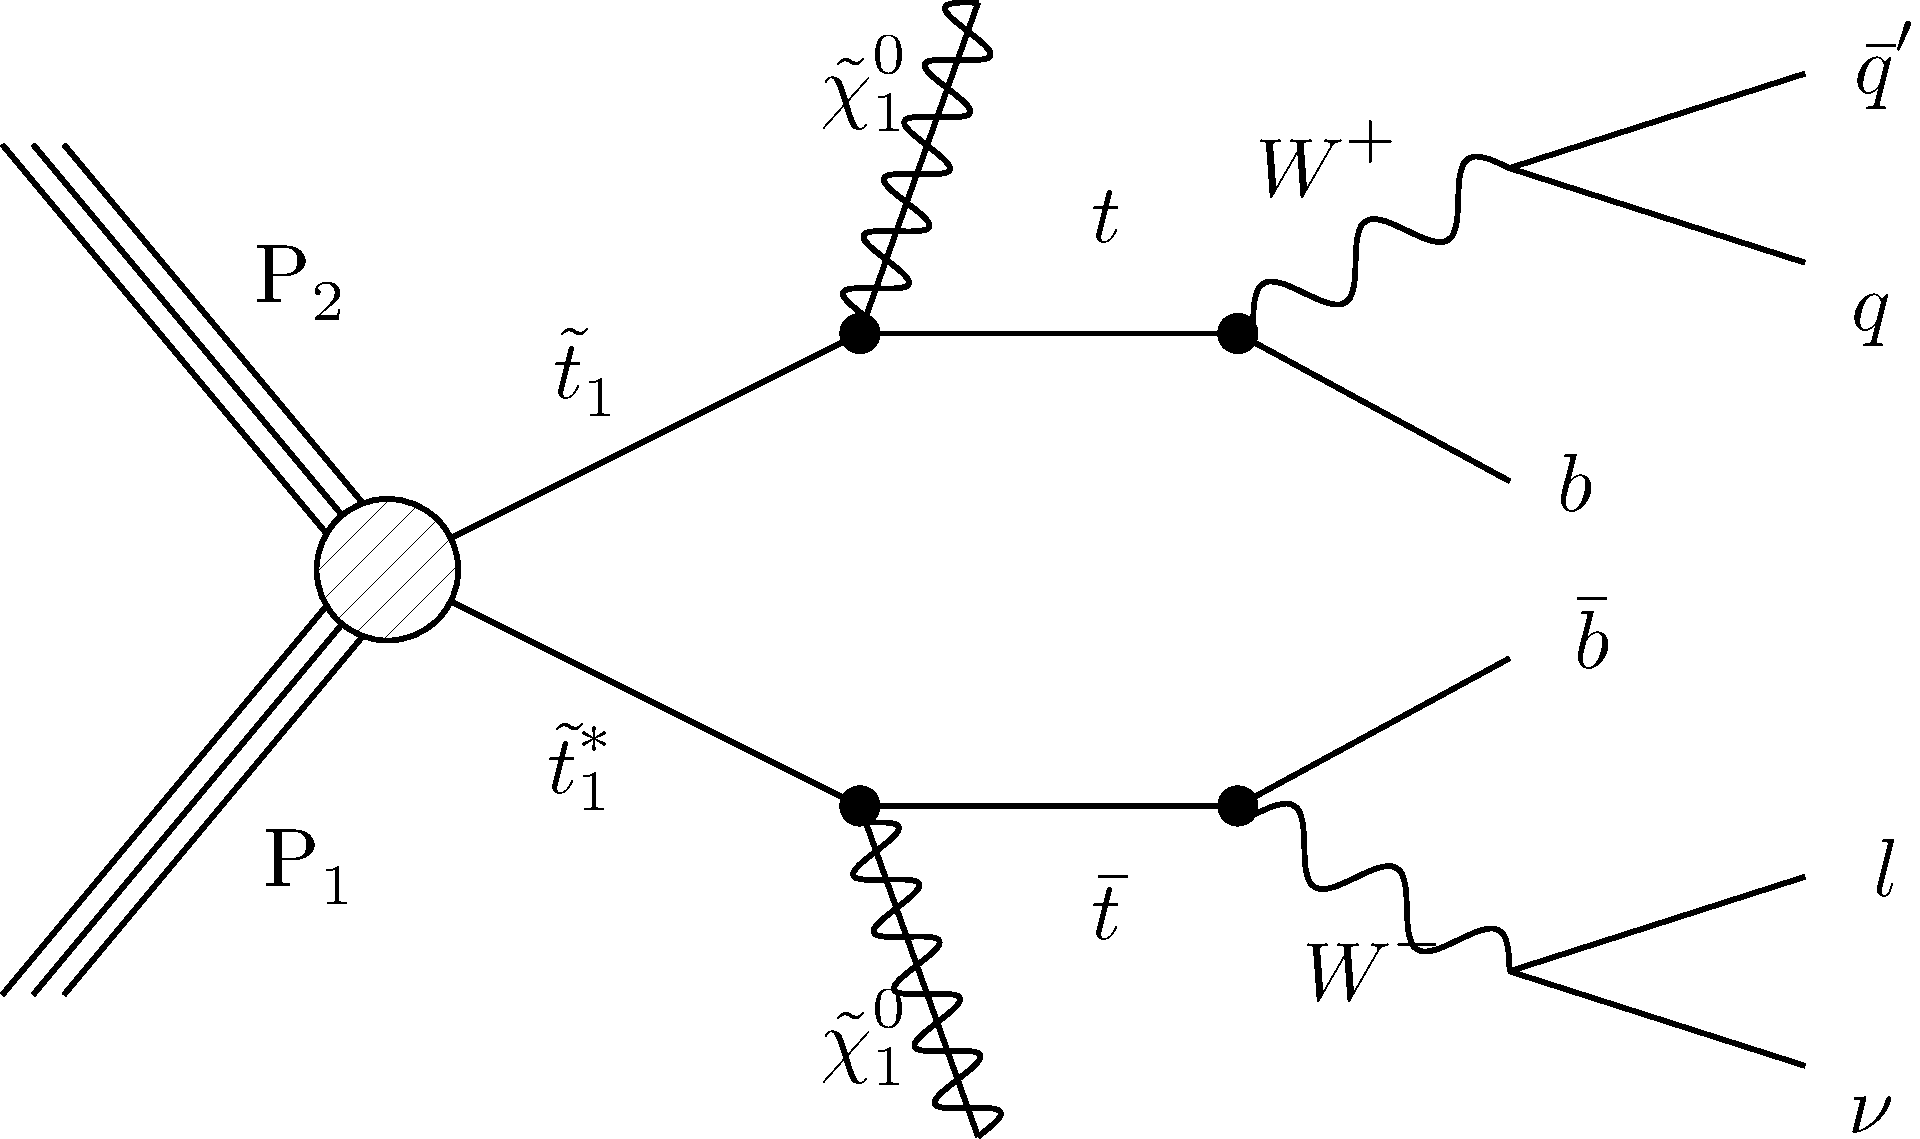
\includegraphics[width=0.45\linewidth]{figures/feynmandiagram_T2tt.pdf}
\includegraphics[width=0.45\linewidth]{figures/feynmandiagram_T2bW.pdf}
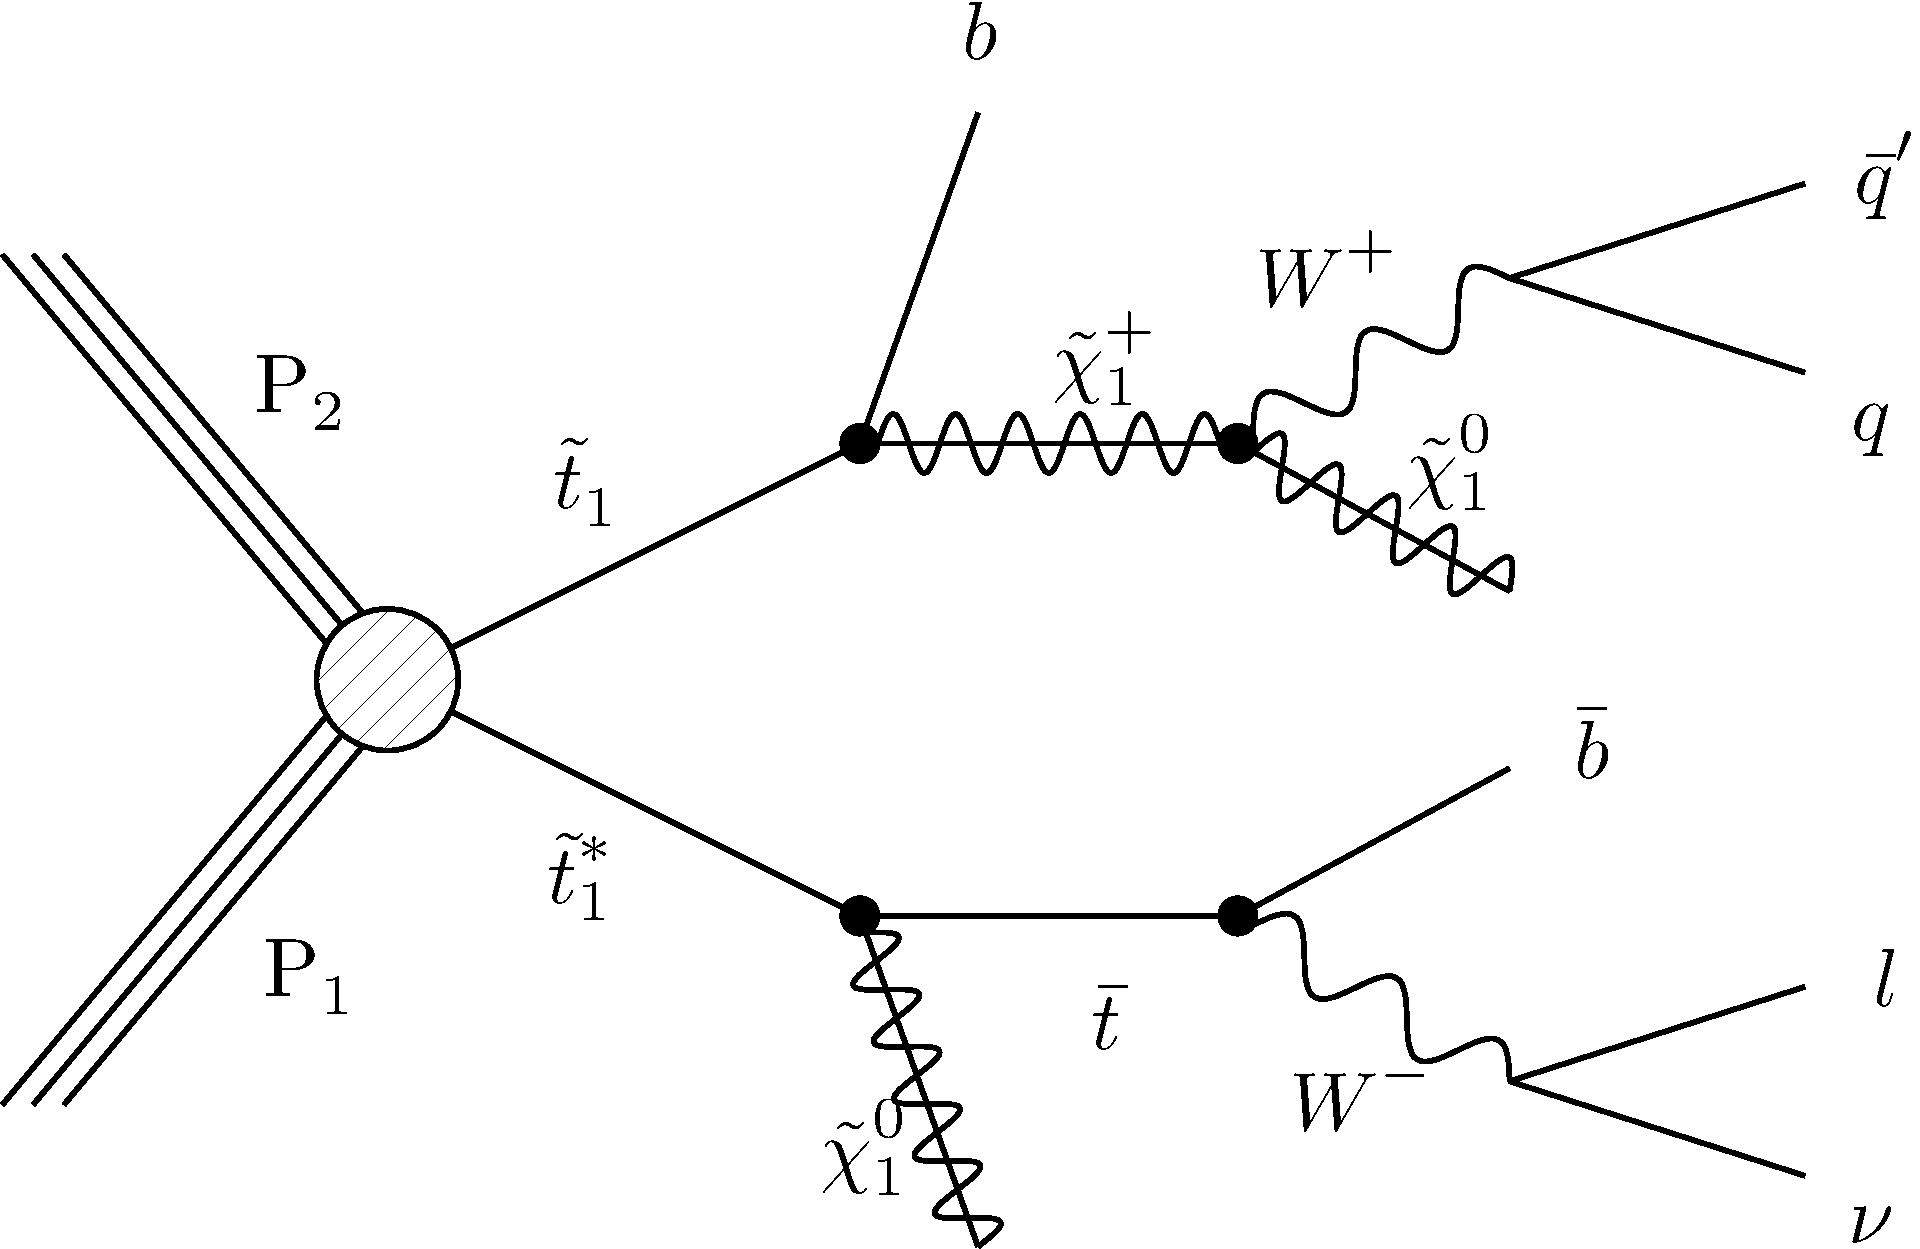
\includegraphics[width=0.45\linewidth]{figures/feynmandiagram_T2tb.pdf}
\caption{Feynman diagrams showing the production of stop pairs that
  subsequently decay to single-lepton final states. Pictured are the
  T2tt, T2bW, and T2tb models, respectively.}
\label{fig:stop:feynmandiagrams}
\end{figure}

\subsection{Compressed T2tt}
\label{ssec:stop:sigcompressed}

There is a region of the $\mstop$ and $\mlsp$ phase space
that is of particular interest to us in this analysis. In the T2tt
model, if the difference between the stop and LSP masses is less than
the mass of the top quark, $\Delta M \lesssim m_t$, then the top quark
must be produced off-shell (i.e. with a mass that is not its normal
$\sim$173 GeV). This kind of process would be difficult to detect
because the production of off-shell top quarks is suppressed, and
because there is also less energy and momentum available to the top
decay products. We may also consider what happens if we go one step
further, to the region where $\mstop - \mlsp \lesssim m_W$. In this case, not
only the top quark but also its resultant W boson must be produced
off-shell, making it even harder to detect this signal. We call these
cases \emph{compressed} T2tt decays, because the phase space available to
the decay products is squeezed down to a small range.

The difficulties in detecting compressed T2tt signals are evident in
the results plot of the Run I analysis \cite{stop1l8tev}. The exclusion
curve for the T2tt model has no coverage in the narrow strip where
$\mstop - \mlsp \approx m_t$, or the strip where $\mstop - \mlsp
\approx m_W$. We call these two regions the \emph{top corridor} and
the \emph{W corridor}, respectively. In this analysis we wished to
fill in these two gaps, and achieve exclusion in the corridor
regions. To that end, I developed a specialized set of
signal regions that target the kinematics of compressed decays, with
the aim of increasing our sensitivity to these signals. These
specialized signal regions will be described in Section
\ref{sec:stop:sigregs}, and the compressed T2tt search will be
described separately from the nominal search in cases where
the two strategies differ.

\section{Datasets and Triggers}
\label{sec:stop:datatrig}

\subsection{Data samples}
\label{ssec:stop:datasamples}

There are two main signatures that we use to search for our stop
decays. The first is, obviously, the presence of a single, isolated lepton.
In addition, all of our signal models have two
LSPs and a neutrino in the final state. The LSPs should go undetected
by the CMS detector, just as neutrinos do, so we also expect our
signals to appear with large amounts of $\met$. % If I move up search strategy, this may no longer be the first place I describe the signature

With these two main signatures in mind, we select our data from the
Single Lepton and $\met$ datasets produced by the CMS
experiment. We also employ the muon+electron dataset for a set of crosscheck
regions to be described in Appendix \ref{apx:stop:emustudies}, and the
single photon datasets for $\met$ resolution studies to be
described in Appendix \ref{apx:stop:metres}. These datasets were recorded during the
2016 datataking period, encompassing eras 2016B through 2016H, and
represent a total integrated luminosity of 35.9 fb\textsuperscript{-1}. Table
\ref{tab:stop:datasets} gives a complete listing of all datasets used
in the analysis.

% Homemade table of datasets goes here. Run ranges collected by hand from DAS.
\begin{table}[htbp]
\centering
\caption{List of CMS datasets used in the single lepton stop search.}
\label{tab:stop:datasets}
\begin{tabular}{|l|r|}
\hline
Dataset & Run Range \\
\hline
  /SingleMuon/Run2016B-03Feb2017\_ver2-v2/MINIAOD     & 273150-275376 \\
  /SingleMuon/Run2016C-03Feb2017-v1/MINIAOD           & 275656-276283 \\
  /SingleMuon/Run2016D-03Feb2017-v1/MINIAOD           & 276315-276811 \\
  /SingleMuon/Run2016E-03Feb2017-v1/MINIAOD           & 276831-277420 \\
  /SingleMuon/Run2016F-03Feb2017-v1/MINIAOD           & 277932-278808 \\
  /SingleMuon/Run2016G-03Feb2017-v1/MINIAOD           & 278820-280385 \\
  /SingleMuon/Run2016H-03Feb2017\_ver2-v1/MINIAOD     & 281613-284035 \\
  /SingleMuon/Run2016H-03Feb2017\_ver3-v1/MINIAOD     & 284036-284044 \\
\hline
  /SingleElectron/Run2016B-03Feb2017\_ver2-v2/MINIAOD & 273150-275376 \\
  /SingleElectron/Run2016C-03Feb2017-v1/MINIAOD       & 275656-276283 \\
  /SingleElectron/Run2016D-03Feb2017-v1/MINIAOD       & 276315-276811 \\
  /SingleElectron/Run2016E-03Feb2017-v1/MINIAOD       & 276831-277420 \\
  /SingleElectron/Run2016F-03Feb2017-v1/MINIAOD       & 277932-278808 \\
  /SingleElectron/Run2016G-03Feb2017-v1/MINIAOD       & 278820-280385 \\
  /SingleElectron/Run2016H-03Feb2017\_ver2-v1/MINIAOD & 281613-284035 \\
  /SingleElectron/Run2016H-03Feb2017\_ver3-v1/MINIAOD & 284036-284044 \\
\hline
  /MET/Run2016B-03Feb2017\_ver2-v2/MINIAOD            & 273150-275376 \\
  /MET/Run2016C-03Feb2017-v1/MINIAOD                  & 275656-276283 \\
  /MET/Run2016D-03Feb2017-v1/MINIAOD                  & 276315-276811 \\
  /MET/Run2016E-03Feb2017-v1/MINIAOD                  & 276831-277420 \\
  /MET/Run2016F-03Feb2017-v1/MINIAOD                  & 277932-278808 \\
  /MET/Run2016G-03Feb2017-v1/MINIAOD                  & 278820-280385 \\
  /MET/Run2016H-03Feb2017\_ver2-v1/MINIAOD            & 281613-284035 \\
  /MET/Run2016H-03Feb2017\_ver3-v1/MINIAOD            & 284036-284044 \\
\hline
  /MuonEG/Run2016B-03Feb2017\_ver2-v2/MINIAOD         & 273150-275376 \\
  /MuonEG/Run2016C-03Feb2017-v1/MINIAOD               & 275656-276283 \\
  /MuonEG/Run2016D-03Feb2017-v1/MINIAOD               & 276315-276811 \\
  /MuonEG/Run2016E-03Feb2017-v1/MINIAOD               & 276831-277420 \\
  /MuonEG/Run2016F-03Feb2017-v1/MINIAOD               & 277932-278808 \\
  /MuonEG/Run2016G-03Feb2017-v1/MINIAOD               & 278820-280385 \\
  /MuonEG/Run2016H-03Feb2017\_ver2-v1/MINIAOD         & 281613-284035 \\
  /MuonEG/Run2016H-03Feb2017\_ver3-v1/MINIAOD         & 284036-284044 \\
\hline
  /SinglePhoton/Run2016B-03Feb2017\_ver2-v2/MINIAOD   & 273150-275376 \\
  /SinglePhoton/Run2016C-03Feb2017-v1/MINIAOD         & 275656-276283 \\
  /SinglePhoton/Run2016D-03Feb2017-v1/MINIAOD         & 276315-276811 \\
  /SinglePhoton/Run2016E-03Feb2017-v1/MINIAOD         & 276831-277420 \\
  /SinglePhoton/Run2016F-03Feb2017-v1/MINIAOD         & 277932-278808 \\
  /SinglePhoton/Run2016G-03Feb2017-v1/MINIAOD         & 278820-280385 \\
  /SinglePhoton/Run2016H-03Feb2017\_ver2-v1/MINIAOD   & 281613-284035 \\
  /SinglePhoton/Run2016H-03Feb2017\_ver3-v1/MINIAOD   & 284036-284044 \\
\hline
\end{tabular}
\end{table}

\subsection{Triggers}
\label{ssec:stop:triggers}

For each of the datasets described above, we select events using
appropriate HLT triggers. Of particular note, we select data events
for our signal regions using the union of the single lepton and $\met$
triggers. This strategy allows us to use leptons that are below their
trigger thresholds, and to compensate for any inefficiency in the
turn-on phase of the $\met$ trigger. The triggers we use are
listed in Table \ref{tab:stop:trigs}.

% Table of HLT triggers paths, adapted from AN-14-463, with a few modifications
\begin{table}[htb]
\caption{HLT trigger paths corresponding to each of the primary
  datasets used in the analysis. The trigger version is suppressed.}
\label{tab:stop:trigs}
\centering
\footnotesize
\begin{tabular}{|l|l|}
\hline
Type & HLT path \\
\hline
SingleMuon & HLT\_Iso(Tk)Mu22 OR HLT\_Iso(Tk)Mu24 \\
SingleElectron & HLT\_Ele25\_eta2p1\_WPTight\_Gsf OR HLT\_Ele27\_eta2p1\_WPTight\_Gsf \\
\hline
\multirow{3}{*}{MET} & HLT\_PFMET170\_HBHECleaned OR \\
 & HLT\_PFMET(NoMu)110\_PFMHT110(NoMu)\_IDTight OR \\
 & HLT\_PFMET(NoMu)120\_PFMHT120(NoMu)\_IDTight \\
\hline
\hline
\multirow{4}{*}{MuonEG} & HLT\_Mu8\_TrkIsoVVL\_Ele23\_CaloIdL\_TrackIdL\_IsoVL(\_DZ) OR \\
 & HLT\_Mu8\_TrkIsoVVL\_Ele17\_CaloIdL\_TrackIdL\_IsoVL\_v* OR \\
 & HLT\_Mu23\_TrkIsoVVL\_Ele12\_CaloIdL\_TrackIdL\_IsoVL(\_DZ) OR \\
 & HLT\_Mu17\_TrkIsoVVL\_Ele12\_CaloIdL\_TrackIdL\_IsoVL\_v* \\
\hline
\multirow{2}{*}{SinglePhoton} & HLT\_Photon*\_R9Id90\_HE10\_IsoM OR HLT\_Photon165\_HE10 OR \\
 & HLT\_Photon175 OR HLT\_Photon250\_NoHE \\
\hline
\end{tabular}
\end{table}

\subsection{Trigger Efficiency Measurements}
\label{ssec:stop:trigeff}

We measure the efficiency of our combined single lepton and $\met$
triggers in a sample of events from the JetHT primary dataset,
selected using the \verb+HLT_(PF)HT*+ trigger paths. We use events
triggered on $H_T$ because this trigger is expected to be orthogonal
to the $\met$ and lepton $p_T$ triggers, allowing us to examine the full
spectrum of these variables. The trigger
efficiency is parameterized in $\met$ and lepton $p_T$. We select events
with at least one lepton and two jets. Our definitions of leptons,
jets, and $\met$ are presented later, in Section
\ref{sec:stop:selections}. For any given bin in the efficiency
histogram, the efficiency is computed as the number of events in that
bin passing our triggers divided by the total number of events in that
bin.

Figure \ref{fig:stop:trigeff:1lepmet} shows the parameterized trigger
efficiencies, separated by flavor of the leading lepton. Using 35.9 fb\textsuperscript{-1}
of data, our overall trigger efficiency is 99.1\% in the region $\met >$
250 GeV and lepton $p_T >$ 20 GeV. Because this efficiency is so close
to 100\%, we do not correct for the small inefficiency. However, we
assign a systematic uncertainty of 2\% for events with $\met$ below 300
GeV, and 4\% for events with $\met$ greater than 300 GeV.

% Plots of trigger efficiency taken from AN-16-463.
\begin{figure}[htb]
\centering
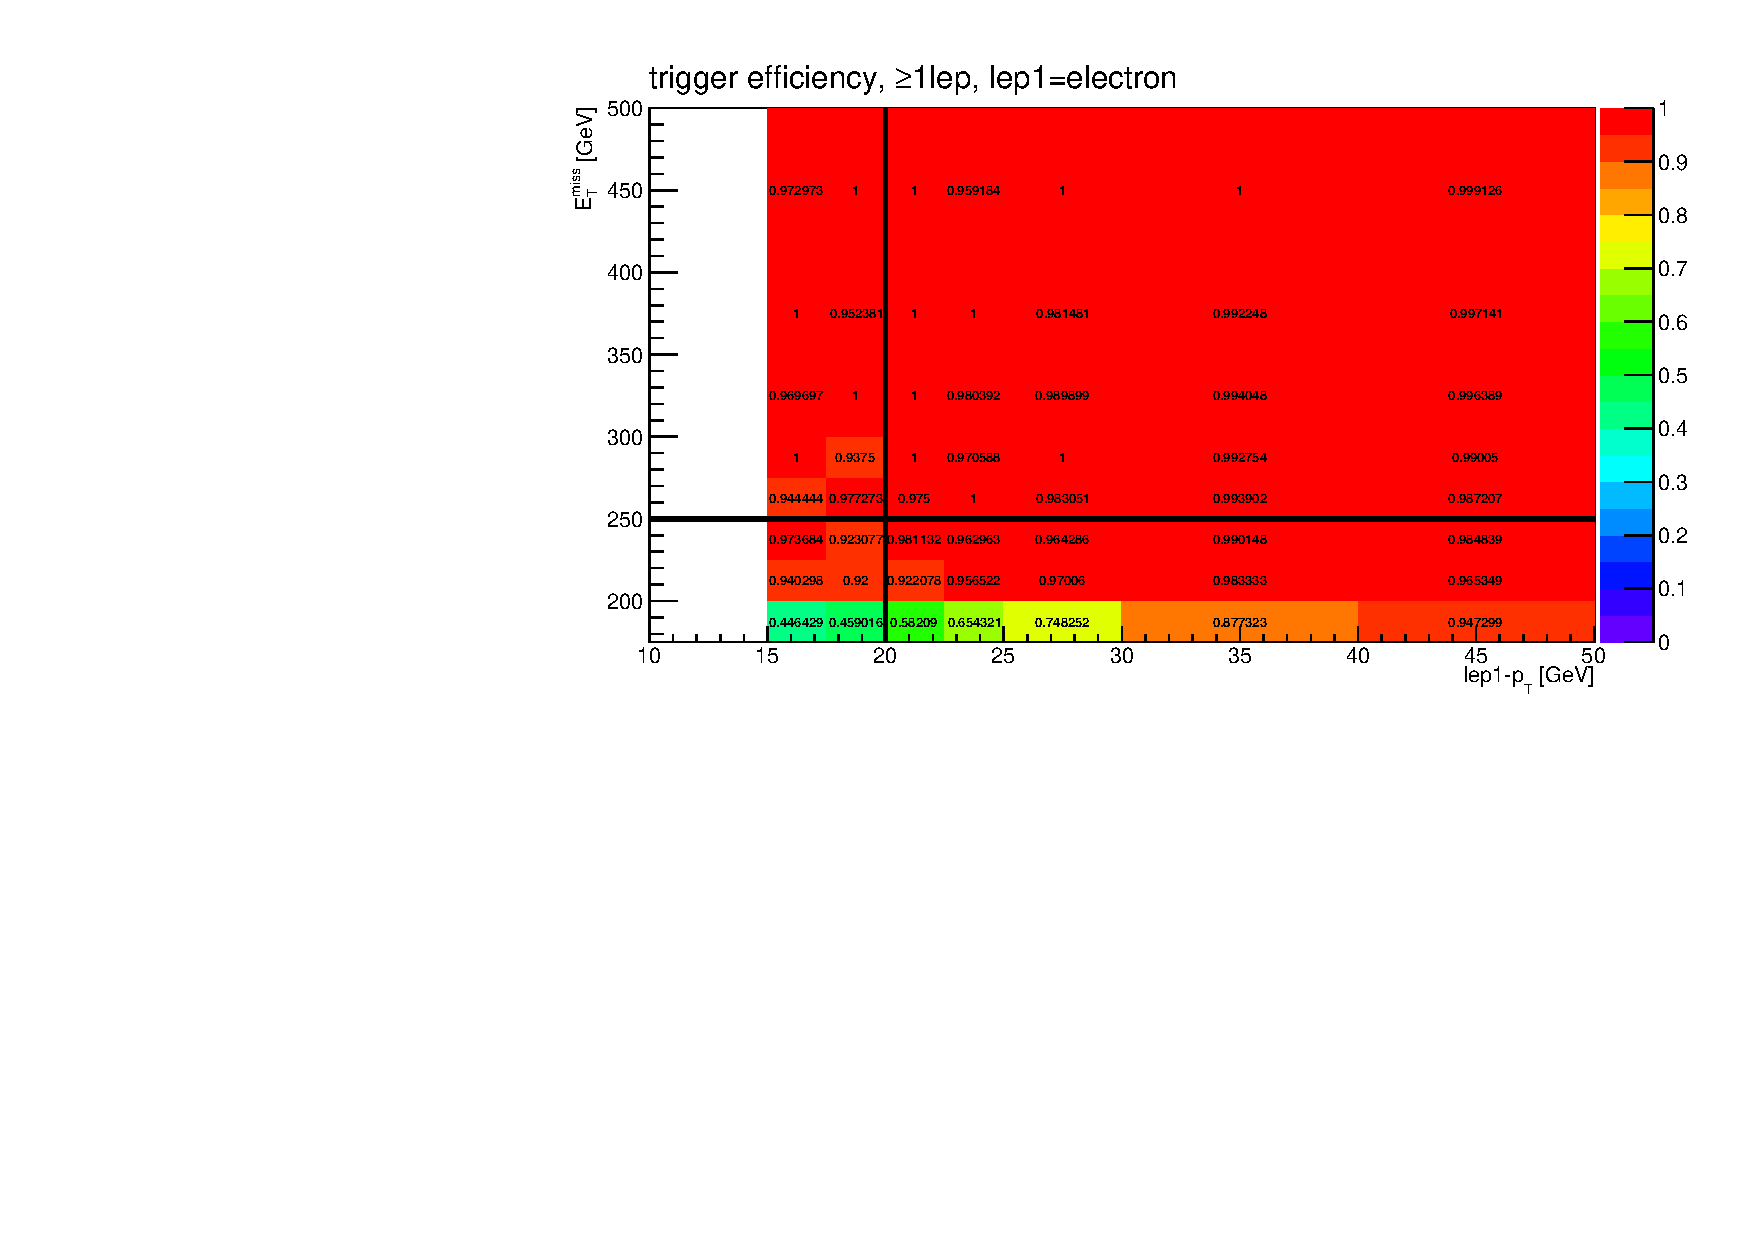
\includegraphics[width=0.45\textwidth]{figures/TriggerEff_el.pdf}
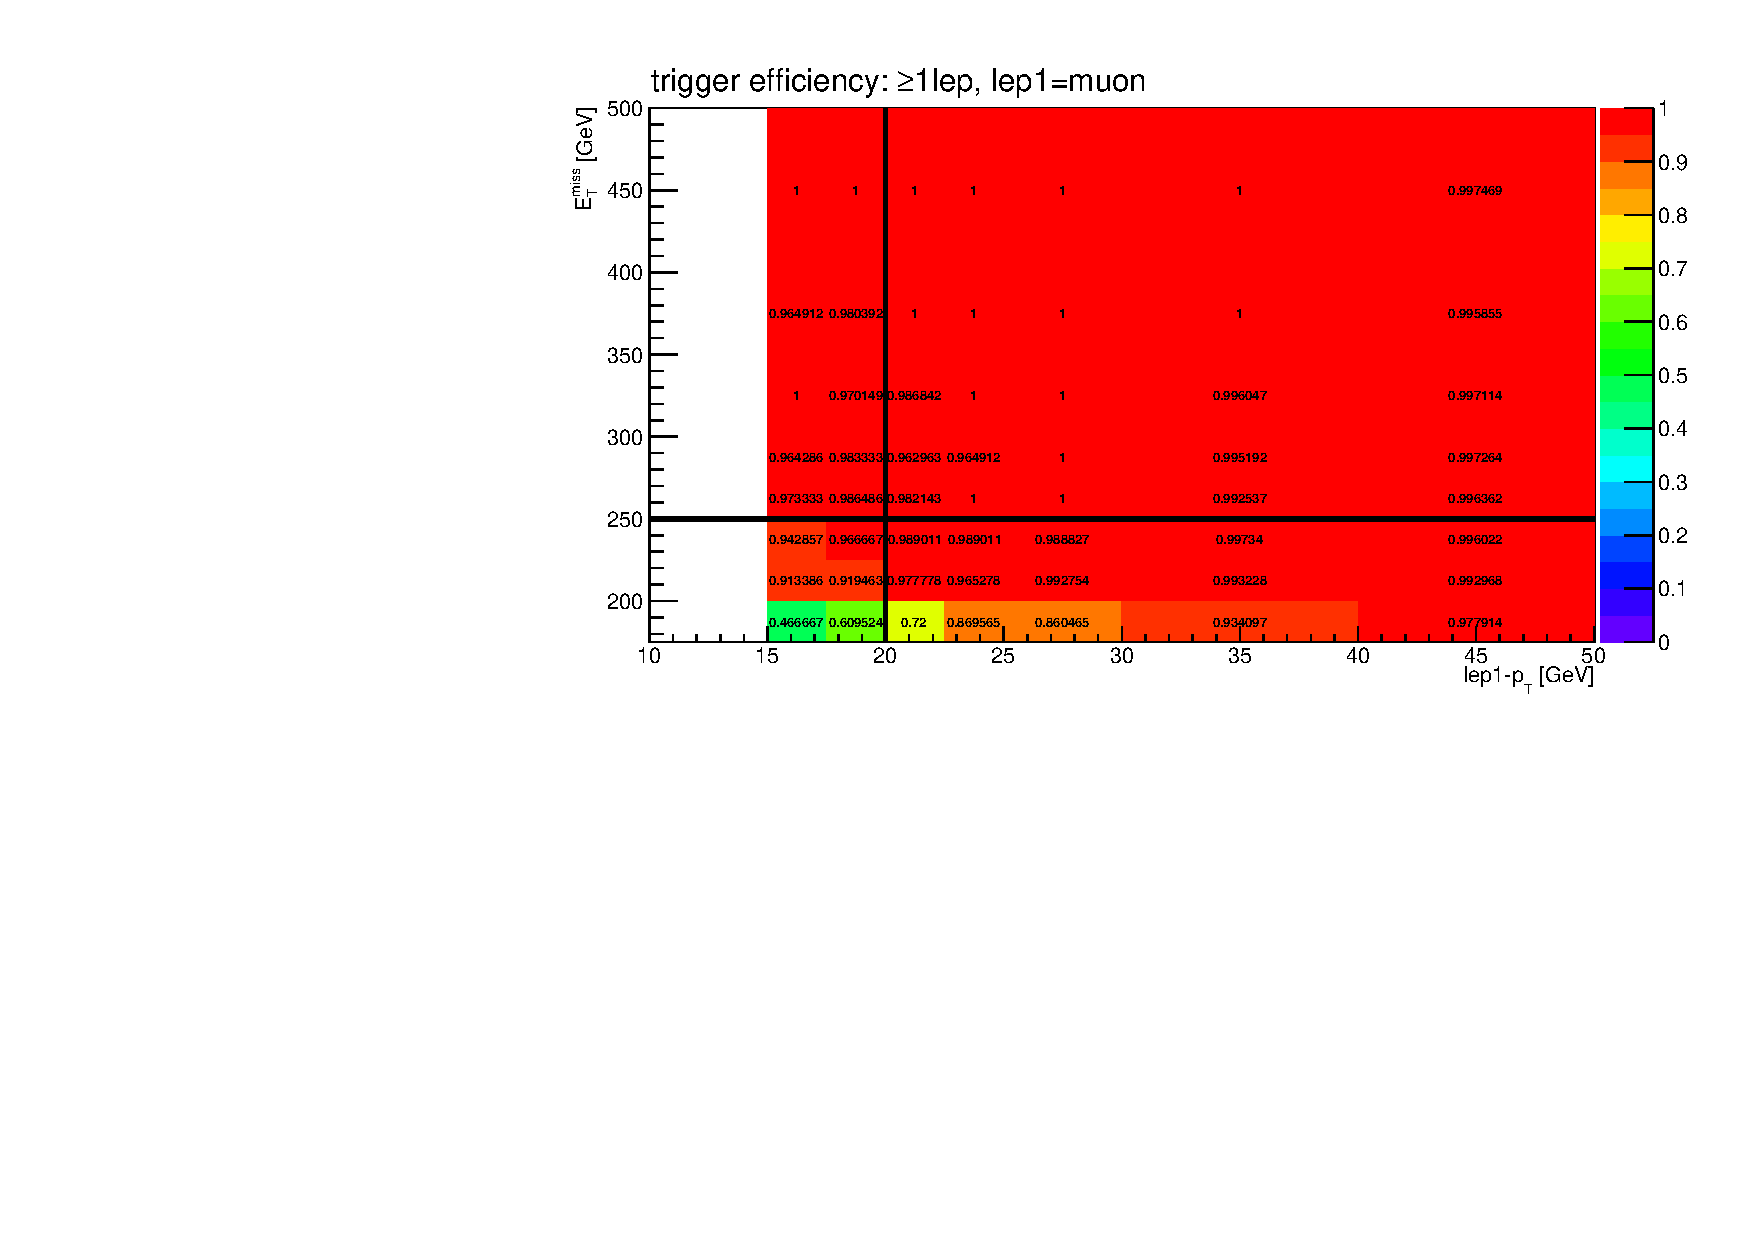
\includegraphics[width=0.45\textwidth]{figures/TriggerEff_mu.pdf}
\caption{Measured efficiencies for the union of the single lepton and
  $\met$ triggers. Efficiency is represented by the z-axis color scale. The
  efficiencies are presented separately for the case where the leading
  lepton is an electron (left), and a muon (right).}
\label{fig:stop:trigeff:1lepmet}
\end{figure}

% It kinda helps to know what the lost lepton background is before
% this part
As Section \ref{ssec:stop:lostlep} will describe, if we fail to
reconstruct a second lepton, the $p_T$ of that lepton effectively
contributes to the $\met$ of the event. When considering such events, we must
re-evaluate the efficiency of our combined single lepton and $\met$
triggers. We do so using the exact same procedures described above,
except that we additionally require events to have a second lepton
with $p_T >$ 10 GeV. These efficiencies are presented in Figure
\ref{fig:stop:trigeff:2ndlepplusmet}. Because the combined triggers
have substantial inefficiency at low $\met$ and low lepton $p_T$, we
do correct our Monte Carlo simulations for these trigger
efficiencies when performing this background estimation.

% Plots of 2nd-lep-plus-met trigger efficiency taken from AN-16-463.
\begin{figure}[htb]
\centering
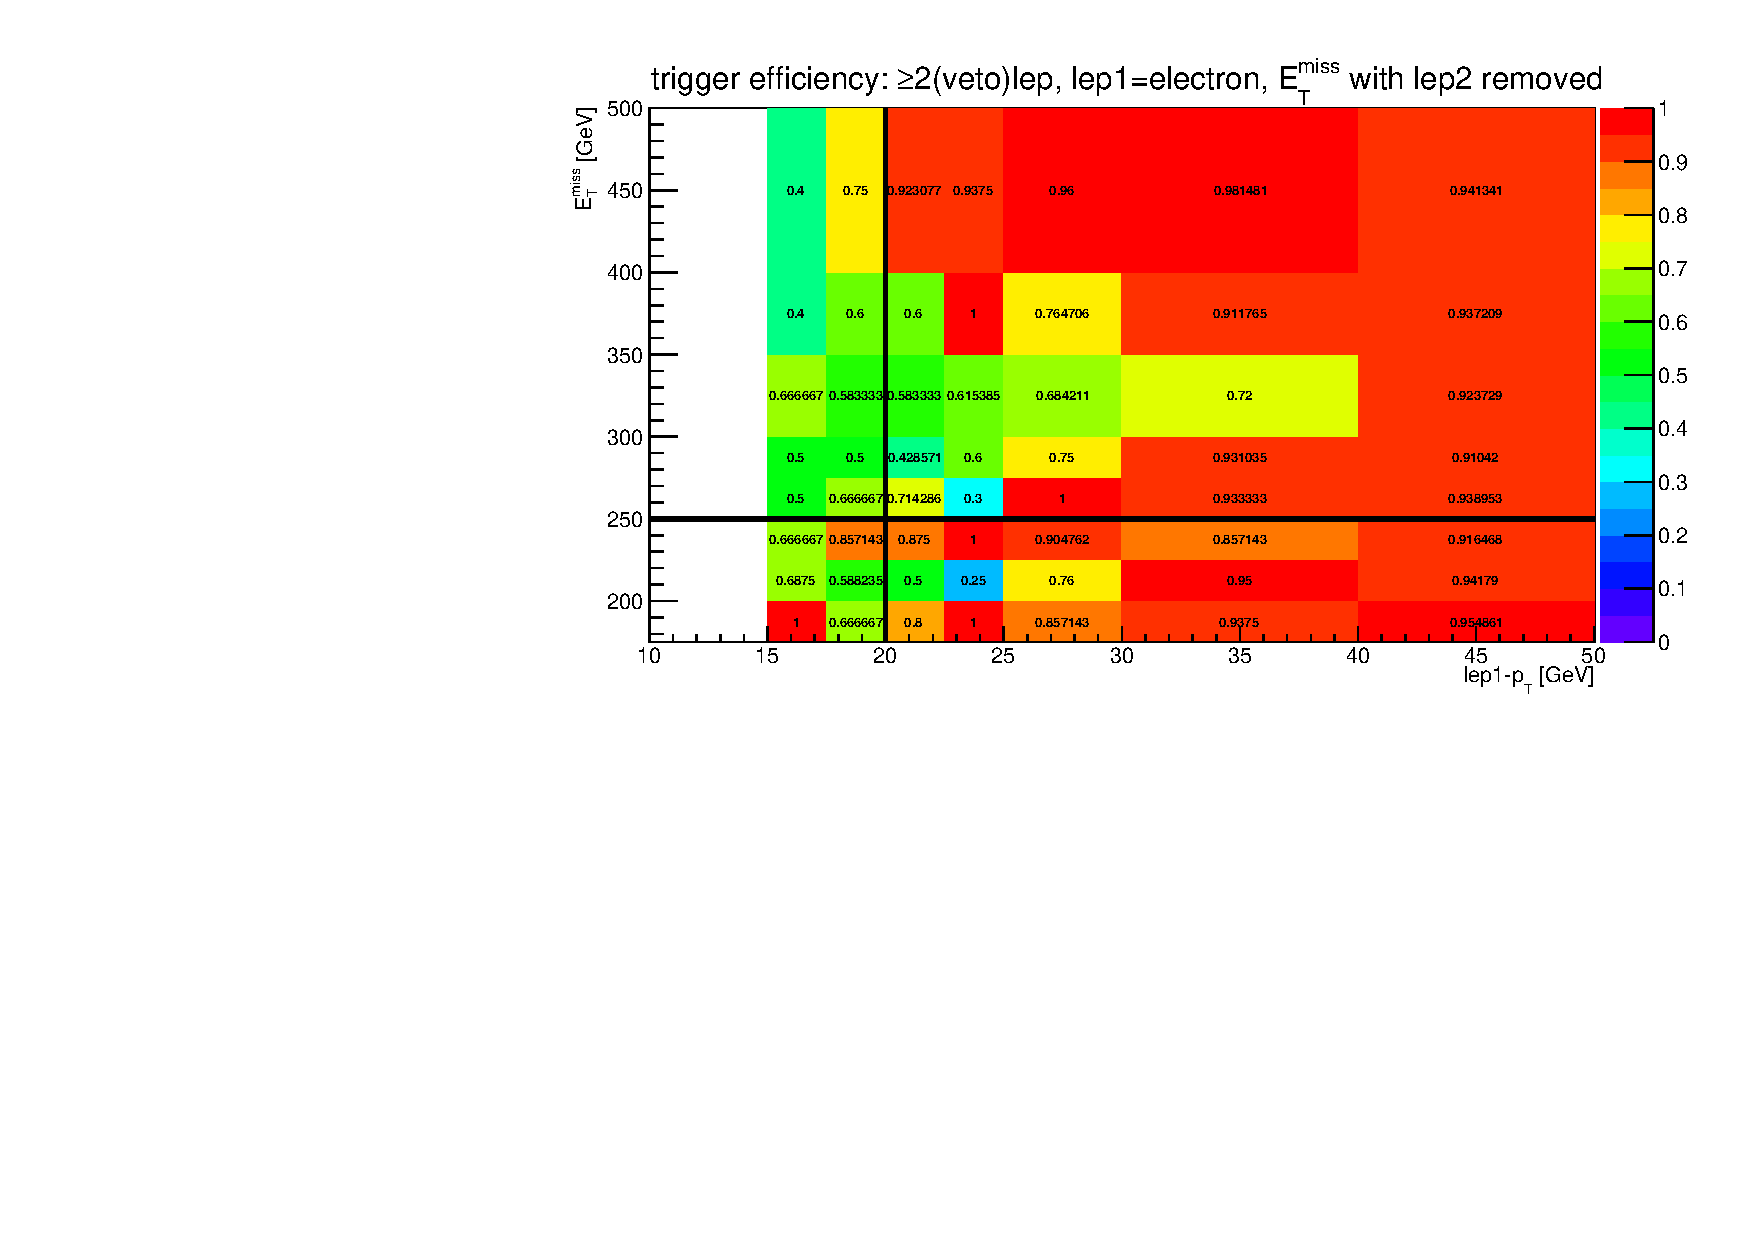
\includegraphics[width=0.45\textwidth]{figures/TriggerEff2l_el.pdf}
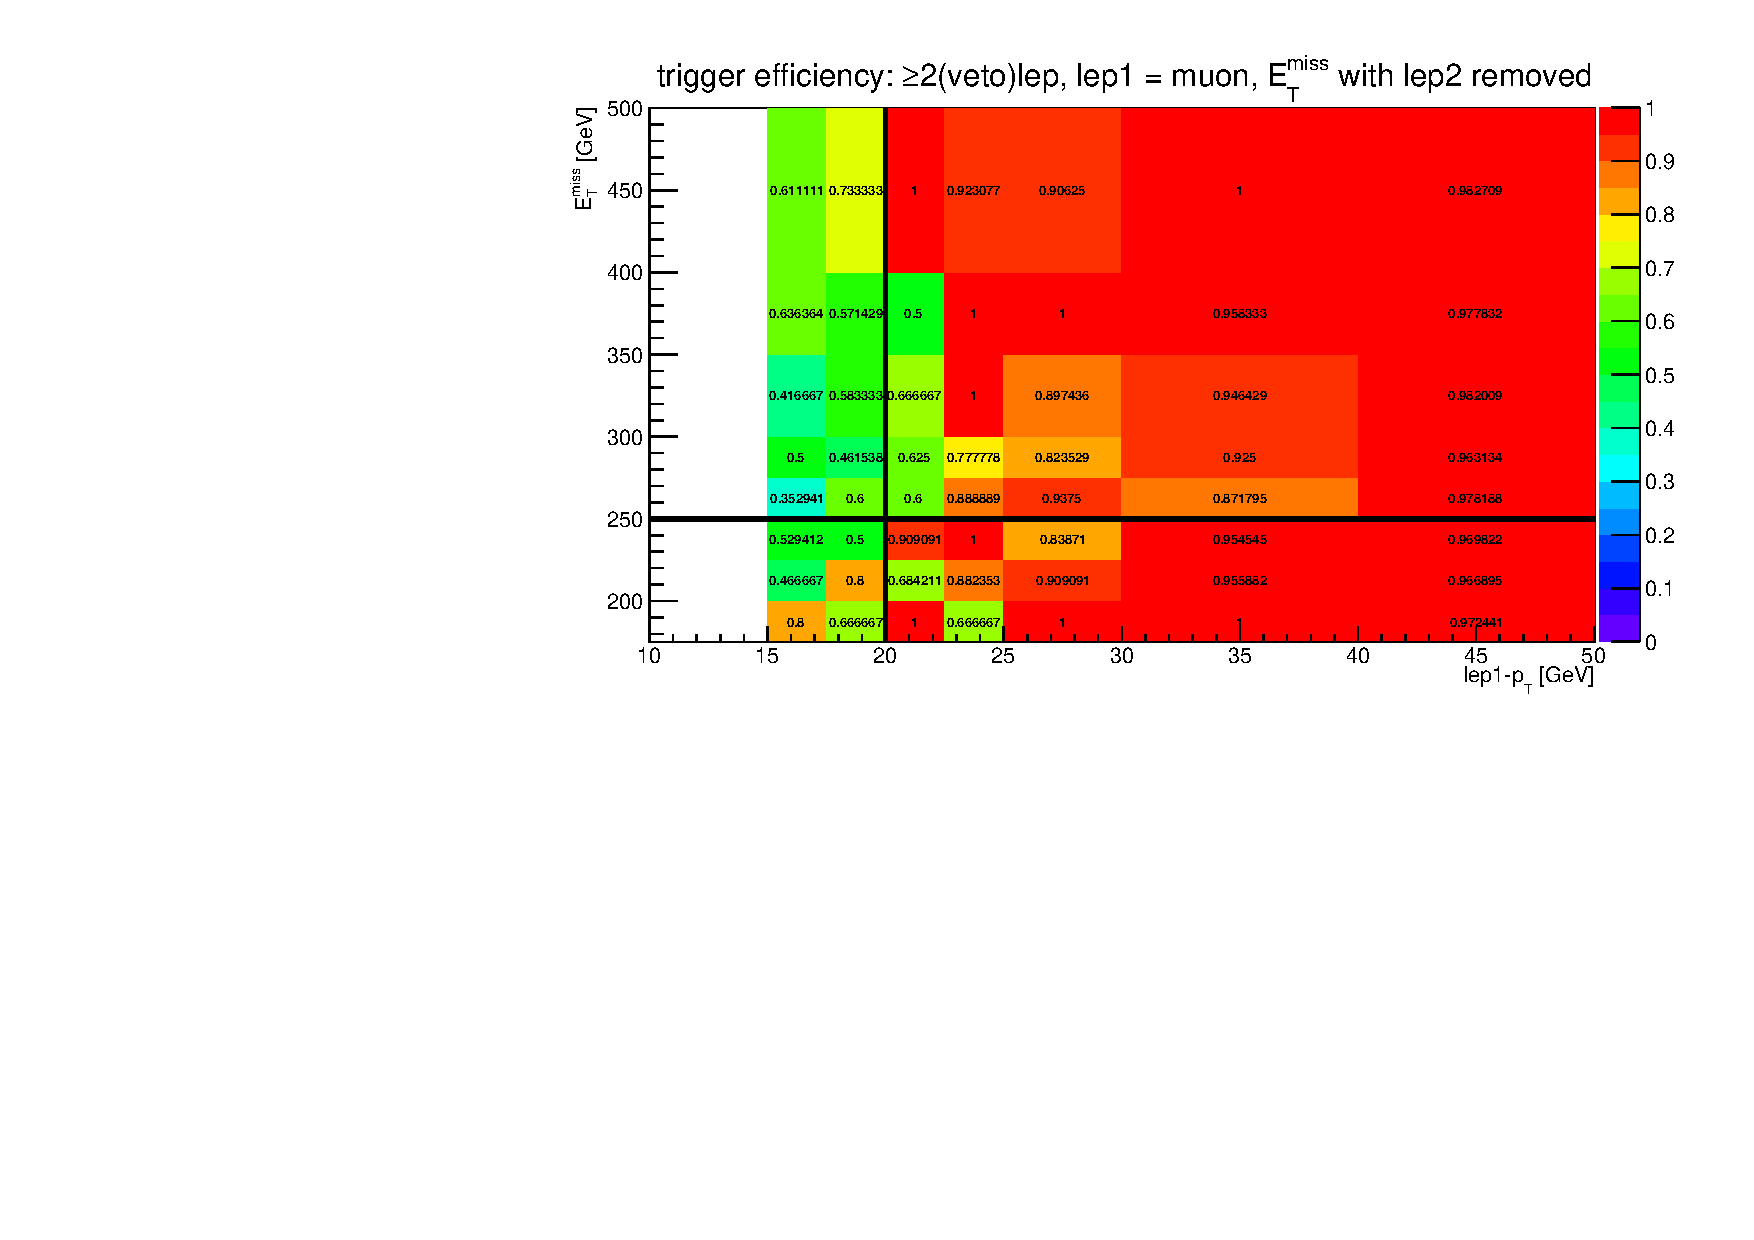
\includegraphics[width=0.45\textwidth]{figures/TriggerEff2l_mu.pdf}
\caption{Measured efficiencies for the union of the single lepton and
  $\met$ triggers, when the sub-leading lepton $p_T$ is added to the
  $\met$. Efficiency is represented by the z-axis color scale. The
  efficiencies are presented separately for the case where
  the leading lepton is an electron (left), and a muon (right).}
\label{fig:stop:trigeff:2ndlepplusmet}
\end{figure}

\subsection{Monte Carlo Samples}
\label{ssec:stop:mcsamples}

Our analysis relies on modeling a number of background and signal
processes using Monte Carlo simulation. Table \ref{tab:stop:mcsamples}
presents the complete list of Monte Carlo samples used. All samples
are produced as MINIAODSIM. Our SM samples were made using FullSim,
while the SUSY signal samples were made using FastSim \cite{fastsim}.

% Table of MC samples taken from AN-16-463.
\begin{table}[htp]
\caption[Monte Carlo simulation datasets used in this analysis, and
  their theoretical cross sections. The symbols * and $\dagger$ replace
  longer strings.]
  {Monte Carlo simulation datasets used in this analysis, and their
  theoretical cross sections. The symbol * replaces the string
  RunIISummer16MiniAODv2-PUMoriond17\_80X\_mcRun2\_asymptotic\_2016\_TrancheIV\_v6, % Warning: underfull hboxes abound here!
  and the $\dagger$ replaces
  RunIISpring16MiniAODv2-PUSpring16Fast\_80X\_mcRun2\_asymptotic\_2016\_miniAODv2\_v0.}
\label{tab:stop:mcsamples}
\centering
{\footnotesize
\begin{tabular}{|l|c|c|c|}
\hline
Sample & Cross Section \\
& [pb] \\
\hline
/TTJets\_SingleLeptFromT\_TuneCUETP8M1\_13TeV-madgraphMLM-pythia8/*(\_ext)-v1 & 182.7 \\
/TTJets\_SingleLeptFromTbar\_TuneCUETP8M1\_13TeV-madgraphMLM-pythia8/*(\_ext)-v1 & 182.7 \\
/TTJets\_DiLept\_TuneCUETP8M1\_13TeV-madgraphMLM-pythia8/*\_ext-v1 (and *-v4) & 87.3 \\
/ST\_tW\_top\_5f\_NoFullyHadronicDecays\_13TeV-powheg\_TuneCUETP8M1/*-v1 & 19.6 \\
/ST\_tW\_antitop\_5f\_NoFullyHadronicDecays\_13TeV-powheg\_TuneCUETP8M1/*-v1 & 19.6 \\
/ST\_t-channel\_top\_4f\_leptonDecays\_13TeV-powheg-pythia8\_TuneCUETP8M1/*-v1 & 44.1 \\
/ST\_t-channel\_antitop\_4f\_leptonDecays\_13TeV-powheg-pythia8\_TuneCUETP8M1/*-v1 & 26.2 \\
/ST\_s-channel\_4f\_leptonDecays\_13TeV-amcatnlo-pythia8\_TuneCUETP8M1/*-v1 & 3.7 \\
/W1JetsToLNu\_TuneCUETP8M1\_13TeV-madgraphMLM-pythia8/*-v1 & 11782  \\
/W2JetsToLNu\_TuneCUETP8M1\_13TeV-madgraphMLM-pythia8/*-v1 & 3841 \\
/W3JetsToLNu\_TuneCUETP8M1\_13TeV-madgraphMLM-pythia8/*-v1 & 1160 \\
/W4JetsToLNu\_TuneCUETP8M1\_13TeV-madgraphMLM-pythia8/*-v1 & 600 \\
/W1JetsToLNu\_NuPt-200\_TuneCUETP8M1\_13TeV-madgraphMLM-pythia8/*-v1 & 2.36  \\
/W2JetsToLNu\_NuPt-200\_TuneCUETP8M1\_13TeV-madgraphMLM-pythia8/*-v1 & 4.95 \\
/W3JetsToLNu\_NuPt-200\_TuneCUETP8M1\_13TeV-madgraphMLM-pythia8/*-v1 & 4.94 \\
/W4JetsToLNu\_NuPt-200\_TuneCUETP8M1\_13TeV-madgraphMLM-pythia8/*-v1 & 8.83 \\
/ttWJets\_13TeV\_madgraphMLM/*-v1 & 0.61 \\
/ttZJets\_13TeV\_madgraphMLM/*-v1 & 0.78 \\
/WWTo2L2Nu\_13TeV-powheg/*-v1 & 12.18 \\
/WWToLNuQQ\_13TeV-powheg/*-v1 & 50.00  \\
/WZTo3LNu\_TuneCUETP8M1\_13TeV-powheg-pythia8/*-v1 & 4.43 \\
/WZTo2L2Q\_13TeV\_amcatnloFXFX\_madspin\_pythia8/*-v1 & 5.60 \\
/WZTo1L1Nu2Q\_13TeV\_amcatnloFXFX\_madspin\_pythia8/*-v1 & 10.74 \\
/WZTo1L3Nu\_13TeV\_amcatnloFXFX\_madspin\_pythia8/*-v1 & 3.05 \\
/ZZTo4L\_13TeV\_powheg\_pythia8/*-v1 & 1.25 \\
/ZZTo2L2Q\_13TeV\_amcatnloFXFX\_madspin\_pythia8/*-v1 & 3.22 \\
/ZZTo2L2Nu\_13TeV\_powheg\_pythia8/*-v1 & 0.56 \\
/ZZTo2Q2Nu\_13TeV\_amcatnloFXFX\_madspin\_pythia8/*-v1 & 4.73 \\
/SMS-T2tt\_mStop-150to250\_TuneCUETP8M1\_13TeV-madgraphMLM-pythia8/$\dagger$-v1 & \\
/SMS-T2tt\_mStop-250to350\_TuneCUETP8M1\_13TeV-madgraphMLM-pythia8/$\dagger$-v1 & \\
/SMS-T2tt\_mStop-350to400\_TuneCUETP8M1\_13TeV-madgraphMLM-pythia8/$\dagger$-v1 & \\
/SMS-T2tt\_mStop-400to1200\_TuneCUETP8M1\_13TeV-madgraphMLM-pythia8/$\dagger$-v1 & \\
/SMS-T2bW\_TuneCUETP8M1\_13TeV-madgraphMLM-pythia8/$\dagger$-v1 & \\
/SMS-T2bt\_TuneCUETP8M1\_13TeV-madgraphMLM-pythia8/$\dagger$-v1 & \\
\hline
\end{tabular}
}
\end{table}

\section{Search Strategy}
\label{sec:stop:searchstrategy}

Because we are searching for single lepton stop decays, we must select
events with one and only one lepton in them. In addition, the LSPs and
charginos should go undetected by the CMS detector; those sparticles
plus the neutrino should give relatively
large amounts of $\met$. Therefore, our main experimental signature is a
single lepton plus high $\met$.

Many other physics processes can produce a single lepton plus high
$\met$, or can produce signatures that resemble these. We must therefore
identify these backgrounds, and attempt to reduce their presence using
a series of cuts and selections. When it is not possible to mitigate
the backgrounds with cuts, we must attempt to estimate how many
background events fall into our signal regions so we can exclude them
from the final calculations.

In the absence of any particular cuts and selections, the largest
background will naturally be SM processes that produce one true lepton
and large $\met$. The notable example is $\ttonelep$,
though other processes contribute as well, such as W-boson production
with jets, where the W decays leptonically. In order to combat this
background component, we first add a cut on the transverse mass of the
lepton plus the $\met$, or $\mt$. The exact formula for this variable is
given by Equation \ref{eq:stop:mt} in Section \ref{ssec:stop:mt}. This cut works in
concert with our high-$\met$ requirement to help reduce the single-lepton
background component.

% M_T study plots adapted from AN-16-463.
\begin{figure}[htb]
\centering
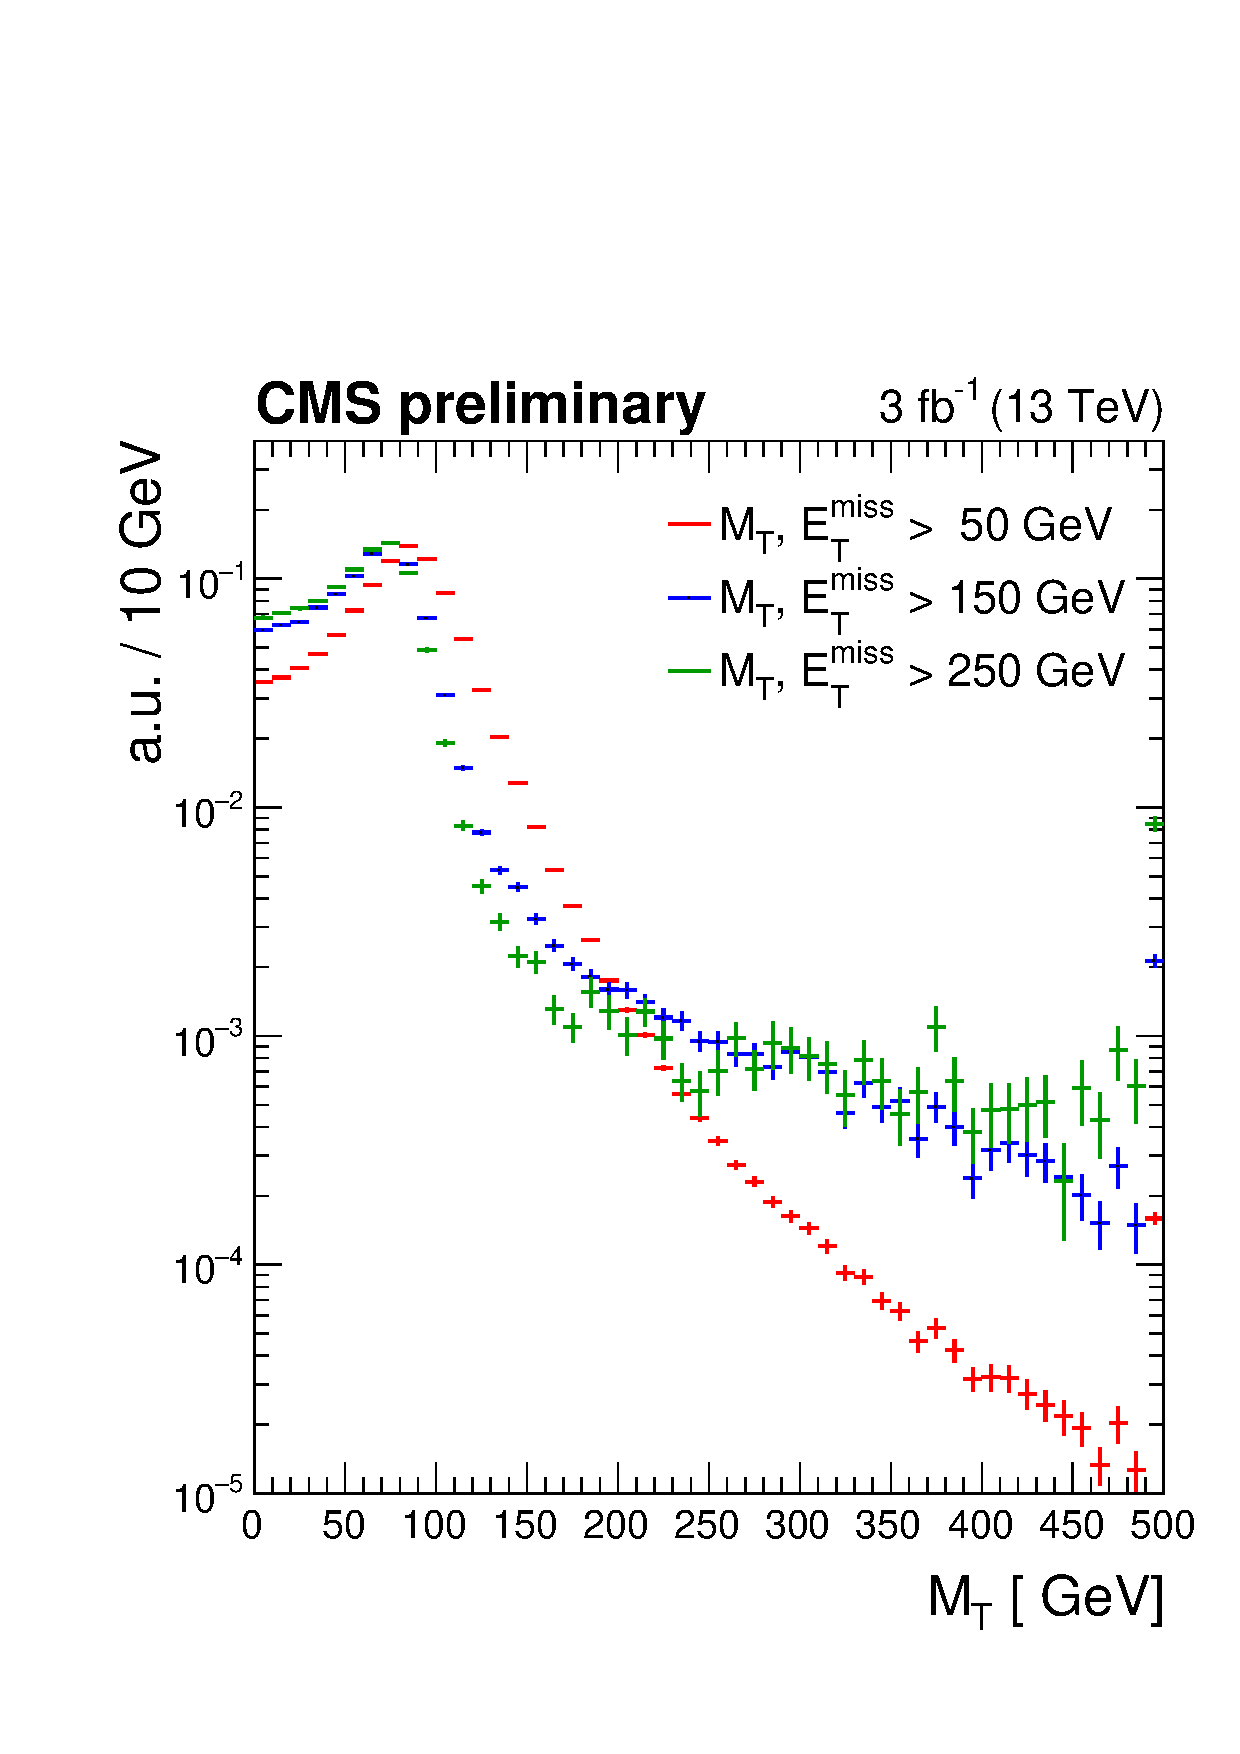
\includegraphics[width=0.45\textwidth]{figures/mtstudies_W_reco.pdf}
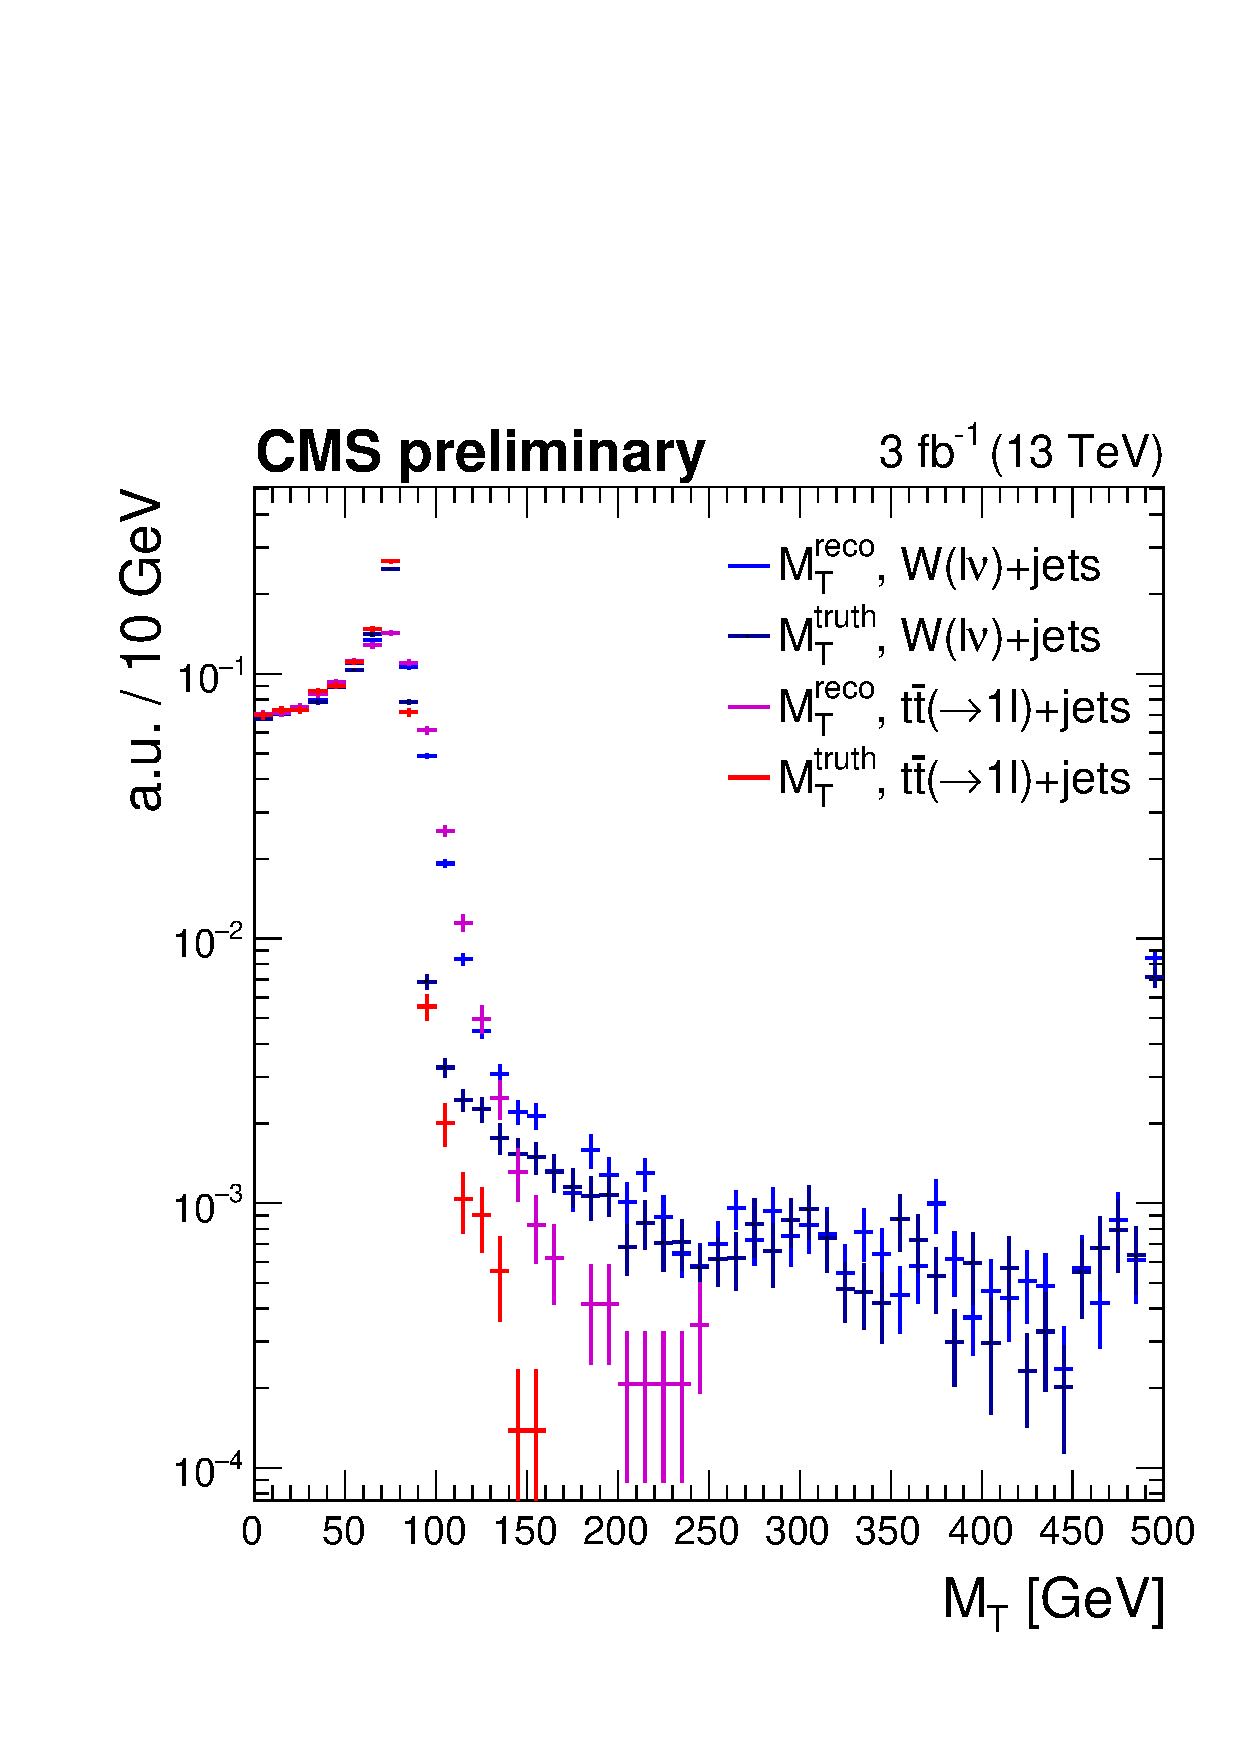
\includegraphics[width=0.45\textwidth]{figures/mtstudies_WTop_recogen.pdf}
\caption{$\mt$ distributions in W+jets with various $\met$ selections
  applied, and comparison between gen and reco $\mt$ in W+jets and
  $\ttonelep$.}
\label{fig:stop:mtstudies}
\end{figure}

Figure \ref{fig:stop:mtstudies} shows the results of several
investigations into the $\mt$ variable. The left plot shows the
reconstructed value of $\mt$ in a sample of W($\ell\nu$)+jets MC
events, with three different $\met$ cuts applied. As the plot shows,
higher $\met$ requirements cause the W-boson mass edge to become more
sharply defined, making it easier to set a cut threshold.

The right plot shows generator-level $\mt$ and reconstructed $\mt$
for both W+jets and $\ttonelep$ simulated events. These
events were selected by requiring a single lepton and at least 2
jets, all with $p_T > 30$ GeV, and $\met >$ 250 GeV. The generator-level $\mt$ was
calculated using the neutrino momentum in place of the $\met$. The plot
shows that the tails of the $\mt$ distribution look very different for
W+jets and $\ttonelep$. In the case of $\ttonelep$, the top mass
restricts the mass spectrum of the W-boson, so that most events in the
tail are present because of the limited resolution of $\met$
reconstruction. This is seen in the difference between the gen and reco
$\mt$ spectra. By contrast, in W+jets events, there is no constraint
on the W mass, so the tail is attributable to the natural width of the
W-boson mass spectrum. Thus, by selecting an appropriate $\mt$ cut, we
can effectively reduce the single lepton background to mostly W+jets
events. We can then estimate the size of the remaining background
component using techniques that will be described in Sections
\ref{ssec:stop:1lw} and \ref{ssec:stop:1ltop}.

After reducing the single lepton background using $\met$ and $\mt$ cuts,
the next largest background comes from events with two genuine
leptons, such as $\ttdilep$, where one of the leptons is not
reconstructed. As Section \ref{sec:stop:selections} will describe, we
veto events that have a second electron, muon, or tau, as well as
events with an isolated track in them. Nevertheless, these vetos are
not perfect. And often, a second lepton falls outside our range of
acceptance in $p_T$ or $\eta$, is not isolated, or is not
reconstructed. We call this component the ``lost lepton''
background. As Chapter \ref{chap:afb} has demonstrated, we have a good
understanding of the $\ttdilep$ process, and can model it fairly
well. On the basis of that strong understanding, we estimate this
background using data-driven techniques described in Section
\ref{ssec:stop:lostlep}.

The final background to consider is events with one genuine lepton,
but where the high $\met$ comes from a $Z \rightarrow \nu\nu$ decay,
and not from SUSY particles. The largest contributor to this
background is $ttZ$ events, where the $\ttbar$ pair decays
semileptonically and the Z decays to invisible neutrinos; the next
largest contributor is WZ production. There is little we can do to
exclude such events with cuts; fortunately, this background component
is relatively small. We estimate the $Z \rightarrow \nu\nu$
component using MC with theoretical uncertainties applied, as
described in Section \ref{ssec:stop:rarebkg}.

\section{Object and Event Selection}
\label{sec:stop:selections}

We define our physics objects, and use them to select events, with an
eye to maximizing our acceptance of SUSY signals, while rejecting SM backgrounds.

\subsection{Vertex Selections}
\label{ssec:stop:vtxselections}

For an event to be selected, at least the first vertex in the event
must be a good vertex. A vertex is considered to be ``good'' if it
meets the following criteria:

\begin{itemize}
\item The tracks used to create the vertex must have trajectory fits
  with positive $\chi^2$ values.
\item The vertex fit must have at least 5 degrees of freedom.
\item The distance between the vertex and the nominal center of the
  detector must have a $z$-component of less than 24 cm.
\item The same distance must have a transverse component, $\rho$, of
  less than 2 cm.
\end{itemize}

If multiple vertices in an event meet these criteria, we choose the
one whose associated tracks have the highest $\sum p_T^2$ to be our
primary vertex (PV), from which all of our physics objects originate.

\subsection{Lepton Selections and Veto}
\label{ssec:stop:lepselections}

We select events that have one well-identified reconstructed lepton
(electron or muon), and veto events with additional leptons. All our
identification criteria are based on the POG recommendations, and are
described in Table \ref{tab:stop:lepselections}.

For our electrons, we remove the POG-recommended isolation cut, and
substitute a cut based on \emph{relative mini-isolation}, as is standard for
SUSY searches at CMS. Relative mini-isolation is defined as the sum of
the $p_T$ of the particle flow candidates within a cone-shaped region
around the lepton, where the cone size varies with the lepton
$p_T$. For lepton $p_T <$ 50 GeV, the cone size is 0.2 in $\Delta
R$. For $p_T$ between 50 and 200 GeV, the cone size is defined to be
10.0 GeV / $p_T^{\text{lep}}$. Finally, for lepton $p_T$ above 200 GeV, the
cone size is fixed at 0.05. The rationale for reducing the cone size
as lepton $p_T$ rises is to avoid vetoing signal events
where a boosted top decays to a lepton and b-jet that are nearly
colinear. Pileup correction is performed using the average energy
density in the event, and the same effective area used in the
mini-isolation calculation.

\begin{table}[htb]
\centering
\caption{Criteria used to identify electrons or muons. We select
  exactly one good lepton, and veto any additional leptons, using two
  different sets of criteria.}
\label{tab:stop:lepselections}
\begin{tabular}{ l | l | c | c }
\hline
type & variable & selected & veto \\ \hline
\multirow{4}{*}{electron} &    $p_T$ & $>20$ GeV & $>5$ GeV \\
 &   $|\eta|$ & $<1.442$ & $<2.4$ \\
 &   POG ID without ISO & Medium & Veto \\
 &   relative miniisolation & $<0.1$ & $<0.2$ \\
 \hline
 \multirow{4}{*}{muon} &    $p_T$ & $>20$ GeV & $>5$ GeV \\
 &   $|\eta|$ & $<2.4$ & $<2.4$ \\
 &   POG ID & Medium & Loose \\
 &   relative miniisolation & $<0.1$ & $<0.2$ \\
\hline
\end{tabular}
\end{table}

\subsection{Isolated Track Veto}
\label{ssec:stop:isotrackveto}

In addition to vetoing events with a second electron/muon, we must
also reject events with a tau in them. Taus mostly decay in flight, so
to reject taus, we must reject their decay products. Some 50\% of the
time, taus decay to a charged pion or kaon. Decays to an electron and
a muon account for another 17.5\% each. Summing these cases up, we see
that 85\% of all tau decays produce a single charged track. So the
most powerful way to veto taus is to veto isolated charged
tracks. These tracks are found in the pfChargedHadrons collection. The
event is vetoed if at least one pfChargedHadron is found that meets these
criteria:
\begin{itemize}
\item $p_T >$ 10 GeV
\item $|\eta| <$ 2.4
\item Charge is opposite in sign from the selected lepton
\item $\Delta R >$ 0.4 from the selected lepton
\item $z$-component of the distance to the PV is $<$ 0.1 cm
\end{itemize}
We measure the isolation of a charged track using tracker-only
isolation, because tau decays sometimes produce multiple neutral
hadrons along with the charged track, and these hadrons should not be
counted against the track isolation. With that in mind, we require our
veto tracks to have the following isolation values:
\begin{itemize}
\item For track $p_T >$ 60 GeV, absolute tracker iso within a cone of
  0.3 must be $<$ 6 GeV.
\item For track $p_T \leq$ 60 GeV, relative tracker iso within a cone
  of 0.3 must be  $<$ 0.1.
\end{itemize}
Relative isolation is, again, isolation divided by the $p_T$ of the
object being considered. We use absolute isolation above $p_T$ of 60
GeV because relative isolation becomes a weak requirement at high
$p_T$.

\subsection{Hadronic Tau Veto}
\label{ssec:stop:hadtauveto}

Although highly effective, the isolated track veto does not address
cases where the tau decays to three charged hadrons (3-pronged
decay). So we add another veto targeting hadronic tau decays, using an
ID recipe approved by the tau POG within CMS. We veto events if we
find a hadronic tau that meets these criteria:

\begin{itemize}
\item $p_T >$ 20 GeV
\item $|\eta| <$ 2.4
\item Passes tau identification algorithm \emph{byDecayModeFinding}
\item Passes isolation selection
  \emph{byMediumCombinedIsolationDeltaBetaCorr3Hits}
\item Charge is opposite in sign from the selected lepton
\item $\Delta R >$ 0.4 from the selected lepton
\end{itemize}

\subsection{Jets}
\label{ssec:stop:jets}

We reconstruct jets using the anti-$k_t$ jet clustering algorithm
\cite{antikt} with a distance parameter of 0.4. These jets must have
$p_T >$ 30 GeV, must have $|\eta| <$ 2.4, and must pass the
established jet ID at the loose working point. The jet ID requirement
is waived for our signal MC samples, because the jet ID has some
inefficiencies in samples made using FastSim. We apply the official
CMS jet energy corrections. Each event is required to have at least
two jets; some signal regions have higher requirements to
suit their purposes, as Section \ref{sec:stop:sigregs} will describe.

We also require each event to have at least one b-tagged jet, where
b-tagging is performed using the CSVv2 algorithm. Depending on the
signal region in question, the b-tag may be required to pass the loose
WP (CSV $>$ 0.8) or the tight WP (CSV $>$ 0.935). Section
\ref{sec:stop:sigregs} will list which WP is used for each signal region.

\subsection{\texorpdfstring{$\met$}{MET}}
\label{ssec:stop:met}

As described earlier, $\metvec$ is calculated as the negative of the vector
sum of all the particle flow candidates in the event. We recalculate
the $\met$ after the jet energy corrections have been applied to the jets
in the event. We require each event have $\met >$ 250 GeV. We also
employ the following filters, as recommended by the JetMET group in CMS:

\begin{itemize}
\item Primary vertex filter
\item CSC beam halo filter
\item HBHE noise filter
\item HBHEiso noise filter
\item ee badSC noise filter
\item ECAL TP filter
\item Bad muon filter
\item Bad charged hadron filter
\item Bad muons filter
\item Duplicate muons filter
\end{itemize}

\subsection{Transverse Mass (\texorpdfstring{$\mt$}{MT})}
\label{ssec:stop:mt}

As alluded to in Section \ref{sec:stop:searchstrategy}, we use the
transverse mass of the lepton-$\met$ system to reduce the prevalence of
the single-lepton background, especially $\ttonelep$. By transverse
mass, we mean the solution to the relativistic equation $M^2 = E^2 -
p^2$, but using only the transverse components of the energy and
momentum of the lepton-$\met$ system. So:
\begin{equation}
\begin{split}
\mt^2 & = E_T^2 - p_T^2 \\
 & = (\met + E_\text{T}^\ell)^2 - (\vec{p}_\text{T}^\text{miss} + \vec{p}_\text{T}^\ell)^2
\end{split}
\end{equation}
Transverse energy is defined as:
\begin{equation}
E_\text{T}^2 = m^2 + p_\text{T}^2
\end{equation}
In the case of $\met$, the missing momentum and energy are the same
thing, giving us:
\begin{equation}
\mt^2 = m_\ell^2 + 2\met E_\text{T}^\ell - 2 \metvec \cdot \vec{p}_\text{T}^\ell
\end{equation}
In our case, $m_\ell$ is negligible compared to
$p_\text{T}^\ell$. This also means $E_\text{T}^\ell \approx p_\text{T}^\ell$.
So if $\phi$ denotes the transverse angle between $\metvec$ and
$\vec{p}_\text{T}^\ell$, then we find:
\begin{equation}
\label{eq:stop:mt}
\mt = \sqrt{2 \met p_\text{T}^\ell (1 - \cos \phi)}
\end{equation}

In events with an on-shell W-boson decaying to a single lepton and no
other sources of $\met$, the largest possible value $\mt$ can take on
is the W-boson mass, around 80 GeV. Thus, by cutting on $\mt$, we can
strongly reduce the presence of $\ttonelep$, W+jets, and single-top
events. This fact is illustrated in Figure
\ref{fig:stop:mt:nminusone}. As described in Section
\ref{sec:stop:searchstrategy}, background events in the tail of the
$\mt$ distribution are mostly due to off-shell W-bosons and $\met$
resolution effects.

% MT n-1 plot, taken from AN-16-463.
\begin{figure}[htb]
\centering
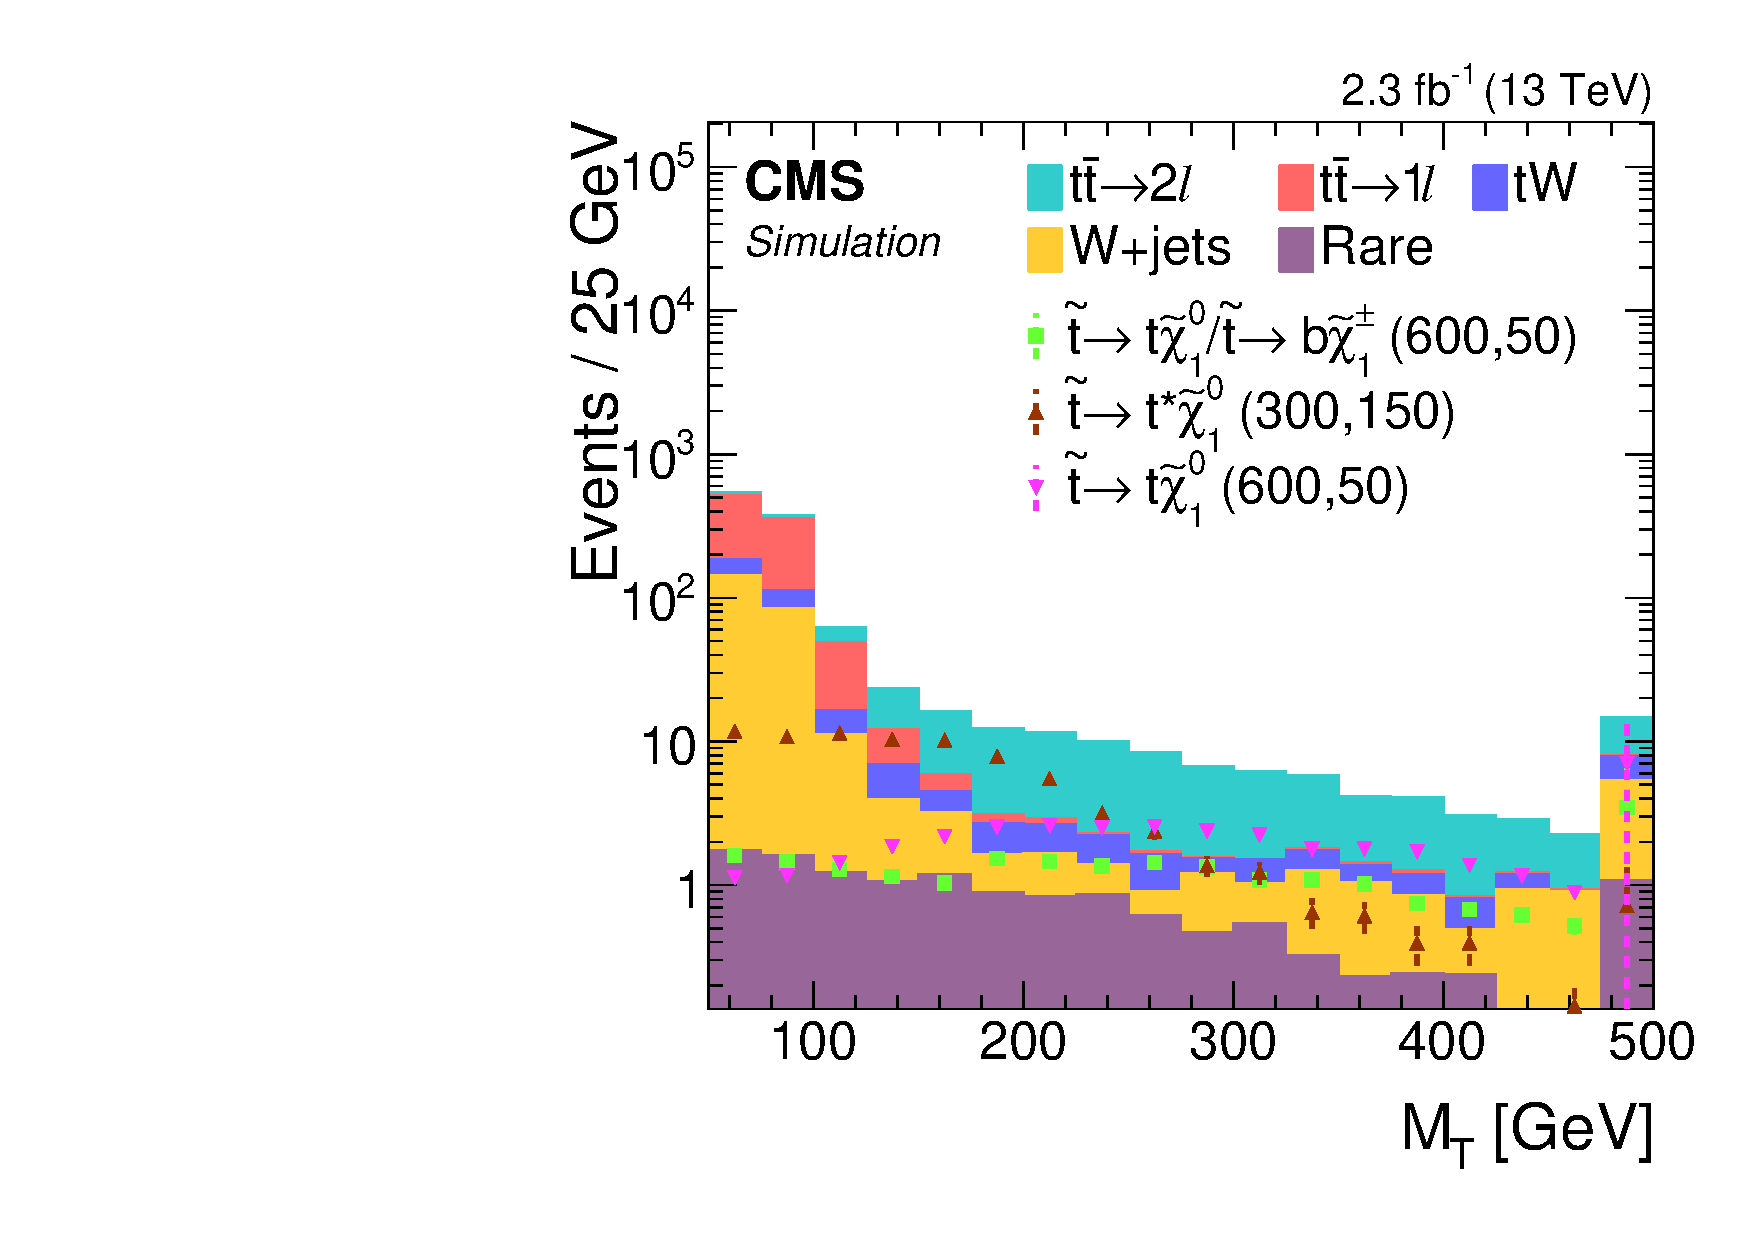
\includegraphics[width=0.6\textwidth]{figures/nminusone_mt.pdf}
\caption{Distribution of $\mt$ after all other selections have been applied.}
\label{fig:stop:mt:nminusone}
\end{figure}

\subsection{Modified Topness (\texorpdfstring{$\tmod$}{tmod})}
\label{ssec:stop:tmod}

In a previous search for stop squarks, particle physicists developed a
variable they called \emph{topness}, denoted $t$. This complicated
variable attempts to quantify the degree to which an event is
consistent with being a $\ttdilep$ event \cite{topness}. Although our
analysis must also suppress the $\ttdilep$ background, our
investigations showed that we could achieve better discrimination
between signal and $\ttdilep$ by removing two of the terms in the
topness variable (specifically, the center-of-mass constraint, and the
$\chi^2$ for leptonic top decay). We thus arrive at a variable we call
\emph{modified topness}, or $\tmod$. To calculate this
variable, we must minimize an expression that constrains the
neutrino-lepton system to have a mass similar to the W-boson mass, and the
b-quark-W-boson system to have a mass similar to top quark mass. Thus
we define:
\begin{equation}
\label{eq:stop:tmod}
\begin{split}
\tmod & = \ln ( \text{min} \; S ), \; \text{where} \\
S(\vec{p}_W, p_{\nu,z}) & = \frac{(m_W^2-(p_\nu+p_\ell)^2)^2}{a_W^4} + \frac{(m_t^2 - (p_{b_2}+p_W)^2)^2}{a_t^4}
\end{split}
\end{equation}

The parameters $a_W$ and $a_t$ provide the scale for the W-boson
and top quark masses; we set them to 5 GeV and 15 GeV, respectively.
There is some ambiguity as to which jets should be used in this
calculation. We found that $\tmod$ behaved best across signal
models with both low and high mass splittings if we chose our jets
according to these rules:
\begin{itemize}
\item Consider all combinations of the three jets with the highest
  CSVv2 discriminator values. If at least one such jet is b-tagged,
  only consider permutations that include at least one b-tagged jet.
\item Choose the combination of jets that minimizes the ultimate
  $\tmod$ value.
\end{itemize}
Ultimately, modified topness is effective in discriminating against
both $\ttdilep$ events and single top $tW$ events. However, it also
suppresses signal models with certain kinematics. For that reason, we
choose to bin our signal regions in $\tmod$, instead of making
a strict cut on it. Figure \ref{fig:stop:tmod} shows the distribution
of $\tmod$ for our background processes and various signal mass
points.

% Plot of t_mod adapted from AN-16-463.
\begin{figure}
\centering
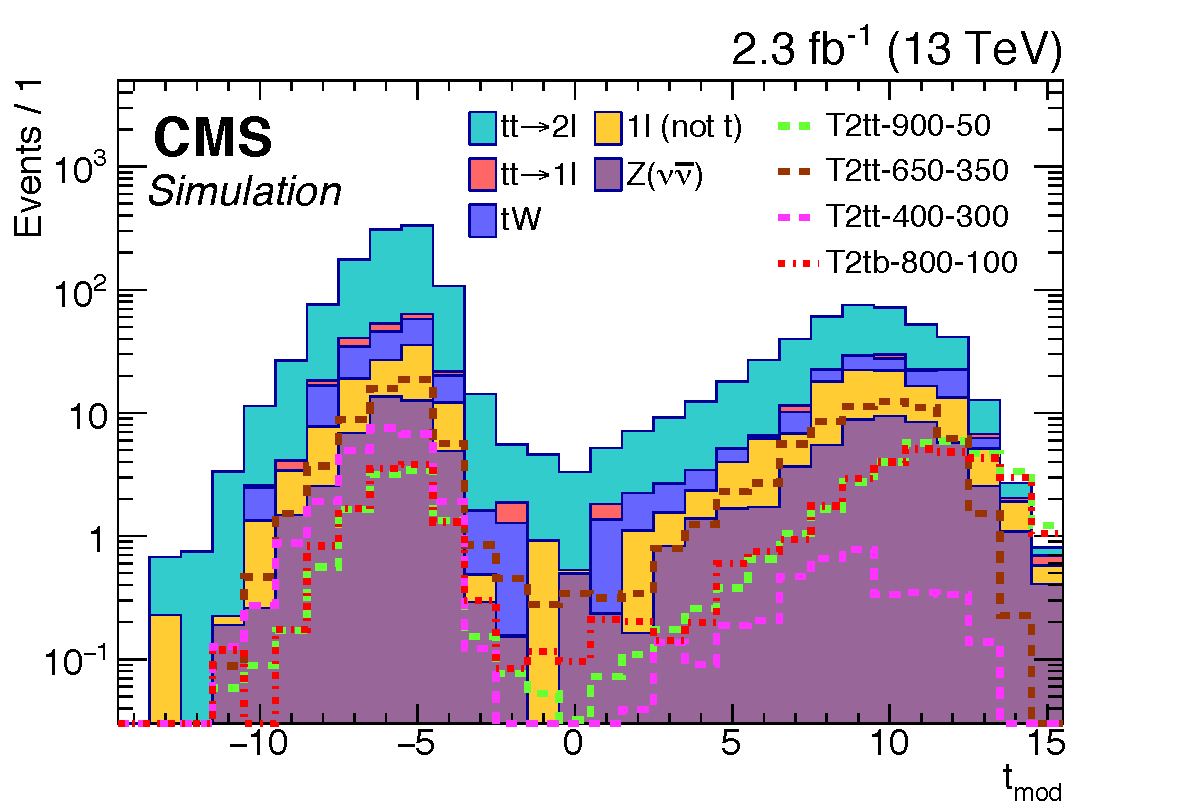
\includegraphics[width=0.6\textwidth]{figures/nminusone_tmod.pdf}
\caption{Distribution of $\tmod$ after all other selections
  have been applied. Normalization is arbitrary.}
\label{fig:stop:tmod}
\end{figure}

\subsection{Lepton-b Invariant Mass (\texorpdfstring{$\mlb$}{mlb})}
\label{ssec:stop:mlb}

Another variable that can help us discriminate signal from background
is the invariant mass of the lepton and its corresponding b-jet,
denoted $\mlb$. In the case of $\ttdilep$ and $\ttonelep$
backgrounds, as well as T2tt signals, assuming we pair our lepton with
the correct b-jet, then $\mlb$ is constrained by kinematics:
\begin{equation}
\mlb \leq \sqrt{m_t^2 - m_W^2} \approx 153 \text{GeV} % Verify this calculation for yourself!
\end{equation}
This inequality does not hold true for the W+jets background, nor for T2bW
signals. So a low-$\mlb$ requirement will reduce W+jets content
compared to the T2tt signal, and a high-$\mlb$ requirement will reduce
the $\ttbar$ backgrounds compared to the T2bW signal. As Section
\ref{sec:stop:sigregs} will describe, we use different bins of
$\mlb$ in the definitions of some of our signal regions.

We define $\mlb$ to be the invariant mass of the system of the
leading lepton and the b-tag nearest the lepton in $\Delta R$. Figure
\ref{fig:stop:mlb} shows an example distribution of this
variable. Because the W+jets background is dominant at higher
$\mlb$, and because W+jets has a much higher prevalence of
light-flavor jets over b-jets, we also tighten our b-tagging WP at
high $\mlb$.

% Mlb plot adapted from AN-16-463.
\begin{figure}
\centering
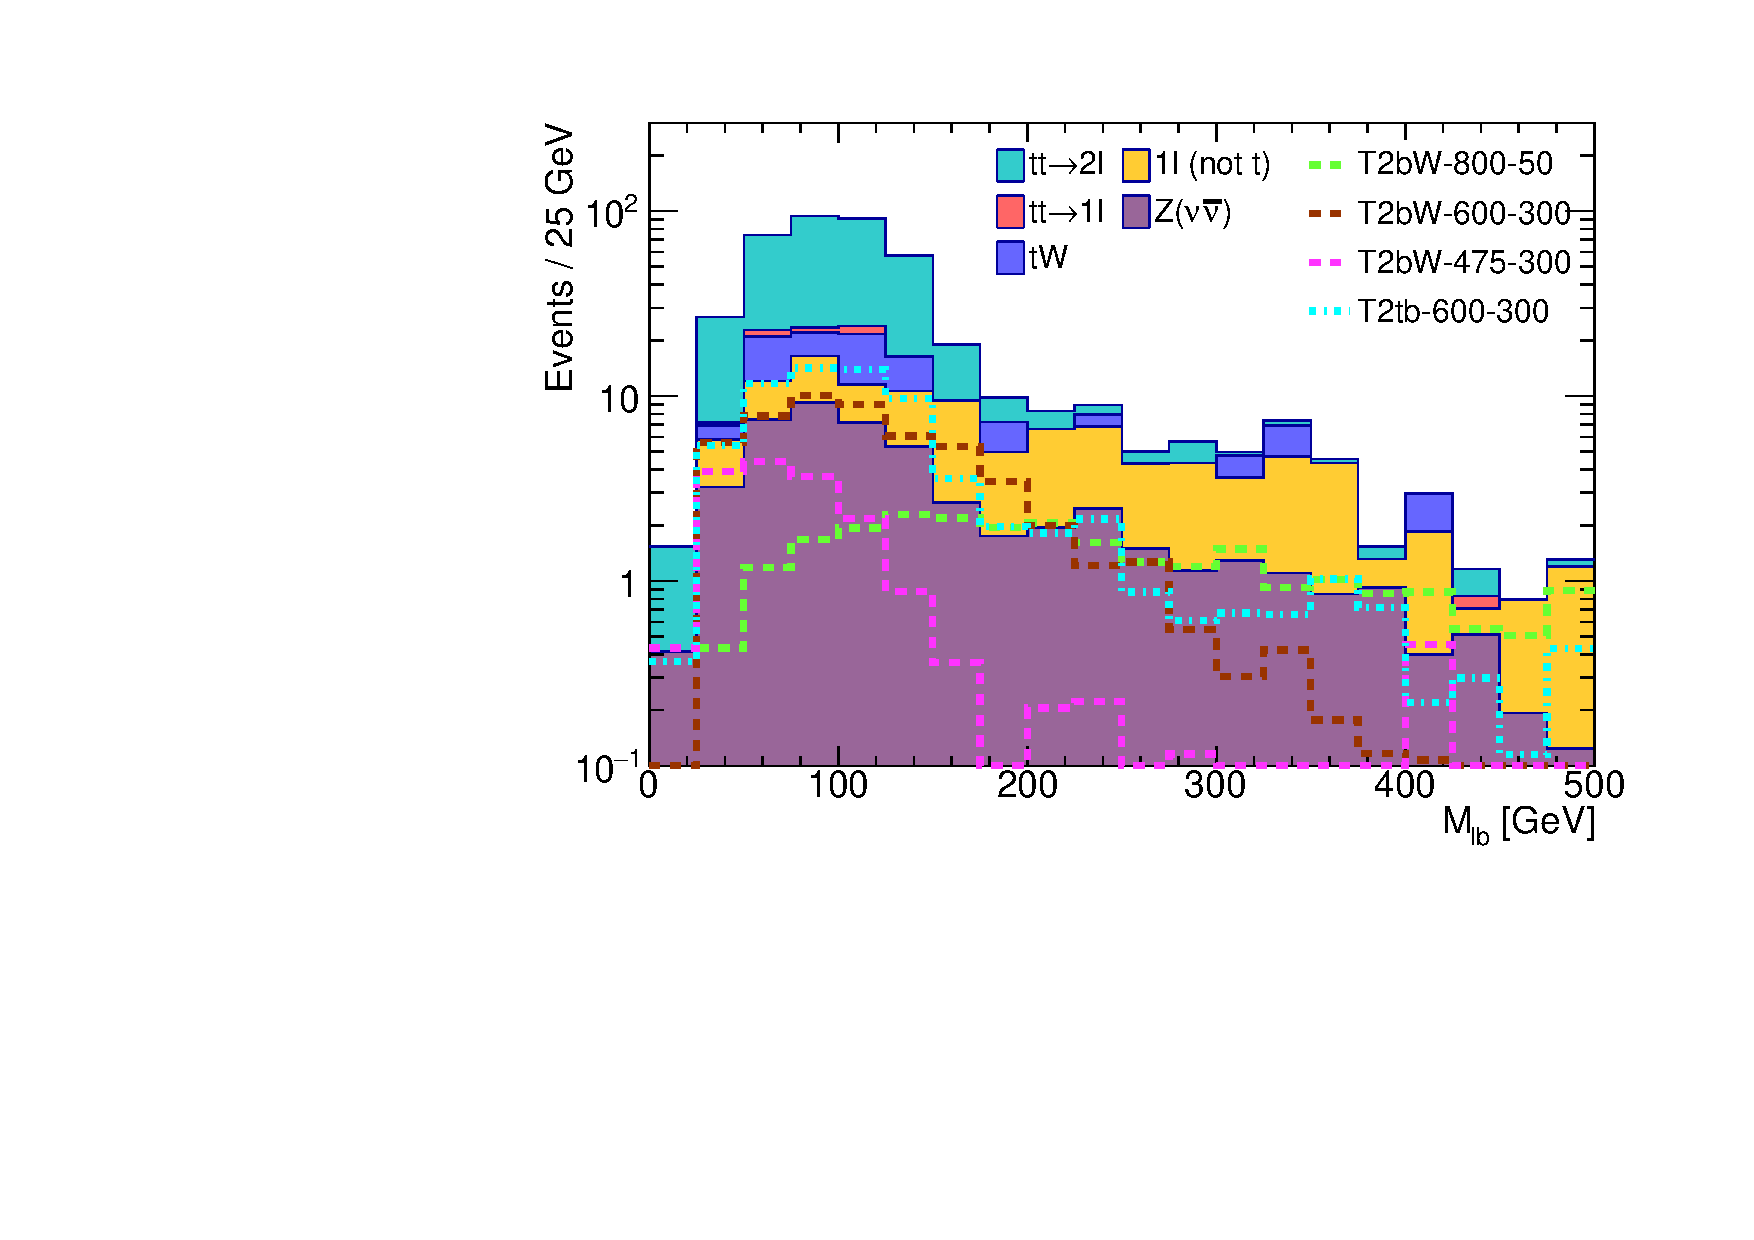
\includegraphics[width=0.6\textwidth]{figures/nminusone_mlb.pdf}
\caption{Distribution of $\mlb$ variable after baseline
  selections, in the region $\tmod > 0$. Normalization is arbitrary.}
\label{fig:stop:mlb}
\end{figure}

\subsection{Minimum Delta-Phi (\texorpdfstring{$\text{min}\Delta\phi(j_{1,2},\metvec)$}{minDphi})}
\label{ssec:stop:mindphi}

The final variable we consider in selecting our events is the minimum
$\Delta\phi$ between the $\metvec$ and either of the two leading
jets. In other words:
\begin{equation}
\text{min} \Delta\phi (j_{1,2},\metvec) = \text{min} \left\{ \Delta\phi
    (\metvec, j_1),\; \Delta\phi (\metvec, j_2) \right\}
\end{equation}
This variable allows us to reduce backgrounds such as $\ttdilep$ and
$\ttonelep$  with relatively little loss of signal, because in these
backgrounds we expect the neutrino (i.e. the source of the $\met$) to
be relatively close to the high-$p_T$ quark produced in the top
decay. Figure \ref{fig:stop:mindphi} shows the distribution of this
variable. We require a min$\Delta\phi >$ 0.8 for our bulk signal
regions; for the compressed T2tt search, this requirement is relaxed
to min$\Delta\phi >$ 0.5.

% Plot of MinDPhi taken from AN-16-463.
\begin{figure}
\centering
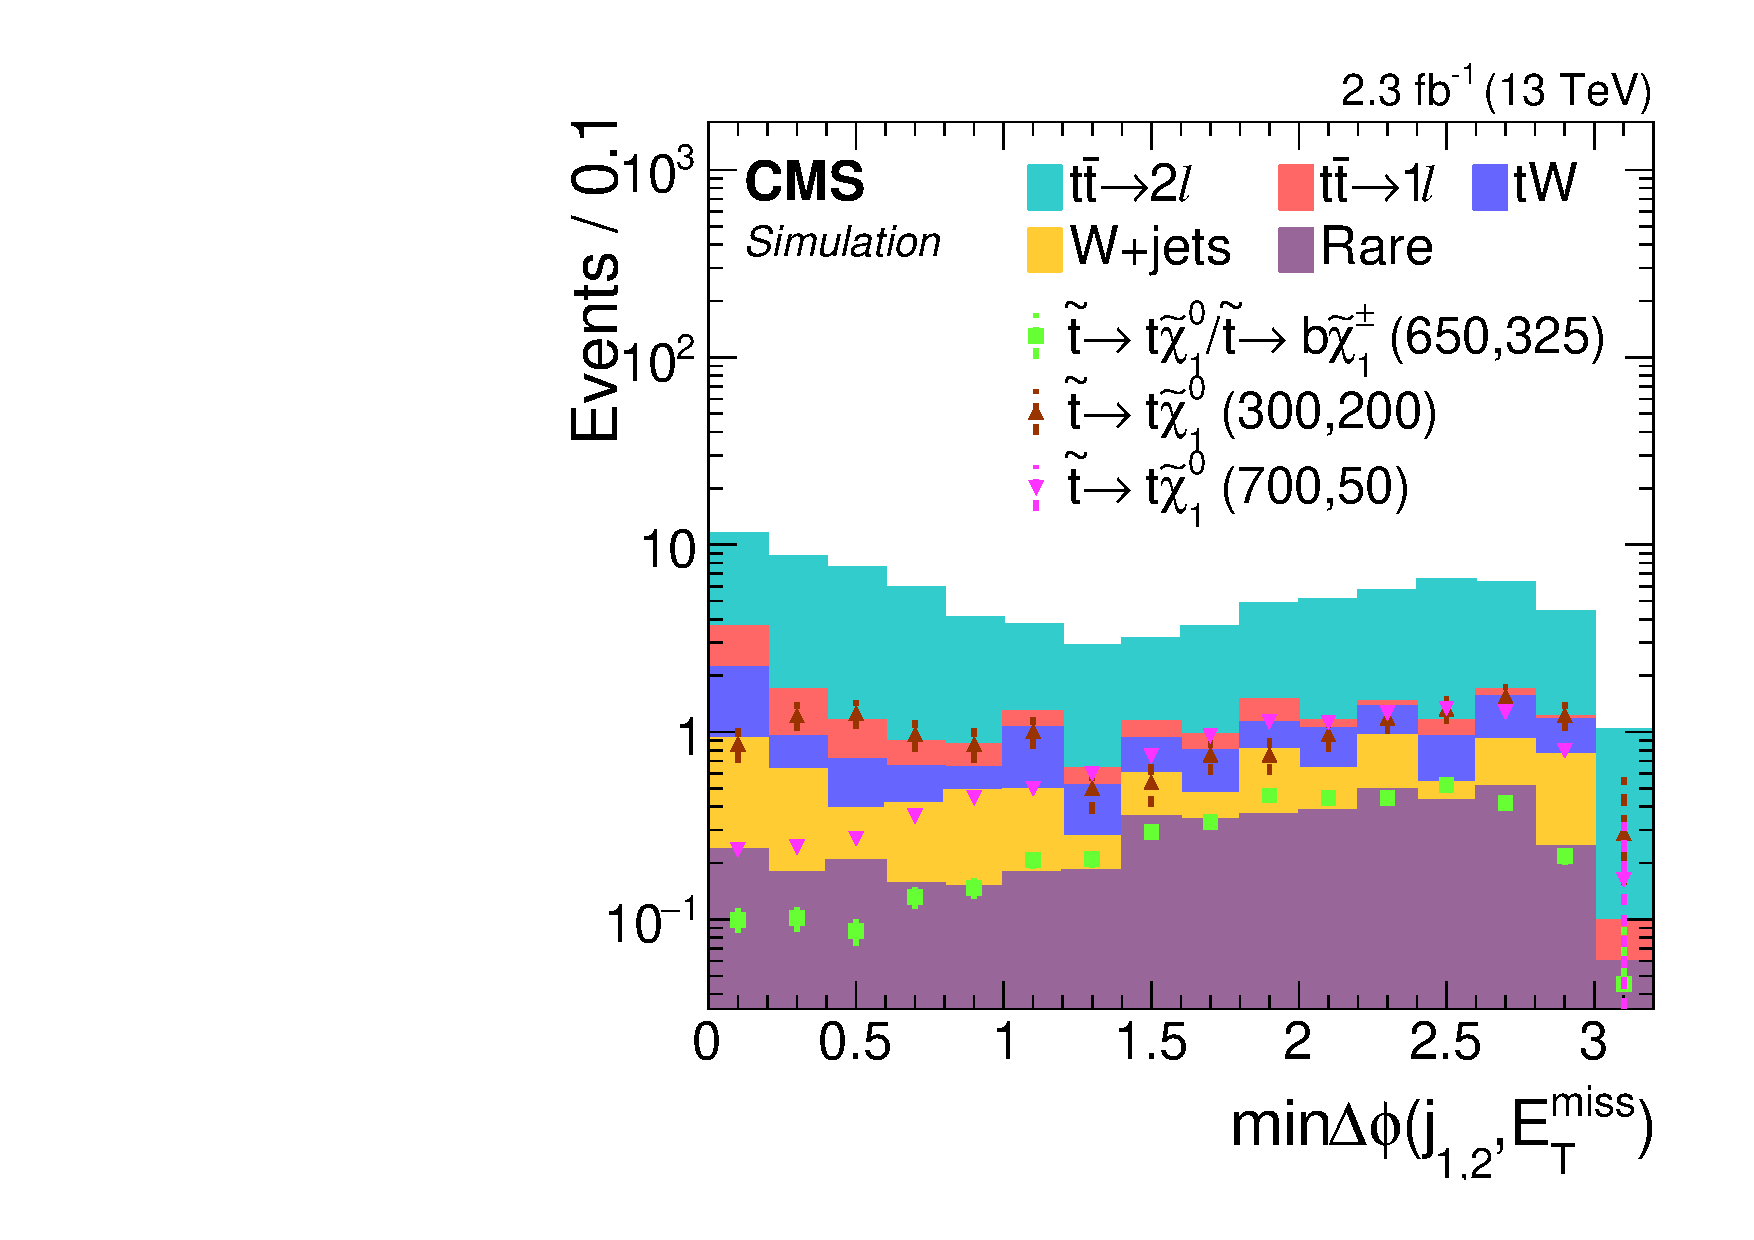
\includegraphics[width=0.6\textwidth]{figures/nminusone_mindphi.pdf}
\caption{Distribution of min$\Delta\phi (j_{1,2}, \metvec)$ after all
  other selections have been applied.}
\label{fig:stop:mindphi}
\end{figure}

\subsection{Corrections}
\label{ssec:stop:corrections}

Our Monte Carlo simulations seldom reproduce the aggregate properties of
real data with perfect accuracy. Therefore, we must reweight our
simulated events to reproduce the properties of the data more
exactly. The nominal weights applied to our MC simulations are
described here. Sections \ref{sec:stop:bkgest} and
\ref{sssec:stop:signal:systematics} will describe the systematic uncertainties
on these and other weights, and how we propagate those uncertainties
to our final results.

\begin{itemize}
\item As was described in Section \ref{ssec:stop:trigeff}, we evaluate
  the efficiencies of all triggers used in this analysis. For our
  signal regions, the combined trigger efficiency is so near 100\% that we
  do not reweight our MC; in the regions where we use dilepton
  triggers, we do apply a weight for the efficiency of those triggers.
\item We apply the official jet energy corrections from CMS, as mentioned in
  Sections \ref{ssec:stop:jets} and \ref{ssec:stop:met}.
\item We apply weights to mimic the efficiency of our b-tagging
  algorithms. These weights are provided by the b-tagging POG within
  CMS. There are separate weights for heavy flavor (HF) and light
  flavor (LF) jets, as well as for the medium and tight WPs used in
  the analysis.
\item We apply weights for the efficiency of lepton identification and
  isolation, as provided by the SUSY group in CMS. We also account for
  the efficiency of vetoing a second lepton where applicable. Separate
  weights must be applied to our signal samples because they were
  generated using FastSim.
\item Initial state radiation (ISR) refers to partons (and the jets
  they produce) that radiate off the
  incoming particles in the hard collision process. ISR is not
  necessarily modeled correctly in our Monte Carlo samples. We
  reweight our simulated events using a prescription from the SUSY
  group to obtain a more accurate distribution of the number of jets
  per event.
\item All of our signal and control regions involve binning in
  $\met$. If the $\met$ resolution differs between data and MC, we run
  the risk of badly estimating how simulated events are distributed
  among these bins. In Appendix
  \ref{apx:stop:metres}, we perform a separate study on the effects
  of $\met$ resolution mismodeling, and the results are used to
  reweight our $\ttbar$, single top $tW$, and W+jets simulated events.
\item As Appendix \ref{apx:stop:emustudies} describes, there is a disagreement
  between data and MC in the tail of the $\met$ spectra of dileptonic
  $\ttbar$ and $tW$ events. Thus, we correct this discrepancy by
  applying a weight to dileptonic $\ttbar$ and $tW$ MC
  events in the upper $\met$ range where this effect would impact our measurements.
\item To correct for discrepancies in the pileup distribution, we
  reweight events using the official corrections prescribed by CMS.
\end{itemize}

\section{Signal Regions}
\label{sec:stop:sigregs}

As Section \ref{sec:stop:selections} has described, we preselect events
for our search using the following criteria:
\begin{itemize}
\item The first vertex must meet certain quality criteria.
\item The event must have one well-reconstructed electron or
  muon. There must be no other electrons or muons in the event, even
  of low reconstruction quality.
\item The event must not have a tau in it, or an isolated track that
  could be a tau.
\item The event must have at least two jets, of which at least one
  must be b-tagged.
\item The $\met$ must be at least 250 GeV.
\item The $\mt$ must be at least 150 GeV.
\item The minimum $\Delta \phi$ between the $\met$ and the two leading
  jets must be at least 0.8; at least 0.5 for the corridor search.
\end{itemize}
After those criteria have been met, events are further subdivided
among several different signal regions, to increase our sensitivity to
a wide variety of SUSY scenarios.

\subsection{Nominal Signal Regions}
\label{ssec:stop:sigregsnominal}

Our nominal signal regions are tailored to the search for most T2tt
signals, the T2bW signals, and the T2tb signals. To that end, our
signal regions are divided by the number of jets in the event, the
modified topness variable, the lepton-b-jet invariant mass, and the
amount of $\met$. These signal regions are enumerated in Table
\ref{tab:stop:nominalsrs}. At times I will refer to these regions using a
letter for the series and a number for the specific $\met$ bin, as
A3, D1, G4, etc.

% Table of nominal SRs adapted from AN-16-463.
\begin{table}[htb]
\centering
\caption{Definitions of the signal regions used in the nominal search.}
\label{tab:stop:nominalsrs}
\begin{tabular}{|c|c|r|r|lllll|}
\hline
Label & $N_J$ & $\tmod$ & $\mlb$ [GeV] & \multicolumn{5}{c|}{$\met$ [GeV]} \\
\hline
A & 2-3     & $>10$ & $\leq175$     & 250-350 & 350-450 & 450-600 & $>600$ & \\
B & 2-3     & $>10$ & $>175$        & 250-450 & 450-600 & $>600$ & & \\
C & $\geq4$ & $\leq0$ & $\leq175$   & 250-350 & 350-450 & 450-550 & 550-650 & $>650$ \\
D & $\geq4$ & $\leq0$ & $>175$      & 250-350 & 350-450 & 450-550 & $>550$ & \\
E & $\geq4$ & 0-10 & $\leq175$      & 250-350 & 350-550 & $>550$ & & \\
F & $\geq4$ & 0-10 & $>175$         & 250-450 & $>450$ & & & \\
G & $\geq4$ & $>10$ & $\leq175$     & 250-350 & 350-450 & 450-600 & $>600$ & \\
H & $\geq4$ & $>10$ & $>175$        & 250-450 & $>450$ & & & \\
\hline
\end{tabular}
\end{table}

The signal regions that require 2-3 jets and $\tmod >$ 10
(the A and B series) are
designed to target T2tb signals. Because we take the mass difference
between the chargino and the LSP to be only 5 GeV in this model, the
W-boson produced in the chargino to LSP decay will be very off
shell. Thus the lepton will come from the top decay, and the off-shell
W will decay into very weak jets that we cannot resolve. In addition,
these regions will also have sensitivity to any of our signal models
where the stops are highly boosted and cause two jets to merge into one.

The remaining nominal signal regions (C-H) target T2tt and T2bW
models. They include a four jet requirement because we expect two b-jets from the
top or stop decays and two more jets from the hadronic W decay.

Each of our three signal models peaks in a different part of the
$\tmod$ range. So by creating three distinct bins in
$\tmod$ (but not applying a cut), we can target each model in
a different region, while effectively dividing the background events into three
parts. As Figure \ref{fig:stop:tmod} shows, the compressed
case (small $\Delta M$) is most prominent when
$\tmod$ is $<$ 0. When $0 < \tmod < 10$, signal models
with moderate $\Delta M$ will stand out most against
$\ttdilep$. And when $\tmod >$ 10, the $\ttdilep$ background
drops off substantially faster than signals with a large $\Delta M$.

The binning in $\mlb$ follows from the facts explained in
Section \ref{ssec:stop:mlb}. At low $\mlb$, the W+jets
background is reduced with little loss in the T2tt signal, and at high
$\mlb$, the $\ttbar$ backgrounds are reduced for little loss in
the T2bW signal. Because this reduction in $\ttbar$ leaves W+jets as
the dominant background, we also require that our one b-tag pass a
tight WP in the in the high $\mlb$ regions.

Finally, the higher the mass splitting, the more $\met$ we generally
expect in an event. So binning in $\met$ increases the
likelihood that any one particular signal model will stand out against the
SM background. We choose how many $\met$ bins to use in each series,
and where their boundaries should be, in order to give reasonable
statistics in all signal regions.

\subsection{Corridor Signal Regions}
\label{ssec:stop:sigregscorridor}

As Section \ref{ssec:stop:sigcompressed} described, previous stop
searches have struggled to achieve sensitivity in the top corridor
region because compressed T2tt decays are suppressed and difficult to
detect. In order to address this deficit, I developed a dedicated
search strategy focused on increasing our acceptance of compressed
T2tt signals, while maintaining a low rate of SM background
events. I also validated that this strategy was compatible with our
established techniques for background and signal estimation. The final
product of my work was four additional signal
regions to add to our overall search strategy.

The dedicated corridor signal regions use the same event selections as
the nominal signal regions, except for the following changes:
\begin{itemize}
\item I require at least 5 jets in the event.
\item The highest-$p_T$ jet must not be b-tagged using the medium WP.
\item The $p_T$ of the lepton in the event must be $<$ 150 GeV.
\item The azimuthal angle between the $\met$ and the lepton, $\Delta
  \phi (\met, \ell)$, must be $<$ 2.0.
\item As described earlier, the min$\Delta \phi(j_{1,2},\metvec)$
  must be $>$ 0.5.
\end{itemize}
In addition to these selections, the four corridor signal regions are
defined by four bins in $\met$, given by Table \ref{tab:stop:corridorsrs}:

% Table of corridor SR met bins, adapted from AN-16-463.
\begin{table}[h]
\centering
\caption{$\met$ bins used in the dedicated corridor signal regions.}
\label{tab:stop:corridorsrs}
\begin{tabular}{|c|cccc|}
\hline
Label & \multicolumn{4}{c|}{$\met$ [GeV]} \\
\hline
I & 250-350 & 350-450 & 450-550 & $>550$ \\
\hline
\end{tabular}
\end{table}

To develop these signal regions, I considered the unique kinematics of
compressed T2tt signals, and how they might affect the variables
already employed in our stop search. I also considered whether any new
variables might be able to discriminate compressed T2tt from the SM
background. Although several variables had the potential to
discriminate compressed T2tt from background, I made the final choice
by measuring which added cuts provided the greatest increases in
expected sensitivity, measured using a simplified version of the
limit-setting procedure described later in Section
\ref{sec:stop:interp}.

Compressed stop decays, by virtue of their off-shell top quark, tend
to have lower $\met$ than the bulk signals. So one of the first
modifications I considered was relaxing our $\met$
requirement. However, I found that any reduction in $\met$ would cause a
proportionally larger increase in background yield than in signal
yield. With the 250 GeV $\met$ cut firmly fixed in place, we then
asked how might a compressed stop decay generate such large $\met$?
The answer to that question ultimately became the defining element of
the corridor search strategy.

We concluded that in the corridor region, in order to generate at least
250 GeV of $\met$, a stop pair must have a large boost. Momentum conservation
dictates that in order to have a large boost, the stop pair should be
recoiling off some other physics object. The most likely candidate was
a high-$p_T$ jet produced as ISR. Because we expected another jet in
the event, in addition to the four from stop decay, we imposed the
$N_J > 5$ requirement. Additionally, ISR jets seldom originate from
b-quarks, because b-quarks are fairly heavy, and thus hard to
produce. So we further target the compressed signal by requiring
that the leading jet not be b-tagged.

% N-1 plots, made by moi, but sourced from AN-16-463.
\begin{figure}[htb]
\centering
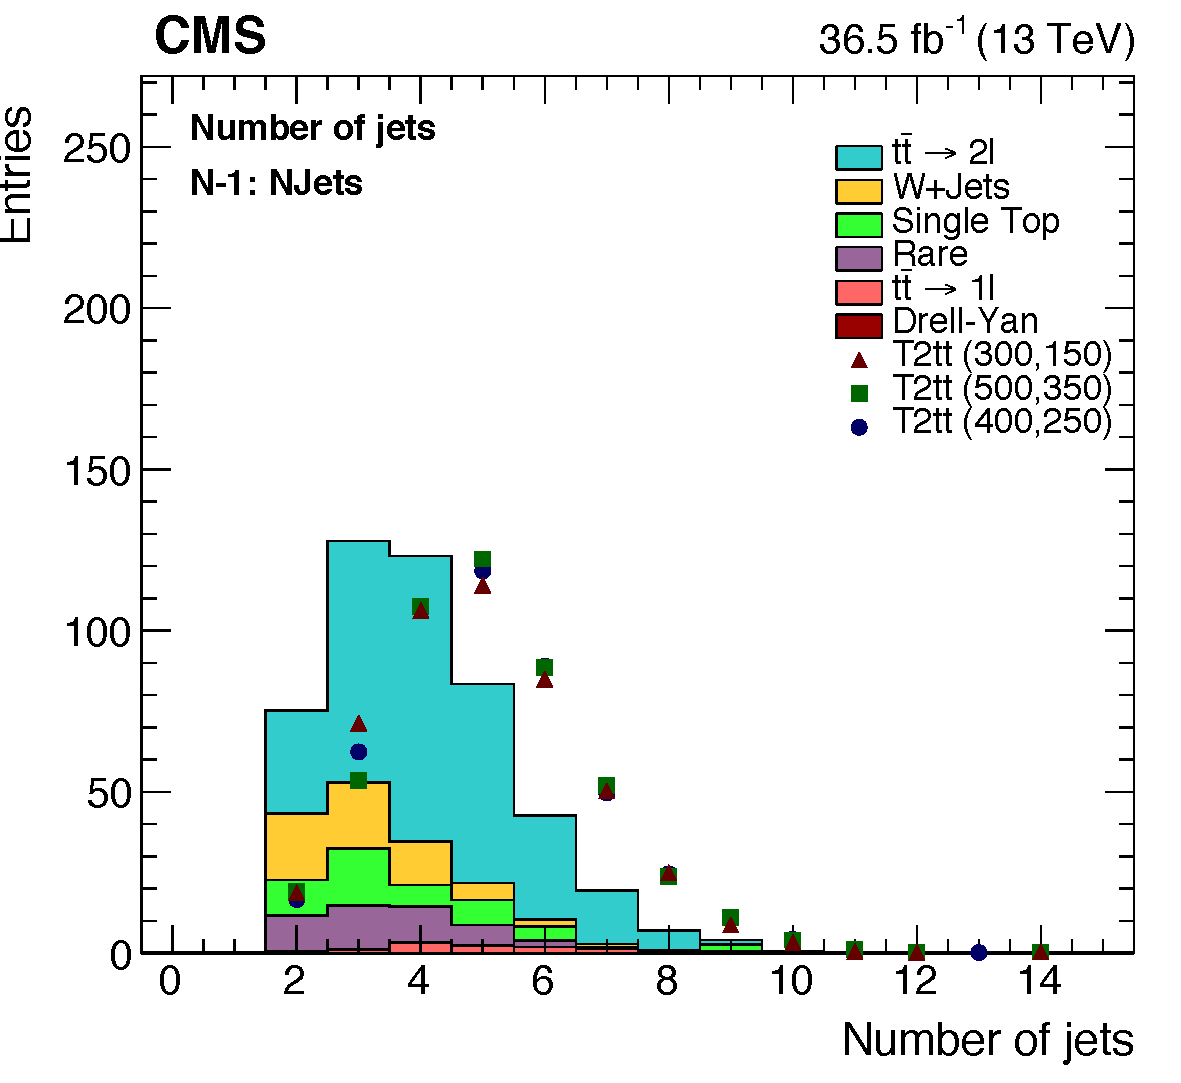
\includegraphics[width=0.45\textwidth]{figures/nminus1_njets.pdf}
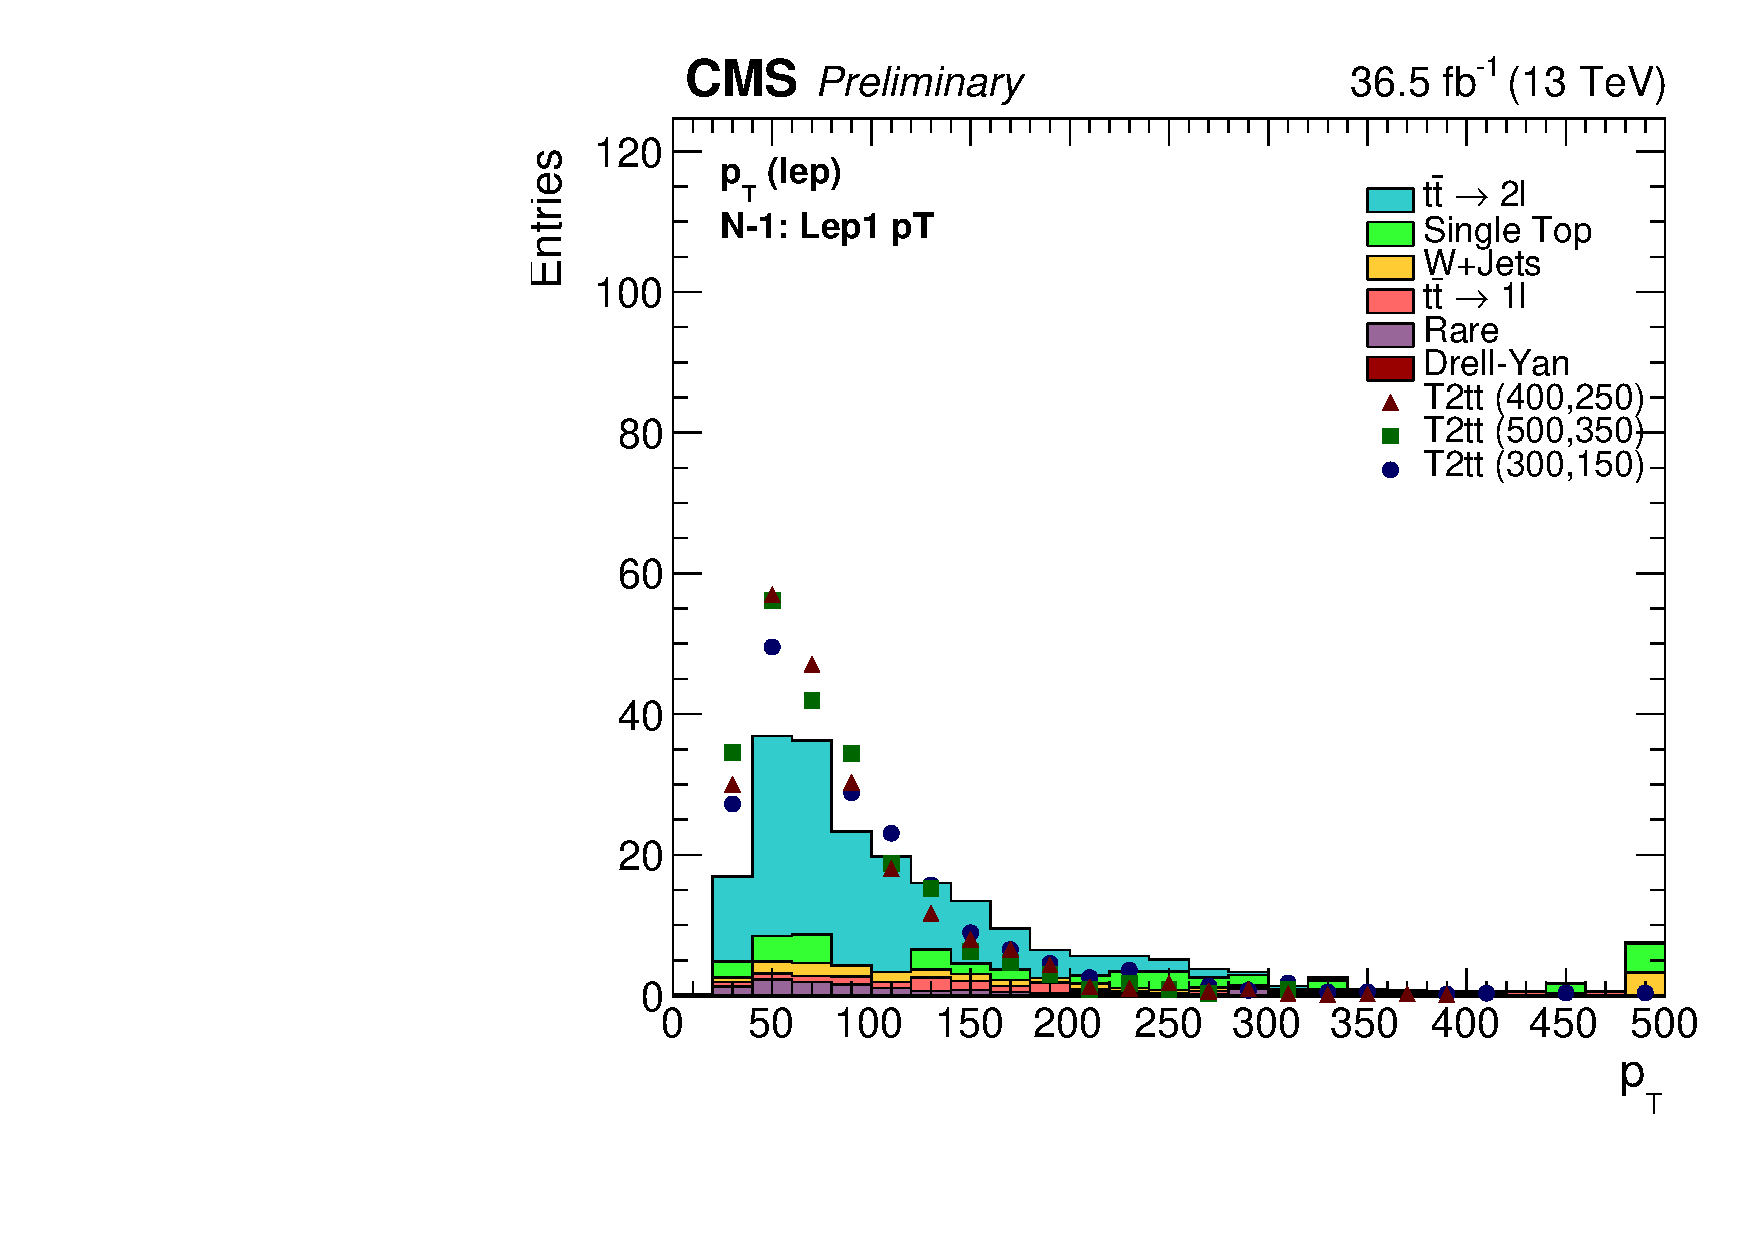
\includegraphics[width=0.45\textwidth]{figures/nminus1_ptlep.pdf}
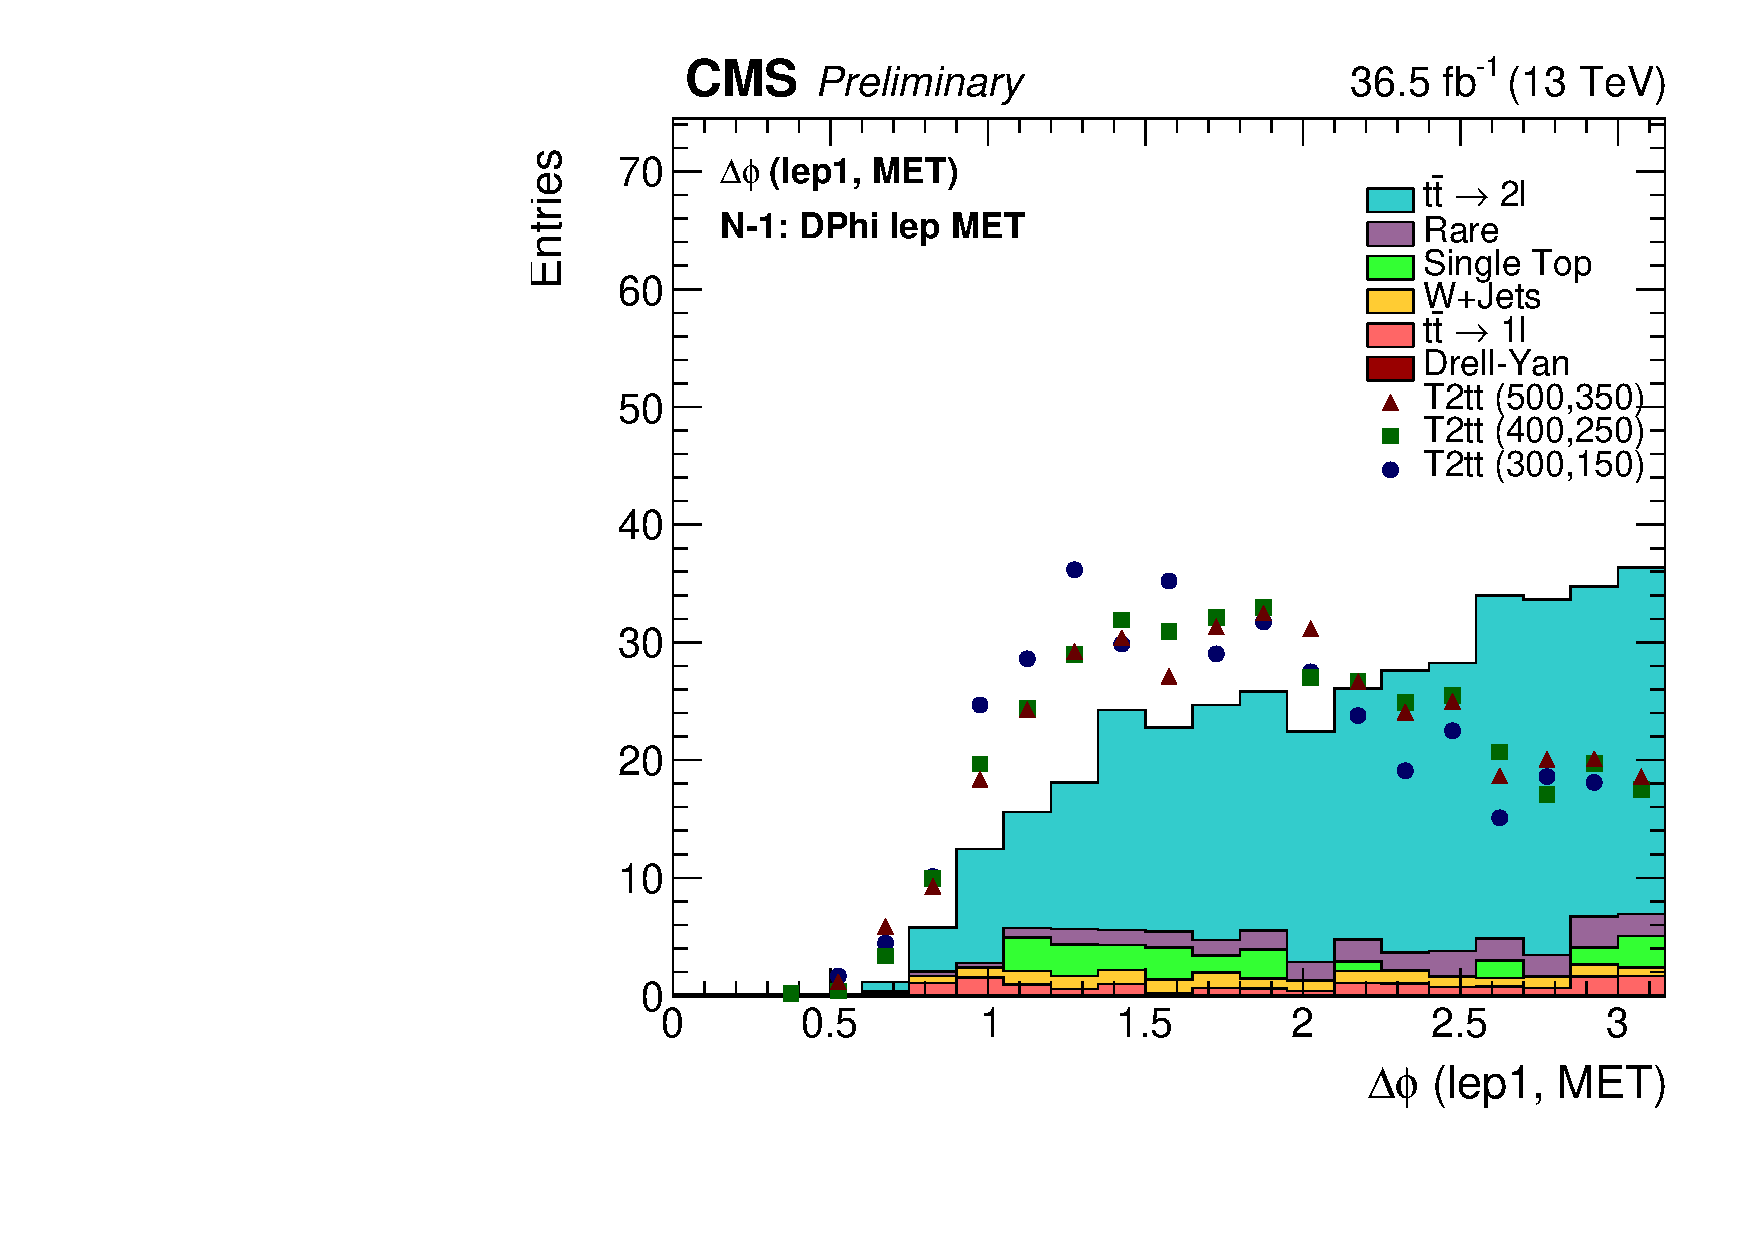
\includegraphics[width=0.45\textwidth]{figures/nminus1_dphilmet.pdf}
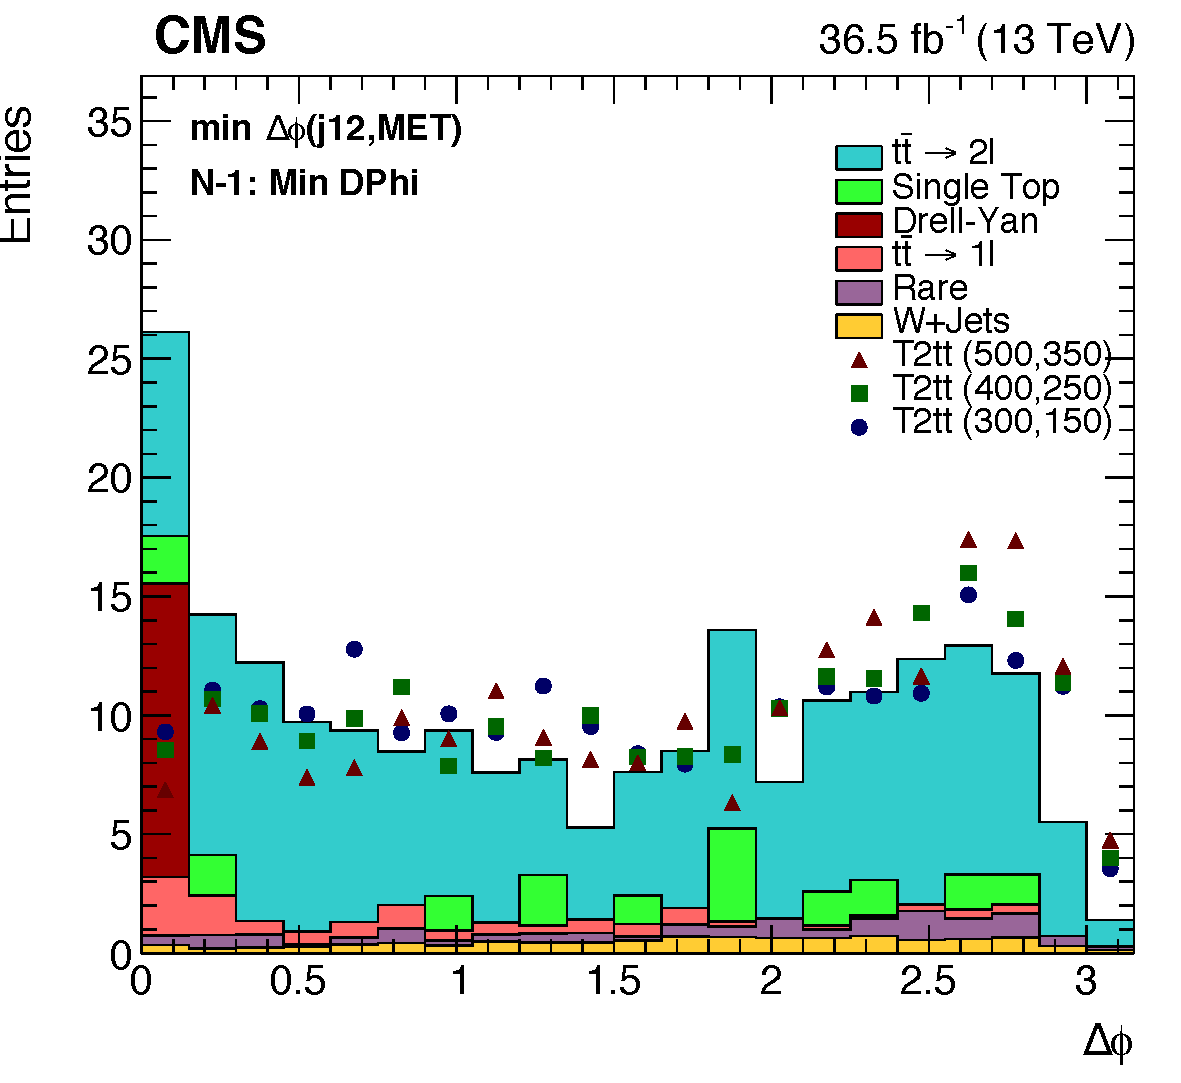
\includegraphics[width=0.45\textwidth]{figures/nminus1_mindphi.pdf}
\caption{Comparison between background and selected signal points for
  the four (non-boolean) variables that define the corridor signal
  regions. Each cut is removed, to illustrate the rationale for its
  threshold.}
\label{fig:stop:corridor:nminusone}
\end{figure}

The $\met$ in a stop decay comes from the two LSPs, as well as the
neutrino produced alongside the single lepton. In the case where the
stop squarks are boosted, we expect the products of the stop decays,
including the main contributors to the
$\met$, to continue in the rough direction of their parents too. Thus the cut
$\Delta\phi (\met, \ell) < 2$ selects events where the lepton and the
$\met$ are not separated by a large angle. Similarly, by relaxing
the cut on min$\Delta \phi(j_{1,2},\metvec)$ to $>$ 0.5, we allow jets
produced in the stop decays to be more colinear with the lepton.
Finally, the upper bound on the lepton $p_T$ is because compressed top
quarks have less momentum to pass on to their decay products.
The distributions of these variables are pictured in Figure
\ref{fig:stop:corridor:nminusone}.

It is worth noting that the dedicated corridor signal regions are not
orthogonal to the nominal signal regions. In fact, if not for the
relaxed min$\Delta\phi$ cut, the corridor signal regions would
constitute a strict subset of the nominal signal regions. To avoid
double-counting events in multiple signal regions, we decided to use
the corridor and nominal signal regions in non-overlapping regions of
parameter space. Using the statistical tools described in Section
\ref{ssec:stop:limits}, I calculated the expected sensitivity to T2tt
signals for both the nominal and corridor signal regions at a variety
of mass points. The sensitivity is expressed as a number, $r$, the
smallest value by which one could scale the signal cross section and
be able to exclude the signal hypothesis. Put simply, lower values
of $r$ indicate greater sensitivity to the signal. In Figure
\ref{fig:stop:rratio}, I plotted the ratio
$r_\text{corridor} / r_\text{nominal}$ for T2tt signals; wherever that value is less
than 1, the corridor signal regions are expected to be more sensitive
than the nominal signal regions. Perhaps unsurprisingly, the corridor search
regions have higher expected sensitivity for $\Delta M$ between 100 and
225 GeV--in other words, in the area around and between the top and W
corridors. The size of the improvement in sensitivity ranges from
about 10-30\%. We therefore use only the corridor signal regions for
T2tt models with $\Delta M$ between 100 and 225 GeV, and we use only
the nominal signal regions elsewhere in the T2tt plane, and for the
T2bW and T2tb signal models.

% r-ratio between corridor and nominal signal regions. Originally made
% by moi, then taken from AN-16-463, then further tweaked.
\begin{sidewaysfigure}
\centering
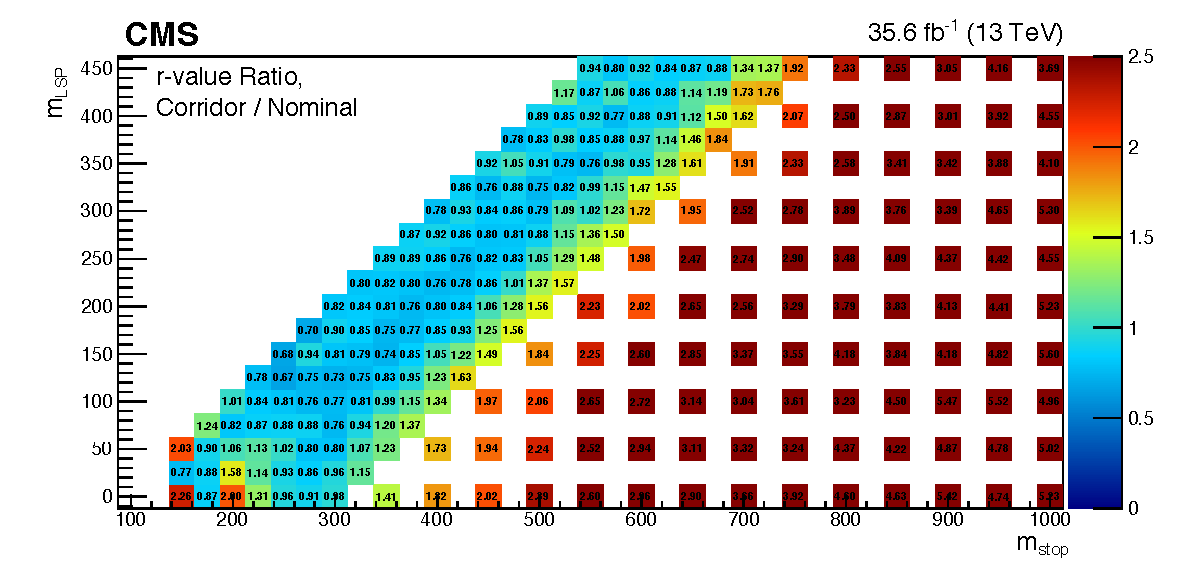
\includegraphics{figures/rratioplot.pdf}
\caption{Ratio of expected sensitivities for the corridor and nominal
  signal regions, at every mass point in the T2tt signal scan.}
\label{fig:stop:rratio}
\end{sidewaysfigure}


\section{Background Estimation}
\label{sec:stop:bkgest}

As previous sections have described, we apply a number of
preselections that reduce the prevalence of the SM backgrounds in our
search. In addition, we divide our search up into signal
regions so that we can hunt for several possible signal models while
spreading out the backgrounds. However, even with these measures,
we still expect our signal regions to be dominated by SM background
events. If we hope to find any signal from SUSY among the backgrounds,
we must be able to reliably estimate the size of the backgrounds so we
can subtract them from the measured data. We make these estimates
using a variety of techniques that will be described below. Wherever
possible, we make data-driven estimates by looking at control regions
(CRs) that are adjacent or complementary to our signal regions. In
general, the same strategies are applied to estimate backgrounds for
both the nominal and corridor signal regions. This section will also
describe how we estimate the systematic uncertainties on each
background component.

\subsection{Lost Lepton}
\label{ssec:stop:lostlep}

Across all our signal regions, the largest total background
is the lost lepton background. These are events that have two true
leptons in them, but for various reasons, the second lepton is not
caught by our second lepton veto, hadronic tau veto, or isolated track
veto. Often this loss occurs because the additional lepton is poorly
reconstructed, or falls outside the $|\eta|$ or $p_T$ ranges we can
detect. Because the second lepton is not detected, it effectively
creates additional $\met$, helping the event to pass our $\met$
requirement. Plus the additional neutrino associated with the second
lepton can help the event pass our $\mt$ cut. The dominant physics
process contributing to this background is $\ttdilep$, however there
is a strong contribution from single-top production in the $tW$
channel. Other contributors include $\ttbar$ + vector boson
production, and diboson production. The strong understanding of the
$\ttdilep$ process gained in the top asymmetry measurements (Chapter
\ref{chap:afb}) gives us confidence we can accurately estimate this
background component.

\subsubsection{Estimation Method}
\label{sssec:stop:lostlep:estimation}

We estimate the number of lost lepton events in our signal regions
based on the number of events in a set of dilepton control regions, to be
defined below. We assume that Monte Carlo simulations correctly model
the ratio of lost lepton events to dilepton events, so that the
following relationship holds true:
\begin{equation}
\label{eq:stop:lostlep:rationm}
\frac{N_{\text{lost }\ell}^\text{Data, SR}}{N_{\ell\ell}^\text{Data, CR}} =
\frac{M_{\text{lost }\ell}^\text{MC, SR}}{M_{\ell\ell}^\text{MC, CR}}
\end{equation}
In this and future equations, $N$ will denote the number of events in
actual data, and $M$ will denote the number of events in Monte Carlo
simulations.

By rearranging Equation \ref{eq:stop:lostlep:rationm}, we can derive
a data-driven estimate for the number of lost lepton events in the
signal region, using the data yield in the corresponding control region
times the SR/CR ratio derived from Monte Carlo. This ratio is known as
the lepton transfer factor, $TF_\text{lep}$. So:
\begin{equation}
\label{eq:stop:lostlep:estimate}
N_{\ell\ell}^\text{SR} = N_{\ell\ell}^\text{CR} \times \frac{M_{\ell\ell}^\text{SR}}{M_{\ell\ell}^\text{CR}}
\end{equation}

Five of the high-$\met$ CRs have very small data yields, a fact that
would contribute to large statistical uncertainty using the
estimation method described above. To mitigate this uncertainty, we
combine the low-statistics bins with their neighboring bins that have
higher statistics, and add another term where we use MC to extrapolate
from the merged $\met$ bins to the single $\met$ bins:
\begin{equation}
\label{eq:stop:lostlep:metextrap}
N_{\ell\ell}^\text{SR, bin} = N_{\ell\ell}^\text{CR, merged} \times \frac{M_{\ell\ell}^\text{SR, merged}}{M_{\ell\ell}^\text{CR, merged}}
\times \left( \frac{M_{\ell\ell}^\text{SR, bin}}{M_{\ell\ell}^\text{SR, merged}} \right)
\end{equation}
The specific regions that are merged in this way are: B2/3, E2/3,
F1/2, and H1/2.

This process of extrapolating in $\met$ has the potential to introduce
errors in our measurements if the $\met$ distribution or $\met$ resolution
are mismodeled in MC. In Appendix \ref{apx:stop:emustudies}, we study
the modeling of dileptonic $\ttbar$ and $tW$ events using an $e/\mu$ cross-check
region, and in Appendix \ref{apx:stop:metres} we study the modeling of the
$\met$ resolution. Based on these studies, we assign appropriate scale
factors and systematic uncertainties to account for any effects due to
mismodeling. The $\met$ extrapolation also introduces some additional
uncertainty due to limited MC statistics.

\subsubsection{Control Region Definitions}
\label{sssec:stop:lostlep:crdefinitions}

To form our dilepton control regions, we use the same selections and
binning as the signal regions, except that we invert the veto on
additional leptons. Whereas the signal regions require the absence of
a second electron or muon, our dilepton control regions require the
presence of a second reconstructed electron or muon passing the
veto ID (described earlier), and with $p_T >$ 10 GeV. To simplify
our estimate and its uncertainties, we do not invert the
hadronic tau or isolated track vetos. Because lost leptons contribute
to $\met$ in our signal regions, when working with the dilepton
control regions we add the trailing lepton $p_T$ to the $\met$, and
recalculate all derived quantities that are based on $\met$. This
helps us keep the conditions as similar as possible between the CRs
and the SRs.

The data and MC yields in the dilepton control regions are given in
Table \ref{tab:stop:lostlep:cryields}. The events in the control
regions receive all the same corrections as the SR
events, with two exceptions. For dilepton events with a hadronic tau
in them, we apply a scale factor to correct the efficiency of tau
identification. We also apply different trigger weights, because we
select dilepton events using dilepton triggers.
Our control regions are over 95\% pure in dilepton events,
so we make no correction for impurities. The rightmost column of Table
\ref{tab:stop:lostlep:cryields} presents the ratio of the data to MC
yields. In some regions, this ratio differs considerably from
unity. Such differences in normalization between data and MC
actually have no effect on our final background estimate. Looking at Equation
\ref{eq:stop:lostlep:estimate}, we see that the background
normalization comes entirely from the CR data, and that MC is used
only to calculate the transfer factor from the CRs to SRs (and the
$\met$ extrapolation factor, where relevant).

% Dilepton CR yield table, adapted from AN-16-463.
\begin{sidewaystable}
\centering
{\scriptsize
\caption{Data and Monte Carlo yields in the dilepton control regions,
  based on 35.9 fb\textsuperscript{-1} of luminosity.}
\label{tab:stop:lostlep:cryields}
\begin{tabular}{|l|c c c c c|c|c|}
\hline
Region  & $\ge2$~leptons & $1$~lepton,~from~$W$ & $1$~lepton,~from~$t$ & $Z\rightarrow\nu\nu$ & Sum Bkg. & Data & Data/MC \\*
\hline \hline
$<4$ jets,~$\tmod \ge10$,~$\mlb<175$,~$250<\met<350$  & 215.40 $\pm$ 4.56  & 4.27 $\pm$ 2.62  & 6.49 $\pm$ 0.95  & 1.35 $\pm$ 0.06  & 227.51 $\pm$ 5.35  & 217 $\pm$ 14.73  & 0.95 $\pm$ 0.07 \\*
$<4$ jets,~$\tmod \ge10$,~$\mlb<175$,~$350<\met<450$  & 77.88 $\pm$ 2.80  & 0.27 $\pm$ 0.13  & 2.61 $\pm$ 0.62  & 0.65 $\pm$ 0.04  & 81.40 $\pm$ 2.87  & 75 $\pm$ 8.66  & 0.92 $\pm$ 0.11 \\*
$<4$ jets,~$\tmod \ge10$,~$\mlb<175$,~$450<\met<600$  & 25.01 $\pm$ 1.63  & 3.33 $\pm$ 3.08  & 1.37 $\pm$ 0.44  & 0.23 $\pm$ 0.03  & 29.95 $\pm$ 3.51  & 25 $\pm$ 5.00  & 0.83 $\pm$ 0.19 \\*
$<4$ jets,~$\tmod \ge10$,~$\mlb<175$,~$\met>600$  & 6.62 $\pm$ 0.84  & 0.02 $\pm$ 0.02  & 0.47 $\pm$ 0.27  & 0.06 $\pm$ 0.01  & 7.17 $\pm$ 0.88  & 3 $\pm$ 1.73  & 0.42 $\pm$ 0.25 \\*
\hline
$<4$ jets,~$\tmod \ge10$,~$\mlb\ge175$,~$250<\met<450$  & 9.44 $\pm$ 0.92  & 3.15 $\pm$ 2.80  & 0.88 $\pm$ 0.36  & 0.22 $\pm$ 0.02  & 13.68 $\pm$ 2.97  & 11 $\pm$ 3.32  & 0.80 $\pm$ 0.30 \\*
$<4$ jets,~$\tmod \ge10$,~$\mlb\ge175$,~$450<\met<650$  & 2.64 $\pm$ 0.51  & 0.05 $\pm$ 0.03  & ---  & 0.04 $\pm$ 0.01  & 2.72 $\pm$ 0.51  & 3 $\pm$ 1.73  & 1.10 $\pm$ 0.67 \\*
$<4$ jets,~$\tmod \ge10$,~$\mlb\ge175$,~$\met>600$  & 0.75 $\pm$ 0.26  & 0.05 $\pm$ 0.03  & 0.15 $\pm$ 0.15  & 0.01 $\pm$ 0.00  & 0.95 $\pm$ 0.31  & --- & --- \\*
\hline
$\ge4$ jets,~$\tmod <0.0$,~$\mlb<175$,~$250<\met<350$  & 667.08 $\pm$ 7.32  & 0.71 $\pm$ 0.21  & 27.62 $\pm$ 1.81  & 4.87 $\pm$ 0.11  & 700.28 $\pm$ 7.54  & 675 $\pm$ 25.98  & 0.96 $\pm$ 0.04 \\*
$\ge4$ jets,~$\tmod <0.0$,~$\mlb<175$,~$350<\met<450$  & 140.51 $\pm$ 3.45  & 2.45 $\pm$ 2.19  & 5.53 $\pm$ 0.84  & 1.28 $\pm$ 0.06  & 149.76 $\pm$ 4.17  & 150 $\pm$ 12.25  & 1.00 $\pm$ 0.09 \\*
$\ge4$ jets,~$\tmod <0.0$,~$\mlb<175$,~$450<\met<550$  & 34.80 $\pm$ 1.75  & 0.18 $\pm$ 0.10  & 1.00 $\pm$ 0.38  & 0.33 $\pm$ 0.03  & 36.31 $\pm$ 1.79  & 27 $\pm$ 5.20  & 0.74 $\pm$ 0.15 \\*
$\ge4$ jets,~$\tmod <0.0$,~$\mlb<175$,~$550<\met<650$  & 10.44 $\pm$ 0.95  & 0.08 $\pm$ 0.04  & 0.27 $\pm$ 0.19  & 0.13 $\pm$ 0.02  & 10.92 $\pm$ 0.97  & 7 $\pm$ 2.65  & 0.64 $\pm$ 0.25 \\*
$\ge4$ jets,~$\tmod <0.0$,~$\mlb<175$,~$\met>650$  & 3.97 $\pm$ 0.59  & ---  & 0.14 $\pm$ 0.14  & 0.05 $\pm$ 0.01  & 4.17 $\pm$ 0.60  & 8 $\pm$ 2.83  & 1.92 $\pm$ 0.73 \\*
\hline
$\ge4$ jets,~$\tmod <0.0$,~$\mlb\ge175$,~$250<\met<350$  & 95.64 $\pm$ 2.73  & 0.83 $\pm$ 0.24  & 5.54 $\pm$ 0.82  & 1.02 $\pm$ 0.05  & 103.03 $\pm$ 2.86  & 73 $\pm$ 8.54  & 0.71 $\pm$ 0.09 \\*
$\ge4$ jets,~$\tmod <0.0$,~$\mlb\ge175$,~$350<\met<450$  & 25.32 $\pm$ 1.45  & 0.28 $\pm$ 0.11  & 1.39 $\pm$ 0.42  & 0.25 $\pm$ 0.03  & 27.25 $\pm$ 1.52  & 24 $\pm$ 4.90  & 0.88 $\pm$ 0.19 \\*
$\ge4$ jets,~$\tmod <0.0$,~$\mlb\ge175$,~$450<\met<550$  & 7.16 $\pm$ 0.78  & 0.00 $\pm$ 0.00  & 0.61 $\pm$ 0.28  & 0.09 $\pm$ 0.02  & 7.86 $\pm$ 0.83  & 4 $\pm$ 2.00  & 0.51 $\pm$ 0.26 \\*
$\ge4$ jets,~$\tmod <0.0$,~$\mlb\ge175$,~$\met>550$  & 4.92 $\pm$ 0.65  & 0.02 $\pm$ 0.02  & 0.40 $\pm$ 0.23  & 0.05 $\pm$ 0.01  & 5.38 $\pm$ 0.69  & 2 $\pm$ 1.41  & 0.37 $\pm$ 0.27 \\*
\hline
$\ge4$ jets,~$0.0< \tmod <10$,~$\mlb<175$,~$250<\met<350$  & 119.79 $\pm$ 3.04  & 1.02 $\pm$ 0.74  & 12.02 $\pm$ 1.24  & 1.46 $\pm$ 0.11  & 134.29 $\pm$ 3.36  & 119 $\pm$ 10.91  & 0.89 $\pm$ 0.08 \\*
$\ge4$ jets,~$0.0< \tmod <10$,~$\mlb<175$,~$350<\met<550$  & 33.87 $\pm$ 1.68  & 0.37 $\pm$ 0.14  & 4.69 $\pm$ 0.80  & 0.50 $\pm$ 0.04  & 39.42 $\pm$ 1.86  & 33 $\pm$ 5.74  & 0.84 $\pm$ 0.15 \\*
$\ge4$ jets,~$0.0< \tmod <10$,~$\mlb<175$,~$\met>550$  & 1.64 $\pm$ 0.41  & 0.02 $\pm$ 0.02  & ---  & 0.05 $\pm$ 0.01  & 1.71 $\pm$ 0.42  & 1 $\pm$ 1.00  & 0.58 $\pm$ 0.60 \\*
\hline
$\ge4$ jets,~$0.0< \tmod <10$,~$\mlb\ge175$,~$250<\met<450$  & 7.95 $\pm$ 0.79  & 0.53 $\pm$ 0.19  & 1.58 $\pm$ 0.44  & 0.18 $\pm$ 0.02  & 10.24 $\pm$ 0.92  & 16 $\pm$ 4.00  & 1.56 $\pm$ 0.42 \\*
$\ge4$ jets,~$0.0< \tmod <10$,~$\mlb\ge175$,~$\met>450$  & 1.31 $\pm$ 0.32  & 0.15 $\pm$ 0.10  & 0.26 $\pm$ 0.18  & 0.13 $\pm$ 0.11  & 1.85 $\pm$ 0.39  & 1 $\pm$ 1.00  & 0.54 $\pm$ 0.55 \\*
\hline
$\ge4$ jets,~$\tmod \ge10$,~$\mlb<175$,~$250<\met<350$  & 23.14 $\pm$ 1.35  & 0.13 $\pm$ 0.11  & 7.34 $\pm$ 0.95  & 0.44 $\pm$ 0.03  & 31.04 $\pm$ 1.65  & 29 $\pm$ 5.39  & 0.93 $\pm$ 0.18 \\*
$\ge4$ jets,~$\tmod \ge10$,~$\mlb<175$,~$350<\met<450$  & 18.13 $\pm$ 1.24  & 0.26 $\pm$ 0.14  & 3.37 $\pm$ 0.66  & 0.29 $\pm$ 0.03  & 22.05 $\pm$ 1.41  & 23 $\pm$ 4.80  & 1.04 $\pm$ 0.23 \\*
$\ge4$ jets,~$\tmod \ge10$,~$\mlb<175$,~$450<\met<600$  & 11.54 $\pm$ 0.98  & 0.03 $\pm$ 0.02  & 2.15 $\pm$ 0.54  & 0.16 $\pm$ 0.02  & 13.88 $\pm$ 1.12  & 15 $\pm$ 3.87  & 1.08 $\pm$ 0.29 \\*
$\ge4$ jets,~$\tmod \ge10$,~$\mlb<175$,~$\met>600$  & 3.22 $\pm$ 0.51  & 0.05 $\pm$ 0.03  & 0.22 $\pm$ 0.15  & 0.21 $\pm$ 0.14  & 3.71 $\pm$ 0.55  & 2 $\pm$ 1.41  & 0.54 $\pm$ 0.39 \\*
\hline
$\ge4$ jets,~$\tmod \ge10$,~$\mlb\ge175$,~$250<\met<450$  & 2.01 $\pm$ 0.36  & 0.10 $\pm$ 0.09  & 1.05 $\pm$ 0.37  & 0.07 $\pm$ 0.01  & 3.22 $\pm$ 0.53  & 1 $\pm$ 1.00  & 0.31 $\pm$ 0.31 \\*
$\ge4$ jets,~$\tmod \ge10$,~$\mlb\ge175$,~$\met>450$  & 1.91 $\pm$ 0.40  & 0.21 $\pm$ 0.13  & 0.37 $\pm$ 0.21  & 0.02 $\pm$ 0.01  & 2.51 $\pm$ 0.47  & 3 $\pm$ 1.73  & 1.20 $\pm$ 0.73 \\*
\hline
Compressed search, $250<\met<350$  & 109.78 $\pm$ 2.79  & 0.43 $\pm$ 0.14  & 8.20 $\pm$ 0.97  & 1.19 $\pm$ 0.06  & 119.60 $\pm$ 2.96  & 114.00 $\pm$ 10.68  & 0.95 $\pm$ 0.09 \\*
Compressed search, $350<\met<450$  & 31.39 $\pm$ 1.53  & 0.30 $\pm$ 0.13  & 2.01 $\pm$ 0.49  & 0.35 $\pm$ 0.03  & 34.05 $\pm$ 1.61  & 27.00 $\pm$ 5.20  & 0.79 $\pm$ 0.16 \\*
Compressed search, $450<\met<550$  & 8.04 $\pm$ 0.81  & 0.07 $\pm$ 0.04  & 0.30 $\pm$ 0.22  & 0.11 $\pm$ 0.02  & 8.52 $\pm$ 0.83  & 4.00 $\pm$ 2.00  & 0.47 $\pm$ 0.24 \\*
Compressed search, $\met>550$  & 4.76 $\pm$ 0.61  & 0.05 $\pm$ 0.03  & 0.23 $\pm$ 0.16  & 0.08 $\pm$ 0.01  & 5.12 $\pm$ 0.63  & 5.00 $\pm$ 2.24  & 0.98 $\pm$ 0.45 \\*
\hline
\end{tabular}
}
\end{sidewaystable}

\subsubsection{Systematic Uncertainties}
\label{sssec:stop:lostlep:systematics}

Our use of Monte Carlo simulations introduces several sources of
systematic uncertainty on our lost lepton background
estimate. Interestingly, a number of uncertainties cancel out in the
ratio $M^\text{SR} / M^\text{CR}$, such as the flat 2.6\% uncertainty
on the luminosity of the data. But most do not, or not completely, and
must be included in our background estimate. The procedures used to
estimate these uncertainties are as follows:

\begin{itemize}
\item \textbf{Data and MC statistics:} The largest sources of uncertainty
  on our background estimates are the statistical uncertainties on our
  data and Monte Carlo yields.
\item \textbf{Trigger efficiency:} The efficiencies of our dilepton
  triggers are parameterized in leading lepton flavor, leading lepton
  $p_T$, and $\met$ (with second lepton added). We take the
  uncertainties on these efficiency measurements and propagate them
  through the background estimate.
\item \textbf{JES:} We vary the jet energy scale within its
  uncertainties. This effect cancels out to first order in
  $M^\text{SR} / M^\text{CR}$.
\item \textbf{ISR:} The uncertainties on the ISR $n_\text{jets}$ corrections are
  propagated through the background estimate.
\item \textbf{$\met$ resolution:} The effects of $\met$ resolution are
  studied in Appendix \ref{apx:stop:metres}. These effects cancel in all regions
  except those where we perform $\met$ extrapolation. We assign an
  uncertainty of half the distance between the scale factor and
  unity.
\item \textbf{$\ttbar$ and $tW$ $\met$:} The modeling of $\met$ in our
  dilepton CRs is studied in Appendix \ref{apx:stop:emustudies}. The
  scale factors we derive are not applied where $\met$ extrapolation
  is not used. The uncertainty on these scale factors are propagated
  through the background estimate.
\item \textbf{b-tagging efficiencies:} We apply the uncertainties on the heavy
  flavor (HF) and light flavor (LF) b-tagging scale factors provided
  by CMS. To first order, this effect cancels out in $M^\text{SR} /
  M^\text{CR}$.
\item \textbf{Lepton efficiencies:} The variations on the lepton ID
  and isolation scale factors are applied.
\item \textbf{Hadronic tau and isolated track efficiencies:} Our
  method for assigning this uncertainty is based on the method used in
  the all-hadronic mt2 search \cite{mt2hadronic}. Most of our tau
  rejection power comes from the isolated track veto. The isolation
  efficiency for 1-prong hadronic taus may differ by up to 15\% from
  the efficiency for electrons and muons, so we take half this figure
  (about 7\%) as the uncertainty on the isolated track
  veto. Meanwhile, the (3-prong) hadronic tau veto is less
  than 10\% efficient. We thus assign a 100\% uncertainty to this
  component of the veto.
\item \textbf{Pileup reweighting:} The cross section for the data
  sample used to reweigh the distribution of the number of primary
  vertices is varied by 5\%.
\item \textbf{PDF:} We take the average of 100 different PDF
  variations from the NNPDF3.0 set \cite{nnpdf30}, and use the
  standard deviation of this average to reweight our Monte Carlo events
  up and down.
\item \textbf{$\alpha_S$:} We vary the QCD scale of our events,
  deriving the uncertainty from only the change in acceptance. To
  first order, this uncertainty cancels out in $M^\text{SR} / M^\text{CR}$
\item \textbf{$Q^2$:} We take the largest two variations in
  factorization and normalization scales (up to 2.0 and
  down to 0.5 for each) as an envelope, and calculate
  the uncertainty based only on the change in acceptance. This effect
  cancels out to first order in $M^\text{SR} / M^\text{CR}$.
\end{itemize}
The size of these uncertainties is presented in Table
\ref{tab:stop:lostlep:systematics}.

% Table of systematics, adapted from AN-16-463.
\begin{sidewaystable}
\centering
\scriptsize
\caption{Summary of systematic uncertainties on the lost lepton
  background estimate.}
\label{tab:stop:lostlep:systematics}
\begin{tabular}{| l | c c | c c c c c c c c c c c c c | c |}
\hline
& Data & MC &  CR2l  &  &  & MET  & MET  & b-tag & b-tag  & Lepton  &  &  &   &   &   &   \\
Region & Stats & Stats &  Trig.  & JES  & ISR  & res.  & $t\bar{t}$ SF  & (HF) & (LF)  & Eff.  & $\tau$ Eff.  & PU  & PDF  & $\alpha_{S}$  & $Q^{2}$  & Total  \\
\hline
 A  $250<\met<350$  & 6.8\%  & 5.0\%  & 2.1\%  & 0.6\%  & 0.1\%  & 0.0\%  & 0.0\%  & 0.0\%  & 0.1\%  & 6.3\%  & 0.3\%  & 0.9\%  & 3.0\%  & 2.7\%  & 0.5\%  & 11.6\%  \\
 A  $350<\met<450$  & 11.5\%  & 9.1\%  & 1.6\%  & 5.7\%  & 0.2\%  & 0.0\%  & 0.0\%  & 0.0\%  & 0.2\%  & 6.5\%  & 0.5\%  & 2.2\%  & 0.7\%  & 0.5\%  & 0.9\%  & 17.3\%  \\
 A  $450<\met<600$  & 20.0\%  & 21.6\%  & 1.9\%  & 5.3\%  & 0.1\%  & 0.0\%  & 0.0\%  & 0.7\%  & 0.2\%  & 5.3\%  & 0.4\%  & 2.5\%  & 5.2\%  & 2.5\%  & 1.4\%  & 31.1\%  \\
 A  $\met >600$  & 57.7\%  & 37.9\%  & 1.8\%  & 5.2\%  & 0.3\%  & 0.2\%  & 0.0\%  & 0.3\%  & 0.6\%  & 40.1\%  & 0.5\%  & 0.8\%  & 5.8\%  & 5.0\%  & 3.2\%  & 80.5\%  \\
\hline
 B  $250<\met<450$  & 30.2\%  & 30.9\%  & 4.3\%  & 15.2\%  & 0.3\%  & 0.0\%  & 0.0\%  & 1.2\%  & 3.2\%  & 4.9\%  & 0.2\%  & 4.9\%  & 2.2\%  & 3.1\%  & 0.7\%  & 46.8\%  \\
 B  $450<\met<600$  & 57.7\%  & 29.2\%  & 1.1\%  & 3.3\%  & 0.1\%  & 5.3\%  & 0.0\%  & 0.6\%  & 0.1\%  & 4.5\%  & 0.3\%  & 2.4\%  & 4.6\%  & 3.4\%  & 3.7\%  & 65.6\%  \\
 B  $\met >600$  & 57.7\%  & 45.4\%  & 1.1\%  & 3.3\%  & 0.1\%  & 5.3\%  & 0.0\%  & 0.8\%  & 3.2\%  & 18.0\%  & 0.2\%  & 14.1\%  & 2.3\%  & 1.8\%  & 7.5\%  & 77.7\%  \\
\hline
 C  $250<\met<350$  & 3.8\%  & 2.0\%  & 2.1\%  & 3.0\%  & 1.2\%  & 0.0\%  & 0.0\%  & 0.1\%  & 0.2\%  & 6.5\%  & 0.5\%  & 0.5\%  & 0.3\%  & 0.5\%  & 0.1\%  & 8.8\%  \\
 C  $350<\met<450$  & 8.2\%  & 4.9\%  & 2.4\%  & 1.2\%  & 0.9\%  & 0.0\%  & 0.0\%  & 0.2\%  & 0.4\%  & 6.7\%  & 0.7\%  & 0.1\%  & 0.3\%  & 0.1\%  & 0.2\%  & 12.0\%  \\
 C  $450<\met<550$  & 19.2\%  & 9.3\%  & 1.6\%  & 1.0\%  & 0.5\%  & 0.0\%  & 0.0\%  & 0.2\%  & 0.3\%  & 7.9\%  & 0.6\%  & 0.7\%  & 1.1\%  & 0.1\%  & 0.1\%  & 22.9\%  \\
 C  $550<\met<650$  & 37.8\%  & 17.3\%  & 1.6\%  & 9.3\%  & 0.6\%  & 0.1\%  & 0.0\%  & 0.2\%  & 0.7\%  & 6.8\%  & 0.7\%  & 2.3\%  & 6.0\%  & 0.3\%  & 0.1\%  & 43.6\%  \\
 C  $\met >650$  & 35.4\%  & 25.9\%  & 2.2\%  & 8.8\%  & 2.7\%  & 0.4\%  & 0.0\%  & 0.2\%  & 0.7\%  & 12.0\%  & 0.5\%  & 3.0\%  & 7.6\%  & 8.2\%  & 1.7\%  & 47.9\%  \\
\hline
 D  $250<\met<350$  & 11.7\%  & 5.8\%  & 1.2\%  & 5.5\%  & 0.5\%  & 0.0\%  & 0.0\%  & 0.0\%  & 0.1\%  & 8.1\%  & 0.6\%  & 1.1\%  & 1.5\%  & 1.2\%  & 0.8\%  & 16.6\%  \\
 D  $350<\met<450$  & 20.4\%  & 10.9\%  & 1.3\%  & 5.4\%  & 1.3\%  & 0.1\%  & 0.0\%  & 0.2\%  & 0.8\%  & 6.2\%  & 0.5\%  & 2.1\%  & 4.0\%  & 2.0\%  & 0.3\%  & 25.1\%  \\
 D  $450<\met<550$  & 50.0\%  & 20.4\%  & 1.1\%  & 4.1\%  & 4.1\%  & 0.2\%  & 0.0\%  & 0.3\%  & 0.3\%  & 6.7\%  & 0.9\%  & 1.6\%  & 4.3\%  & 3.8\%  & 1.2\%  & 55.1\%  \\
 D  $\met >550$  & 70.7\%  & 23.7\%  & 1.0\%  & 5.7\%  & 6.5\%  & 0.2\%  & 0.0\%  & 0.9\%  & 1.6\%  & 8.5\%  & 1.0\%  & 6.0\%  & 6.6\%  & 5.2\%  & 1.6\%  & 76.3\%  \\
\hline
 E  $250<\met<350$  & 9.2\%  & 5.2\%  & 2.2\%  & 5.2\%  & 0.8\%  & 0.0\%  & 0.0\%  & 0.0\%  & 0.1\%  & 6.5\%  & 0.4\%  & 0.3\%  & 0.9\%  & 0.8\%  & 0.4\%  & 13.7\%  \\
 E  $350<\met<550$  & 17.1\%  & 4.9\%  & 1.9\%  & 7.3\%  & 0.3\%  & 0.0\%  & 9.3\%  & 0.2\%  & 0.5\%  & 5.7\%  & 0.6\%  & 2.0\%  & 1.3\%  & 0.7\%  & 0.4\%  & 22.4\%  \\
 E  $\met >550$  & 17.1\%  & 28.3\%  & 1.9\%  & 23.4\%  & 4.8\%  & 1.6\%  & 29.0\%  & 0.2\%  & 0.1\%  & 4.7\%  & 0.6\%  & 0.2\%  & 3.4\%  & 6.2\%  & 2.1\%  & 50.9\%  \\
\hline
 F  $250<\met<450$  & 24.3\%  & 8.5\%  & 1.5\%  & 0.9\%  & 4.2\%  & 0.3\%  & 4.6\%  & 0.2\%  & 0.7\%  & 17.2\%  & 0.4\%  & 0.4\%  & 5.0\%  & 3.0\%  & 0.2\%  & 32.1\%  \\
 F  $\met >450$  & 24.3\%  & 82.1\%  & 1.5\%  & 132.0\%  & 12.4\%  & 2.1\%  & 15.0\%  & 1.5\%  & 0.7\%  & 5.4\%  & 0.1\%  & 1.9\%  & 50.7\%  & 27.6\%  & 5.6\%  & 168.9\%  \\
\hline
 G  $250<\met<350$  & 18.6\%  & 11.5\%  & 2.1\%  & 2.0\%  & 1.0\%  & 0.0\%  & 0.0\%  & 0.2\%  & 0.8\%  & 7.9\%  & 0.6\%  & 1.5\%  & 2.3\%  & 2.5\%  & 0.3\%  & 23.7\%  \\
 G  $350<\met<450$  & 20.9\%  & 14.4\%  & 1.9\%  & 3.7\%  & 3.0\%  & 0.0\%  & 0.0\%  & 0.2\%  & 0.2\%  & 9.8\%  & 0.6\%  & 1.5\%  & 7.2\%  & 7.2\%  & 2.2\%  & 29.6\%  \\
 G  $450<\met<600$  & 25.8\%  & 18.5\%  & 1.8\%  & 6.6\%  & 3.0\%  & 0.0\%  & 0.0\%  & 0.1\%  & 0.4\%  & 7.9\%  & 0.8\%  & 3.2\%  & 4.7\%  & 3.0\%  & 2.0\%  & 34.2\%  \\
 G  $\met >600$  & 70.7\%  & 36.2\%  & 1.8\%  & 6.8\%  & 4.1\%  & 0.2\%  & 0.0\%  & 0.6\%  & 1.1\%  & 9.6\%  & 0.7\%  & 5.6\%  & 3.3\%  & 2.3\%  & 2.8\%  & 80.8\%  \\
\hline
 H  $250<\met<450$  & 50.0\%  & 22.9\%  & 1.3\%  & 7.4\%  & 3.9\%  & 1.1\%  & 4.4\%  & 0.4\%  & 0.2\%  & 18.7\%  & 0.8\%  & 0.6\%  & 5.3\%  & 4.9\%  & 3.1\%  & 59.4\%  \\
 H  $\met >450$ & 50.0\% & 47.8\% & 1.3\% & 4.9\% & 4.9\% & 1.2\% & 14.3\% & 1.0\% & 0.2\% & 7.5\% & 0.3\% & 1.2\% & 9.4\% & 5.8\% & 0.5\% & 72.2\% \\
\hline
 I  $250<\met<350$  & 9.4\%  & 4.5\%  & 1.3\%  & 2.2\%  & 1.6\%  & 0.0\%  & 0.0\%  & 0.1\%  & 0.1\%  & 7.5\%  & 0.5\%  & 0.8\%  & 0.8\%  & 0.5\%  & 0.2\%  & 13.2\%  \\
 I  $350<\met<450$  & 19.2\%  & 8.8\%  & 1.9\%  & 0.7\%  & 2.4\%  & 0.0\%  & 0.0\%  & 0.2\%  & 0.7\%  & 8.1\%  & 0.5\%  & 1.1\%  & 1.6\%  & 1.8\%  & 0.1\%  & 23.0\%  \\
 I  $450<\met<550$  & 50.0\%  & 16.5\%  & 1.4\%  & 2.0\%  & 0.7\%  & 0.1\%  & 0.0\%  & 0.4\%  & 0.4\%  & 8.1\%  & 0.8\%  & 1.7\%  & 1.6\%  & 2.0\%  & 1.3\%  & 53.5\%  \\
 I  $\met >550$ & 44.7\% & 22.5\% & 2.2\% & 7.3\% & 2.4\% & 0.2\% & 0.0\% & 0.1\% & 0.1\% & 9.5\% & 0.6\% & 1.6\% & 6.3\% & 6.4\% & 0.3\% & 52.4\% \\
\hline
\end{tabular}
\end{sidewaystable}

\subsubsection{Results}
\label{sssec:stop:lostlep:results}

The results of the full background estimation procedure, including
systematic uncertainties, are presented in Table
\ref{tab:stop:lostlep:results}.

% Results table adapted from AN-16-463.
\begin{sidewaystable}
\centering
\small
\caption{Summary of the lost lepton background estimate and its key terms.}
\label{tab:stop:lostlep:results}
\begin{tabular}{|l|c|c|c|c|c|c|} \hline
Region & $\met$ bin & Observed$_{CR}$ & $TF_\text{lepton}$ & $TF_\text{SR bin}$ & $TF_\text{Total}$ & SR Estimate \\ \hline \hline
 $<4$ jets,~$\tmod \ge10.0$,~$\mlb <175$ & $250<\met<350$  & 217 $\pm$ 14.73  & 0.25 $\pm$ 0.02  & 1.00 $\pm$ 0.00 & 0.25 $\pm$ 0.02  & 53.89 $\pm$ 6.23  \\
 $<4$ jets,~$\tmod \ge10.0$,~$\mlb <175$ & $350<\met<450$  & 75 $\pm$ 8.66  & 0.19 $\pm$ 0.02  & 1.00 $\pm$ 0.00 & 0.19 $\pm$ 0.02  & 14.16 $\pm$ 2.45  \\
 $<4$ jets,~$\tmod \ge10.0$,~$\mlb <175$ & $450<\met<600$  & 25 $\pm$ 5.00  & 0.12 $\pm$ 0.03  & 1.00 $\pm$ 0.00 & 0.12 $\pm$ 0.03  & 2.95 $\pm$ 0.92  \\
 $<4$ jets,~$\tmod \ge10.0$,~$\mlb <175$ & $\met>600$  & 3 $\pm$ 1.73  & 0.20 $\pm$ 0.11  & 1.00 $\pm$ 0.00 & 0.20 $\pm$ 0.11  & 0.61 $\pm$ 0.49  \\
\hline
 $<4$ jets,~$\tmod \ge10.0$,~$\mlb \ge175$ & $250<\met<450$  & 11 $\pm$ 3.32  & 0.15 $\pm$ 0.06  & 1.00 $\pm$ 0.00 & 0.15 $\pm$ 0.06  & 1.70 $\pm$ 0.79  \\
 $<4$ jets,~$\tmod \ge10.0$,~$\mlb \ge175$ & $450<\met<600$  & 3 $\pm$ 1.73  & 0.01 $\pm$ 0.00  & 0.64 $\pm$ 0.16 & 0.01 $\pm$ 0.00  & 0.02 $\pm$ 0.01  \\
 $<4$ jets,~$\tmod \ge10.0$,~$\mlb \ge175$ & $\met>600$  & 3 $\pm$ 1.73  & 0.01 $\pm$ 0.00  & 0.36 $\pm$ 0.16 & 0.00 $\pm$ 0.00  & 0.01 $\pm$ 0.01  \\
\hline
 $\ge4$ jets,~$\tmod <0.0$,~$\mlb <175$ & $250<\met<350$  & 675 $\pm$ 25.98  & 0.51 $\pm$ 0.04  & 1.00 $\pm$ 0.00 & 0.51 $\pm$ 0.04  & 345.68 $\pm$ 30.33  \\
 $\ge4$ jets,~$\tmod <0.0$,~$\mlb <175$ & $350<\met<450$  & 150 $\pm$ 12.25  & 0.44 $\pm$ 0.04  & 1.00 $\pm$ 0.00 & 0.44 $\pm$ 0.04  & 66.25 $\pm$ 7.93  \\
 $\ge4$ jets,~$\tmod <0.0$,~$\mlb <175$ & $450<\met<550$  & 27 $\pm$ 5.20  & 0.45 $\pm$ 0.06  & 1.00 $\pm$ 0.00 & 0.45 $\pm$ 0.06  & 12.11 $\pm$ 2.77  \\
 $\ge4$ jets,~$\tmod <0.0$,~$\mlb <175$ & $550<\met<650$  & 7 $\pm$ 2.65  & 0.48 $\pm$ 0.11  & 1.00 $\pm$ 0.00 & 0.48 $\pm$ 0.11  & 3.38 $\pm$ 1.48  \\
 $\ge4$ jets,~$\tmod <0.0$,~$\mlb <175$ & $\met>650$  & 8 $\pm$ 2.83  & 0.74 $\pm$ 0.24  & 1.00 $\pm$ 0.00 & 0.74 $\pm$ 0.24  & 5.92 $\pm$ 2.84  \\
\hline
 $\ge4$ jets,~$\tmod <0.0$,~$\mlb \ge175$ & $250<\met<350$  & 73 $\pm$ 8.54  & 0.36 $\pm$ 0.04  & 1.00 $\pm$ 0.00 & 0.36 $\pm$ 0.04  & 26.05 $\pm$ 4.31  \\
 $\ge4$ jets,~$\tmod <0.0$,~$\mlb \ge175$ & $350<\met<450$  & 24 $\pm$ 4.90  & 0.43 $\pm$ 0.06  & 1.00 $\pm$ 0.00 & 0.43 $\pm$ 0.06  & 10.41 $\pm$ 2.61  \\
 $\ge4$ jets,~$\tmod <0.0$,~$\mlb \ge175$ & $450<\met<550$  & 4 $\pm$ 2.00  & 0.42 $\pm$ 0.10  & 1.00 $\pm$ 0.00 & 0.42 $\pm$ 0.10  & 1.68 $\pm$ 0.93  \\
 $\ge4$ jets,~$\tmod <0.0$,~$\mlb \ge175$ & $\met>550$  & 2 $\pm$ 1.41  & 0.54 $\pm$ 0.16  & 1.00 $\pm$ 0.00 & 0.54 $\pm$ 0.16  & 1.08 $\pm$ 0.83  \\
\hline
 $\ge4$ jets,~$0.0<$tmod$<10.0$,~$\mlb <175$ & $250<\met<350$  & 119 $\pm$ 10.91  & 0.36 $\pm$ 0.04  & 1.00 $\pm$ 0.00 & 0.36 $\pm$ 0.04  & 42.99 $\pm$ 5.89  \\
 $\ge4$ jets,~$0.0<$tmod$<10.0$,~$\mlb <175$ & $350<\met<550$  & 34 $\pm$ 5.83  & 0.28 $\pm$ 0.04  & 0.94 $\pm$ 0.02 & 0.27 $\pm$ 0.04  & 9.13 $\pm$ 2.05  \\
 $\ge4$ jets,~$0.0<$tmod$<10.0$,~$\mlb <175$ & $\met>550$  & 34 $\pm$ 5.83  & 0.28 $\pm$ 0.04  & 0.06 $\pm$ 0.02 & 0.02 $\pm$ 0.01  & 0.55 $\pm$ 0.28  \\
\hline
 $\ge4$ jets,~$0.0<$tmod$<10.0$,~$\mlb \ge175$ & $250<\met<450$  & 17 $\pm$ 4.12  & 0.27 $\pm$ 0.06  & 0.98 $\pm$ 0.03 & 0.26 $\pm$ 0.05  & 4.43 $\pm$ 1.42  \\
 $\ge4$ jets,~$0.0<$tmod$<10.0$,~$\mlb \ge175$ & $\met>450$  & 17 $\pm$ 4.12  & 0.27 $\pm$ 0.06  & 0.02 $\pm$ 0.03 & 0.01 $\pm$ 0.01  & 0.10 $\pm$ 0.16  \\
\hline
 $\ge4$ jets,~$\tmod \ge10.0$,~$\mlb <175$ & $250<\met<350$  & 29 $\pm$ 5.39  & 0.33 $\pm$ 0.05  & 1.00 $\pm$ 0.00 & 0.33 $\pm$ 0.05  & 9.48 $\pm$ 2.25  \\
 $\ge4$ jets,~$\tmod \ge10.0$,~$\mlb <175$ & $350<\met<450$  & 23 $\pm$ 4.80  & 0.26 $\pm$ 0.05  & 1.00 $\pm$ 0.00 & 0.26 $\pm$ 0.05  & 5.92 $\pm$ 1.75  \\
 $\ge4$ jets,~$\tmod \ge10.0$,~$\mlb <175$ & $450<\met<600$  & 15 $\pm$ 3.87  & 0.26 $\pm$ 0.06  & 1.00 $\pm$ 0.00 & 0.26 $\pm$ 0.06  & 3.83 $\pm$ 1.31  \\
 $\ge4$ jets,~$\tmod \ge10.0$,~$\mlb <175$ & $\met>600$  & 2 $\pm$ 1.41  & 0.38 $\pm$ 0.15  & 1.00 $\pm$ 0.00 & 0.38 $\pm$ 0.15  & 0.75 $\pm$ 0.61  \\
\hline
 $\ge4$ jets,~$\tmod \ge10.0$,~$\mlb \ge175$ & $250<\met<450$  & 4 $\pm$ 2.00  & 0.19 $\pm$ 0.04  & 0.70 $\pm$ 0.15 & 0.14 $\pm$ 0.04  & 0.55 $\pm$ 0.32  \\
 $\ge4$ jets,~$\tmod \ge10.0$,~$\mlb \ge175$ & $\met>450$  & 4 $\pm$ 2.00  & 0.19 $\pm$ 0.04  & 0.30 $\pm$ 0.15 & 0.06 $\pm$ 0.03  & 0.23 $\pm$ 0.17  \\
\hline
Compressed search & $250<\met<350$  & 114 $\pm$ 10.68  & 0.59 $\pm$ 0.06 & 1.00 $\pm$ 0.00 & 0.59 $\pm$ 0.06  & 67.55 $\pm$ 8.95  \\
Compressed search & $350<\met<450$  &  27 $\pm$ 5.20   & 0.56 $\pm$ 0.07 & 1.00 $\pm$ 0.00 & 0.56 $\pm$ 0.07  & 15.11 $\pm$ 3.48  \\
Compressed search & $450<\met<550$  &   4 $\pm$ 2.00   & 0.61 $\pm$ 0.12 & 1.00 $\pm$ 0.00 & 0.61 $\pm$ 0.12  &  2.44 $\pm$ 1.31  \\
Compressed search & $\met>550$      &   5 $\pm$ 2.24   & 0.77 $\pm$ 0.21 & 1.00 $\pm$ 0.00 & 0.77 $\pm$ 0.21  &  3.86 $\pm$ 2.02  \\
\hline
\end{tabular}
\end{sidewaystable}

\subsection{Single Lepton not from Top}
\label{ssec:stop:1lw}

The second largest background component across all signal regions
comprises events with one true lepton that originates from a W-boson,
where the W-boson is not the daughter of a top quark. We may refer to
this background as 1$\ell$W. By far the
largest physics process contributing to this background is the
production of W+jets, where the W-boson decays leptonically. Other
very small contributions come from single top $tW$ and $ttW$
production where no top quarks decay leptonically, and diboson
production. Note that if an event has any Z-boson decaying to
neutrinos, it is automatically counted in the rare background
category, even if it has a leptonic W decay.

\subsubsection{Estimation Method}
\label{sssec:stop:1lw:estimation}

The method used to estimate the 1$\ell$W background is very similar to
the method used for the lost lepton background, as described in
Section \ref{sssec:stop:lostlep:estimation}. We estimate the number of
1$\ell$W background events in our signal regions based on the number of events in a
set of 0-btag control regions, described below. We assume that Monte
Carlo simulations correctly model the ratio of $\geq$1-btag events to
0-btag events, so that this ratio holds true:
\begin{equation}
\label{eq:stop:1lw:rationm}
\frac{N_{\geq\text{1 btag}}^\text{data}}{N_\text{0 btag}^\text{data}} = \frac{M_{\geq\text{1 btag}}^\text{MC}}{M_\text{0 btag}^\text{MC}}
\end{equation}

We can rearrange this equation to derive
a data-driven estimate of the 1$\ell$W background component in our
signal regions, using the data yield from the control regions times
the SR/CR ratio derived in Monte Carlo. We will refer to this ratio as
the b-tag transfer factor, $TF_\text{btag}$.
\begin{equation}
\label{eq:stop:1lw:estimateimpure}
N_{\geq\text{1 btag}}^\text{SR} = N_\text{0 btag}^\text{CR} \times
\frac{M_{\geq\text{1 btag}}^\text{SR}}{M_\text{0 btag}^\text{CR}}
\end{equation}

The 0-btag control regions are not totally pure; in other words, the
contamination from non-1$\ell$W events is significant. So in order for
our background estimate to reflect only the 1$\ell$W content in the
signal regions, we must multiply our estimate by the purity of the
CR. The purity is the fraction of events in the CR that are true
1$\ell$W events, and is derived from simulation. So the estimate is
now given by:
\begin{equation}
\label{eq:stop:1lw:estimatepure}
N_{\geq\text{1 btag, SR}}^{1\ell W} = N_\text{0 btag, CR}^\text{total} \times
\frac{M_{\geq\text{1 btag, SR}}^\text{total}}{M_\text{0 btag, CR}^\text{total}} \times
\frac{M_\text{0 btag, CR}^{1\ell W}}{M_\text{0 btag, CR}^\text{total}}
\end{equation}

\subsubsection{Control Region Definitions}
\label{sssec:stop:1lw:crdefinitions}

Because bottom quarks are heavy, processes without top decays tend to
have b-jets very rarely. So one of the easiest ways to make a sample
enriched in 1$\ell$W events is to require the absence of b-tags.
Thus we generally form our 0-btag control regions from the
corresponding signal regions by simply inverting
the b-tag requirement. The low-$\mlb$ signal regions, which
require 1 medium b-tag, are inverted to form control regions that require no medium
b-tags. Similarly, the high-$\mlb$ signal regions, which require
1 tight b-tag, are inverted to form control regions that require no
tight b-tags.

This na\"{i}ve inversion does give rise to some high-$\mlb$ control regions with low
purity of 1$\ell$W events. We later assess a systematic uncertainty on
impurities (or \emph{contamination}), so any low-purity CRs would wind up
with an outsize uncertainty. To reduce the number of CRs with
excessive uncertainties, we change certain high-$\mlb$ CRs to
require 0 medium b-tags, instead of 0 tight b-tags. This modification
is made on a case-by-case basis; we apply the change only in CRs where
we see a 0 medium b-tag requirement would substantially increase the
purity without cutting out too many data events. These regions are:
\begin{itemize}
\item All CRs in the D series ($\geq 4$ jets, $\tmod < 0$, high $\mlb$)
\item All CRs in the F series ($\geq 4$ jets, $0 < \tmod < 10$, high $\mlb$)
\end{itemize}
Clearly, in these regions, the b-tag transfer factor must take
on a slightly new meaning, as it maps CRs with 0 medium b-tags to
SRs with $\geq$1 tight b-tag:
\begin{equation}
TF_\text{btag} = \frac{M_{\geq\text{1 (tight) btag,
      SR}}^\text{total}}{M_\text{0 (med) btag, CR}^\text{total}}
\end{equation}

Because the control regions are defined by the absence of
b-tagged jets, the definition of $\mlb$ from Section
\ref{ssec:stop:mlb} will no longer serve. In the absence of formally
b-tagged jets, we instead calculate $\mlb$ using the jet with
the highest CSV discriminator value in place of a b-tag.
In Figure \ref{fig:stop:1lw:mlb}, we plot this makeshift
$\mlb$ from our CRs against the nominal $\mlb$ from the
SRs, both using MC, and verify that they agree to within
uncertainties. We also check the shape of $\mlb$ in data vs MC
within a high-statistics crosscheck region, defined only by $60 < \mt
< 120$ GeV, $\met >$ 250 GeV, and 1-2 jets. As Figure
\ref{fig:stop:1lw:mlbxcheck} shows, the
shape agreement is quite good. Therefore we
do not assess a systematic uncertainty on $\mlb$ shape
modeling. Note that any issues with $\mlb$ modeling
would not affect the corridor regions because they are not binned in
$\mlb$.

% Mlb comparison plots adapted from AN-16-463.
\begin{figure}[htbp]
\centering
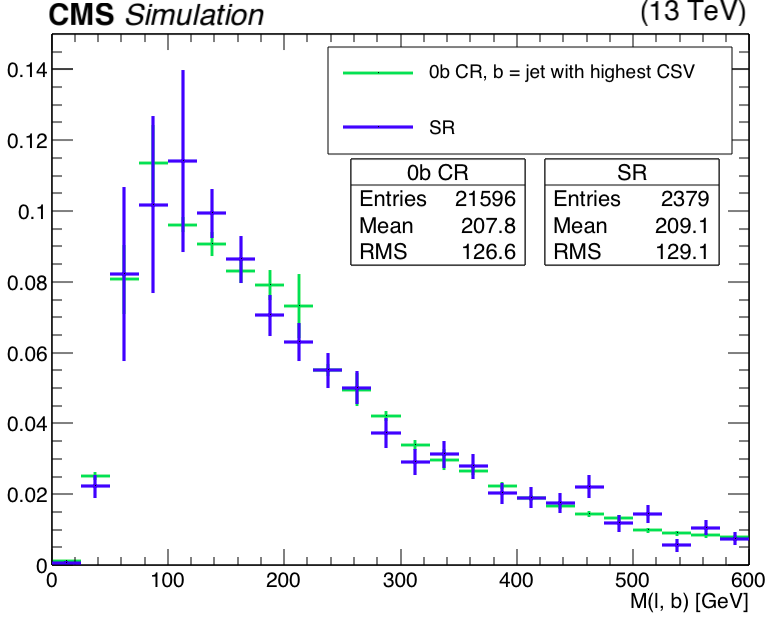
\includegraphics[width=0.4\textwidth]{figures/cr0b_Mlbshape_AB.png}
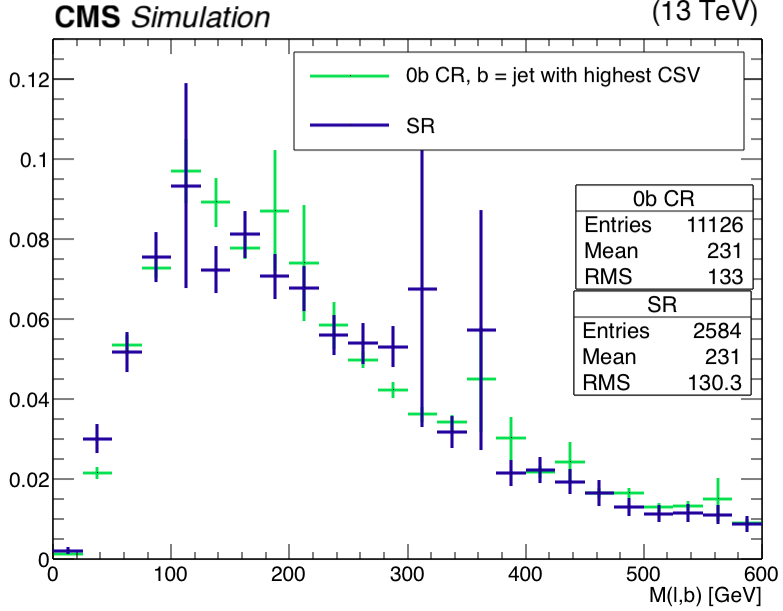
\includegraphics[width=0.4\textwidth]{figures/cr0b_Mlbshape_CD.png}
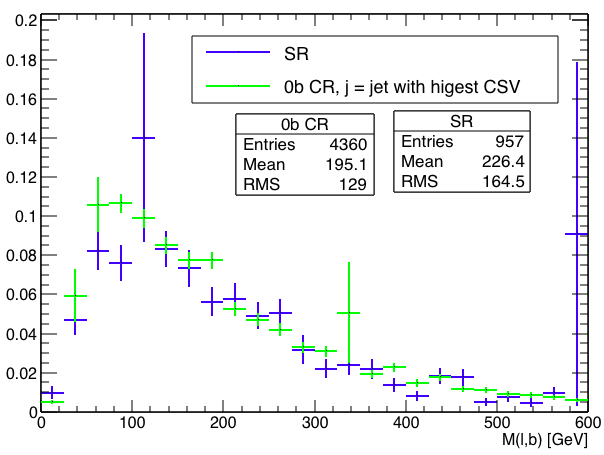
\includegraphics[width=0.4\textwidth]{figures/cr0b_Mlbshape_EF.png}
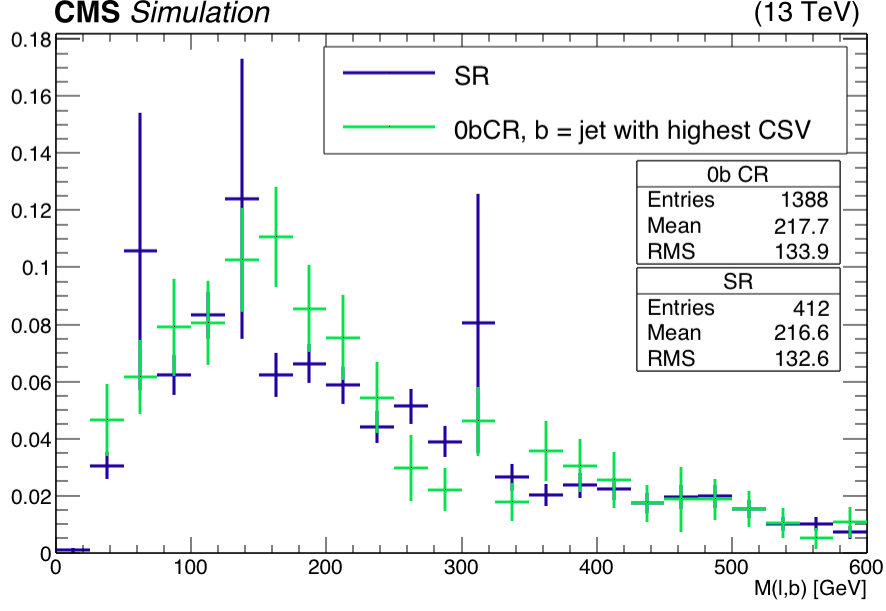
\includegraphics[width=0.4\textwidth]{figures/cr0b_Mlbshape_GH.png}
\caption{Comparison between $\mlb$ from SRs and makeshift $\mlb$
   from CRs, using simulated data. The four plots are made in the
  combined A+B regions, the C+D regions, the E+F regions, and the G+H
  regions, respectively.}
\label{fig:stop:1lw:mlb}
\end{figure}

\begin{figure}[htbp]
\centering
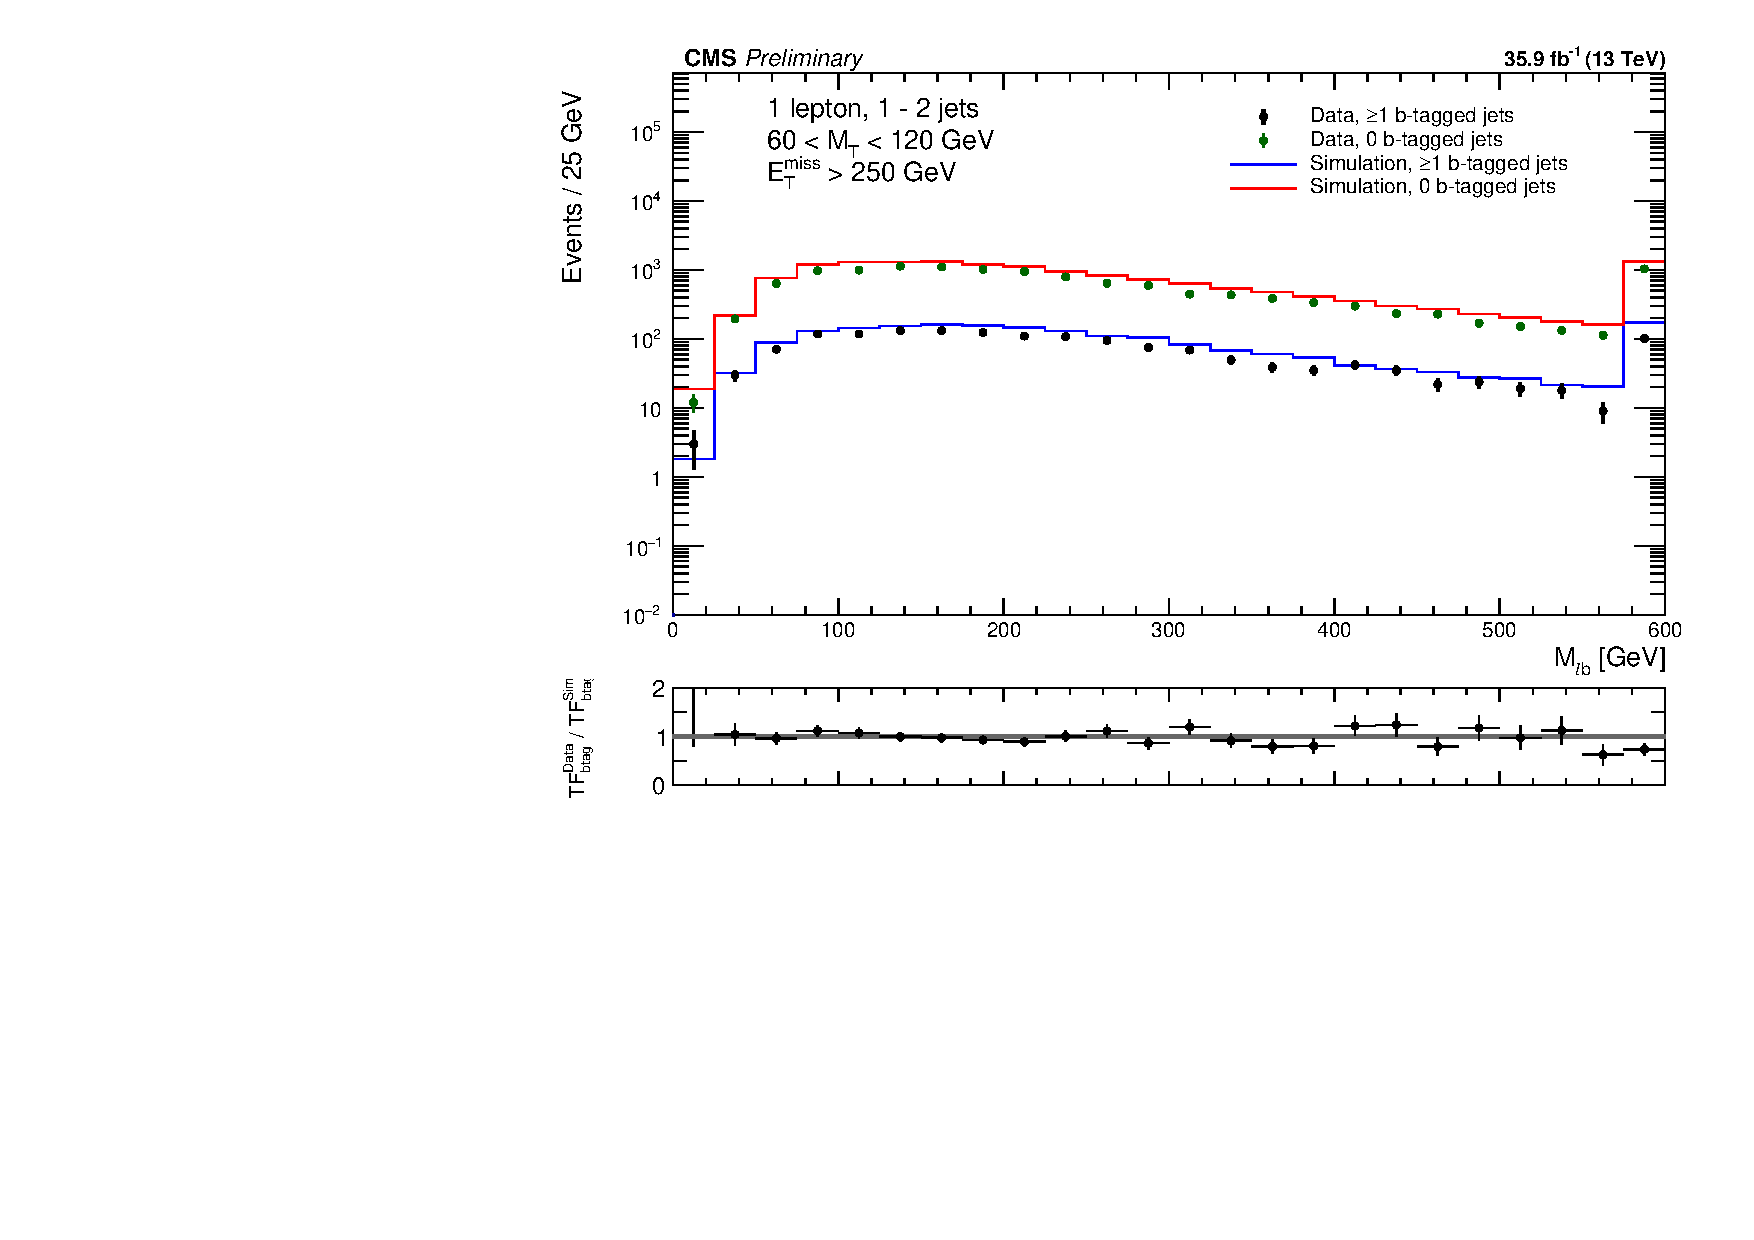
\includegraphics[width=0.8\textwidth]{figures/cr0b_Mlbshape_crosscheck.pdf}
\caption{Comparison of $\mlb$ shape for data and MC, in 0-btag
  and $\geq$1-btag crosscheck regions.}
\label{fig:stop:1lw:mlbxcheck}
\end{figure}

The yields for data and MC in the control regions are given in Table
\ref{tab:stop:1lw:cryields}. The MC simulations receive all the same
corrections as in the SRs. The purity of these control regions ranges
from a high of 83\% to a low of 37\%. The impurity of these regions
will be addressed further on with a systematic uncertainty.

% Yield table made by hand. Corridor results taken from common looper;
% bulk results scraped from tables in AN-16-463.
\begin{sidewaystable}
\centering
\scriptsize
\caption{Data and Monte Carlo yields in the 0-btag control regions,
  based on 35.9 fb\textsuperscript{-1} of luminosity.}
\label{tab:stop:1lw:cryields}
\begin{tabular}{|l|c c c c c|c|c|}
\hline
Region  & $\ge2$~leptons & $1$~lepton,~from~$W$ & $1$~lepton,~from~$t$ & $Z\rightarrow\nu\nu$ & Sum Bkg. & Data & Data/MC \\*
\hline \hline
$<4$ jets,~$\tmod \ge10$,~$\mlb<175$,~$250<\met<350$        & 31.59 $\pm$ 2.40 & 99.79 $\pm$ 3.00  & 0.49 $\pm$ 0.28 & 14.59 $\pm$ 2.05 & 146.46 $\pm$ 4.36 & 151 $\pm$ 12.29 & 1.03 $\pm$ 0.09 \\
$<4$ jets,~$\tmod \ge10$,~$\mlb<175$,~$350<\met<450$        & 10.15 $\pm$ 1.33 & 48.50 $\pm$ 2.25  & 0.33 $\pm$ 0.23 & 9.55 $\pm$ 1.40  & 68.52 $\pm$ 2.97  & 68 $\pm$ 8.25   & 0.99 $\pm$ 0.13 \\
$<4$ jets,~$\tmod \ge10$,~$\mlb<175$,~$450<\met<600$        & 3.44 $\pm$ 0.84  & 24.34 $\pm$ 1.79  &       ---       & 4.68 $\pm$ 1.08  & 32.45 $\pm$ 2.25  & 31 $\pm$ 5.57   & 0.96 $\pm$ 0.18 \\
$<4$ jets,~$\tmod \ge10$,~$\mlb<175$,~$\met>600$            & 0.39 $\pm$ 0.20  & 6.66 $\pm$ 0.37   &       ---       & 1.20 $\pm$ 0.53  & 8.25 $\pm$ 0.68   & 11 $\pm$ 3.32   & 1.33 $\pm$ 0.42 \\
\hline
$<4$ jets,~$\tmod \ge10$,~$\mlb\ge175$,~$250<\met<450$      & 19.15 $\pm$ 1.90 & 167.31 $\pm$ 1.88 &       ---       & 22.63 $\pm$ 2.37 & 209.09 $\pm$ 3.57 & 234 $\pm$ 15.30 & 1.12 $\pm$ 0.08 \\
$<4$ jets,~$\tmod \ge10$,~$\mlb\ge175$,~$450<\met<650$      & 3.22 $\pm$ 0.80  & 44.17 $\pm$ 1.46  &       ---       & 9.67 $\pm$ 1.44  & 57.06 $\pm$ 2.20  & 49 $\pm$ 7.00   & 0.86 $\pm$ 0.13 \\
$<4$ jets,~$\tmod \ge10$,~$\mlb\ge175$,~$\met>600$          & 0.40 $\pm$ 0.27  & 26.11 $\pm$ 1.76  &       ---       & 4.38 $\pm$ 1.10  & 30.89 $\pm$ 2.09  & 27 $\pm$ 5.20   & 0.87 $\pm$ 0.18 \\
\hline
$\ge4$ jets,~$\tmod <0.0$,~$\mlb<175$,~$250<\met<350$       & 81.70 $\pm$ 3.39 & 55.64 $\pm$ 2.31  & 5.02 $\pm$ 0.87 & 8.92 $\pm$ 1.19  & 151.28 $\pm$ 4.37 & 143 $\pm$ 11.96 & 0.95 $\pm$ 0.08 \\
$\ge4$ jets,~$\tmod <0.0$,~$\mlb<175$,~$350<\met<450$       & 16.78 $\pm$ 1.62 & 17.05 $\pm$ 1.69  & 0.53 $\pm$ 0.26 & 3.78 $\pm$ 0.88  & 38.14 $\pm$ 2.51  & 31 $\pm$ 5.57   & 0.81 $\pm$ 0.16 \\
$\ge4$ jets,~$\tmod <0.0$,~$\mlb<175$,~$450<\met<550$       & 4.27 $\pm$ 0.85  & 3.89 $\pm$ 0.28   & 0.17 $\pm$ 0.17 & 1.76 $\pm$ 0.61  & 10.08 $\pm$ 1.09  & 5 $\pm$ 2.24    & 0.50 $\pm$ 0.23 \\
$\ge4$ jets,~$\tmod <0.0$,~$\mlb<175$,~$550<\met<650$       & 0.84 $\pm$ 0.33  & 1.66 $\pm$ 0.25   &       ---       & 0.09 $\pm$ 0.02  & 2.59 $\pm$ 0.41   & 3 $\pm$ 1.73    & 1.16 $\pm$ 0.69 \\
$\ge4$ jets,~$\tmod <0.0$,~$\mlb<175$,~$\met>650$           & 0.97 $\pm$ 0.40  & 1.18 $\pm$ 0.15   & 0.13 $\pm$ 0.13 & 0.32 $\pm$ 0.27  & 2.60 $\pm$ 0.52   & 4 $\pm$ 2.00    & 1.54 $\pm$ 0.83 \\
\hline
$\ge4$ jets,~$\tmod <0.0$,~$\mlb\ge175$,~$250<\met<350$     & 36.35 $\pm$ 2.31 & 81.05 $\pm$ 3.77  & 2.58 $\pm$ 0.59 & 6.82 $\pm$ 1.28  & 126.80 $\pm$ 4.64 & 104 $\pm$ 10.20 & 0.82 $\pm$ 0.09 \\
$\ge4$ jets,~$\tmod <0.0$,~$\mlb\ge175$,~$350<\met<450$     & 10.93 $\pm$ 1.30 & 31.43 $\pm$ 3.80  & 0.42 $\pm$ 0.24 & 5.69 $\pm$ 1.05  & 48.47 $\pm$ 4.15  & 27 $\pm$ 5.20   & 0.56 $\pm$ 0.12 \\
$\ge4$ jets,~$\tmod <0.0$,~$\mlb\ge175$,~$450<\met<550$     & 3.77 $\pm$ 0.78  & 10.41 $\pm$ 0.51  & 0.00 $\pm$ 0.00 & 1.57 $\pm$ 0.67  & 15.74 $\pm$ 1.15  & 9 $\pm$ 3.00    & 0.57 $\pm$ 0.20 \\
$\ge4$ jets,~$\tmod <0.0$,~$\mlb\ge175$,~$\met>550$         & 3.99 $\pm$ 1.36  & 8.50 $\pm$ 0.45   & 0.13 $\pm$ 0.13 & 1.23 $\pm$ 0.58  & 13.84 $\pm$ 1.55  & 12 $\pm$ 3.46   & 0.87 $\pm$ 0.27 \\
\hline
$\ge4$ jets,~$0.0< \tmod <10$,~$\mlb<175$,~$250<\met<350$  & 16.96 $\pm$ 1.51 & 28.65 $\pm$ 3.66  & 0.29 $\pm$ 0.21 & 4.87 $\pm$ 0.81  & 50.78 $\pm$ 4.05  & 54 $\pm$ 7.35   & 1.06 $\pm$ 0.17 \\
$\ge4$ jets,~$0.0< \tmod <10$,~$\mlb<175$,~$350<\met<550$  & 4.17 $\pm$ 0.80  & 12.99 $\pm$ 0.53  & 0.12 $\pm$ 0.12 & 1.71 $\pm$ 0.63  & 19.00 $\pm$ 1.15  & 13 $\pm$ 3.61   & 0.68 $\pm$ 0.19 \\
$\ge4$ jets,~$0.0< \tmod <10$,~$\mlb<175$,~$\met>550$      & 0.32 $\pm$ 0.18  & 1.38 $\pm$ 0.16   &       ---       & 0.75 $\pm$ 0.41  & 2.45 $\pm$ 0.48   & 2 $\pm$ 1.41    & 0.82 $\pm$ 0.60 \\
\hline
$\ge4$ jets,~$0.0< \tmod <10$,~$\mlb\ge175$,~$250<\met<450$& 6.60 $\pm$ 0.90  & 34.16 $\pm$ 1.52  &       ---       & 5.12 $\pm$ 0.96  & 45.88 $\pm$ 2.01  & 51 $\pm$ 7.14   & 1.11 $\pm$ 0.16 \\
$\ge4$ jets,~$0.0< \tmod <10$,~$\mlb\ge175$,~$\met>450$    & 1.68 $\pm$ 0.81  & 8.35 $\pm$ 0.40   &       ---       & 2.54 $\pm$ 0.63  & 12.58 $\pm$ 1.10  & 5 $\pm$ 2.24    & 0.40 $\pm$ 0.18 \\
\hline
$\ge4$ jets,~$\tmod \ge10$,~$\mlb<175$,~$250<\met<350$      & 1.83 $\pm$ 0.47  & 1.82 $\pm$ 0.19   & 0.16 $\pm$ 0.16 & 0.58 $\pm$ 0.24  & 4.38 $\pm$ 0.58   & 8 $\pm$ 2.83    & 1.82 $\pm$ 0.69 \\
$\ge4$ jets,~$\tmod \ge10$,~$\mlb<175$,~$350<\met<450$      & 1.98 $\pm$ 0.52  & 3.88 $\pm$ 1.13   &       ---       & 0.26 $\pm$ 0.03  & 6.11 $\pm$ 1.24   & 7 $\pm$ 2.65    & 1.15 $\pm$ 0.49 \\
$\ge4$ jets,~$\tmod \ge10$,~$\mlb<175$,~$450<\met<600$      & 1.42 $\pm$ 0.57  & 2.96 $\pm$ 0.24   &       ---       & 0.52 $\pm$ 0.44  & 4.89 $\pm$ 0.76   & 3 $\pm$ 1.73    & 0.61 $\pm$ 0.37 \\
$\ge4$ jets,~$\tmod \ge10$,~$\mlb<175$,~$\met>600$          & 0.68 $\pm$ 0.39  & 2.54 $\pm$ 1.16   &       ---       & 0.32 $\pm$ 0.45  & 3.54 $\pm$ 1.30   & 2 $\pm$ 1.41    & 0.57 $\pm$ 0.45 \\
\hline
$\ge4$ jets,~$\tmod \ge10$,~$\mlb\ge175$,~$250<\met<450$    & 2.04 $\pm$ 0.84  & 6.03 $\pm$ 0.34   & 0.11 $\pm$ 0.11 & 0.41 $\pm$ 0.14  & 8.60 $\pm$ 0.92   & 10 $\pm$ 3.16   & 1.16 $\pm$ 0.39 \\
$\ge4$ jets,~$\tmod \ge10$,~$\mlb\ge175$,~$\met>450$        & 0.93 $\pm$ 0.45  & 8.10 $\pm$ 0.39   &       ---       & 2.14 $\pm$ 0.53  & 11.17 $\pm$ 0.80  & 7 $\pm$ 2.65    & 0.63 $\pm$ 0.24 \\
\hline
Compressed search, $250<\met<350$  & 19.70 $\pm$ 1.43  & 23.62 $\pm$ 4.24  & 1.80 $\pm$ 0.45  & 2.36 $\pm$ 0.52  & 47.47 $\pm$ 4.53  & 49 $\pm$ 7.00  & 1.03 $\pm$ 0.18 \\*
Compressed search, $350<\met<450$  & 7.49 $\pm$ 0.92  & 12.07 $\pm$ 3.64  & 0.40 $\pm$ 0.21  & 2.43 $\pm$ 0.76  & 22.38 $\pm$ 3.83  & 11 $\pm$ 3.32  & 0.49 $\pm$ 0.17 \\*
Compressed search, $450<\met<550$  & 2.98 $\pm$ 0.67  & 3.68 $\pm$ 0.27  & 0.30 $\pm$ 0.22  & 1.75 $\pm$ 0.53  & 8.71 $\pm$ 0.92  & 5 $\pm$ 2.24  & 0.57 $\pm$ 0.26 \\*
Compressed search, $\met>550$      & 1.43 $\pm$ 0.43  & 3.26 $\pm$ 0.26  & ---  & 1.13 $\pm$ 0.48  & 5.82 $\pm$ 0.70  & 3 $\pm$ 1.73  & 0.52 $\pm$ 0.30 \\*
\hline
\end{tabular}
\end{sidewaystable}

\subsubsection{Systematic Uncertainties}
\label{sssec:stop:1lw:systematics}

Many of the systematic uncertainties on the 1$\ell$W background are
assessed the same way as for the lost lepton background, as described
in Section \ref{sssec:stop:lostlep:systematics}. These uncertainties
are:
\begin{itemize}
\item Data and MC statistics
\item b-tagging efficiencies
\item JES
\item PDF
\item $Q^2$
\end{itemize}

Because our $TF_\text{btag}$ is derived from simulation, we must ensure that
the relative cross-sections of W+b and W+non-b jets are correctly
modeled in MC. We check the agreement between data and MC on number of
b-jets in the high-statistics crosscheck region described above. As
Figure \ref{fig:stop:1lw:wb} shows, a 50\% systematic uncertainty on
the W+b cross section adequately covers any mismodeling that may
exist. Additionally, the 0-btag CRs have considerable impurity from
non-1$\ell$W backgrounds, so we assess a 50\% systematic uncertainty on
that contamination. The systematic uncertainties on the single lepton
from W estimate are presented in Table \ref{tab:stop:1lw:systematics}.

% Plot of W+b crosscheck, taken from AN-16-463.
\begin{figure}[htb]
\centering
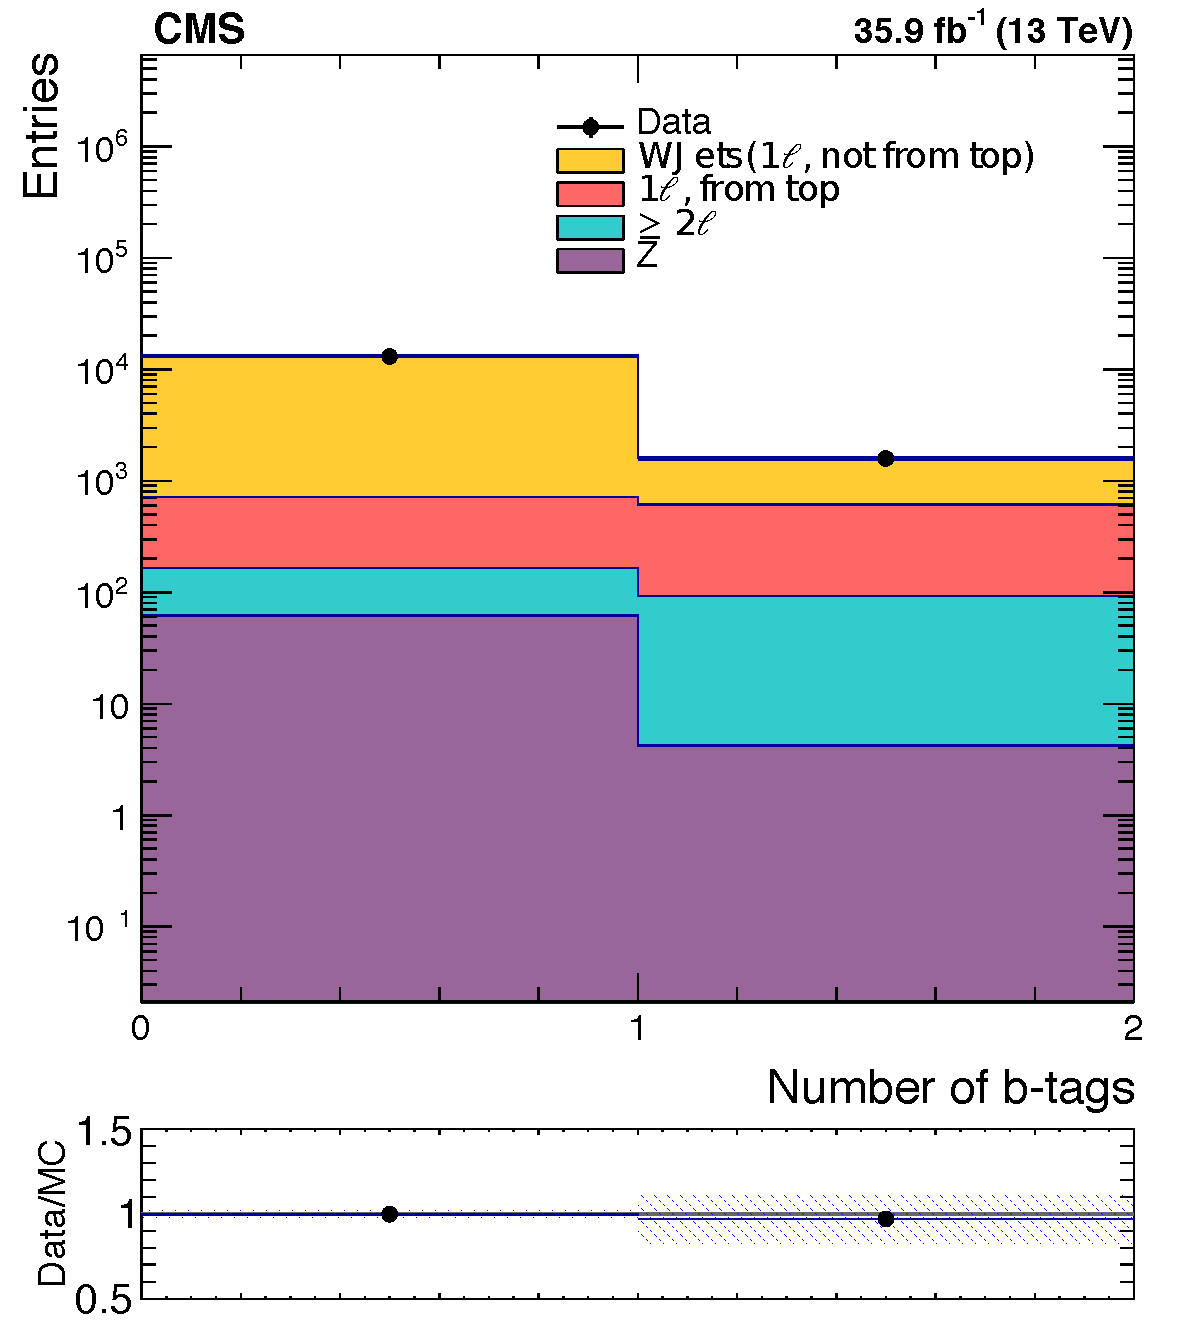
\includegraphics[width=0.45\textwidth]{figures/cr0b_nbtags_crosscheck.pdf}
\caption{Number of b-tags compared between data and MC, in
  high-statistics crosscheck region. The second bin includes events
  with one or more b-tags. The uncertainty band illustrates a 50\%
  uncertainty on the W+b cross section}
\label{fig:stop:1lw:wb}
\end{figure}

% Systematics table made by me. Nominal systematics derived from
% Indara's histograms; corridor systematics obtained from the common looper.
\begin{sidewaystable}
\centering
\small
\caption{Summary of systematic uncertainties on single lepton from W
  background estimate.}
\label{tab:stop:1lw:systematics}
\begin{tabular}{| l | c c | c c c c c c c | c |}
\hline
Region & Data Stats & MC Stats & CR Impurity & JES & W+b X-sec & b-tag (HF) & b-tag (LF) & $Q^2$ & PDF & Total \\
\hline
 A  $250 < \met < 350$  &   9.2\% &   6.1\% &  23.4\% &   2.0\% &  22.8\% &   1.7\% &   2.5\% &   0.1\% &   1.0\% &  34.7\% \\
 A  $350 < \met < 450$  &  13.7\% &   8.5\% &  20.6\% &   2.0\% &  21.0\% &   1.5\% &   3.1\% &   0.1\% &   0.6\% &  33.8\% \\
 A  $450 < \met < 600$  &  20.6\% &  13.0\% &  16.7\% &   2.0\% &  25.1\% &   1.3\% &   2.9\% &   0.1\% &   1.0\% &  39.0\% \\
 A  $\met >600$  &  31.7\% &  21.0\% &  11.9\% &   2.0\% &  15.2\% &   0.9\% &   5.1\% &   0.2\% &   2.0\% &  43.1\% \\
\hline
 B  $250 < \met < 450$  &   6.8\% &   6.7\% &  12.5\% &   2.0\% &  35.6\% &   2.2\% &   2.7\% &   0.6\% &   0.7\% &  39.2\% \\
 B  $450 < \met < 600$  &  15.2\% &  11.0\% &  14.6\% &   2.0\% &  32.5\% &   2.5\% &   2.0\% &   1.4\% &   1.7\% &  40.5\% \\
 B  $\met >600$  &  21.5\% &  15.4\% &   9.2\% &   2.0\% &  35.6\% &   4.1\% &   1.7\% &   0.1\% &   1.0\% &  45.5\% \\
\hline
 C  $250 < \met < 350$  &   9.8\% &  12.6\% &  85.9\% &   2.0\% &  17.5\% &   1.5\% &   2.3\% &   0.7\% &   0.5\% &  89.2\% \\
 C  $350 < \met < 450$  &  21.5\% &  15.8\% &  61.8\% &   2.0\% &  17.5\% &   1.1\% &   2.9\% &   0.8\% &   1.6\% &  69.7\% \\
 C  $450 < \met < 550$  &  46.6\% &  21.3\% &  79.6\% &   2.0\% &  23.0\% &   0.6\% &   2.0\% &   2.2\% &   0.8\% &  97.5\% \\
 C  $550 < \met < 650$  &  61.7\% &  32.2\% &  28.1\% &   2.0\% &  15.7\% &   1.4\% &   4.3\% &   1.1\% &   1.6\% &  76.9\% \\
 C  $\met >650$  &  55.3\% &  30.7\% &  60.7\% &   2.0\% &  12.1\% &   1.0\% &   1.7\% &   6.9\% &   9.2\% &  89.3\% \\
\hline
 D  $250 < \met < 350$  &  11.5\% &   9.3\% &  28.2\% &   2.0\% &  23.3\% &   2.3\% &   2.0\% &   3.2\% &   1.7\% &  39.8\% \\
 D  $350 < \met < 450$  &  24.3\% &  17.6\% &  27.1\% &   2.0\% &  24.0\% &   2.1\% &   2.0\% &   3.6\% &   2.3\% &  47.4\% \\
 D  $450 < \met < 550$  &  34.5\% &  23.1\% &  25.6\% &   2.0\% &  30.4\% &   2.2\% &   1.2\% &   1.1\% &   0.6\% &  57.6\% \\
 D  $\met >550$  &  31.4\% &  26.8\% &  31.5\% &   2.0\% &  18.0\% &   2.3\% &   1.9\% &   6.6\% &   6.1\% &  55.8\% \\
\hline
 E  $250 < \met < 350$  &  20.3\% &  25.0\% &  38.6\% &   2.0\% &  17.4\% &   2.1\% &   2.0\% &   2.7\% &   1.9\% &  53.4\% \\
 E  $350 < \met < 550$  &  28.7\% &  10.9\% &  23.1\% &   2.0\% &  18.9\% &   1.7\% &   2.8\% &   0.9\% &   1.3\% &  43.0\% \\
 E  $\met >550$  &  74.3\% &  26.9\% &  39.1\% &   2.0\% &  29.9\% &   0.8\% &   3.6\% &   0.7\% &   0.4\% &  93.2\% \\
\hline
 F  $250 < \met < 450$  &  15.3\% &  11.4\% &  17.2\% &   2.0\% &  32.4\% &   2.1\% &   1.1\% &   0.1\% &   0.1\% &  41.5\% \\
 F  $\met >450$  &  45.8\% &  18.6\% &  25.3\% &   2.0\% &  33.2\% &   2.2\% &   2.2\% &   2.5\% &   3.1\% &  65.0\% \\
\hline
 G  $250 < \met < 350$  &  39.1\% &  20.7\% &  70.5\% &   2.0\% &  22.1\% &   1.4\% &   1.8\% &   1.5\% &   5.9\% &  86.5\% \\
 G  $350 < \met < 450$  &  51.8\% &  33.8\% &  28.8\% &   2.0\% &  23.9\% &   1.3\% &   2.1\% &   3.1\% &   2.8\% &  72.5\% \\
 G  $450 < \met < 600$  &  60.3\% &  18.0\% &  32.7\% &   2.0\% &  21.6\% &   1.3\% &   4.1\% &   0.5\% &   1.4\% &  74.4\% \\
 G  $\met >600$  &  91.9\% &  49.1\% &  19.8\% &   2.0\% &  25.5\% &   1.4\% &   2.9\% &   5.6\% &   3.6\% & 109.3\% \\
\hline
 H  $250 < \met < 450$  &  33.8\% &  16.0\% &  21.3\% &   2.0\% &  40.4\% &   1.9\% &   1.2\% &   0.7\% &   0.1\% &  59.2\% \\
 H  $\met >450$  &  38.8\% &  16.7\% &  19.0\% &   2.0\% &  35.2\% &   2.6\% &   2.3\% &   3.5\% &   0.1\% &  58.4\% \\
\hline
 I  $250 < \met < 350$  & 14.3\%  & 27.3\%  & 33.6\%  & 5.9\%  & 8.2\%  & 2.2\%  & 5.3\%  & 1.4\%  & 2.8\%  & 33.1\%  \\
 I  $350 < \met < 450$  & 30.2\%  & 19.6\%  & 29.9\%  & 6.8\%  & 4.3\%  & 3.0\%  & 2.7\%  & 3.3\%  & 9.6\%  & 38.4\%  \\
 I  $450 < \met < 550$  & 44.7\%  & 23.0\%  & 40.6\%  & 6.2\%  & 14.8\%  & 2.6\%  & 2.4\%  & 7.2\%  & 14.4\%  & 55.3\%  \\
 I  $\met >550$ & 57.7\% & 23.2\% & 28.2\% & 4.5\% & 24.6\% & 3.1\% & 2.9\% & 5.4\% & 14.0\% & 68.9\% \\
\hline
\end{tabular}
\end{sidewaystable}

\subsubsection{Results}
\label{sssec:stop:1lw:results}

The full results of the single lepton from W background estimate,
including systematic uncertainties, are presented in Table
\ref{tab:stop:1lw:results}.

% 1lW estimate results. Corridor numbers made using common looper,
% bulk numbers scraped from tables in AN-16-463.
\begin{sidewaystable}
\centering
\small
\caption{Summary of the single lepton from W background estimate, and
  all its key components.}
\label{tab:stop:1lw:results}
\begin{tabular}{|l|c|c|c|c|c|} \hline
Region & $\met$ bin & Observed$_\text{CR}$ & Purity & $TF_\text{btag}$ & SR Estimate \\ \hline \hline
 $<4$ jets,~$\tmod \ge10.0$,~$\mlb <175$        & $250<\met<350$ & 151 $\pm$ 12.29 & 0.68 $\pm$ 0.03  & 0.07 $\pm$ 0.00 & 7.18 $\pm$ 0.79 \\
 $<4$ jets,~$\tmod \ge10.0$,~$\mlb <175$        & $350<\met<450$ & 68 $\pm$ 8.25   & 0.71 $\pm$ 0.04  & 0.08 $\pm$ 0.01 & 4.06 $\pm$ 0.65 \\
 $<4$ jets,~$\tmod \ge10.0$,~$\mlb <175$        & $450<\met<600$ & 31 $\pm$ 5.57   & 0.75 $\pm$ 0.08  & 0.07 $\pm$ 0.01 & 1.71 $\pm$ 0.42 \\
 $<4$ jets,~$\tmod \ge10.0$,~$\mlb <175$        & $\met>600$     & 11 $\pm$ 3.32   & 0.81 $\pm$ 0.08  & 0.09 $\pm$ 0.02 & 0.78 $\pm$ 0.30 \\
\hline
 $<4$ jets,~$\tmod \ge10.0$,~$\mlb \ge175$      & $250<\met<450$ & 234 $\pm$ 15.30 & 0.80 $\pm$ 0.02  & 0.03 $\pm$ 0.00 & 5.64 $\pm$ 0.54 \\
 $<4$ jets,~$\tmod \ge10.0$,~$\mlb \ge175$      & $450<\met<600$ & 49 $\pm$ 7.00   & 0.77 $\pm$ 0.04  & 0.04 $\pm$ 0.00 & 1.56 $\pm$ 0.29 \\
 $<4$ jets,~$\tmod \ge10.0$,~$\mlb \ge175$      & $\met>600$     & 27 $\pm$ 5.20   & 0.85 $\pm$ 0.08  & 0.04 $\pm$ 0.01 & 0.87 $\pm$ 0.23 \\
\hline
 $\ge4$ jets,~$\tmod <0.0$,~$\mlb <175$         & $250<\met<350$ & 143 $\pm$ 11.96 & 0.37 $\pm$ 0.02  & 0.18 $\pm$ 0.02 & 9.65 $\pm$ 1.54 \\
 $\ge4$ jets,~$\tmod <0.0$,~$\mlb <175$         & $350<\met<450$ & 31 $\pm$ 5.57   & 0.45 $\pm$ 0.05  & 0.18 $\pm$ 0.03 & 2.51 $\pm$ 0.67 \\
 $\ge4$ jets,~$\tmod <0.0$,~$\mlb <175$         & $450<\met<550$ & 5 $\pm$ 2.24    & 0.39 $\pm$ 0.05  & 0.25 $\pm$ 0.05 & 0.47 $\pm$ 0.24 \\
 $\ge4$ jets,~$\tmod <0.0$,~$\mlb <175$         & $550<\met<650$ & 3 $\pm$ 1.73    & 0.64 $\pm$ 0.14  & 0.14 $\pm$ 0.04 & 0.26 $\pm$ 0.18 \\
 $\ge4$ jets,~$\tmod <0.0$,~$\mlb <175$         & $\met>650$     & 4 $\pm$ 2.00    & 0.45 $\pm$ 0.11  & 0.24 $\pm$ 0.07 & 0.43 $\pm$ 0.27 \\
\hline
 $\ge4$ jets,~$\tmod <0.0$,~$\mlb \ge175$       & $250<\met<350$ & 104 $\pm$ 10.20 & 0.64 $\pm$ 0.04  & 0.11 $\pm$ 0.01 & 7.52 $\pm$ 1.11 \\
 $\ge4$ jets,~$\tmod <0.0$,~$\mlb \ge175$       & $350<\met<450$ & 27 $\pm$ 5.20   & 0.65 $\pm$ 0.10  & 0.09 $\pm$ 0.02 & 1.55 $\pm$ 0.47 \\
 $\ge4$ jets,~$\tmod <0.0$,~$\mlb \ge175$       & $450<\met<550$ & 9 $\pm$ 3.00    & 0.66 $\pm$ 0.06  & 0.09 $\pm$ 0.02 & 0.56 $\pm$ 0.23 \\
 $\ge4$ jets,~$\tmod <0.0$,~$\mlb \ge175$       & $\met>550$     & 12 $\pm$ 3.46   & 0.61 $\pm$ 0.08  & 0.14 $\pm$ 0.04 & 1.02 $\pm$ 0.42 \\
\hline
 $\ge4$ jets,~$0.0<$tmod$<10.0$,~$\mlb <175$  & $250<\met<350$ & 54 $\pm$ 7.35   & 0.56 $\pm$ 0.09  & 0.19 $\pm$ 0.05 & 5.67 $\pm$ 1.83 \\
 $\ge4$ jets,~$0.0<$tmod$<10.0$,~$\mlb <175$  & $350<\met<550$ & 13 $\pm$ 3.61   & 0.68 $\pm$ 0.05  & 0.14 $\pm$ 0.02 & 1.25 $\pm$ 0.38 \\
 $\ge4$ jets,~$0.0<$tmod$<10.0$,~$\mlb <175$  & $\met>550$     & 2 $\pm$ 1.41    & 0.56 $\pm$ 0.13  & 0.23 $\pm$ 0.06 & 0.26 $\pm$ 0.21 \\
\hline
 $\ge4$ jets,~$0.0<$tmod$<10.0$,~$\mlb \ge175$& $250<\met<450$ & 51 $\pm$ 7.14   & 0.74 $\pm$ 0.05  & 0.08 $\pm$ 0.01 & 3.10 $\pm$ 0.59 \\
 $\ge4$ jets,~$0.0<$tmod$<10.0$,~$\mlb \ge175$& $\met>450$     & 5 $\pm$ 2.24    & 0.66 $\pm$ 0.07  & 0.07 $\pm$ 0.01 & 0.24 $\pm$ 0.12 \\
\hline
 $\ge4$ jets,~$\tmod \ge10.0$,~$\mlb <175$      & $250<\met<350$ & 8 $\pm$ 2.83    & 0.41 $\pm$ 0.07  & 0.32 $\pm$ 0.07 & 1.06 $\pm$ 0.47 \\
 $\ge4$ jets,~$\tmod \ge10.0$,~$\mlb <175$      & $350<\met<450$ & 7 $\pm$ 2.65    & 0.63 $\pm$ 0.22  & 0.16 $\pm$ 0.05 & 0.71 $\pm$ 0.44 \\
 $\ge4$ jets,~$\tmod \ge10.0$,~$\mlb <175$      & $450<\met<600$ & 3 $\pm$ 1.73    & 0.60 $\pm$ 0.11  & 0.24 $\pm$ 0.04 & 0.43 $\pm$ 0.27 \\
 $\ge4$ jets,~$\tmod \ge10.0$,~$\mlb <175$      & $\met>600$     & 2 $\pm$ 1.41    & 0.72 $\pm$ 0.42  & 0.24 $\pm$ 0.12 & 0.34 $\pm$ 0.36 \\
\hline
 $\ge4$ jets,~$\tmod \ge10.0$,~$\mlb \ge175$    & $250<\met<450$ & 10 $\pm$ 3.16   & 0.70 $\pm$ 0.08  & 0.14 $\pm$ 0.02 & 1.00 $\pm$ 0.37 \\
 $\ge4$ jets,~$\tmod \ge10.0$,~$\mlb \ge175$    & $\met>450$     & 7 $\pm$ 2.65    & 0.72 $\pm$ 0.06  & 0.09 $\pm$ 0.02 & 0.46 $\pm$ 0.19 \\
\hline
Compressed search & $250<\met<350$  & 49 $\pm$ 7.00  & 0.50 $\pm$ 0.19  & 0.21 $\pm$ 0.06  & 5.03 $\pm$ 1.78  \\
Compressed search & $350<\met<450$  & 11 $\pm$ 3.32  & 0.54 $\pm$ 0.20  & 0.14 $\pm$ 0.03  & 0.84 $\pm$ 0.33  \\
Compressed search & $450<\met<550$  & 5 $\pm$ 2.24   & 0.42 $\pm$ 0.19  & 0.20 $\pm$ 0.05  & 0.42 $\pm$ 0.24  \\
Compressed search & $\met>550$      & 3 $\pm$ 1.73  & 0.56 $\pm$ 0.19  & 0.14 $\pm$ 0.05  & 0.24 $\pm$ 0.17  \\
\hline
\end{tabular}
\end{sidewaystable}

\subsection{Single Lepton from Top}
\label{ssec:stop:1ltop}

At the start of our search, before making any cuts to the data, the
main background to contend with was genuine single leptons that result
from top quarks decaying to W-bosons, which in turn decay
leptonically. However, as earlier sections have mentioned, our high
$\met$ and $\mt$ requirements are extremely effective at reducing this
background component. So much so, in fact, that after event
selections, the single lepton from top background (or 1$\ell$top) becomes
practically negligible in all our signal regions.

Unfortunately, there is no way to perform a robust, data-driven
estimate of this background, because we cannot construct a control
region that is enhanced in 1$\ell$top processes (mostly $\ttonelep$,
followed by single top quark production). Since this background was so
strongly reduced by the $\mt$ cut, one might consider a lower-$\mt$
sideband region; however, as we discovered in the previous section,
such a region contains a considerable number of 1$\ell$W events, and
even lost lepton events. Therefore, we are forced to estimate the
1$\ell$top background directly from Monte Carlo simulation.

As mentioned in Section \ref{sec:stop:searchstrategy}, most 1$\ell$top
events that pass the $\mt$ cut do so because of $\met$ resolution
effects. Therefore, by far the most dominant uncertainty on the 1$\ell
t$ background component is the uncertainty on $\met$ resolution. Our
studies in Appendix \ref{apx:stop:metres} show this uncertainty can be as high as 25\%. In
Figure \ref{fig:stop:1ltop:metres}, we show the $\met$ spectra of
$\ttonelep$ events from Monte Carlo, both before and after fluctuating
the $\met$ resolution according to the uncertainties from
Appendix \ref{apx:stop:metres}. We note that the yields in the various bins may fluctuate
enormously as the $\met$ resolution is varied within a realistic range. On that
basis, we assign a flat 100\% uncertainty to the 1$\ell$top background
component. All other uncertainties, including statistical, are
insignificant by comparison, and should be covered by the 100\%
uncertainty we impose.

% MET resolution fluctuation plots, from AN-16-463.
\begin{figure}
\centering
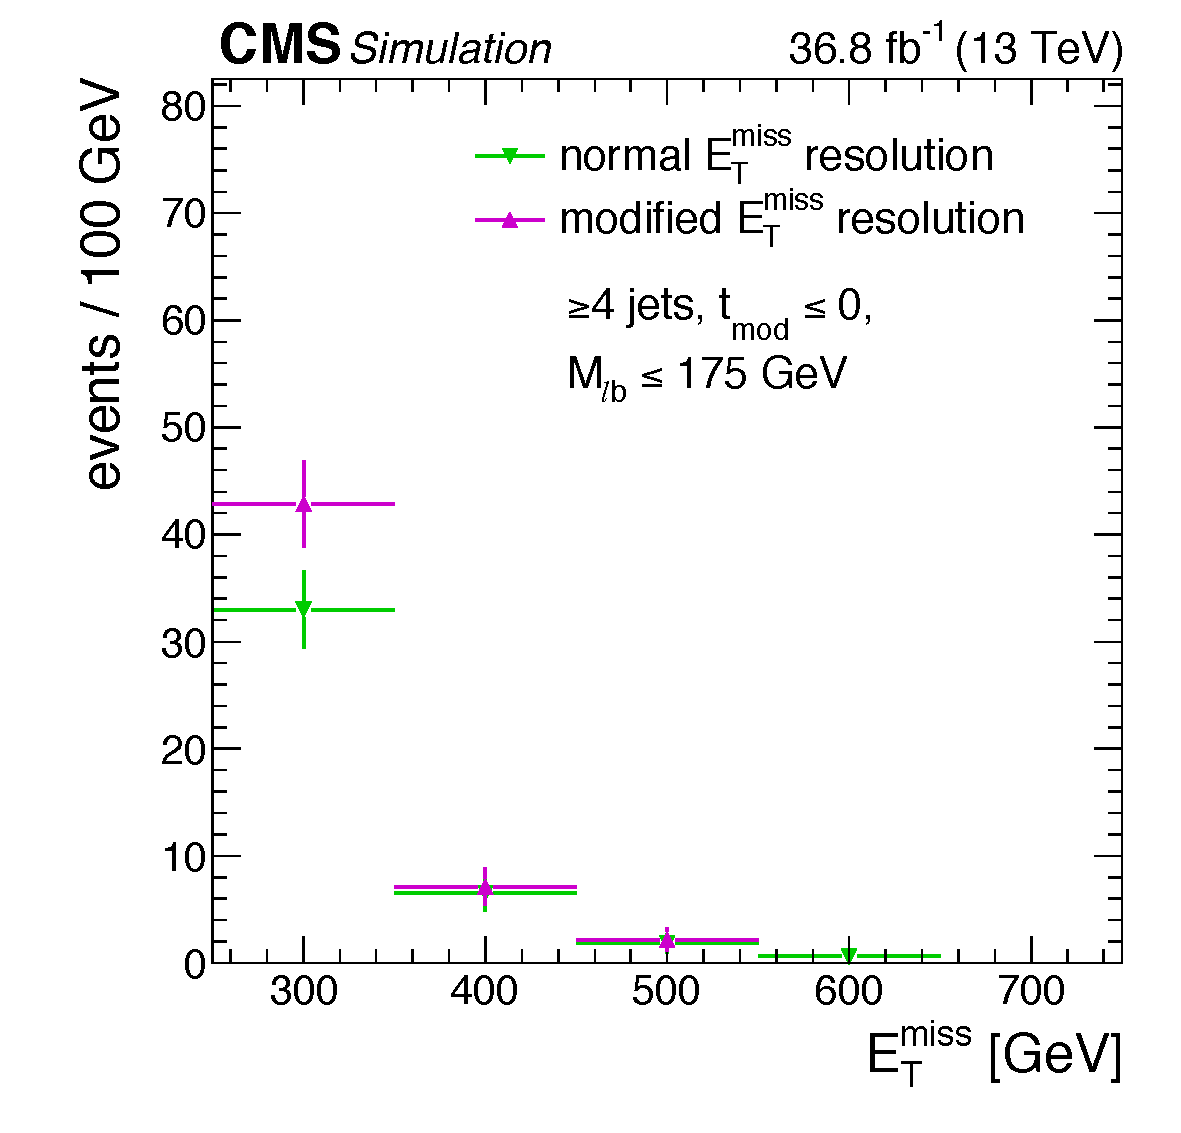
\includegraphics[width=0.45\textwidth]{figures/metres_1ltop_C.pdf}
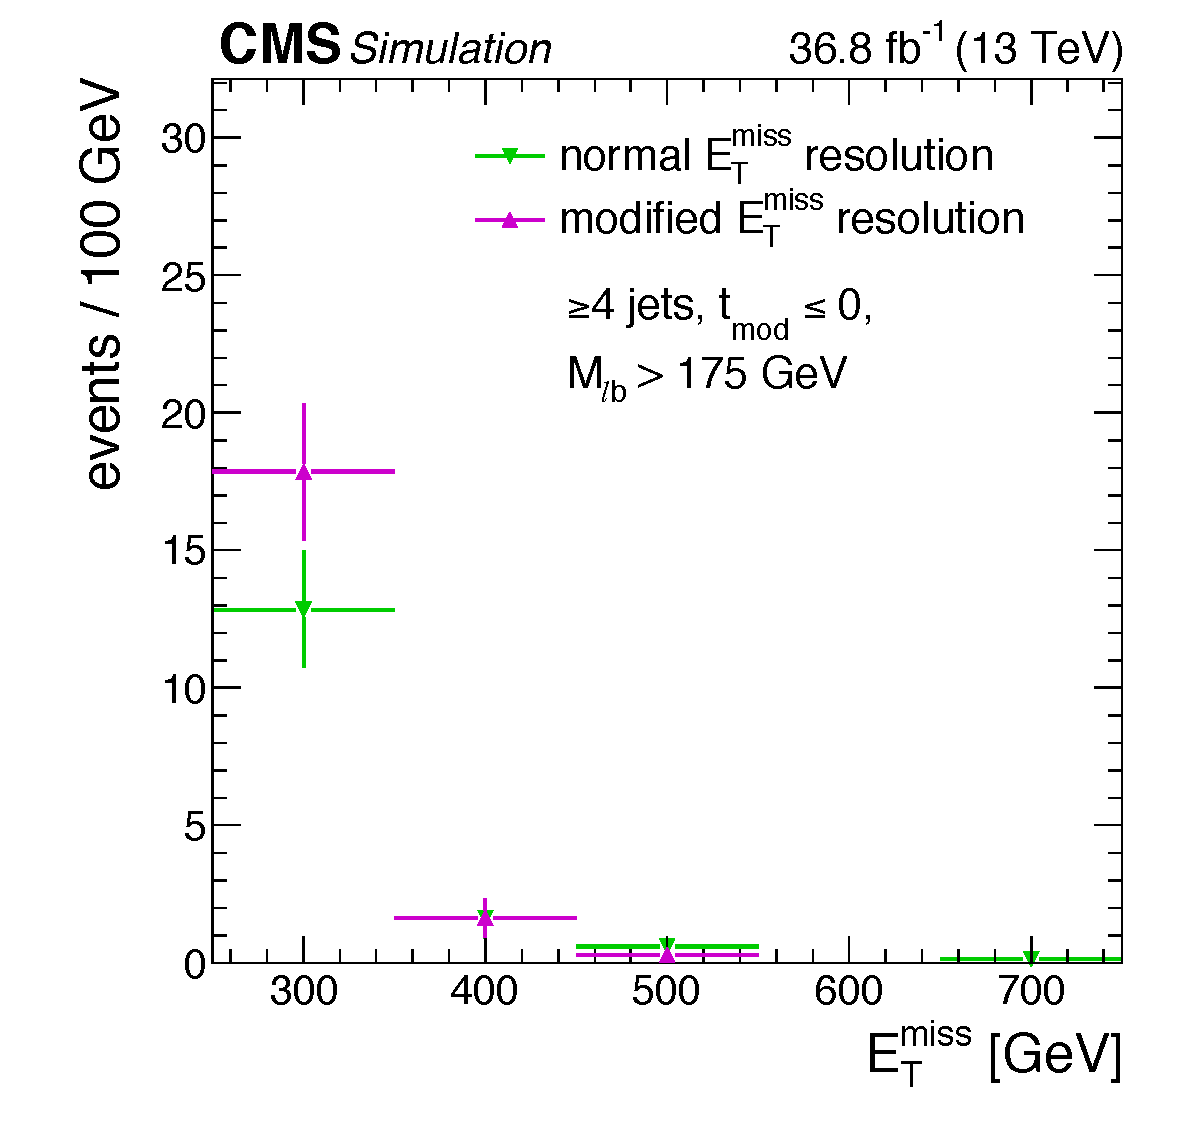
\includegraphics[width=0.45\textwidth]{figures/metres_1ltop_D.pdf}
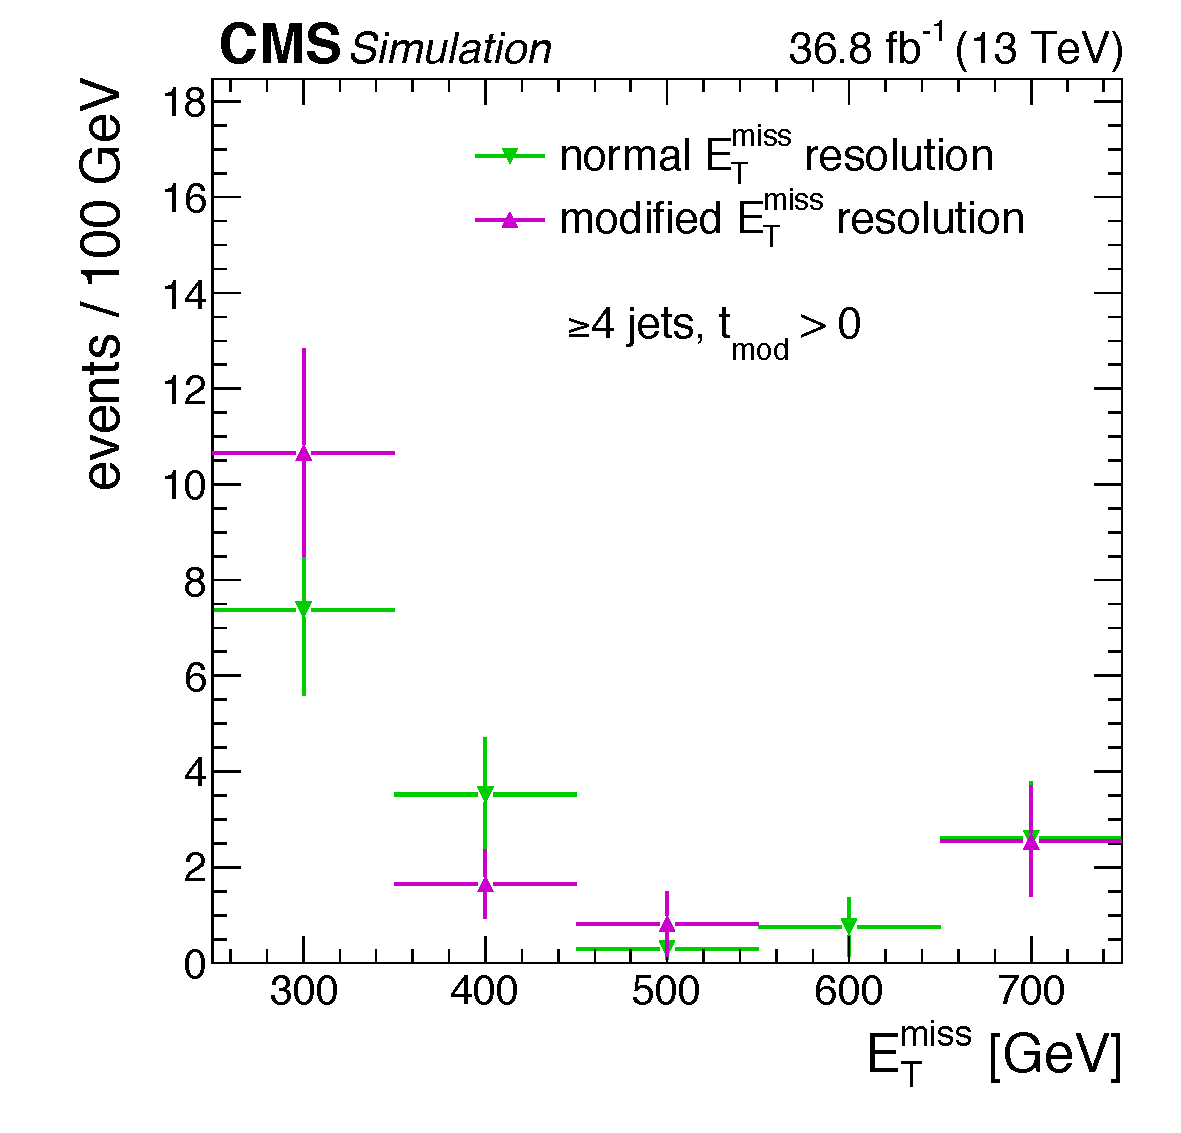
\includegraphics[width=0.45\textwidth]{figures/metres_1ltop_EFGH.pdf}
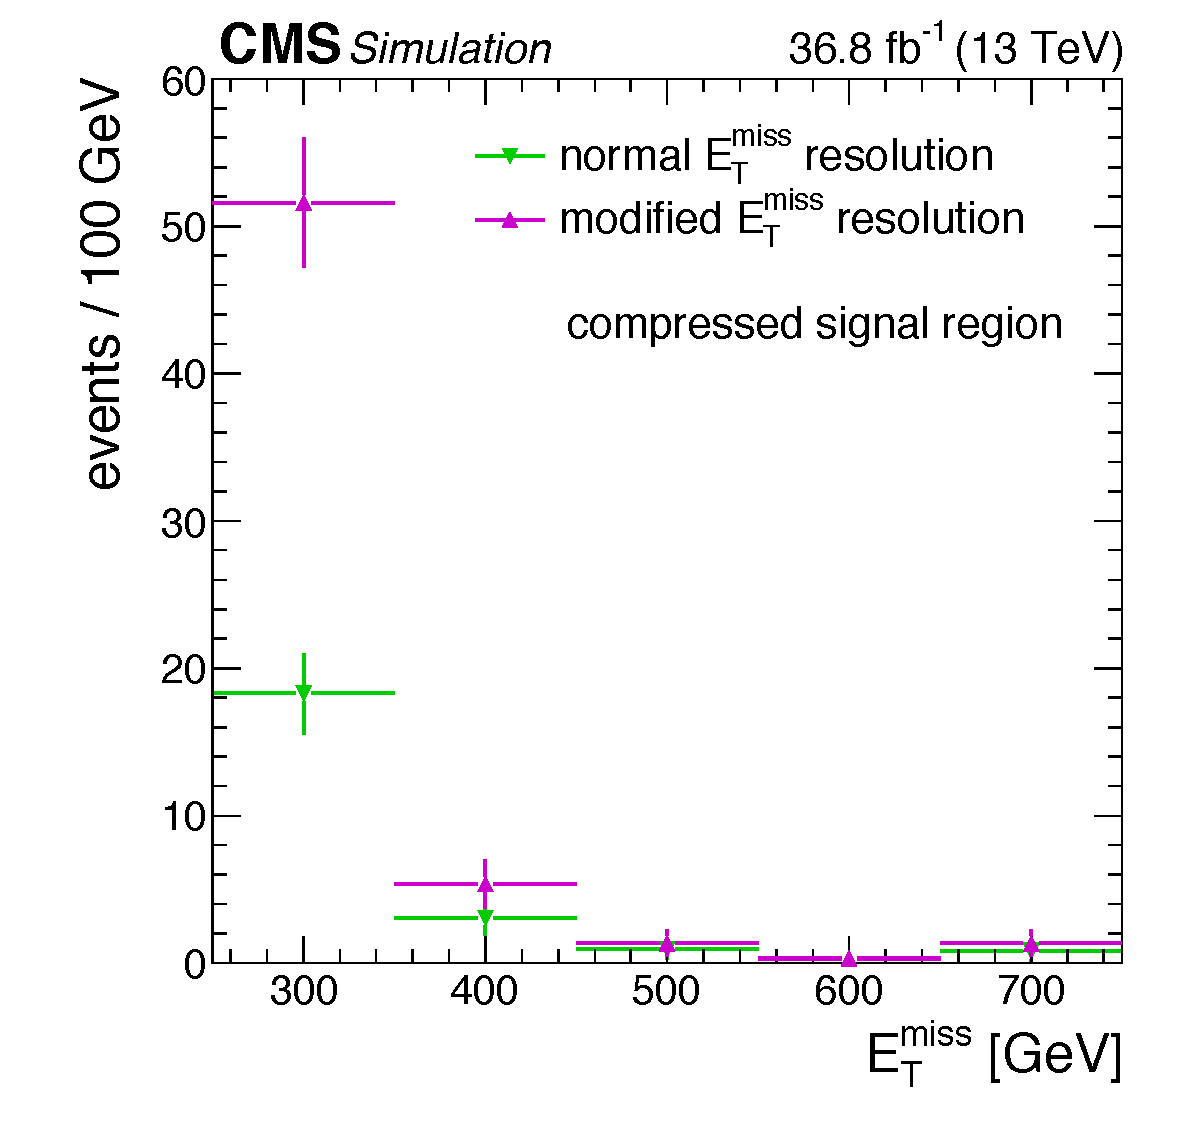
\includegraphics[width=0.45\textwidth]{figures/metres_1ltop_I.pdf}
\caption{$\met$ distributions in $\ttonelep$ Monte Carlo, with and
  without fluctuated $\met$ resolution. The plots are made
  in the C regions, the D regions, the combined E/F/G/H regions, and
  the I (corridor) regions, respectively. The A/B regions have an
  insignificant $\ttonelep$ component, so are not shown.}
\label{fig:stop:1ltop:metres}
\end{figure}

The final results of our single lepton from top background estimate
are presented in Table \ref{tab:stop:1ltop:results}.

% 1ltop background table. Numbers come from paper draft. Table
% structure I cobbled together from bits and pieces of other stuff.
\begin{table}[htbp]
\centering
\caption{Results of the single lepton from top background estimate,
  with 100\% uncertainty applied.}
\label{tab:stop:1ltop:results}
\begin{tabular}{|l|c|c|}
\hline
Region & $\met$ bin & SR Estimate\\
\hline
$<4$ jets,~$\tmod \ge10.0$,~$\mlb <175$ & $250<\met<350$ &  ---  \\
$<4$ jets,~$\tmod \ge10.0$,~$\mlb <175$ & $350<\met<450$ &  0.22$\pm$0.22 \\
$<4$ jets,~$\tmod \ge10.0$,~$\mlb <175$ & $450<\met<600$ &  0.13$\pm$0.13  \\
$<4$ jets,~$\tmod \ge10.0$,~$\mlb <175$ & $\met>600$     &  0.28$\pm$0.28 \\
\hline
$<4$ jets,~$\tmod \ge10.0$,~$\mlb \ge175$ & $250<\met<450$ &  --- \\
$<4$ jets,~$\tmod \ge10.0$,~$\mlb \ge175$ & $450<\met<600$ &  ---  \\
$<4$ jets,~$\tmod \ge10.0$,~$\mlb \ge175$ & $\met>600$     &  ---  \\
\hline
$\ge4$ jets,~$\tmod <0.0$,~$\mlb <175$ & $250<\met<350$ &  13.2$\pm$13.2  \\
$\ge4$ jets,~$\tmod <0.0$,~$\mlb <175$ & $350<\met<450$ &  2.3$\pm$2.3  \\
$\ge4$ jets,~$\tmod <0.0$,~$\mlb <175$ & $450<\met<550$ &  0.63$\pm$0.63  \\
$\ge4$ jets,~$\tmod <0.0$,~$\mlb <175$ & $550<\met<650$ &  0.09$\pm$0.09 \\
$\ge4$ jets,~$\tmod <0.0$,~$\mlb <175$ & $\met>650$     &  --- \\
\hline
$\ge4$ jets,~$\tmod <0.0$,~$\mlb \ge175$ & $250<\met<350$ &  3.1$\pm$3.1  \\
$\ge4$ jets,~$\tmod <0.0$,~$\mlb \ge175$ & $350<\met<450$ &  0.59$\pm$0.59  \\
$\ge4$ jets,~$\tmod <0.0$,~$\mlb \ge175$ & $450<\met<550$ &  0.37$\pm$0.37  \\
$\ge4$ jets,~$\tmod <0.0$,~$\mlb \ge175$ & $\met>550$     &  ---  \\
\hline
$\ge4$ jets,~$0.0< \tmod <10.0$,~$\mlb <175$ & $250<\met<350$ &  1.7$\pm$1.7  \\
$\ge4$ jets,~$0.0< \tmod <10.0$,~$\mlb <175$ & $350<\met<550$ &  0.48$\pm$0.48  \\
$\ge4$ jets,~$0.0< \tmod <10.0$,~$\mlb <175$ & $\met>550$     &  0.33$\pm$0.33  \\
\hline
$\ge4$ jets,~$0.0< \tmod <10.0$,~$\mlb \ge175$ & $250<\met<450$ &  0.30$\pm$0.30  \\
$\ge4$ jets,~$0.0< \tmod <10.0$,~$\mlb \ge175$ & $\met>450$     &  ---  \\
\hline
$\ge4$ jets,~$\tmod \ge10.0$,~$\mlb <175$ & $250<\met<350$ &  0.75$\pm$0.75  \\
$\ge4$ jets,~$\tmod \ge10.0$,~$\mlb <175$ & $350<\met<450$ &  0.69$\pm$0.69  \\
$\ge4$ jets,~$\tmod \ge10.0$,~$\mlb <175$ & $450<\met<600$ &  0.10$\pm$0.10 \\
$\ge4$ jets,~$\tmod \ge10.0$,~$\mlb <175$ & $\met>600$     &  0.65$\pm$0.65  \\
\hline
$\ge4$ jets,~$\tmod \ge10.0$,~$\mlb \ge175$ & $250<\met<450$ &  ---  \\
$\ge4$ jets,~$\tmod \ge10.0$,~$\mlb \ge175$ & $\met>450$     &  0.11$\pm$0.11 \\
\hline
Compressed search & $250<\met<350$ & 5.3$\pm$5.3 \\
Compressed search & $350<\met<450$ & 1.0$\pm$1.0 \\
Compressed search & $450<\met<550$ & 0.12$\pm$0.12 \\
Compressed search & $\met>550$     & 0.13$\pm$0.13 \\
\hline
\end{tabular}
\end{table}

\subsection{Rare Standard Model Processes}
\label{ssec:stop:rarebkg}

The final component to our backgrounds is that from
rare Standard Model processes. In practice, we define this background
component to contain any events containing a Z-boson that decays to
two neutrinos (effectively becoming invisible). The vast majority of
these events come from ttZ production where the Z decays to
neutrinos, especially in the $\geq$4-jet regions. The next largest
source is WZ production, which manifests primarily in the 2-to-3-jet
regions.

\subsubsection{Estimation Method}
\label{sssec:stop:rarebkg:estimation}

Although the rare background is a relatively small component, we still
attempt to estimate it using robust, data-driven methods. In contrast
to the methods used for the lost lepton and 1$\ell$W backgrounds, we
estimate the rare background using a technique more akin to that used
in the top asymmetry measurements, as described in Section
\ref{sec:afb:background}.

Our rare background estimate relies on the assumption that the relative
normalization between data and MC is the same in our signal regions as
in a three-lepton control region. So:
\begin{equation}
\label{eq:stop:rarebkg:rationm}
\frac{N_\text{rare}^\text{SR}}{M_\text{rare}^\text{SR}} =
\frac{N_\text{ttZ, WZ}^{CR3\ell}}{M_\text{ttZ, WZ}^{CR3\ell}}
\end{equation}
If we invert Equation \ref{eq:stop:rarebkg:rationm}, we can estimate
our rare background component using the Monte Carlo yield in our
signal region, times a normalization factor derived in the 3$\ell$
control region:
\begin{equation}
\label{eq:stop:rarebkg:estimation}
N_\text{rare}^\text{SR} = M_\text{rare}^\text{SR} \times
NF_\text{ttZ, WZ}^{CR 3\ell}
\end{equation}
The normalization factors are derived using a template fit, separately
for ttZ and WZ production, as shown in Figure
\ref{fig:stop:rarebkg:normalization}. For ttZ, the factor is $1.14 \pm
0.30$, and for WZ, it is $1.26 \pm 0.09$. The uncertainties
incorporate both statistical and systematic factors that influence the
template fit.

% Plots of ttZ and WZ normalization fits, taken from AN-16-386.
\begin{figure}[htb]
\centering
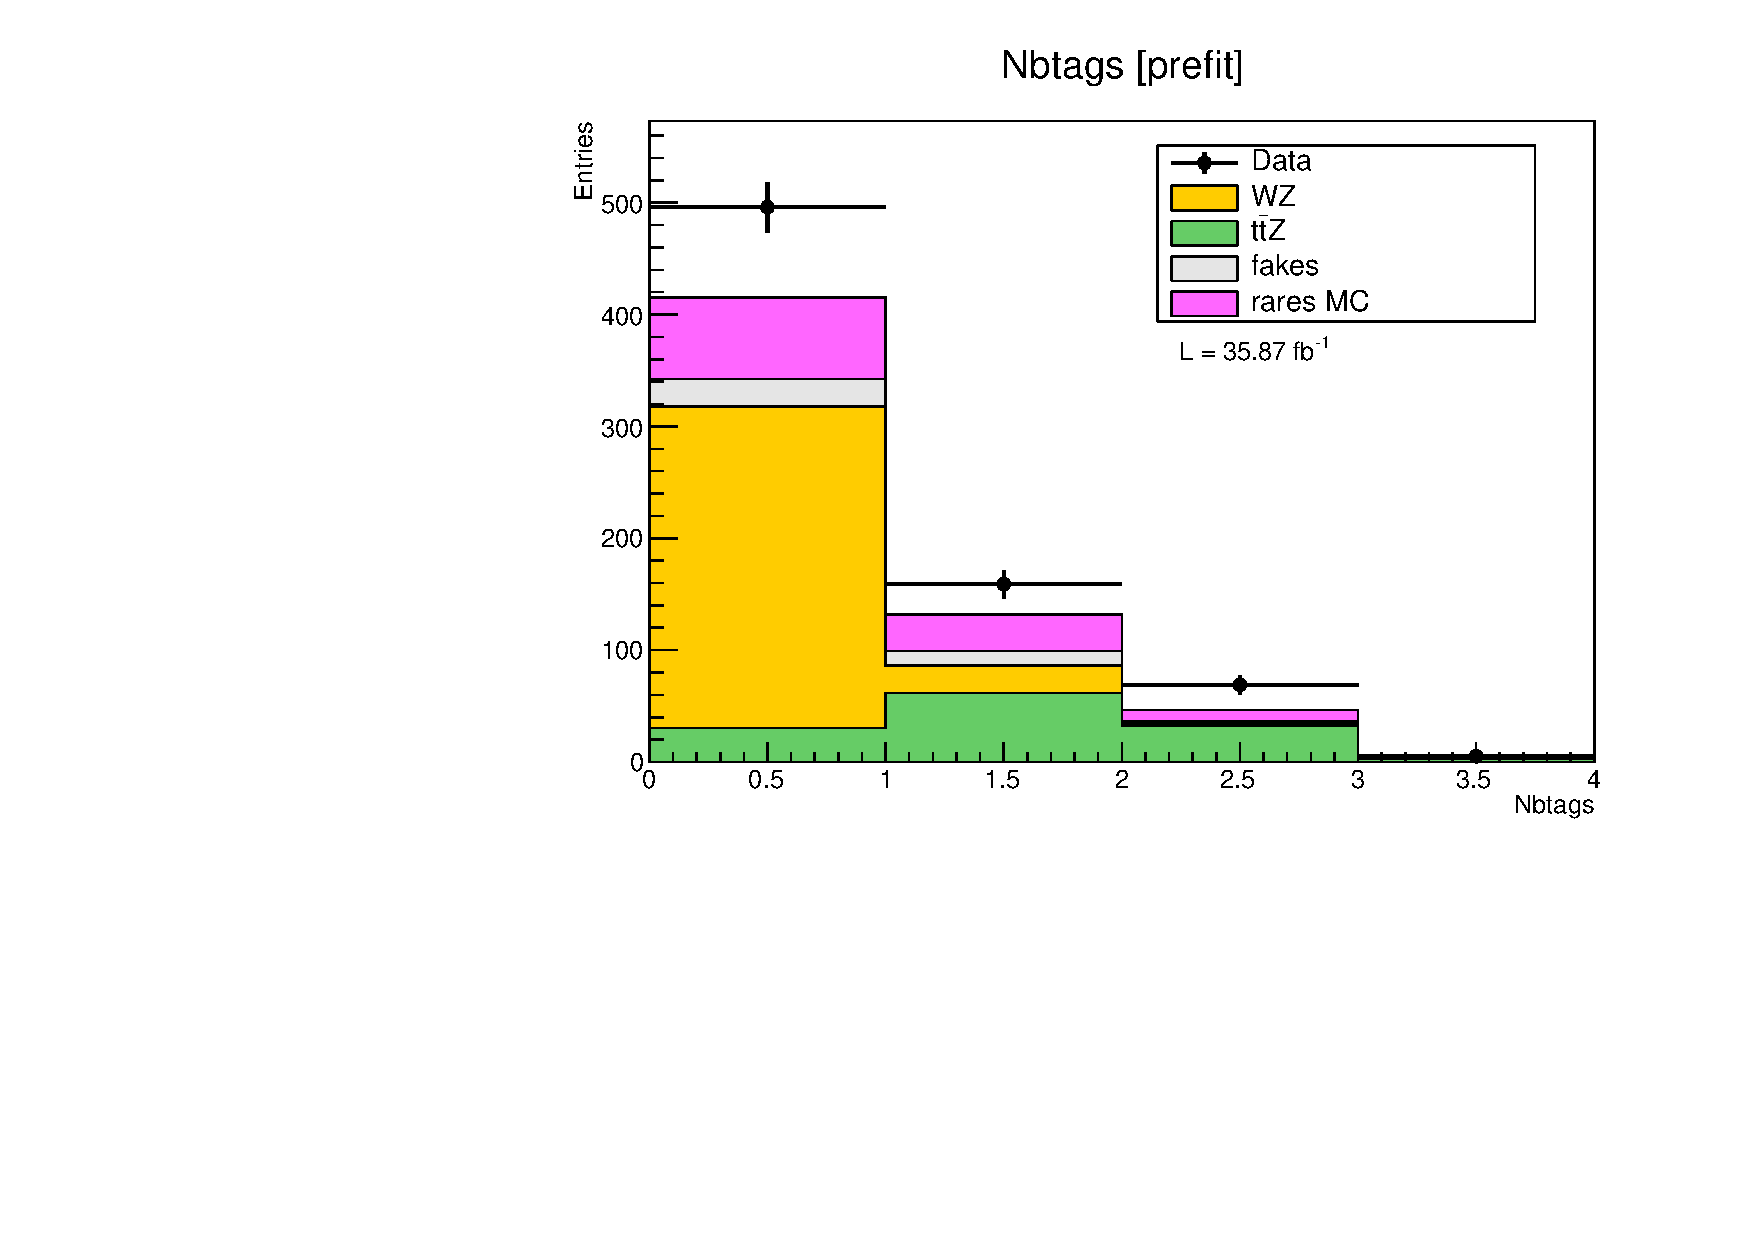
\includegraphics[width=0.45\textwidth]{figures/rarebkg_norm_prefit.pdf}
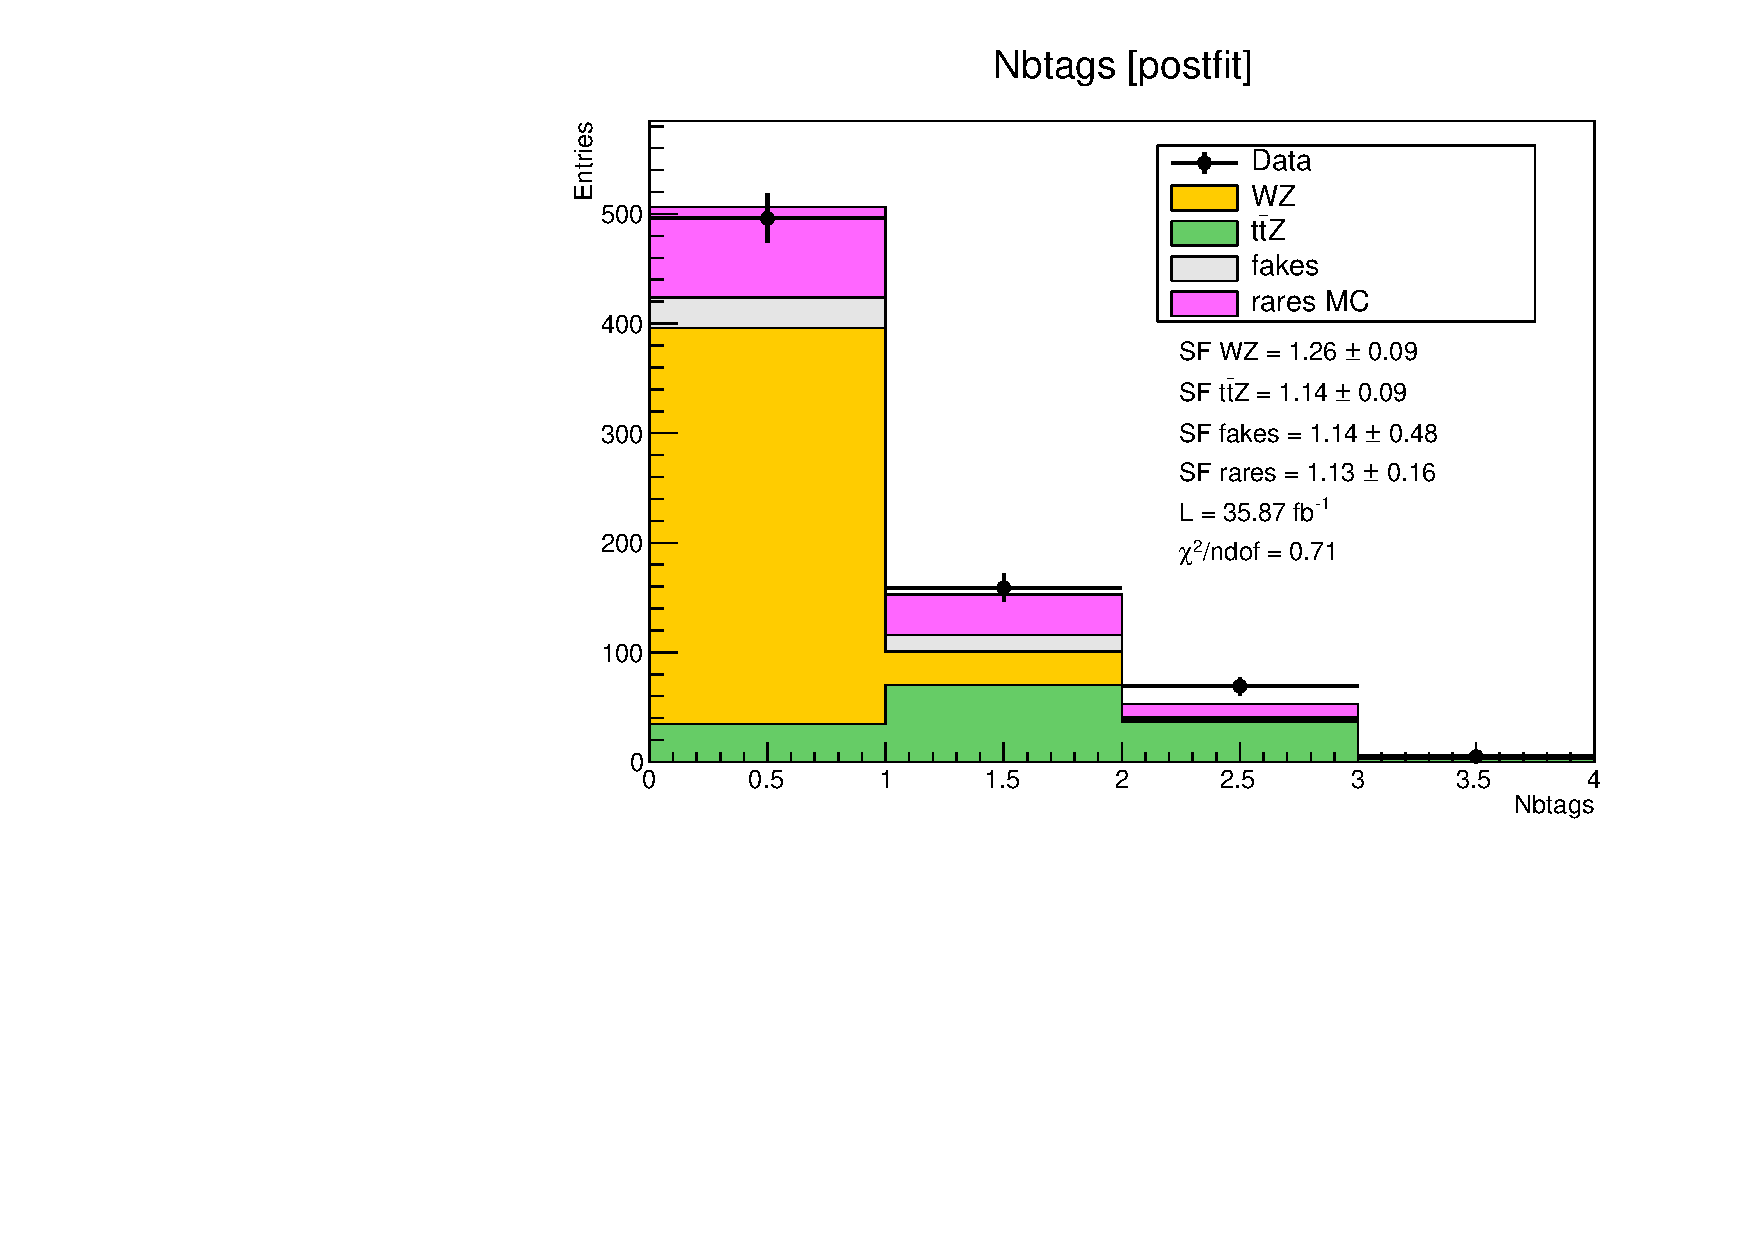
\includegraphics[width=0.45\textwidth]{figures/rarebkg_norm_postfit.pdf}
\caption{Distribution of number of b-jets in 3$\ell$ control region,
  before (left) and after (right) template fit, from 2016 same-sign dilepton search.}
\label{fig:stop:rarebkg:normalization}
\end{figure}

We do not derive these factors ourselves; rather, they are taken
from a CMS internal note documenting changes and improvements to the
2016 same-sign dilepton search. The same-sign analysis was described
in public documentation supporting ICHEP 2016 \cite{samesign}.
% AN-2016-386, follow up to PAS SUS-16-020

\subsubsection{Control Region Definition}
\label{sssec:stop:rarebkg:crdefinitions}

The control region used to select 3-lepton events for the same-sign
analysis is formed from the following criteria:
\begin{itemize}
\item Require three leptons ($e$ or $\mu$) passing tight ID
  criteria. The first two must have $p_T >$ 25 and 20 GeV,
  respectively, and the third must have $p_T >$ 10 GeV.
\item The third lepton must form an opposite-sign same-flavor pair
  with one of the first two leptons.
\item The invariant mass of the paired leptons must be within 15 GeV
  of the Z-boson mass (91.1876 GeV \cite{pdg}).
\item There must be at least two jets in the event.
\item The scalar sum of the $p_T$ of the jets, known as $H_T$, must
  be $>$ 80 GeV.
\item $\met >$ 30 GeV
\end{itemize}

\subsubsection{Systematic Uncertainties}
\label{sssec:stop:rarebkg:systematics}

Because the rare background is estimated differently from the other
backgrounds, we assess our systematic uncertainties in two different
ways. The standard experimental systematics are evaluated exactly as
they were for the lost lepton and 1$\ell$W backgrounds, except where
explicitly stated otherwise. The experimental uncertainties include:
\begin{itemize}
\item Monte Carlo statistics
\item b-tagging efficiencies (HF and LF)
\item Lepton ID and isolation efficiencies
\item JES
\item ISR $n_\text{jets}$ reweighting
\item \textbf{Pileup reweighting:} this systematic is highly sensitive to the
  low MC statistics of this background. To avoid large fluctuations,
  we evaluate the uncertainty across all signal regions summed
  together, and see that a conservative 3\% systematic will cover all
  realistic cases.
\end{itemize}

When evaluating the theory uncertainties, we only consider the effects
they have on the shape of the background. We keep the normalization
fixed to the values derived from the control region. And because the
theory uncertainties are highly sensitive to our limited statistics,
we merge several of the nominal regions together by removing the
binning in $\mlb$ and $\tmod$. In effect, this leaves us
with fewer regions, binned only in $N_\text{jets}$ and $\met$. The
corridor regions are not merged in any way. This merging is justified
by studies showing that variations in the shapes of $\mlb$ and
$\tmod$ are small compared to uncertainties arising from the
$\met$ distribution. The theory uncertainties evaluated in this manner
are:
\begin{itemize}
\item $Q^2$
\item PDF
\item $\alpha_S$
\end{itemize}

The values of the systematic uncertainties are presented in Table
\ref{tab:stop:rarebkg:systematics}

% Table of systematics adapted from AN-16-463.
\begin{sidewaystable}
\centering
\footnotesize
\caption{Summary of systematic uncertainties on the rare standard
  model processes background estimate.}
\label{tab:stop:rarebkg:systematics}
\begin{tabular}{|l|ccccccccccc|c|}
\hline
Region & MC stat.   &   Lep. ID/Iso   &   b-tag (LF) &   b-tag (HF)  &   PU &   PDF &   $\alpha_S$ &   $Q^2$ &   ISR njets  & JES &   Norm.  & Total \\
\hline
 A $250<\met<350$ & 11.88\% & 0.31\%  & 1.58\%  & 1.23\%  & 3.00\%  & 0.23\%  & 0.86\%  & 3.86\%  & 7.12\%  & 2.55\%  & 20.70\% & 25.60\% \\
 A $350<\met<450$ & 25.04\% & 0.35\%  & 3.63\%  & 0.77\%  & 3.00\%  & 3.33\%  & 0.61\%  & 1.31\%  & 9.09\%  & 0.37\%  & 24.38\% & 36.61\% \\
 A $450<\met<600$ & 23.87\% & 0.37\%  & 1.34\%  & 1.34\%  & 3.00\%  & 0.45\%  & 0.39\%  & 2.47\%  & 7.02\%  & 0.46\%  & 20.77\% & 32.71\% \\
 A $\met>600$     & 51.43\% & 0.41\%  & 2.87\%  & 1.74\%  & 3.00\%  & 8.04\%  & 0.36\%  & 2.37\%  & 5.13\%  & 10.54\% & 16.77\% & 56.17\% \\
 B $250<\met<450$ & 29.98\% & 0.50\%  & 1.67\%  & 1.23\%  & 3.00\%  & 1.17\%  & 0.76\%  & 2.86\%  & 3.97\%  & 1.01\%  & 14.74\% & 34.01\% \\
 B $450<\met<600$ & 86.04\% & 0.77\%  & 5.28\%  & 1.26\%  & 3.00\%  & 0.45\%  & 0.40\%  & 2.47\%  & 4.00\%  & 32.62\% & 15.46\% & 93.63\% \\
 B $\met>600$     & 228.31\%& 2.65\%  & 19.40\% & 1.64\%  & 3.00\%  & 8.03\%  & 0.36\%  & 2.37\%  & 8.12\%  & 44.04\% & 22.72\% & 234.76\%\\
 C $250<\met<350$ & 4.56\%  & 0.45\%  & 0.06\%  & 0.68\%  & 3.00\%  & 0.81\%  & 0.60\%  & 1.77\%  & 0.40\%  & 4.78\%  & 26.18\% & 27.26\% \\
 C $350<\met<450$ & 10.85\% & 0.35\%  & 0.48\%  & 0.66\%  & 3.00\%  & 2.01\%  & 1.23\%  & 5.00\%  & 0.99\%  & 6.85\%  & 23.73\% & 27.73\% \\
 C $450<\met<550$ & 20.70\% & 0.31\%  & 4.53\%  & 0.26\%  & 3.00\%  & 1.89\%  & 1.34\%  & 4.86\%  & 2.03\%  & 4.52\%  & 18.54\% & 29.25\% \\
 C $550<\met<650$ & 9.20\%  & 0.38\%  & 0.77\%  & 0.38\%  & 3.00\%  & 4.90\%  & 1.86\%  & 3.67\%  & 3.67\%  & 2.14\%  & 26.32\% & 29.09\% \\
 C $\met>650$     & 12.73\% & 0.45\%  & 0.20\%  & 0.40\%  & 3.00\%  & 8.11\%  & 3.08\%  & 4.23\%  & 4.92\%  & 5.74\%  & 26.32\% & 31.85\% \\
 D $250<\met<350$ & 19.82\% & 0.31\%  & 0.72\%  & 0.41\%  & 3.00\%  & 0.81\%  & 0.60\%  & 1.76\%  & 0.82\%  & 9.76\%  & 20.24\% & 30.20\% \\
 D $350<\met<450$ & 27.58\% & 0.32\%  & 1.82\%  & 1.08\%  & 3.00\%  & 2.02\%  & 1.23\%  & 4.99\%  & 1.63\%  & 10.79\% & 17.33\% & 34.98\% \\
 D $450<\met<550$ & 47.40\% & 0.33\%  & 4.96\%  & 0.22\%  & 3.00\%  & 1.88\%  & 1.33\%  & 4.85\%  & 2.24\%  & 17.87\% & 17.31\% & 54.17\% \\
 D $\met>550$     & 18.94\% & 0.44\%  & 0.06\%  & 0.83\%  & 3.00\%  & 7.53\%  & 2.44\%  & 2.55\%  & 7.31\%  & 7.15\%  & 26.32\% & 35.14\% \\
 E $250<\met<350$ & 5.55\%  & 0.42\%  & 0.65\%  & 0.74\%  & 3.00\%  & 0.81\%  & 0.60\%  & 1.77\%  & 2.52\%  & 3.80\%  & 25.40\% & 26.66\% \\
 E $350<\met<550$ & 10.40\% & 0.40\%  & 0.01\%  & 0.83\%  & 3.00\%  & 1.97\%  & 1.26\%  & 4.96\%  & 0.66\%  & 7.23\%  & 23.72\% & 27.63\% \\
 E $\met>550$     & 87.72\% & 0.77\%  & 7.05\%  & 0.02\%  & 3.00\%  & 7.55\%  & 2.47\%  & 2.51\%  & 2.26\%  & 1.66\%  & 24.61\% & 91.86\% \\
 F $250<\met<450$ & 16.02\% & 0.42\%  & 0.06\%  & 0.31\%  & 3.00\%  & 1.16\%  & 0.78\%  & 2.70\%  & 2.10\%  & 4.41\%  & 24.07\% & 29.63\% \\
 F $\met>450$     & 12.82\% & 0.47\%  & 0.40\%  & 0.57\%  & 3.00\%  & 3.72\%  & 1.70\%  & 3.91\%  & 2.22\%  & 3.37\%  & 26.33\% & 30.26\% \\
 G $250<\met<350$ & 5.75\%  & 0.39\%  & 0.01\%  & 1.71\%  & 3.00\%  & 0.81\%  & 0.60\%  & 1.77\%  & 2.09\%  & 3.44\%  & 25.42\% & 26.68\% \\
 G $350<\met<450$ & 7.06\%  & 0.43\%  & 0.05\%  & 1.35\%  & 3.00\%  & 2.01\%  & 1.23\%  & 5.00\%  & 1.79\%  & 9.62\%  & 25.14\% & 28.63\% \\
 G $450<\met<600$ & 9.01\%  & 0.37\%  & 0.19\%  & 1.27\%  & 3.00\%  & 2.63\%  & 1.54\%  & 4.72\%  & 0.51\%  & 5.15\%  & 24.77\% & 27.64\% \\
 G $\met>600$     & 7.00\%  & 0.47\%  & 0.19\%  & 1.01\%  & 3.00\%  & 8.01\%  & 2.34\%  & 1.74\%  & 0.68\%  & 15.62\% & 26.32\% & 32.70\% \\
 H $250<\met<450$ & 9.94\%  & 0.49\%  & 0.05\%  & 0.07\%  & 3.00\%  & 1.17\%  & 0.79\%  & 2.72\%  & 2.06\%  & 4.60\%  & 26.32\% & 28.91\% \\
 H $\met>450$     & 34.01\% & 0.43\%  & 0.04\%  & 0.88\%  & 3.00\%  & 3.71\%  & 1.70\%  & 3.91\%  & 0.93\%  & 2.41\%  & 19.94\% & 40.03\% \\
 I $250<\met<350$ & 9.76\%  & 0.38\%  & 0.78\%  & 0.47\%  & 3.00\%  & 0.21\%  & 0.32\%  & 3.91\%  & 4.30\%  & 5.32\%  & 23.38\% & 26.72\% \\
 I $350<\met<450$ & 17.91\% & 0.35\%  & 0.76\%  & 0.60\%  & 3.00\%  & 1.99\%  & 1.41\%  & 5.88\%  & 4.56\%  & 6.05\%  & 22.78\% & 30.79\% \\
 I $450<\met<550$ & 25.04\% & 0.51\%  & 4.83\%  & 0.35\%  & 3.00\%  & 1.89\%  & 1.62\%  & 4.90\%  & 5.38\%  & 4.89\%  & 21.64\% & 34.80\% \\
 I $\met>550$     & 29.62\% & 0.40\%  & 0.22\%  & 0.68\%  & 3.00\%  & 1.82\%  & 1.55\%  & 7.48\%  & 4.76\%  & 6.34\%  & 20.76\% & 37.98\% \\
\hline
\end{tabular}
\end{sidewaystable}

\subsubsection{Results}
\label{sssec:stop:rarebkg:results}

The results of the rare standard model background estimation procedure
are presented in Table \ref{tab:stop:rarebkg:results}.

% Results table taken from AN-16-463.
\begin{table}[htbp]
\centering
\caption{Summary of the rare standard model background
  estimate.}
\label{tab:stop:rarebkg:results}
\begin{tabular}{|l|cc|c|}
\hline
Region & ttZ & WZ & Total  \\
\hline
 A $250<\met<350$ & 3.33 $\pm$ 0.96   & 1.38 $\pm$ 0.58   & 4.71 $\pm$ 1.21   \\
 A $350<\met<450$ & 1.85 $\pm$ 0.53   & 0.21 $\pm$ 0.53   & 2.05 $\pm$ 0.75   \\
 A $450<\met<600$ & 1.15 $\pm$ 0.33   & 0.47 $\pm$ 0.39   & 1.62 $\pm$ 0.53   \\
 A $\met>600$ & 0.36 $\pm$ 0.11   & 0.36 $\pm$ 0.41   & 0.71 $\pm$ 0.40   \\
 B $250<\met<450$ & 0.61 $\pm$ 0.18   & 0.93 $\pm$ 0.47   & 1.54 $\pm$ 0.52   \\
 B $450<\met<600$ & 0.15 $\pm$ 0.05   & 0.20 $\pm$ 0.34   & 0.35 $\pm$ 0.33   \\
 B $\met>600$ & 0.09 $\pm$ 0.03   & 0.02 $\pm$ 0.26   & 0.11 $\pm$ 0.26   \\
 C $250<\met<350$ & 14.28 $\pm$ 3.84  & 0.10 $\pm$ 0.62   & 14.38 $\pm$ 3.92  \\
 C $350<\met<450$ & 3.83 $\pm$ 1.06   & 0.60 $\pm$ 0.48   & 4.43 $\pm$ 1.23   \\
 C $450<\met<550$ & 1.06 $\pm$ 0.31   & 0.73 $\pm$ 0.39   & 1.79 $\pm$ 0.52   \\
 C $550<\met<650$ & 0.40 $\pm$ 0.12   & 0.00 $\pm$ 0.00   & 0.40 $\pm$ 0.12   \\
 C $\met>650$ & 0.20 $\pm$ 0.06   & 0.00 $\pm$ 0.00   & 0.20 $\pm$ 0.06   \\
 D $250<\met<350$ & 2.06 $\pm$ 0.56   & 0.95 $\pm$ 0.63   & 3.01 $\pm$ 0.91   \\
 D $350<\met<450$ & 0.62 $\pm$ 0.18   & 0.55 $\pm$ 0.40   & 1.18 $\pm$ 0.41   \\
 D $450<\met<550$ & 0.24 $\pm$ 0.07   & 0.21 $\pm$ 0.22   & 0.45 $\pm$ 0.24   \\
 D $\met>550$ & 0.09 $\pm$ 0.03   & 0.00 $\pm$ 0.00   & 0.09 $\pm$ 0.03   \\
 E $250<\met<350$ & 7.88 $\pm$ 2.14   & 0.40 $\pm$ 0.44   & 8.27 $\pm$ 2.21   \\
 E $350<\met<550$ & 3.34 $\pm$ 0.94   & 0.52 $\pm$ 0.39   & 3.87 $\pm$ 1.07   \\
 E $\met>550$ & 0.26 $\pm$ 0.08   & 0.03 $\pm$ 0.25   & 0.29 $\pm$ 0.26   \\
 F $250<\met<450$ & 0.98 $\pm$ 0.27   & 0.13 $\pm$ 0.17   & 1.11 $\pm$ 0.33   \\
 F $\met>450$ & 0.21 $\pm$ 0.06   & 0.00 $\pm$ 0.00   & 0.21 $\pm$ 0.06   \\
 G $250<\met<350$ & 2.89 $\pm$ 0.78   & 0.14 $\pm$ 0.15   & 3.03 $\pm$ 0.81   \\
 G $350<\met<450$ & 2.51 $\pm$ 0.71   & 0.16 $\pm$ 0.18   & 2.67 $\pm$ 0.77   \\
 G $450<\met<600$ & 1.80 $\pm$ 0.50   & 0.16 $\pm$ 0.16   & 1.96 $\pm$ 0.54   \\
 G $\met>600$ & 0.70 $\pm$ 0.20   & 0.00 $\pm$ 0.00   & 0.70 $\pm$ 0.23   \\
 H $250<\met<450$ & 0.37 $\pm$ 0.11   & 0.00 $\pm$ 0.00   & 0.37 $\pm$ 0.11   \\
 H $\met>450$ & 0.33 $\pm$ 0.10   & 0.16 $\pm$ 0.17   & 0.49 $\pm$ 0.20   \\
 I $250<\met<350$ & 3.66 $\pm$ 1.01   & 0.66 $\pm$ 0.43   & 4.33 $\pm$ 1.16   \\
 I $350<\met<450$ & 1.57 $\pm$ 0.45   & 0.35 $\pm$ 0.34   & 1.93 $\pm$ 0.59   \\
 I $450<\met<550$ & 0.58 $\pm$ 0.17   & 0.19 $\pm$ 0.20   & 0.77 $\pm$ 0.27   \\
 I $\met>550$ & 0.41 $\pm$ 0.13   & 0.17 $\pm$ 0.17   & 0.58 $\pm$ 0.22   \\
\hline
\end{tabular}
\end{table}

\section{Results}
\label{sec:stop:results}

The results of the four background estimation procedures, as well as
the yields of data in our signal regions, are presented in Table
\ref{tab:stop:results}. The same numbers are presented graphically in
Figure \ref{fig:stop:results}.

% Results table, adapted from AN-16-463.
\begin{table}[htbp]
\footnotesize
\centering
\caption{Estimated background yields and measured data yields in our
  signal regions, based on the full 35.9 fb\textsuperscript{-1} of
  2016 data.}
\label{tab:stop:results}
\scalebox{0.95}{
\begin{tabular}{|r|r|r|r|c|c|c|c|c|c|}
\hline
 \multirow{2}{*}{$N_\mathrm{J}$} & \multirow{2}{*}{$\tmod$} & $M_\mathrm{\ell b}$ & $E_\mathrm{T}^\mathrm{miss}$ & Lost  & \multirow{2}{*}{1$\ell$ (top)} & 1$\ell$ (not & \multirow{2}{*}{$Z\rightarrow\nu\bar{\nu}$} & Total & \multirow{2}{*}{Data} \\
  &  &  [GeV] &  [GeV] &  lepton &  &  top) &  & background &  \\
\hline
$\leq3$ &    $>10$ & $\leq175$ & $250-350$ & 53.9$\pm$6.2 & --- & 7.2$\pm$2.5 & 4.7$\pm$1.2 & 65.8$\pm$6.8 & 72 \\
$\leq3$ &    $>10$ & $\leq175$ & $350-450$ & 14.2$\pm$2.4 & 0.22$\pm$0.22 & 4.1$\pm$1.4 & 2.1$\pm$0.8 & 20.5$\pm$2.9 & 24 \\
$\leq3$ &    $>10$ & $\leq175$ & $450-600$ & 2.9$\pm$0.9 & 0.13$\pm$0.13 & 1.7$\pm$0.7 & 1.6$\pm$0.5 & 6.4$\pm$1.3 & 6 \\
$\leq3$ &    $>10$ & $\leq175$ &    $>600$ & 0.61$\pm$0.49 & 0.28$\pm$0.28 & 0.78$\pm$0.34 & 0.71$\pm$0.40 & 2.4$\pm$0.8 & 2 \\
\hline
$\leq3$ &    $>10$ &     $>175$ & $250-450$ & 1.7$\pm$0.8 & --- & 5.6$\pm$2.2 & 1.5$\pm$0.5 & 8.9$\pm$2.4 & 6 \\
$\leq3$ &    $>10$ &     $>175$ & $450-600$ & 0.02$\pm$0.01 & --- & 1.6$\pm$0.6 & 0.35$\pm$0.33 & 1.9$\pm$0.7 & 3 \\
$\leq3$ &    $>10$ &     $>175$ &    $>600$ & 0.01$\pm$0.01 & --- & 0.87$\pm$0.39 & 0.11$\pm$0.26 & 0.99$\pm$0.47 & 2 \\
\hline
$\geq4$ & $\leq0$ & $\leq175$ & $250-350$ & 346$\pm$30 & 13.2$\pm$13.2 & 9.7$\pm$8.6 & 14.4$\pm$3.9 & 383$\pm$34 & 343 \\
$\geq4$ & $\leq0$ & $\leq175$ & $350-450$ & 66.3$\pm$7.9 & 2.3$\pm$2.3 & 2.5$\pm$1.7 & 4.4$\pm$1.2 & 75.5$\pm$8.5 & 68 \\
$\geq4$ & $\leq0$ & $\leq175$ & $450-550$ & 12.1$\pm$2.8 & 0.63$\pm$0.63 & 0.47$\pm$0.46 & 1.8$\pm$0.5 & 15.0$\pm$2.9 & 13 \\
$\geq4$ & $\leq0$ & $\leq175$ & $550-650$ & 3.4$\pm$1.5 & 0.09$\pm$0.09 & 0.26$\pm$0.20 & 0.40$\pm$0.12 & 4.1$\pm$1.5 & 6 \\
$\geq4$ & $\leq0$ & $\leq175$ &    $>650$ & 5.9$\pm$2.8 & --- & 0.43$\pm$0.38 & 0.20$\pm$0.06 & 6.6$\pm$2.9 & 2 \\
\hline
$\geq4$ & $\leq0$ &     $>175$ & $250-350$ & 26.0$\pm$4.3 & 3.1$\pm$3.1 & 7.5$\pm$3.0 & 3.0$\pm$0.9 & 39.7$\pm$6.2 & 38 \\
$\geq4$ & $\leq0$ &     $>175$ & $350-450$ & 10.4$\pm$2.6 & 0.59$\pm$0.59 & 1.6$\pm$0.7 & 1.2$\pm$0.4 & 13.7$\pm$2.8 & 8 \\
$\geq4$ & $\leq0$ &     $>175$ & $450-550$ & 1.7$\pm$0.9 & 0.37$\pm$0.37 & 0.56$\pm$0.32 & 0.45$\pm$0.24 & 3.1$\pm$1.1 & 2 \\
$\geq4$ & $\leq0$ &     $>175$ &    $>550$ & 1.1$\pm$0.8 & --- & 1.0$\pm$0.6 & 0.09$\pm$0.03 & 2.2$\pm$1.0 & 1 \\
\hline
$\geq4$ &   $0-10$ & $\leq175$ & $250-350$ & 43.0$\pm$5.9 & 1.7$\pm$1.7 & 5.7$\pm$3.0 & 8.3$\pm$2.2 & 58.7$\pm$7.2 & 65 \\
$\geq4$ &   $0-10$ & $\leq175$ & $350-550$ & 9.1$\pm$2.0 & 0.48$\pm$0.48 & 1.2$\pm$0.5 & 3.9$\pm$1.1 & 14.7$\pm$2.4 & 23 \\
$\geq4$ &   $0-10$ & $\leq175$ &    $>550$ & 0.57$\pm$0.28 & 0.33$\pm$0.33 & 0.26$\pm$0.24 & 0.29$\pm$0.26 & 1.5$\pm$0.6 & 1 \\
\hline
$\geq4$ &   $0-10$ &     $>175$ & $250-450$ & 4.4$\pm$1.4 & 0.30$\pm$0.30 & 3.1$\pm$1.3 & 1.1$\pm$0.3 & 8.9$\pm$1.9 & 9 \\
$\geq4$ &   $0-10$ &     $>175$ &    $>450$ & 0.10$\pm$0.17 & --- & 0.24$\pm$0.16 & 0.21$\pm$0.06 & 0.56$\pm$0.24 & 0 \\
\hline
$\geq4$ &    $>10$ & $\leq175$ & $250-350$ & 9.5$\pm$2.3 & 0.75$\pm$0.75 & 1.1$\pm$0.9 & 3.0$\pm$0.8 & 14.3$\pm$2.7 & 12 \\
$\geq4$ &    $>10$ & $\leq175$ & $350-450$ & 5.9$\pm$1.8 & 0.69$\pm$0.69 & 0.71$\pm$0.51 & 2.7$\pm$0.8 & 10.0$\pm$2.1 & 9 \\
$\geq4$ &    $>10$ & $\leq175$ & $450-600$ & 3.8$\pm$1.3 & 0.10$\pm$0.10 & 0.43$\pm$0.32 & 2.0$\pm$0.5 & 6.3$\pm$1.5 & 3 \\
$\geq4$ &    $>10$ & $\leq175$ &    $>600$ & 0.75$\pm$0.61 & 0.65$\pm$0.65 & 0.34$\pm$0.38 & 0.70$\pm$0.23 & 2.4$\pm$1.0 & 0 \\
\hline
$\geq4$ &    $>10$ &     $>175$ & $250-450$ & 0.54$\pm$0.32 & --- & 1.0$\pm$0.6 & 0.37$\pm$0.11 & 1.9$\pm$0.7 & 0 \\
$\geq4$ &    $>10$ &     $>175$ &    $>450$ & 0.24$\pm$0.17 & 0.11$\pm$0.11 & 0.46$\pm$0.26 & 0.49$\pm$0.20 & 1.3$\pm$0.4 & 2 \\
\hline
\multicolumn{3}{|l|}{Corridor region} & $250-350$ & 67.5$\pm$8.9 & 5.3$\pm$5.3 & 5.0$\pm$1.8 & 4.3$\pm$1.2 & 82.2$\pm$10.6 & 72 \\
\multicolumn{3}{|l|}{Corridor region} & $350-450$ & 15.1$\pm$3.5 & 1.0$\pm$1.0 & 0.84$\pm$0.33 & 1.9$\pm$0.6 & 18.9$\pm$3.7 & 30 \\
\multicolumn{3}{|l|}{Corridor region} & $450-550$ & 2.4$\pm$1.3 & 0.12$\pm$0.12 & 0.42$\pm$0.24 & 0.77$\pm$0.27 & 3.7$\pm$1.4 & 2 \\
\multicolumn{3}{|l|}{Corridor region} &    $>550$ & 3.9$\pm$2.0 & 0.13$\pm$0.13 & 0.24$\pm$0.17 & 0.58$\pm$0.22 & 4.8$\pm$2.0 & 2 \\
\hline
\end{tabular}}
\end{table}

% Plot of final results, taken from SUS-16-051 paper draft.
\begin{figure}[htb]
\centering
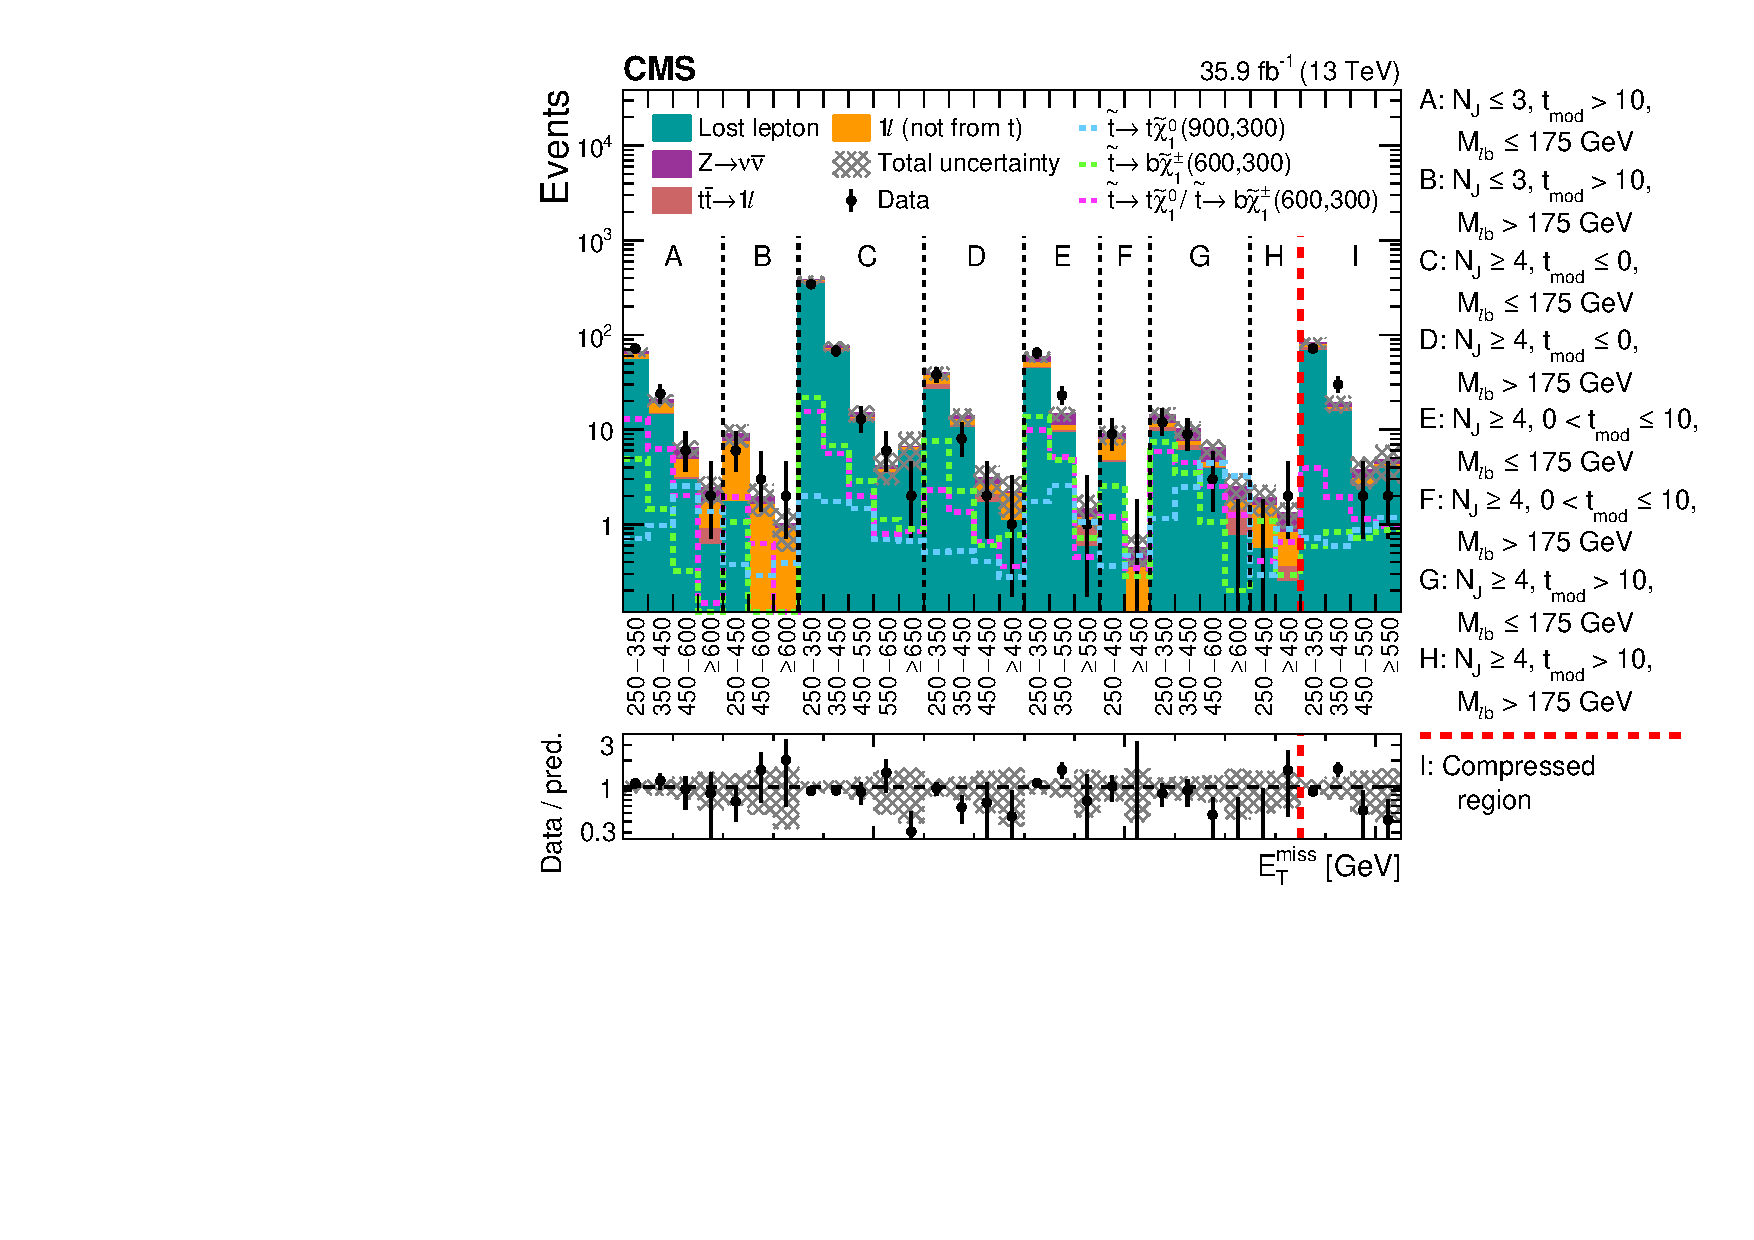
\includegraphics[width=0.99\textwidth]{figures/ResultPlot_Moriond2017.pdf}
\caption{Estimated background yields, measured data yields, and
  selected signal predictions in our signal regions, based on the full
  35.9 fb\textsuperscript{-1} of 2016 data. Hatched bands show the
  combined statistical and systematic uncertainties.}
\label{fig:stop:results}
\end{figure}

\section{Interpretation}
\label{sec:stop:interp}

\subsection{Signal Estimate}
\label{ssec:stop:signal}

With the final tally of data and estimated backgrounds in, we must
interpret those counts in terms of our SUSY signal models. As
described in Table \ref{tab:stop:mcsamples}, our signal predictions
are drawn from several Monte Carlo samples, produced using FastSim.

During the course of routine data analysis, CMS scientists discovered
certain anomalous events in the samples produced using FastSim. To
prevent this anomaly from impacting our analysis, we filter out all
simulated signal events that contain a reconstructed jet with the
following attributes:
\begin{itemize}
\item Not matched to a generated jet within $\Delta R <$ 0.3, and
\item Charged hadron fraction (CHF) $<$ 0.1
\end{itemize}

\subsubsection{Systematic Uncertainties}
\label{sssec:stop:signal:systematics}

Because our signal predictions are drawn from Monte Carlo simulations,
we must assess many of the same systematic uncertainties for signal as
we did for our background estimates. Although FastSim and FullSim have
separate correction factors for a number of uncertainties, the method
used to apply those corrections is generally the same as has been
described for the background estimates.

For signal samples, we compute an uncertainty on the lepton veto
efficiency separately. All our signal models have an efficiency of
about 94\% to accept true single-lepton events, with the 6\%
inefficiency due to fake leptons. We assess a 50\% uncertainty on the
efficiency of identifying these fake leptons, effectively giving a 3\%
systematic for lepton veto efficiency.

In addition, we must correct for the different modeling of $\met$ resolution % Note that this is different from the MET resolution SF
in FastSim. To make such a correction, whenever $\met$ enters our
measurements, we take the average of the reconstructed and generated
$\met$ values. Effectively:
\begin{equation}
\met \text{(signal)} = \frac{1}{2} \left( \met \text{(reconstructed)} + \met
  \text{(generated)} \right)
\end{equation}
To evaluate the uncertainty on this $\met$ correction, we vary the
$\met$ by half the difference between the reconstructed and generated
$\met$ values. % Is this the same as varying it between recomet and genmet?

A condensed summary of the uncertainties on the signal estimate is
presented in Table \ref{tab:stop:signal:systematics}.

% Signal systematics table, adapted from AN-16-463
\begin{table}[htbp]
\centering
\caption{Summary of systematic uncertainties on signal
  yields. Uncertainties are given as typical values for an individual
  signal region. Low $\Delta M$ refers to the compressed
  regions. Table also indicates which uncertainties are treated as
  correlated between regions.}
\label{tab:stop:signal:systematics}
\begin{tabular}{lccc}
\hline\hline
Systematic & \multicolumn{2}{c}{Typical size} & Correlated \\
 & low $\Delta M$ & high $\Delta M$ & \\
\hline
Monte Carlo statistics & 7--15\% & 5--25\% & ---  \\
Luminosity & 2.5\% & 2.5\% & $\checkmark$  \\
Trigger & 2--4\% & 2--4\% & $\checkmark$  \\
Pile-Up & 5--10\% & 5-10\% & ---  \\
ISR & 15\% & 1--8\% & $\checkmark$ \\
Jet energy scale & 1-20\% & 1-12\% & $\checkmark$ \\
$Q^2$ & 2--4\% & 2-4\% & $\checkmark$ \\
b-tagging & 1--2\% & 1--7\% & $\checkmark$ \\
Lepton ID/ISO & 1\% & 1--2\% & $\checkmark$ \\
Lepton veto efficiency & 3\% & 3\% & --- \\
$\met$ modeling & 2--7\% & 1--10\% & --- \\
\hline\hline
\end{tabular}
\end{table}

\subsubsection{Signal Contamination}
\label{sssec:stop:signal:contamination}

Because our dilepton and 0-btag control regions are so similar to our
signal regions, with only single cuts inverted, a number of signal
events are reconstructed in those control regions instead of in the
signal regions. This is known as \emph{signal contamination}. This
contamination could cause our background estimates to be
artificially high, thus preventing us from noticing any excess of SUSY
events in our signal regions. To account for this effect, we measure
the number of signal events in our lost lepton and 0-btag control
regions, and propagate those numbers through our estimation procedure,
to figure out how the contamination would raise our background
predictions. We then subtract those numbers from the signal yields
predicted in the signal regions. This has the effect of reducing our
sensitivity to SUSY signals in a way that approximates the effect of
actual signal contamination.

Signal contamination in the lost lepton CRs results in a signal yield
correction of 5-10\% in the top and W corridor areas of parameter
space, with corrections of 5\% or less in the bulk regions. In the
0-btag CRs, signal contamination generally results in corrections of
3\% or less, except for along the W corridor in the corridor search
regions, where the correction tends to range from 20-40\%. This heavy
signal contamination along the W corridor appears because the
kinematics of compressed T2tt decays make it difficult to tag
b-jets. In essence, the 0-btag control regions act as fairly good
signal regions themselves. Future researchers may wish to consider
inverting the b-tag requirement and defining 0-btag signal regions to
be used along the W corridor.

\subsection{Limits}
\label{ssec:stop:limits}

The statistical analysis of our results is performed using the
CombinedLimit tool originally developed for the Higgs boson search at
the LHC \cite{higgscombine}. Using this tool, we combine our
signal regions together using a modified frequentist approach
\cite{combineregions}. As described in Section
\ref{ssec:stop:sigregscorridor}, we combine the four corridor signal
regions (series I) when searching for T2tt signals in the range $100 < \Delta M <
225$ GeV; for other mass points in the T2tt search, and for all mass
points in the T2bW and T2tb searches, we combine our 27 nominal signal
regions (series A-H). When performing this combination, we account for
the fact that some uncertainties, such as data and MC statistics, are
totally uncorrelated from region to region, whereas other systematics,
such as luminosity or JES, are correlated from region to region
because they are derived from the same scale factors.

We do not generally see large excesses of signal events over the
Standard Model backgrounds, so we set limits on the cross section for
stop squark pair production decaying to single-lepton final states.
At each mass point in the ($\mstop$, $\mlsp$) parameter space,
we calculate 95\% confidence level (CL) exclusion limits for stop squark
production using an asymptotic formulation of the
CL$_\text{s}$ method \cite{cls,asymptotic}.

In Figure \ref{fig:stop:limits:t2tt}, we show the 95\% CL exclusion
range for the process $pp \rightarrow \tilde{t}\tilde{t}^* \rightarrow
\ttbar \lsp_1 \lsp_1$ (the T2tt model), along with 95\% CL upper limits on
the production cross section for such signals. These numbers are
produced assuming stop squarks are unpolarized. If the LSP is
massless, we exclude production of stop squarks up to 1120 GeV in
mass; the excluded LSP masses vary with stop mass, up to a maximum of
515 GeV for a stop mass of 950 GeV. Note that our exclusion curve does
not have the ``inlet'' along the top corridor region seen in the Run I
results, indicating the success of our compressed T2tt search
strategy. The white band in the lower corner represents a region in
which we set no cross section limit due to problems in the
production of the signal Monte Carlo sample.

Figure \ref{fig:stop:limits:t2bw} presents the same limits for the
process $pp \rightarrow \tilde{t}\tilde{t}^* \rightarrow b\bar{b}
\chargino_1 \chargino_1,\text{ with } \chargino_1 \rightarrow W
\lsp_1$ (T2bW model). In this case, we exclude stop squarks up to 1000
GeV for the case of a massless LSP, and LSPs up to 460 GeV for the
case of an 800 GeV stop squark.

In Figure \ref{fig:stop:limits:t2tb}, we see the exclusion and cross
section limits for the process $pp \rightarrow \tilde{t}\tilde{t}^*
\rightarrow tb \chargino_1 \lsp_1,\text{ with} \chargino_1 \rightarrow
W* \lsp_1$ (T2tb model). In this case, we exclude stops up to 1000 GeV
for the case of a massless LSP, and LSP masses up to 390 GV for the
case of an 850 GeV stop squark.

% T2tt exclusion plot, taken from public results page. Published.
\begin{figure}[htbp]
\centering
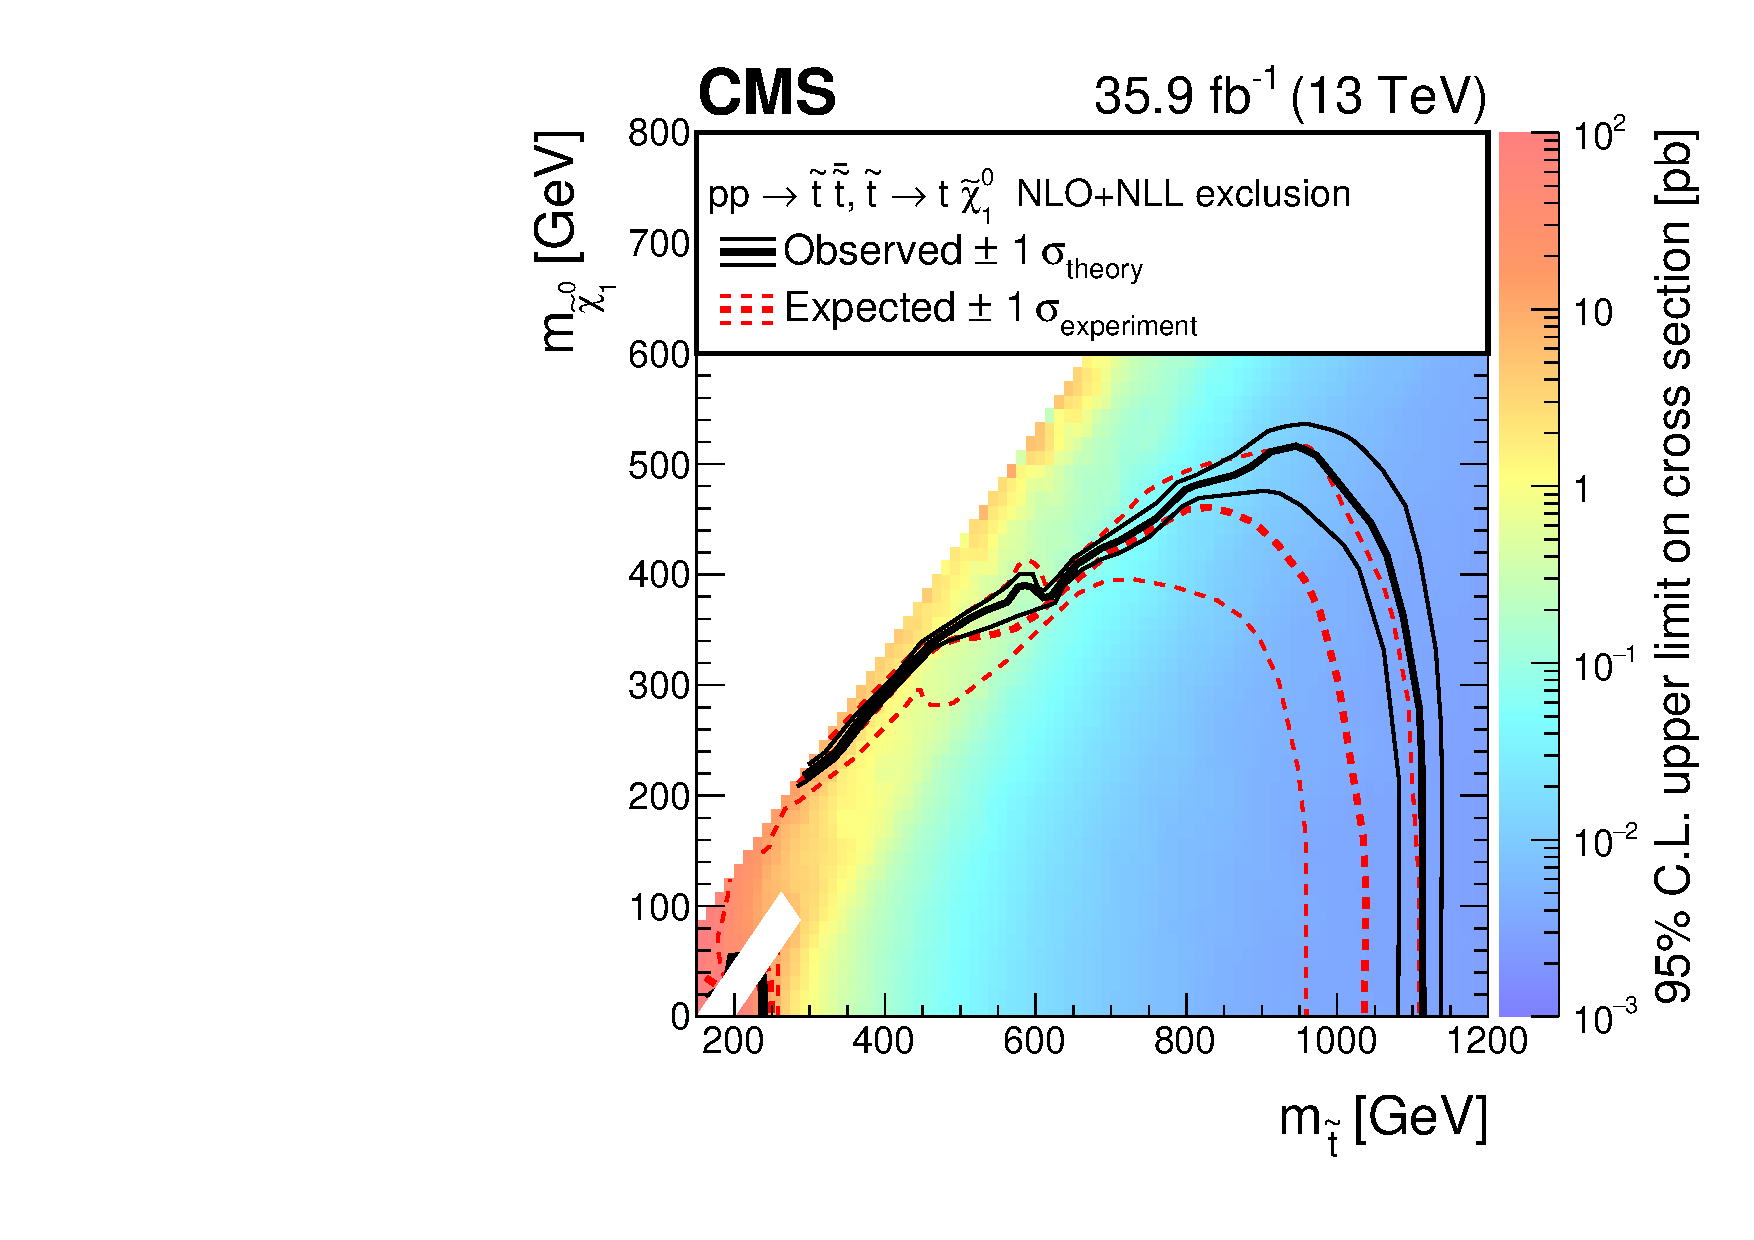
\includegraphics[width=0.8\textwidth]{figures/limits_T2tt.pdf}
\caption{Exclusion limits at 95\% CL (black line) and cross section
  upper limits at 95\% CL (color scale) for production of stop squarks
  decaying to top quarks and LSPs.}
\label{fig:stop:limits:t2tt}
\end{figure}

% T2bW exclusion plot, taken from public results page. Published.
\begin{figure}[htbp]
\centering
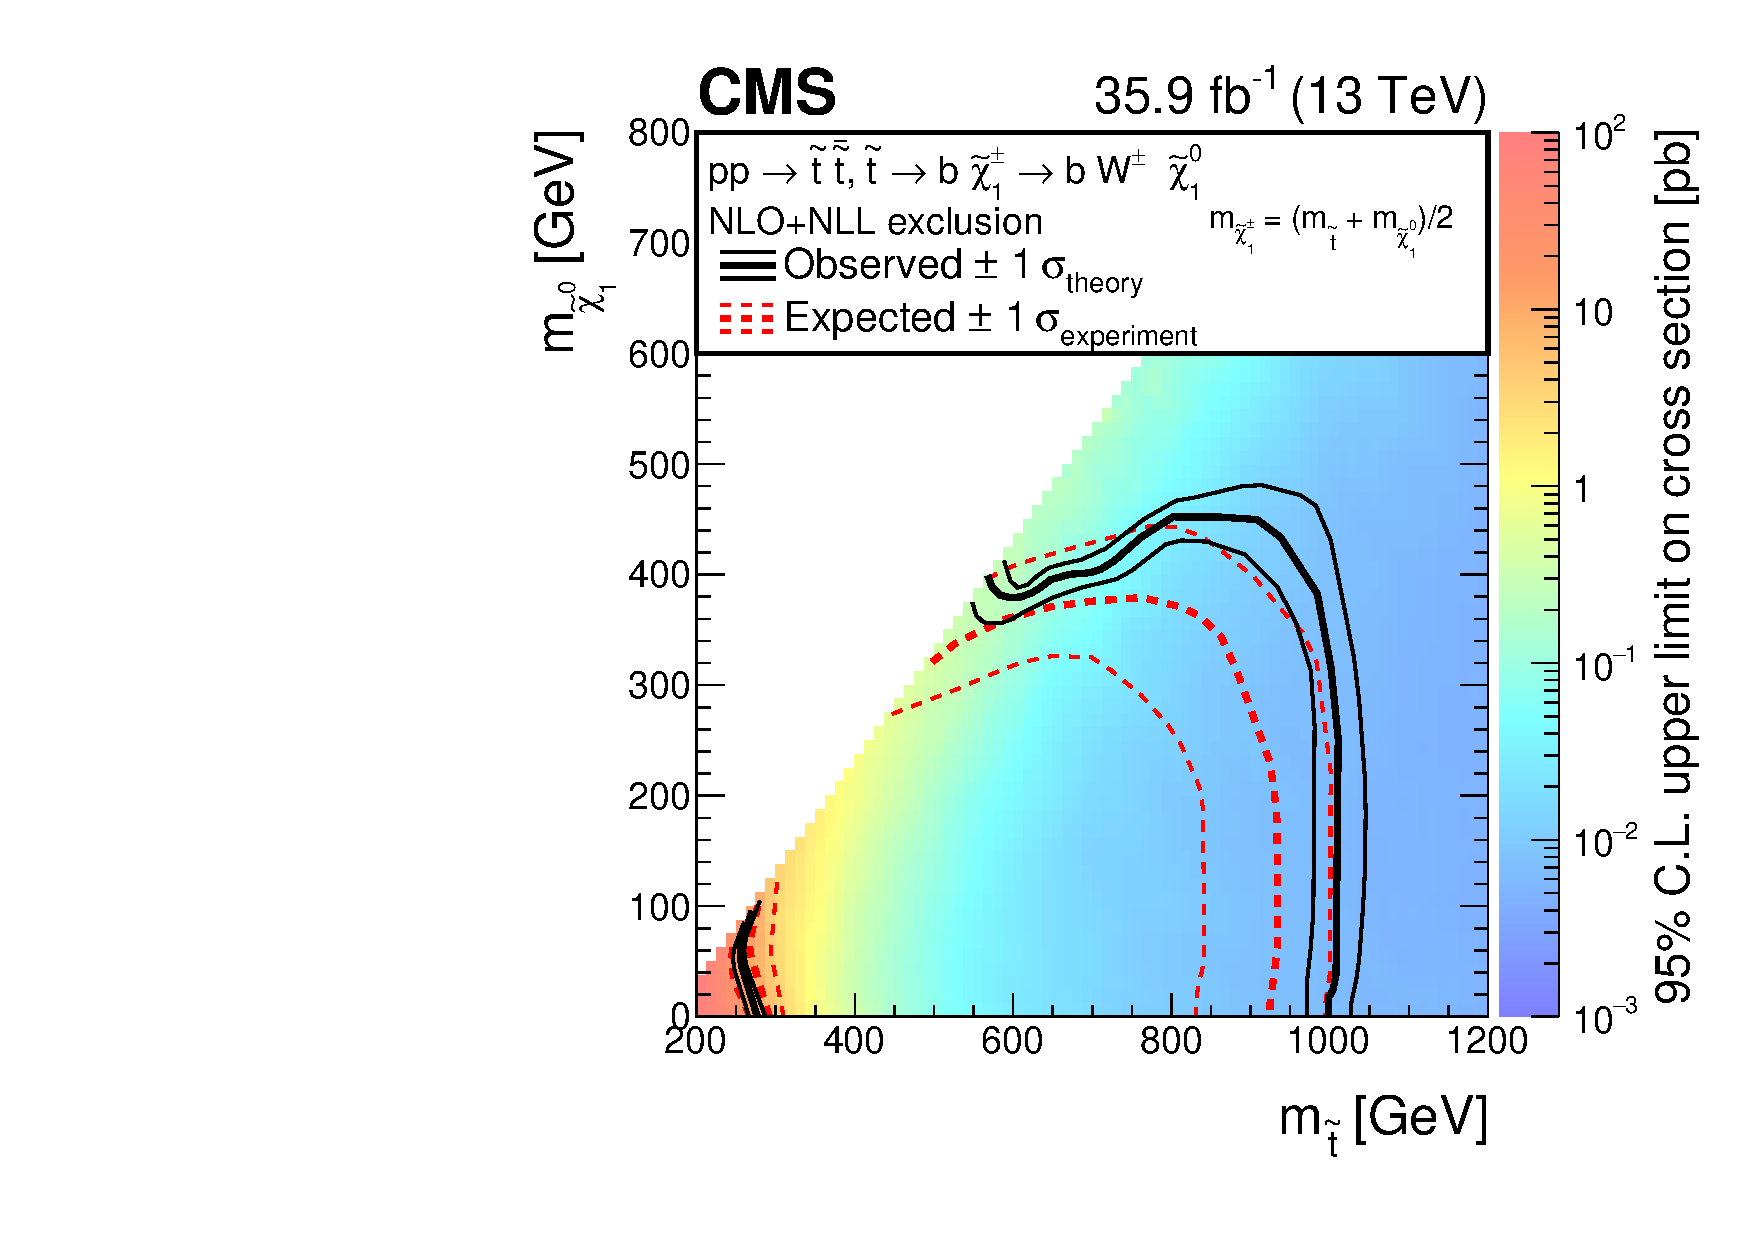
\includegraphics[width=0.8\textwidth]{figures/limits_T2bW.pdf}
\caption{Exclusion limits at 95\% CL (black line) and cross section
  upper limits at 95\% CL (color scale) for production of stop squarks
  decaying to bottom quarks and charginos, with charginos decaying to
  W-bosons and LSPs.}
\label{fig:stop:limits:t2bw}
\end{figure}

% T2tb exclusion plot, taken from public results page. Published.
\begin{figure}[htbp]
\centering
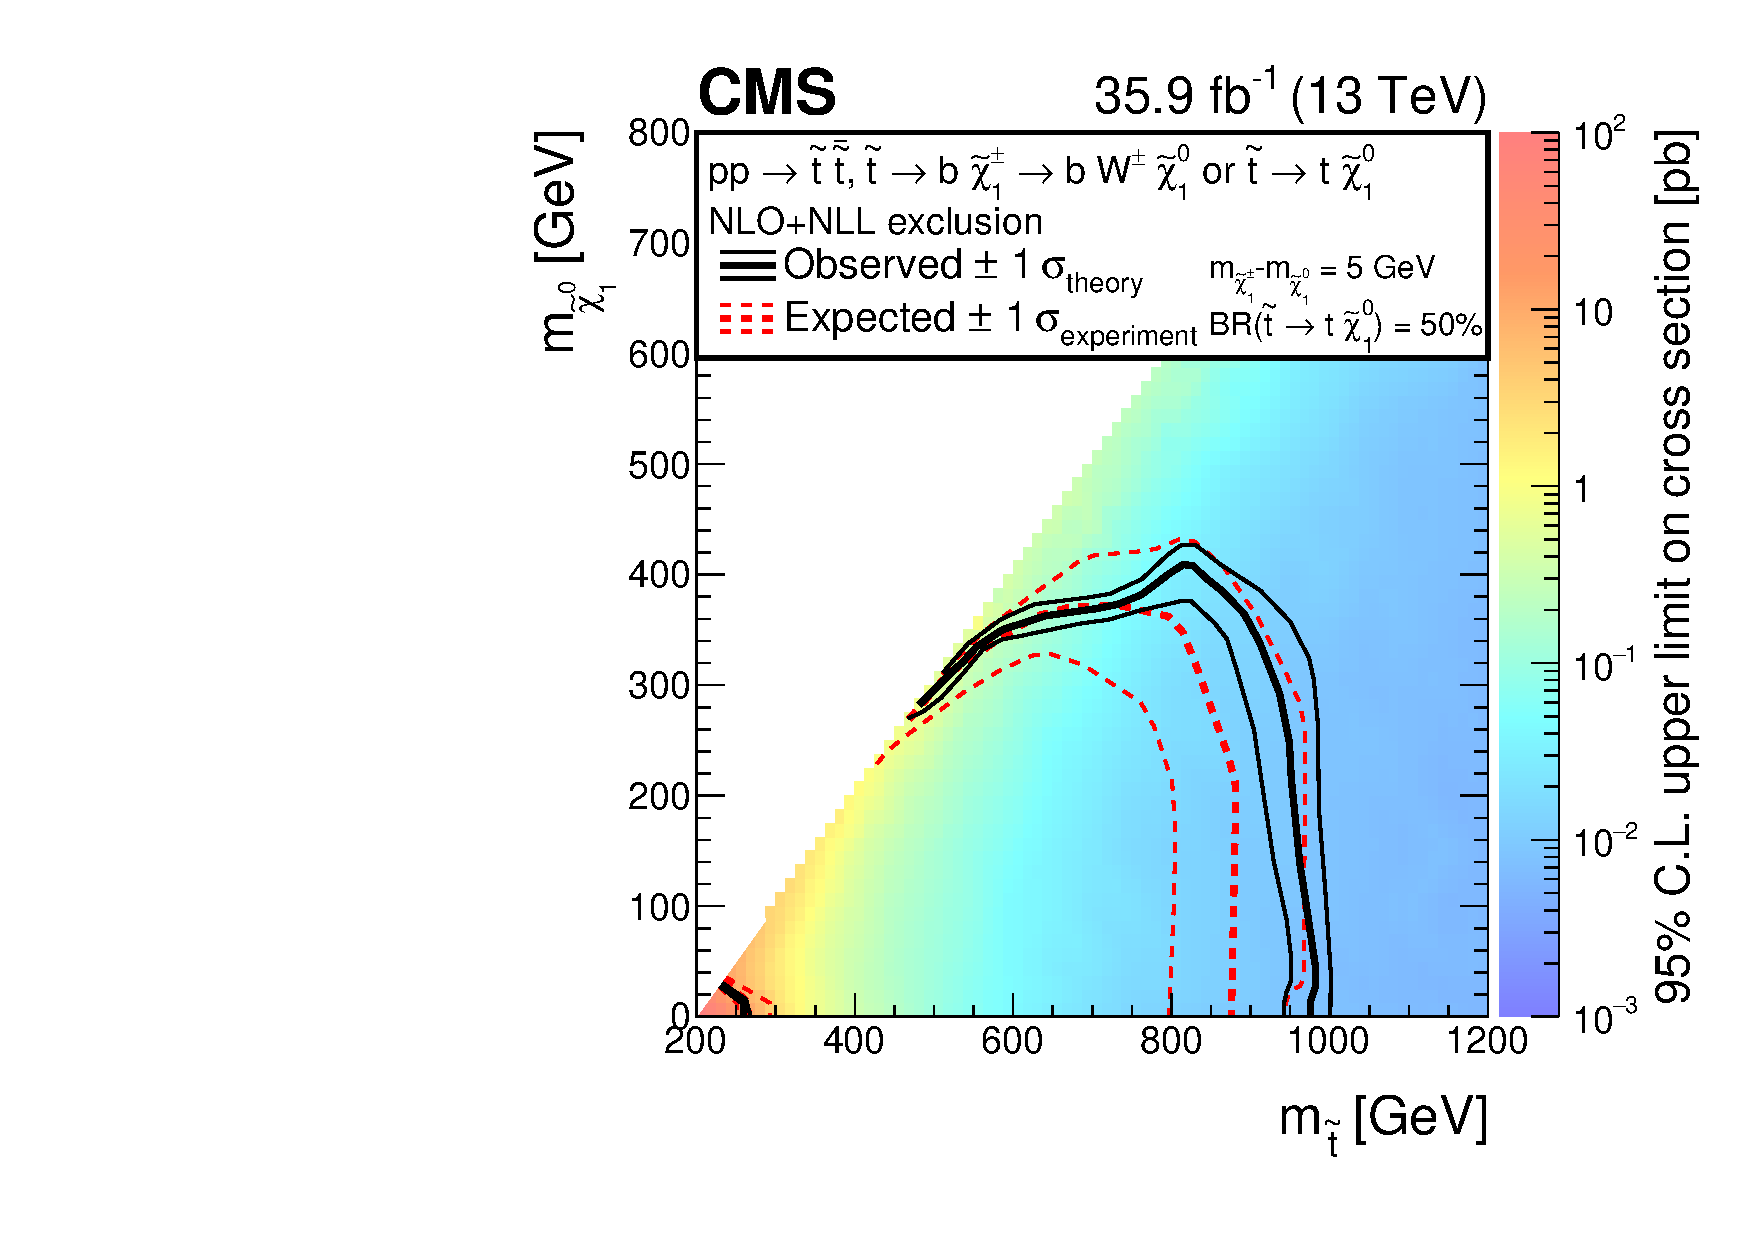
\includegraphics[width=0.8\textwidth]{figures/limits_T2tb.pdf}
\caption{Exclusion limits at 95\% CL (black line) and cross section
  upper limits at 95\% CL (color scale) for production of stop squarks
  decaying half to top quarks and LSPs and half to bottom quarks and
  charginos.}
\label{fig:stop:limits:t2tb}
\end{figure}


\section{Conclusion}
\label{sec:stop:conclusion}

We have performed a search for three models of stop squark pair production
and decay to single lepton final states using data from the CMS
experiment. The data, collected in 2016, correspond to 35.9
fb\textsuperscript{-1} of luminosity. We selected events containing a
single isolated electron or muon, multiple jets, and large
$\met$. The results were consistent with the presence of Standard
Model physics only. We set exclusion
limits on these models; at the 95\% confidence level, these exclusions
include stop squarks up to about 1000 GeV for massless neutralinos,
and neutralino masses up to 515 GeV for a stop mass of 950 GeV.

\section{Acknowledgements}
\label{sec:stop:acknowledgements}

Although the bulk of this analysis was the work of a few physicists,
the analysis would not be possible without the efforts of the entire
CMS collaboration, more than 3,000 members strong. They were responsible
for maintaining the detector, software, and computing platforms
necessary to perform the analysis. In addition, numerous members
contributed feedback that enhanced the quality of the analysis.

The 2016 analysis was published singly in JHEP \cite{stop1l}, and an
earlier version based on 2015 data was published, combined with an
all-hadronic stop search, in EPJ \cite{combination0l}.



\chapter{Just a Test}
This is only a test.
\section{A section}
Lorem ipsum dolor sit amet, consectetuer adipiscing elit. Nulla odio
sem, bibendum ut, aliquam ac, facilisis id, tellus. Nam posuere pede
sit amet ipsum. Etiam dolor. In sodales eros quis pede.  Quisque sed
nulla et ligula vulputate lacinia. In venenatis, ligula id semper
feugiat, ligula odio adipiscing libero, eget mollis nunc erat id orci.
Nullam ante dolor, rutrum eget, vestibulum euismod, pulvinar at, nibh.
In sapien. Quisque ut arcu. Suspendisse potenti. Cras consequat cursus
nulla.

\subsection{A Figure Example}
\label{ssec:figure_example}

This subsection shows a sample figure.

\begin{figure}[h] 
  \centering
  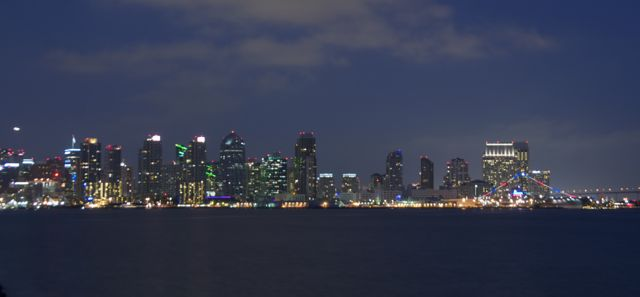
\includegraphics[width=0.5\textwidth]{sandiego}
  \caption[A picture of San Diego. Short figure caption must be \protect{$< 4$} lines in the list of figures]
{A picture of San Diego.  Short figure caption must be \protect{$< 4$} lines in the list of figures and match the start of the main figure caption verbatim. Note that figures must be on their own line (no neighboring text) and captions must be single-spaced and appear \protect\textit{below} the figure.  Captions can be as long as you want, but if they are longer than 4 lines in the list of figures, you must provide a short figure caption.\index{SanDiego}}
  \label{fig:sandiego}
\end{figure}

\subsection{A Table Example}

While in Section \ref{ssec:figure_example} Figure \ref{fig:sandiego} we had a majestic figure, here we provide a crazy table example.


%%%% TABLE 1 %%%%
\vspace{0.25in}
\begin{table}[!ht]
\caption[A table of when I get hungry.  Short table caption must be \protect{$< 4$} lines in the list of tables]{A table of when I get hungry. Short table caption must be \protect{$< 4$} lines in the list of tables and match the start of the main table caption verbatim.  Note that tables must be on their own line (no neighboring text) and captions must be single-spaced and appear \protect\textit{above} the table.  Captions can be as long as you want, but if they are longer than 4 lines in the list of figures, you must provide a short figure caption.}

\vspace{-0.25in}
\begin{center}
\begin{tabular}{|p{1in}|p{2in}|p{3in}|}

\hline
Time of day & Hunger Level & Preferred Food \\

\hline
8am & high & IHOP (French Toast) \\

\hline
noon & medium & Croutons (Tomato Basil Soup \& Granny Smith Chicken Salad) \\

\hline
5pm & high & Bombay Coast (Saag Paneer) or Hi Thai (Pad See Ew) \\

\hline
8pm & medium & Yogurt World (froyo!) \\

\hline
\end{tabular}
\end{center}
\label{tab:analysis3}
\end{table}



%% APPENDIX
\appendix
\chapter{Final notes}
What to do about things \cite{Martin_1983}.  What did he say \cite{Rilling_Insel_1999}.
  Remove me in case of abdominal pain.



%% END MATTER
% \printindex %% Uncomment to display the index
% \nocite{}  %% Put any references that you want to include in the bib 
%               but haven't cited in the braces.
\bibliographystyle{abbrv}  %% Try to mimic the style used in HEP
%\setlength{\bibleftmargin}{0.25in}  % indent each item
%\setlength{\bibindent}{-\bibleftmargin}  % unindent the first line
%\def\baselinestretch{1.0}  % force single spacing
%\setlength{\bibitemsep}{0.16in}  % add extra space between items
\bibliography{dissertation}  %% This looks for the bibliography in dissertation.bib
%                          which should be formatted as a bibtex file.
%                          and needs to be separately compiled into a bbl file.
\end{document}

